% Options for packages loaded elsewhere
\PassOptionsToPackage{unicode}{hyperref}
\PassOptionsToPackage{hyphens}{url}
\PassOptionsToPackage{dvipsnames,svgnames,x11names}{xcolor}
%
\documentclass[
  letterpaper,
  DIV=11,
  numbers=noendperiod]{scrreprt}

\usepackage{amsmath,amssymb}
\usepackage{lmodern}
\usepackage{iftex}
\ifPDFTeX
  \usepackage[T1]{fontenc}
  \usepackage[utf8]{inputenc}
  \usepackage{textcomp} % provide euro and other symbols
\else % if luatex or xetex
  \usepackage{unicode-math}
  \defaultfontfeatures{Scale=MatchLowercase}
  \defaultfontfeatures[\rmfamily]{Ligatures=TeX,Scale=1}
\fi
% Use upquote if available, for straight quotes in verbatim environments
\IfFileExists{upquote.sty}{\usepackage{upquote}}{}
\IfFileExists{microtype.sty}{% use microtype if available
  \usepackage[]{microtype}
  \UseMicrotypeSet[protrusion]{basicmath} % disable protrusion for tt fonts
}{}
\makeatletter
\@ifundefined{KOMAClassName}{% if non-KOMA class
  \IfFileExists{parskip.sty}{%
    \usepackage{parskip}
  }{% else
    \setlength{\parindent}{0pt}
    \setlength{\parskip}{6pt plus 2pt minus 1pt}}
}{% if KOMA class
  \KOMAoptions{parskip=half}}
\makeatother
\usepackage{xcolor}
\setlength{\emergencystretch}{3em} % prevent overfull lines
\setcounter{secnumdepth}{5}
% Make \paragraph and \subparagraph free-standing
\ifx\paragraph\undefined\else
  \let\oldparagraph\paragraph
  \renewcommand{\paragraph}[1]{\oldparagraph{#1}\mbox{}}
\fi
\ifx\subparagraph\undefined\else
  \let\oldsubparagraph\subparagraph
  \renewcommand{\subparagraph}[1]{\oldsubparagraph{#1}\mbox{}}
\fi

\usepackage{color}
\usepackage{fancyvrb}
\newcommand{\VerbBar}{|}
\newcommand{\VERB}{\Verb[commandchars=\\\{\}]}
\DefineVerbatimEnvironment{Highlighting}{Verbatim}{commandchars=\\\{\}}
% Add ',fontsize=\small' for more characters per line
\usepackage{framed}
\definecolor{shadecolor}{RGB}{241,243,245}
\newenvironment{Shaded}{\begin{snugshade}}{\end{snugshade}}
\newcommand{\AlertTok}[1]{\textcolor[rgb]{0.68,0.00,0.00}{#1}}
\newcommand{\AnnotationTok}[1]{\textcolor[rgb]{0.37,0.37,0.37}{#1}}
\newcommand{\AttributeTok}[1]{\textcolor[rgb]{0.40,0.45,0.13}{#1}}
\newcommand{\BaseNTok}[1]{\textcolor[rgb]{0.68,0.00,0.00}{#1}}
\newcommand{\BuiltInTok}[1]{\textcolor[rgb]{0.00,0.23,0.31}{#1}}
\newcommand{\CharTok}[1]{\textcolor[rgb]{0.13,0.47,0.30}{#1}}
\newcommand{\CommentTok}[1]{\textcolor[rgb]{0.37,0.37,0.37}{#1}}
\newcommand{\CommentVarTok}[1]{\textcolor[rgb]{0.37,0.37,0.37}{\textit{#1}}}
\newcommand{\ConstantTok}[1]{\textcolor[rgb]{0.56,0.35,0.01}{#1}}
\newcommand{\ControlFlowTok}[1]{\textcolor[rgb]{0.00,0.23,0.31}{#1}}
\newcommand{\DataTypeTok}[1]{\textcolor[rgb]{0.68,0.00,0.00}{#1}}
\newcommand{\DecValTok}[1]{\textcolor[rgb]{0.68,0.00,0.00}{#1}}
\newcommand{\DocumentationTok}[1]{\textcolor[rgb]{0.37,0.37,0.37}{\textit{#1}}}
\newcommand{\ErrorTok}[1]{\textcolor[rgb]{0.68,0.00,0.00}{#1}}
\newcommand{\ExtensionTok}[1]{\textcolor[rgb]{0.00,0.23,0.31}{#1}}
\newcommand{\FloatTok}[1]{\textcolor[rgb]{0.68,0.00,0.00}{#1}}
\newcommand{\FunctionTok}[1]{\textcolor[rgb]{0.28,0.35,0.67}{#1}}
\newcommand{\ImportTok}[1]{\textcolor[rgb]{0.00,0.46,0.62}{#1}}
\newcommand{\InformationTok}[1]{\textcolor[rgb]{0.37,0.37,0.37}{#1}}
\newcommand{\KeywordTok}[1]{\textcolor[rgb]{0.00,0.23,0.31}{#1}}
\newcommand{\NormalTok}[1]{\textcolor[rgb]{0.00,0.23,0.31}{#1}}
\newcommand{\OperatorTok}[1]{\textcolor[rgb]{0.37,0.37,0.37}{#1}}
\newcommand{\OtherTok}[1]{\textcolor[rgb]{0.00,0.23,0.31}{#1}}
\newcommand{\PreprocessorTok}[1]{\textcolor[rgb]{0.68,0.00,0.00}{#1}}
\newcommand{\RegionMarkerTok}[1]{\textcolor[rgb]{0.00,0.23,0.31}{#1}}
\newcommand{\SpecialCharTok}[1]{\textcolor[rgb]{0.37,0.37,0.37}{#1}}
\newcommand{\SpecialStringTok}[1]{\textcolor[rgb]{0.13,0.47,0.30}{#1}}
\newcommand{\StringTok}[1]{\textcolor[rgb]{0.13,0.47,0.30}{#1}}
\newcommand{\VariableTok}[1]{\textcolor[rgb]{0.07,0.07,0.07}{#1}}
\newcommand{\VerbatimStringTok}[1]{\textcolor[rgb]{0.13,0.47,0.30}{#1}}
\newcommand{\WarningTok}[1]{\textcolor[rgb]{0.37,0.37,0.37}{\textit{#1}}}

\providecommand{\tightlist}{%
  \setlength{\itemsep}{0pt}\setlength{\parskip}{0pt}}\usepackage{longtable,booktabs,array}
\usepackage{calc} % for calculating minipage widths
% Correct order of tables after \paragraph or \subparagraph
\usepackage{etoolbox}
\makeatletter
\patchcmd\longtable{\par}{\if@noskipsec\mbox{}\fi\par}{}{}
\makeatother
% Allow footnotes in longtable head/foot
\IfFileExists{footnotehyper.sty}{\usepackage{footnotehyper}}{\usepackage{footnote}}
\makesavenoteenv{longtable}
\usepackage{graphicx}
\makeatletter
\def\maxwidth{\ifdim\Gin@nat@width>\linewidth\linewidth\else\Gin@nat@width\fi}
\def\maxheight{\ifdim\Gin@nat@height>\textheight\textheight\else\Gin@nat@height\fi}
\makeatother
% Scale images if necessary, so that they will not overflow the page
% margins by default, and it is still possible to overwrite the defaults
% using explicit options in \includegraphics[width, height, ...]{}
\setkeys{Gin}{width=\maxwidth,height=\maxheight,keepaspectratio}
% Set default figure placement to htbp
\makeatletter
\def\fps@figure{htbp}
\makeatother
\newlength{\cslhangindent}
\setlength{\cslhangindent}{1.5em}
\newlength{\csllabelwidth}
\setlength{\csllabelwidth}{3em}
\newlength{\cslentryspacingunit} % times entry-spacing
\setlength{\cslentryspacingunit}{\parskip}
\newenvironment{CSLReferences}[2] % #1 hanging-ident, #2 entry spacing
 {% don't indent paragraphs
  \setlength{\parindent}{0pt}
  % turn on hanging indent if param 1 is 1
  \ifodd #1
  \let\oldpar\par
  \def\par{\hangindent=\cslhangindent\oldpar}
  \fi
  % set entry spacing
  \setlength{\parskip}{#2\cslentryspacingunit}
 }%
 {}
\usepackage{calc}
\newcommand{\CSLBlock}[1]{#1\hfill\break}
\newcommand{\CSLLeftMargin}[1]{\parbox[t]{\csllabelwidth}{#1}}
\newcommand{\CSLRightInline}[1]{\parbox[t]{\linewidth - \csllabelwidth}{#1}\break}
\newcommand{\CSLIndent}[1]{\hspace{\cslhangindent}#1}

\KOMAoption{captions}{tableheading}
\makeatletter
\makeatother
\makeatletter
\@ifpackageloaded{bookmark}{}{\usepackage{bookmark}}
\makeatother
\makeatletter
\@ifpackageloaded{caption}{}{\usepackage{caption}}
\AtBeginDocument{%
\ifdefined\contentsname
  \renewcommand*\contentsname{Table of contents}
\else
  \newcommand\contentsname{Table of contents}
\fi
\ifdefined\listfigurename
  \renewcommand*\listfigurename{List of Figures}
\else
  \newcommand\listfigurename{List of Figures}
\fi
\ifdefined\listtablename
  \renewcommand*\listtablename{List of Tables}
\else
  \newcommand\listtablename{List of Tables}
\fi
\ifdefined\figurename
  \renewcommand*\figurename{Figure}
\else
  \newcommand\figurename{Figure}
\fi
\ifdefined\tablename
  \renewcommand*\tablename{Table}
\else
  \newcommand\tablename{Table}
\fi
}
\@ifpackageloaded{float}{}{\usepackage{float}}
\floatstyle{ruled}
\@ifundefined{c@chapter}{\newfloat{codelisting}{h}{lop}}{\newfloat{codelisting}{h}{lop}[chapter]}
\floatname{codelisting}{Listing}
\newcommand*\listoflistings{\listof{codelisting}{List of Listings}}
\makeatother
\makeatletter
\@ifpackageloaded{caption}{}{\usepackage{caption}}
\@ifpackageloaded{subcaption}{}{\usepackage{subcaption}}
\makeatother
\makeatletter
\@ifpackageloaded{tcolorbox}{}{\usepackage[many]{tcolorbox}}
\makeatother
\makeatletter
\@ifundefined{shadecolor}{\definecolor{shadecolor}{rgb}{.97, .97, .97}}
\makeatother
\makeatletter
\makeatother
\ifLuaTeX
  \usepackage{selnolig}  % disable illegal ligatures
\fi
\IfFileExists{bookmark.sty}{\usepackage{bookmark}}{\usepackage{hyperref}}
\IfFileExists{xurl.sty}{\usepackage{xurl}}{} % add URL line breaks if available
\urlstyle{same} % disable monospaced font for URLs
\hypersetup{
  pdftitle={Deep Reinforcement Learning},
  pdfauthor={Julien Vitay},
  colorlinks=true,
  linkcolor={blue},
  filecolor={Maroon},
  citecolor={Blue},
  urlcolor={Blue},
  pdfcreator={LaTeX via pandoc}}

\title{Deep Reinforcement Learning}
\author{Julien Vitay}
\date{}

\begin{document}
\maketitle
\ifdefined\Shaded\renewenvironment{Shaded}{\begin{tcolorbox}[sharp corners, boxrule=0pt, frame hidden, borderline west={3pt}{0pt}{shadecolor}, enhanced, interior hidden, breakable]}{\end{tcolorbox}}\fi

\renewcommand*\contentsname{Table of contents}
{
\hypersetup{linkcolor=}
\setcounter{tocdepth}{2}
\tableofcontents
}
\bookmarksetup{startatroot}

\hypertarget{overview}{%
\chapter*{Overview}\label{overview}}
\addcontentsline{toc}{chapter}{Overview}

\markboth{Overview}{Overview}

The goal of this document is to keep track the state-of-the-art in deep
reinforcement learning. It starts with basics in reinforcement learning
and deep learning to introduce the notations and covers different
classes of deep RL methods, value-based or policy-based, model-free or
model-based, etc.

Different classes of deep RL methods can be identified. This document
will focus on the following ones:

\begin{enumerate}
\def\labelenumi{\arabic{enumi}.}
\tightlist
\item
  Value-based algorithms (DQN\ldots) used mostly for discrete problems
  like video games.
\item
  Policy-gradient algorithms (A3C, DDPG\ldots) used for continuous
  control problems such as robotics.
\item
  Recurrent attention models (RAM\ldots) for partially observable
  problems.
\item
  Model-based RL to reduce the sample complexity by incorporating a
  model of the environment.
\item
  Application of deep RL to robotics
\end{enumerate}

One could extend the list and talk about hierarchical RL, inverse RL,
imitation-based RL, etc\ldots{}

\textbf{Additional resources}

See Li (2017), Arulkumaran et al. (2017) and Mousavi et al. (2018) for
recent overviews of deep RL.

The CS294 course of Sergey Levine at Berkeley is incredibly complete:
\url{http://rll.berkeley.edu/deeprlcourse/}. The Reinforcement Learning
course by David Silver at UCL covers also the whole field:
\url{http://www0.cs.ucl.ac.uk/staff/d.silver/web/Teaching.html}.

This series of posts from Arthur Juliani
\url{https://medium.com/emergent-future/simple-reinforcement-learning-with-tensorflow-part-0-q-learning-with-tables-and-neural-networks-d195264329d0}
also provide a very good introduction to deep RL, associated to code
samples using tensorflow.

\textbf{Notes}

This document is meant to stay \emph{work in progress} forever, as new
algorithms will be added as they are published. Feel free to comment,
correct, suggest, pull request by writing to
\href{mailto:julien.vitay@informatik.tu-chemnitz.de}{\nolinkurl{julien.vitay@informatik.tu-chemnitz.de}}.

For some reason, this document is better printed using chrome. Use the
single file version \href{./DeepRL.html}{here} and print it to pdf.
Alternatively, a pdf version generated using LaTeX is available
\href{./DeepRL.pdf}{here} (some images may disappear, as LaTeX does not
support .gif or .svg images).

The style is adapted from the Github-Markdown CSS template
\url{https://www.npmjs.com/package/github-markdown-css}. The document is
written in Pandoc's Markdown and converted to html and pdf using
pandoc-citeproc and pandoc-crossref.

Some figures are taken from the original publication (``Taken from'' or
``Source'' in the caption). Their copyright stays to the respective
authors, naturally. The rest is my own work and can be distributed,
reproduced and modified under CC-BY-SA-NC 4.0.

\textbf{Thanks}

Thanks to all the students who helped me dive into that exciting
research field, in particular: Winfried Lötzsch, Johannes Jung, Frank
Witscher, Danny Hofmann, Oliver Lange, Vinayakumar Murganoor.

\textbf{Copyright}

Except where otherwise noted, this work is licensed under a
\href{http://creativecommons.org/licenses/by-nc-sa/4.0}{Creative Commons
Attribution-NonCommercial-ShareAlike 4.0 International License}.

\bookmarksetup{startatroot}

\hypertarget{basics}{%
\chapter{Basics}\label{basics}}

Deep reinforcement learning (deep RL) is the integration of deep
learning methods, classically used in supervised or unsupervised
learning contexts, with reinforcement learning (RL), a well-studied
adaptive control method used in problems with delayed and partial
feedback (Sutton and Barto, 1998). This section starts with the basics
of RL, mostly to set the notations, and provides a quick overview of
deep neural networks.

\hypertarget{reinforcement-learning-and-markov-decision-process}{%
\section{Reinforcement learning and Markov Decision
Process}\label{reinforcement-learning-and-markov-decision-process}}

RL methods apply to problems where an agent interacts with an
environment in discrete time steps (Figure~\ref{fig-agentenv}). At time
\(t\), the agent is in state \(s_t\) and decides to perform an action
\(a_t\). At the next time step, it arrives in the state \(s_{t+1}\) and
obtains the reward \(r_{t+1}\). The goal of the agent is to maximize the
reward obtained on the long term. The textbook by Sutton and Barto
(1998) (updated in Sutton and Barto (2017)) defines the field
extensively.

\begin{figure}

{\centering 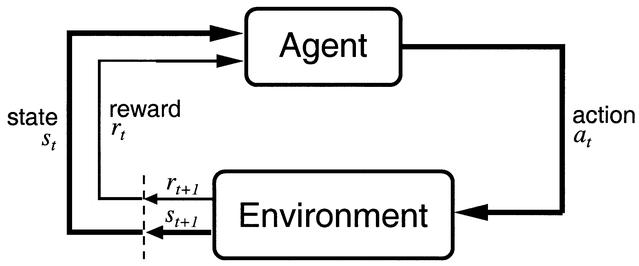
\includegraphics[width=0.5\textwidth,height=\textheight]{./img/rl-agent.jpg}

}

\caption{\label{fig-agentenv}Interaction between an agent and its
environment. Taken from Sutton and Barto (1998).}

\end{figure}

Reinforcement learning problems are described as \textbf{Markov Decision
Processes} (MDP) defined by five quantities:

\begin{itemize}
\tightlist
\item
  a state space \(\mathcal{S}\) where each state \(s\) respects the
  Markov property. It can be finite or infinite.
\item
  an action space \(\mathcal{A}\) of actions \(a\), which can be finite
  or infinite, discrete or continuous.
\item
  an initial state distribution \(p_0(s_0)\) (from which states is the
  agent likely to start).
\item
  a transition dynamics model with density \(p(s'|s, a)\), sometimes
  noted \(\mathcal{P}_{ss'}^a\). It defines the probability of arriving
  in the state \(s'\) at time \(t+1\) when being in the state \(s\) and
  performing the action \(a\).
\item
  a reward function
  \(r(s, a, s') : \mathcal{S}\times\mathcal{A}\times\mathcal{S} \rightarrow \Re\)
  defining the (stochastic) reward obtained after performing \(a\) in
  state \(s\) and arriving in \(s'\).
\end{itemize}

The behavior of the agent over time is a \textbf{trajectory} (also
called episode, history or roll-out)
\(\tau = (s_0, a_0, s_1, a_, \ldots, s_T, a_T)\) defined by the dynamics
of the MDP. Each transition occurs with a probability \(p(s'|s, a)\) and
provides a certain amount of reward defined by \(r(s, a, s')\). In
episodic tasks, the horizon \(T\) is finite, while in continuing tasks
\(T\) is infinite.

Importantly, the \textbf{Markov property} states that:

\[
    p(s_{t+1}|s_t, a_t) = p(s_{t+1}|s_t, a_t, s_{t-1}, a_{t-1}, \dots s_0, a_0)
\]

i.e.~you do not need the full history of the agent to predict where it
will arrive after an action. In simple problems, this is just a question
of providing enough information to the description of a state: if a
transition depends on what happened in the past, just put that
information in the state description.

If the Markov property is not met, RL methods may not converge (or
poorly). In many problems, one does not have access to the true states
of the agent, but one can only indirectly observe them. For example, in
a video game, the true state is defined by a couple of variables:
coordinates \((x, y)\) of the two players, position of the ball, speed,
etc. However, all you have access to are the raw pixels: sometimes the
ball may be hidden behind a wall or a tree, but it still exists in the
state space. Speed information is also not observable in a single frame.

In a \textbf{Partially Observable Markov Decision Process} (POMDP),
observations \(o_t\) come from a space \(\mathcal{O}\) and are linked to
underlying states using the density function \(p(o_t| s_t)\).
Observations are usually not Markov, so the full history of observations
\(h_t = (o_0, a_0, \dots o_t, a_t)\) is needed to solve the problem.

\hypertarget{policy-and-value-functions}{%
\subsection{Policy and value
functions}\label{policy-and-value-functions}}

The policy defines the behavior of the agent: which action should be
taken in each state. One distinguishes two kinds of policies:

\begin{itemize}
\tightlist
\item
  a stochastic policy \(\pi : \mathcal{S} \rightarrow P(\mathcal{A})\)
  defines the probability distribution \(P(\mathcal{A})\) of performing
  an action.
\item
  a deterministic policy \(\mu(s_t)\) is a discrete mapping of
  \(\mathcal{S} \rightarrow \mathcal{A}\).
\end{itemize}

The policy can be used to explore the environment and generate
trajectories of states, rewards and actions. The performance of a policy
is determined by estimating the \textbf{discounted return}, i.e.~the sum
of all rewards received from time step \(t\) onwards:

\[
    R_t = \sum_{k=0}^{T} \gamma^k \, r_{t+k+1}
\]

where \(0 < \gamma \leq 1\) is the discount rate and \(r_{t+1}\)
represents the reward obtained during the transition from \(s_t\) to
\(s_{t+1}\).

The \textbf{discount rate} \(\gamma\) is a critical hyperparameter of
RL: chosen too small, only immediate rewards will matter
(i.e.~participate to \(R_t\)) and the agent will be greedy. Chosen too
close from 1, hypothetical rewards delivered in one year from now will
count as much as slightly smaller rewards delivered for certain now.

If the task is episodic (\(T\) is finite, the trajectories ends after a
finite number of transitions), \(\gamma\) can be set to 1, but if the
task is continuing (\(T=\infty\), trajectories have no end), \(\gamma\)
must be chosen smaller than 1.

The Q-value of a state-action pair \((s, a)\) is defined as the expected
discounted return received if the agent takes \(a\) from a state \(s\)
and follows the policy distribution \(\pi\) thereafter:

\[
    Q^{\pi}(s, a) = \mathbb{E}_{\pi}[R_t | s_t = s, a_t=a]
\]

More precisely, the Q-value of a state-action pair is the mathematical
expectation of the return over all trajectories starting in \((s, a)\)
defined by the policy \(\pi\).

Similarly, the value of a state \(s\) is the expected discounted return
received if the agent starts in \(s\) and thereafter follows its policy
\(\pi\).

\[
    V^{\pi}(s) = \mathbb{E}_{\pi}[R_t | s_t = s]
\]

Obviously, these quantities depend on the states/actions themselves
(some chessboard configurations are intrinsically better than others,
i.e.~you are more likely to win from that state), but also on the policy
(if you can kill your opponent in one move - meaning you are in an
intrinsically good state - but systematically take the wrong decision
and lose, this is actually a bad state).

\hypertarget{bellman-equations}{%
\subsection{Bellman equations}\label{bellman-equations}}

The V- and Q-values are obviously linked with each other. The value of
state depend on the value of the actions possible in that state,
modulated by the probability that an action will be taken (i.e.~the
policy):

\begin{equation}\protect\hypertarget{eq-v-value}{}{
    V^{\pi}(s) = \sum_{a \in \mathcal{A}} \pi(s, a) \, Q^\pi(s,a)
}\label{eq-v-value}\end{equation}

For a deterministic policy (\(\pi(s, a) = 1\) if \(a=a^*\) and \(0\)
otherwise), the value of a state is the same as the value of the action
that will be systematically taken.

Noting that:

\begin{equation}\protect\hypertarget{eq-return}{}{
    R_t = r_{t+1} + \gamma R_{t+1}
}\label{eq-return}\end{equation}

i.e.~that the return at time \(t\) is the sum of the immediate reward
received during the next transition \(r_{t+1}\) and of the return at the
next state (\(R_{t+1}\), discounted by \(\gamma\)), we can also write:

\begin{equation}\protect\hypertarget{eq-q-value}{}{
    Q^{\pi}(s, a) = \sum_{s' \in \mathcal{S}} p(s'|s, a) [r(s, a, s') + \gamma \, V^\pi(s')]
}\label{eq-q-value}\end{equation}

The value of an action depends on which state you arrive in (\(s'\)),
with which probability (\(p(s'|s, a)\)) this transition occurs, how much
reward you receive immediately (\(r(s, a, s')\)) and how much you will
receive later (summarized by \(V^\pi(s')\)).

Putting together Equation~\ref{eq-v-value} and
Equation~\ref{eq-q-value}, we obtain the \textbf{Bellman equations}:

\[
    V^{\pi}(s) = \sum_{a \in \mathcal{A}} \pi(s, a) \, \sum_{s' \in \mathcal{S}} p(s'|s, a) [r(s, a, s') + \gamma \, V^\pi(s')]
\]

\[
    Q^{\pi}(s, a) = \sum_{s' \in \mathcal{S}} p(s'|s, a) [r(s, a, s') + \gamma \, \sum_{a' \in \mathcal{A}} \pi(s', a') \, Q^\pi(s',a')]
\]

The Bellman equations mean that the value of a state (resp. state-action
pair) depends on the value of all other states (resp. state-action
pairs), the current policy \(\pi\) and the dynamics of the MDP
(\(p(s'|s, a)\) and \(r(s, a, s')\)).

\begin{figure}

{\centering 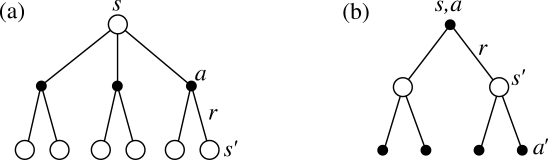
\includegraphics[width=0.5\textwidth,height=\textheight]{./img/backup.png}

}

\caption{\label{fig-backup}Backup diagrams corresponding to the Bellman
equations. Taken from Sutton and Barto (1998).}

\end{figure}

\hypertarget{dynamic-programming}{%
\subsection{Dynamic programming}\label{dynamic-programming}}

The interesting property of the Bellman equations is that, if the states
have the Markov property, they admit \emph{one and only one} solution.
This means that for a given policy, if the dynamics of the MDP are
known, it is possible to compute the value of all states or state-action
pairs by solving the Bellman equations for all states or state-action
pairs (\emph{policy evaluation}).

Once the values are known for a given policy, it is possible to improve
the policy by selecting with the highest probability the action with the
highest Q-value. For example, if the current policy chooses the action
\(a_1\) over \(a_2\) in \(s\) (\(\pi(s, a_1) > \pi(s, a_2)\)), but after
evaluating the policy it turns out that
\(Q^\pi(s, a_2) > Q^\pi(s, a_1)\) (the expected return after \(a_2\) is
higher than after \(a_1\)), it makes more sense to preferentially select
\(a_2\), as there is more reward afterwards. We can then create a new
policy \(\pi'\) where \(\pi'(s, a_2) > \pi'(s, a_1)\), which is is
\emph{better} policy than \(\pi\) as more reward can be gathered after
\(s\).

\begin{figure}

{\centering 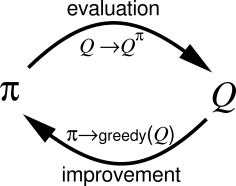
\includegraphics[width=0.2\textwidth,height=\textheight]{./img/dynamicprogramming.png}

}

\caption{\label{fig-dynamicprogramming}Dynamic programming alternates
between policy evaluation and policy improvement. Taken from Sutton and
Barto (1998).}

\end{figure}

\textbf{Dynamic programming} (DP) alternates between policy evaluation
and policy improvement. If the problem is Markov, it can be shown that
DP converges to the \emph{optimal policy} \(\pi^*\), i.e.~the policy
where the expected return is maximal in all states.

Note that by definition the optimal policy is \emph{deterministic} and
\emph{greedy}: if there is an action with a maximal Q-value for the
optimal policy, it should be systematically taken. For the optimal
policy \(\pi^*\), the Bellman equations become:

\[
    V^{*}(s) = \max_{a \in \mathcal{A}} \sum_{s \in \mathcal{S}} p(s' | s, a) \cdot [ r(s, a, s') + \gamma \cdot V^{*} (s') ]
\]

\[
    Q^{*}(s, a) = \sum_{s' \in \mathcal{S}} p(s' | s, a) \cdot [r(s, a, s') + \gamma \max_{a' \in \mathcal{A}} Q^* (s', a') ]
\]

Dynamic programming can only be used when:

\begin{itemize}
\tightlist
\item
  the dynamics of the MDP (\(p(s'|s, a)\) and \(r(s, a, s')\)) are fully
  known.
\item
  the number of states and state-action pairs is small (one Bellman
  equation per state or state/action to solve).
\end{itemize}

In practice, sample-based methods such as Monte-Carlo or temporal
difference are used.

\hypertarget{monte-carlo-sampling}{%
\subsection{Monte-Carlo sampling}\label{monte-carlo-sampling}}

\begin{figure}

{\centering 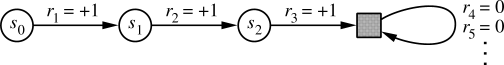
\includegraphics[width=0.5\textwidth,height=\textheight]{./img/unifiedreturn.png}

}

\caption{\label{fig-mc}Monte-Carlo methods accumulate rewards over a
complete episode. Taken from Sutton and Barto (1998).}

\end{figure}

When the environment is \emph{a priori} unknown, it has to be explored
in order to build estimates of the V or Q value functions. The key idea
of \textbf{Monte-Carlo} sampling (MC) is rather simple:

\begin{enumerate}
\def\labelenumi{\arabic{enumi}.}
\tightlist
\item
  Start from a state \(s_0\).
\item
  Perform an episode (sequence of state-action transitions) until a
  terminal state \(s_T\) is reached using your current policy \(\pi\).
\item
  Accumulate the rewards into the actual return for that episode
  \(R_t^{(e)} = \sum_{k=0}^T r_{t+k+1}\) for each time step.
\item
  Repeat often enough so that the value of a state \(s\) can be
  approximated by the average of many actual returns:
\end{enumerate}

\[V^\pi(s) = \mathbb{E}_\pi[R_t | s_t = s] \approx \frac{1}{M} \sum_{e=1}^M R_t^{(e)}\]

Monte-carlo sampling is a classical method to estimate quantities
defined by a mathematical expectation: the \emph{true} value of
\(V^\pi(s)\) is defined over \textbf{all} trajectories starting in
\(s\), what is impossible to compute in most problems. In MC methods,
the true value is approximated by the average of a sufficient number of
sampled trajectories, the million dollar question being: what means
\emph{sufficient}?

In practice, the estimated values are updated using continuous updates:

\[
    V^\pi(s) \leftarrow V^\pi(s) + \alpha (R_t - V^\pi(s))
\]

Q-values can also be approximated using the same procedure:

\[
    Q^\pi(s, a) \leftarrow Q^\pi(s, a) + \alpha (R_t - Q^\pi(s, a))
\]

The two main drawbacks of MC methods are:

\begin{enumerate}
\def\labelenumi{\arabic{enumi}.}
\tightlist
\item
  The task must be episodic, i.e.~stop after a finite amount of
  transitions. Updates are only applied at the end of an episode.
\item
  A sufficient level of exploration has to be ensured to make sure the
  estimates converge to the optimal values.
\end{enumerate}

The second issue is linked to the \textbf{exploration-exploitation}
dilemma: the episode is generated using the current policy (or a policy
derived from it, see later). If the policy always select the same
actions from the beginning (exploitation), the agent will never discover
better alternatives: the values will converge to a local minimum. If the
policy always pick randomly actions (exploration), the policy which is
evaluated is not the current policy \(\pi\), but the random policy. A
trade-off between the two therefore has to be maintained: usually a lot
of exploration at the beginning of learning to accumulate knowledge
about the environment, less towards the end to actually use the
knowledge and perform optimally.

There are two types of methods trying to cope with exploration:

\begin{itemize}
\tightlist
\item
  \textbf{On-policy} methods generate the episodes using the learned
  policy \(\pi\), but it has to be \emph{\(\epsilon\)-soft},
  i.e.~stochastic: it has to let a probability of at least \(\epsilon\)
  of selecting another action than the greedy action (the one with the
  highest estimated Q-value).
\item
  \textbf{Off-policy} methods use a second policy called the
  \emph{behavior policy} to generate the episodes, but learn a different
  policy for exploitation, which can even be deterministic.
\end{itemize}

\(\epsilon\)-soft policies are easy to create. The simplest one is the
\textbf{\(\epsilon\)-greedy} action selection method, which assigns a
probability \((1-\epsilon)\) of selecting the greedy action (the one
with the highest Q-value), and a probability \(\epsilon\) of selecting
any of the other available actions:

\[
    a_t = \begin{cases} a_t^* \quad \text{with probability} \quad (1 - \epsilon) \\
                       \text{any other action with probability } \epsilon \end{cases}
\]

Another solution is the \textbf{Softmax} (or Gibbs distribution) action
selection method, which assigns to each action a probability of being
selected depending on their relative Q-values:

\[
    P(s, a) = \frac{\exp Q^\pi(s, a) / \tau}{ \sum_b \exp Q^\pi(s, b) / \tau}
\]

\(\tau\) is a positive parameter called the temperature: high
temperatures cause the actions to be nearly equiprobable, while low
temperatures cause \(\tau\) is a positive parameter called the
temperature.

The advantage of off-policy methods is that domain knowledge can be used
to restrict the search in the state-action space. For example, only
moves actually played by chess experts in a given state will be actually
explored, not random stupid moves. The obvious drawback being that if
the optimal solution is not explored by the behavior policy, the agent
has no way to discover it by itself.

\hypertarget{temporal-difference}{%
\subsection{Temporal Difference}\label{temporal-difference}}

The main drawback of Monte-Carlo methods is that the task must be
composed of finite episodes. Not only is it not always possible, but
value updates have to wait for the end of the episode, what slows
learning down. \textbf{Temporal difference} methods simply replace the
actual return obtained after a state or an action, by an estimation
composed of the reward immediately received plus the value of the next
state or action, as in Equation~\ref{eq-return}:

\[
    R_t \approx r(s, a, s') + \gamma \, V^\pi(s') \approx r + \gamma \, Q^\pi(s', a')
\]

This gives us the following learning rules:

\[
    V^\pi(s) \leftarrow V^\pi(s) + \alpha (r(s, a, s') + \gamma \, V^\pi(s') - V^\pi(s))
\]

\[
    Q^\pi(s, a) \leftarrow Q^\pi(s, a) + \alpha (r(s, a, s') + \gamma \, Q^\pi(s', a') - Q^\pi(s, a))
\]

The quantity:

\[
 \delta = r(s, a, s') + \gamma \, V^\pi(s') - V^\pi(s)
\]

or:

\[
    \delta = r(s, a, s') + \gamma \, Q^\pi(s', a') - Q^\pi(s, a)
\]

is called the \textbf{reward-prediction error} (RPE) or \textbf{TD
error}: it defines the surprise between the current reward prediction
(\(V^\pi(s)\) or \(Q^\pi(s, a)\)) and the sum of the immediate reward
plus the reward prediction in the next state / after the next action.

\begin{itemize}
\tightlist
\item
  If \(\delta > 0\), the transition was positively surprising: one
  obtains more reward or lands in a better state than expected. The
  initial state or action was actually underrated, so its estimated
  value must be increased.
\item
  If \(\delta < 0\), the transition was negatively surprising. The
  initial state or action was overrated, its value must be decreased.
\item
  If \(\delta = 0\), the transition was fully predicted: one obtains as
  much reward as expected, so the values should stay as they are.
\end{itemize}

The main advantage of this learning method is that the update of the V-
or Q-value can be applied immediately after a transition: no need to
wait until the end of an episode, or even to have episodes at all: this
is called \textbf{online learning} and allows very fast learning from
single transitions. The main drawback is that the updates depend on
other estimates, which are initially wrong: it will take a while before
all estimates are correct.

\begin{figure}

{\centering 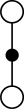
\includegraphics[width=0.03\textwidth,height=\textheight]{./img/backup-TD.png}

}

\caption{\label{fig-td}Temporal difference algorithms update values
after a single transition. Taken from Sutton and Barto (1998).}

\end{figure}

When learning Q-values directly, the question is which next action
\(a'\) should be used in the update rule: the action that will actually
be taken for the next transition (defined by \(\pi(s', a')\)), or the
greedy action (\(a^* = \text{argmax}_a Q^\pi(s', a)\)). This relates to
the \emph{on-policy / off-policy} distinction already seen for MC
methods:

\begin{itemize}
\tightlist
\item
  \textbf{On-policy} TD learning is called \textbf{SARSA}
  (state-action-reward-state-action). It uses the next action sampled
  from the policy \(\pi(s', a')\) to update the current transition. This
  selected action could be noted \(\pi(s')\) for simplicity. It is
  required that this next action will actually be performed for the next
  transition. The policy must be \(\epsilon\)-soft, for example
  \(\epsilon\)-greedy or softmax:
\end{itemize}

\[
    \delta = r(s, a, s') + \gamma \, Q^\pi(s', \pi(s')) - Q^\pi(s, a)
\]

\begin{itemize}
\tightlist
\item
  \textbf{Off-policy} TD learning is called \textbf{Q-learning}
  (Watkins, 1989). The greedy action in the next state (the one with the
  highest Q-value) is used to update the current transition. It does not
  mean that the greedy action will actually have to be selected for the
  next transition. The learned policy can therefore also be
  deterministic:
\end{itemize}

\[
    \delta = r(s, a, s') + \gamma \, \max_{a'} Q^\pi(s', a') - Q^\pi(s, a)
\]

In Q-learning, the behavior policy has to ensure exploration, while this
is achieved implicitly by the learned policy in SARSA, as it must be
\(\epsilon\)-soft. An easy way of building a behavior policy based on a
deterministic learned policy is \(\epsilon\)-greedy: the deterministic
action \(\mu(s_t)\) is chosen with probability 1 - \(\epsilon\), the
other actions with probability \(\epsilon\). In continuous action
spaces, additive noise (e.g.~Ohrstein-Uhlenbeck) can be added to the
action.

Alternatively, domain knowledge can be used to create the behavior
policy and restrict the search to meaningful actions: compilation of
expert moves in games, approximate solutions, etc. Again, the risk is
that the behavior policy never explores the actually optimal actions.
See \protect\hyperlink{off-policy-actor-critic}{off-policy actor-critic}
for more details on the difference between on-policy and off-policy
methods.

\hypertarget{eligibility-traces}{%
\subsection{Eligibility traces}\label{eligibility-traces}}

The main drawback of TD learning is that learning can be slow and
necessitate many transitions to converge (sample complexity). This is
particularly true when the problem provides \textbf{sparse rewards} (as
opposed to dense rewards). For example in a game like chess, a reward is
given only at the end of a game (+1 for winning, -1 for losing). All
other actions receive a reward of 0, although they are as important as
the last one in order to win.

Imagine you initialize all Q-values to 0 and apply Q-learning. During
the first episode, all actions but the last one will receive a reward
\(r(s, a, s')\) of 0 and arrive in a state where the greedy action has a
value \(Q^\pi(s', a')\) of 0, so the TD error \(\delta\) is 0 and their
Q-value will not change. Only the very last action will receive a
non-zero reward and update its value slightly (because of the learning
rate \(\alpha\)). When this episode is performed again, the last action
will again be updated, but also the one just before: \(Q^\pi(s', a')\)
is now different from 0 for this action, so the TD error is now
different from 0. It is straightforward to see that if the episode has a
length of 100 moves, the agent will need at least 100 episodes to
``backpropagate'' the final sparse reward to the first action of the
episode. In practice, this is even worse: the learning rate \(\alpha\)
and the discount rate \(\gamma\) will slow learning down even more. MC
methods suffer less from this problem, as the first action of the
episode would be updated using the actual return, which contains the
final reward (although it is discounted by \(\gamma\)).

\textbf{Eligibility traces} can be seen a trick to mix the advantages of
MC (faster updates) with the ones of TD (online learning, smaller
variance). The idea is that the TD error at time \(t\) (\(\delta_t\))
will be used not only to update the action taken at time \(t\)
(\(\Delta Q(s_t, a_t) = \alpha \, \delta_t\)), but also all the
preceding actions, which are also responsible for the success or failure
of the action taken at time \(t\). A parameter \(\lambda\) between 0 and
1 (decaying factor) controls how far back in time a single TD error
influences past actions. This is important when the policy is mostly
exploratory: initial actions may be mostly random and finally find the
the reward by chance. They should learn less from the reward than the
last one, otherwise they would be systematically reproduced.
Figure~\ref{fig-eligibilitytraces} shows the principle of eligibility
traces in a simple Gridworld environment.

\begin{figure}

{\centering 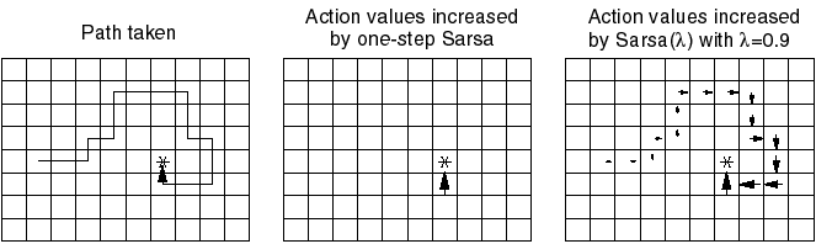
\includegraphics[width=0.8\textwidth,height=\textheight]{./img/gridworld-lambda.png}

}

\caption{\label{fig-eligibilitytraces}Principle of eligibility traces
applied to the Gridworld problem using SARSA(\(\lambda\)). Taken from
Sutton and Barto (1998).}

\end{figure}

There are many possible implementations of eligibility traces (Watkin's,
Peng, Tree Backup, etc. See the Chapter 12 of Sutton and Barto (2017)).
Generally, one distinguished a forward and a backward view of
eligibility traces.

\begin{itemize}
\tightlist
\item
  The \emph{forward view} considers that one transition \((s_t, a_t)\)
  gathers the TD errors made at future time steps \(t'\) and discounts
  them with the parameter \(\lambda\):
\end{itemize}

\[
    Q^\pi(s_t, a_t) \leftarrow  Q^\pi(s_t, a_t) + \alpha \, \sum_{t'=t}^T (\gamma \lambda)^{t'-t} \delta_{t'}
\]

From this equation, \(\gamma\) and \(\lambda\) seem to play a relatively
similar role, but remember that \(\gamma\) is also used in the TD error,
so they control different aspects of learning. The drawback of this
approach is that the future transitions at \(t'>t\) and their respective
TD errors must be known when updating the transition, so this prevents
online learning (the episode must be terminated to apply the updates).

\begin{itemize}
\tightlist
\item
  The \emph{backward view} considers that the TD error made at time
  \(t\) is sent backwards in time to all transitions previously
  executed. The easiest way to implement this is to update an
  eligibility trace \(e(s,a)\) for each possible transition, which is
  incremented every time a transition is visited and otherwise decays
  exponentially with a speed controlled by \(\lambda\):
\end{itemize}

\[
    e(s, a) = \begin{cases} e(s, a) + 1 \quad \text{if} \quad s=s_t \quad \text{and} \quad a=a_t \\
                            \lambda \, e(s, a) \quad \text{otherwise.}
              \end{cases}
\]

The Q-value of \textbf{all} transitions \((s, a)\) (not only the one
just executed) is then updated proportionally to the corresponding trace
and the current TD error:

\[
    Q^\pi(s, a) \leftarrow  Q^\pi(s, a) + \alpha \, e(s, a) \, \delta_{t} \quad \forall s, a
\]

The forward and backward implementations are equivalent: the first
requires to know the future, the second requires to update many
transitions at each time step. The best solution will depend on the
complexity of the problem.

TD learning, SARSA and Q-learning can all be efficiently extended using
eligibility traces. This gives the algorithms TD(\(\lambda\)),
SARSA(\(\lambda\)) and Q(\(\lambda\)), which can learn much faster than
their 1-step equivalent, at the cost of more computations.

\hypertarget{actor-critic-architectures}{%
\subsection{Actor-critic
architectures}\label{actor-critic-architectures}}

Let's consider the TD error based on state values:

\[
 \delta = r(s, a, s') + \gamma \, V^\pi(s') - V^\pi(s)
\]

As noted in the previous sections, the TD error represents how
surprisingly good (or bad) a transition between two states has been
(ergo the corresponding action). It can be used to update the value of
the state \(s_t\):

\[
    V^\pi(s) \leftarrow V^\pi(s) + \alpha \, \delta
\]

This allows to estimate the values of all states for the current policy.
However, this does not help to 1) directy select the best action or 2)
improve the policy. When only the V-values are given, one can only want
to reach the next state \(V^\pi(s')\) with the highest value: one needs
to know which action leads to this better state, i.e.~have a model of
the environment. Actually, one selects the action with the highest
Q-value:

\[
    Q^{\pi}(s, a) = \sum_{s' \in \mathcal{S}} p(s'|s, a) [r(s, a, s') + \gamma \, V^\pi(s')]
\]

An action may lead to a high-valued state, but with such a small
probability that it is actually not worth it. \(p(s'|s, a)\) and
\(r(s, a, s')\) therefore have to be known (or at least approximated),
what defeats the purpose of sample-based methods.

\begin{figure}

{\centering 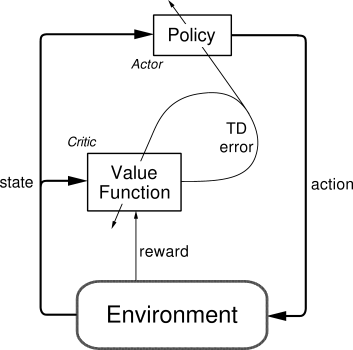
\includegraphics[width=0.3\textwidth,height=\textheight]{./img/actorcritic.png}

}

\caption{\label{fig-actorcritic}Actor-critic architecture (Sutton and
Barto, 1998).}

\end{figure}

\textbf{Actor-critic} architectures have been proposed to solve this
problem:

\begin{enumerate}
\def\labelenumi{\arabic{enumi}.}
\tightlist
\item
  The \textbf{critic} learns to estimate the value of a state
  \(V^\pi(s)\) and compute the RPE
  \(\delta = r(s, a, s') + \gamma \, V^\pi(s') - V^\pi(s)\).
\item
  The \textbf{actor} uses the RPE to update a \emph{preference} for the
  executed action: action with positive RPEs (positively surprising)
  should be reinforced (i.e.~taken again in the future), while actions
  with negative RPEs should be avoided in the future.
\end{enumerate}

The main interest of this architecture is that the actor can take any
form (neural network, decision tree), as long as it able to use the RPE
for learning. The simplest actor would be a softmax action selection
mechanism, which maintains a \emph{preference} \(p(s, a)\) for each
action and updates it using the TD error:

\[
    p(s, a) \leftarrow p(s, a) + \alpha \, \delta_t
\]

The policy uses the softmax rule on these preferences:

\[
    \pi(s, a) = \frac{p(s, a)}{\sum_a p(s, a)}
\]

Actor-critic algorithms learn at the same time two aspects of the
problem:

\begin{itemize}
\tightlist
\item
  A value function (e.g.~\(V^\pi(s)\)) to compute the TD error in the
  critic,
\item
  A policy \(\pi\) in the actor.
\end{itemize}

Classical TD learning only learn a value function (\(V^\pi(s)\) or
\(Q^\pi(s, a)\)): these methods are called \textbf{value-based} methods.
Actor-critic architectures are particularly important in \textbf{policy
search} methods.

\hypertarget{function-approximation}{%
\subsection{Function approximation}\label{function-approximation}}

All the methods presented before are \emph{tabular methods}, as one
needs to store one value per state-action pair: either the Q-value of
the action or a preference for that action. In most useful applications,
the number of values to store would quickly become prohibitive: when
working on raw images, the number of possible states alone is
untractable. Moreover, these algorithms require that each state-action
pair is visited a sufficient number of times to converge towards the
optimal policy: if a single state-action pair is never visited, there is
no guarantee that the optimal policy will be found. The problem becomes
even more obvious when considering \emph{continuous} state or action
spaces.

However, in a lot of applications, the optimal action to perform in two
very close states is likely to be the same: changing one pixel in a
video game does not change which action should be applied. It would
therefore be very useful to be able to \emph{interpolate} Q-values
between different states: only a subset of all state-action pairs has to
explored; the others will be ``guessed'' depending on the proximity
between the states and/or the actions. The problem is now
\textbf{generalization}, i.e.~transferring acquired knowledge to unseen
but similar situations.

This is where \textbf{function approximation} becomes useful: the
Q-values or the policy are not stored in a table, but rather learned by
a function approximator. The type of function approximator does not
really matter here: in deep RL we are of course interested in deep
neural networks, but any kind of regressor theoretically works (linear
algorithms, radial-basis function network, SVR\ldots).

\hypertarget{value-based-function-approximation}{%
\subsubsection*{Value-based function
approximation}\label{value-based-function-approximation}}
\addcontentsline{toc}{subsubsection}{Value-based function approximation}

In \textbf{value-based} methods, we want to approximate the Q-values
\(Q^\pi(s,a)\) of all possible state-action pairs for a given policy.
The function approximator depends on a set of parameters \(\theta\).
\(\theta\) can for example represent all the weights and biases of a
neural network. The approximated Q-value can now be noted
\(Q(s, a ;\theta)\) or \(Q_\theta(s, a)\). As the parameters will change
over time during learning, we can omit the time \(t\) from the notation.
Similarly, action selection is usually \(\epsilon\)-greedy or softmax,
so the policy \(\pi\) depends directly on the estimated Q-values and can
therefore on the parameters: it is noted \(\pi_\theta\).

\begin{figure}

{\centering 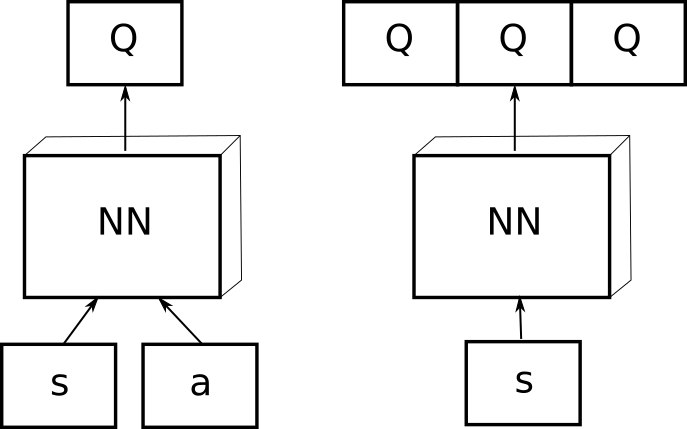
\includegraphics[width=0.5\textwidth,height=\textheight]{./img/functionapprox.png}

}

\caption{\label{fig-functionapprox}Function approximators can either
take a state-action pair as input and output the Q-value, or simply take
a state as input and output the Q-values of all possible actions.}

\end{figure}

There are basically two options regarding the structure of the function
approximator (Figure~\ref{fig-functionapprox}):

\begin{enumerate}
\def\labelenumi{\arabic{enumi}.}
\tightlist
\item
  The approximator takes a state-action pair \((s, a)\) as input and
  returns a single Q-value \(Q(s, a)\).
\item
  It takes a state \(s\) as input and returns the Q-value of all
  possible actions in that state.
\end{enumerate}

The second option is of course only possible when the action space is
discrete, but has the advantage to generalize better over similar
states.

The goal of a function approximator is to minimize a \emph{loss
function} (or cost function) \(\mathcal{L}(\theta)\), so that the
estimated Q-values converge for all state-pairs towards their target
value, depending on the chosen algorithm:

\begin{itemize}
\tightlist
\item
  Monte-Carlo methods: the Q-value of each \((s, a)\) pair should
  converge towards the expected return:
\end{itemize}

\[
    \mathcal{L}(\theta) = \mathbb{E}_\pi[(R_t - Q_\theta(s, a))^2]
\]

If we learn over \(N\) episodes of length \(T\), the loss function can
be approximated as:

\[
    \mathcal{L}(\theta) \approx \frac{1}{N} \sum_{e=1}^N \sum_{t = 1}^T [R^e_t - Q_\theta(s_t, a_t)]^2
\]

\begin{itemize}
\item
  Temporal difference methods: the Q-values should converge towards an
  estimation of the expected return.

  \begin{itemize}
  \tightlist
  \item
    For SARSA:
  \end{itemize}

  \[
    \mathcal{L}(\theta) = \mathbb{E}_\pi[(r(s, a, s') + \gamma \, Q_\theta(s', \pi(s')) - Q_\theta(s, a))^2]
    \]

  \begin{itemize}
  \tightlist
  \item
    For Q-learning:
  \end{itemize}

  \[
    \mathcal{L}(\theta) = \mathbb{E}_\pi[(r(s, a, s') + \gamma \, \max_{a'} Q_\theta(s', a') - Q_\theta(s, a))^2]
    \]
\end{itemize}

Any function approximator able to minimize these loss functions can be
used.

\hypertarget{policy-based-function-approximation}{%
\subsubsection*{Policy-based function
approximation}\label{policy-based-function-approximation}}
\addcontentsline{toc}{subsubsection}{Policy-based function
approximation}

In policy-based function approximation, we want to directly learn a
policy \(\pi_\theta(s, a)\) that maximizes the expected return of each
possible transition, i.e.~the ones which are selected by the policy. The
\textbf{objective function} to be maximized is defined over all
trajectories \(\tau = (s_0, a_0, s_1, a_1, \ldots, s_T, a_T)\)
conditioned by the policy:

\[
    J(\theta) = \mathbb{E}_{\tau \sim \rho_\theta} [R_t]
\]

In short, the learned policy \(\pi_\theta\) should only produce
trajectories \(\tau\) where each state is associated to a high return
\(R_t\) and avoid trajectories with low returns. Although this objective
function leads to the desired behavior, it is not computationally
tractable as we would need to integrate over all possible trajectories.
The methods presented in Section
\protect\hyperlink{policy-gradient-methods}{PolicyGradient} will provide
estimates of the gradient of this objective function.

\bookmarksetup{startatroot}

\hypertarget{deep-learning}{%
\chapter{Deep learning}\label{deep-learning}}

Deep RL uses deep neural networks as function approximators, allowing
complex representations of the value of state-action pairs to be
learned. This section provides a very quick overview of deep learning.
For additional details, refer to the excellent book of Goodfellow et al.
(2016).

\hypertarget{deep-neural-networks}{%
\subsection{Deep neural networks}\label{deep-neural-networks}}

A deep neural network (DNN) consists of one input layer \(\mathbf{x}\),
one or several hidden layers
\(\mathbf{h_1}, \mathbf{h_2}, \ldots, \mathbf{h_n}\) and one output
layer \(\mathbf{y}\) (Figure~\ref{fig-dnn}).

\begin{figure}

{\centering 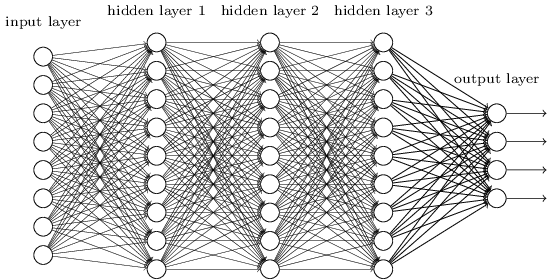
\includegraphics[width=0.6\textwidth,height=\textheight]{./img/dnn.png}

}

\caption{\label{fig-dnn}Architecture of a deep neural network. Figure
taken from Nielsen (2015), CC-BY-NC.}

\end{figure}

Each layer \(k\) (called \emph{fully-connected}) transforms the activity
of the previous layer (the vector \(\mathbf{h_{k-1}}\)) into another
vector \(\mathbf{h_{k}}\) by multiplying it with a \textbf{weight
matrix} \(W_k\), adding a \textbf{bias} vector \(\mathbf{b_k}\) and
applying a non-linear \textbf{activation function} \(f\).

\begin{equation}\protect\hypertarget{eq-fullyconnected}{}{
    \mathbf{h_{k}} = f(W_k \times \mathbf{h_{k-1}} + \mathbf{b_k})
}\label{eq-fullyconnected}\end{equation}

The activation function can theoretically be of any type as long as it
is non-linear (sigmoid, tanh\ldots), but modern neural networks use
preferentially the \textbf{Rectified Linear Unit} (ReLU) function
\(f(x) = \max(0, x)\) or its parameterized variants.

The goal of learning is to find the weights and biases \(\theta\)
minimizing a given \textbf{loss function} on a training set
\(\mathcal{D}\).

\begin{itemize}
\tightlist
\item
  In \emph{regression} problems, the \textbf{mean square error} (mse) is
  minimized:
\end{itemize}

\[
    \mathcal{L}(\theta) = \mathbb{E}_{\mathbf{x}, \mathbf{t} \in \mathcal{D}} [||\mathbf{t} - \mathbf{y}||^2]
\]

where \(\mathbf{x}\) is the input, \(\mathbf{t}\) the true output
(defined in the training set) and \(\mathbf{y}\) the prediction of the
NN for the input \(\mathbf{x}\). The closer the prediction from the true
value, the smaller the mse.

\begin{itemize}
\tightlist
\item
  In \emph{classification} problems, the \textbf{cross entropy} (or
  negative log-likelihood) is minimized:
\end{itemize}

\[
    \mathcal{L}(\theta) = - \mathbb{E}_{\mathbf{x}, \mathbf{t} \in \mathcal{D}} [\sum_i t_i \log y_i]
\]

where the log-likelihood of the prediction \(\mathbf{y}\) to match the
data \(\mathbf{t}\) is maximized over the training set. The mse could be
used for classification problems too, but the output layer usually has a
softmax activation function for classification problems, which works
nicely with the cross entropy loss function. See
\url{https://rdipietro.github.io/friendly-intro-to-cross-entropy-loss}
for the link between cross entropy and log-likelihood and
\url{https://deepnotes.io/softmax-crossentropy} for the interplay
between softmax and cross entropy.

Once the loss function is defined, it has to be minimized by searching
optimal values for the free parameters \(\theta\). This optimization
procedure is based on \textbf{gradient descent}, which is an iterative
procedure modifying estimates of the free parameters in the opposite
direction of the gradient of the loss function:

\[
\Delta \theta = -\eta \, \nabla_\theta \mathcal{L}(\theta) = -\eta \, \frac{\partial \mathcal{L}(\theta)}{\partial \theta}
\]

The learning rate \(\eta\) is chosen very small to ensure a smooth
convergence. Intuitively, the gradient (or partial derivative)
represents how the loss function changes when each parameter is slightly
increased. If the gradient w.r.t a single parameter (e.g.~a weight
\(w\)) is positive, increasing the weight increases the loss function
(i.e.~the error), so the weight should be slightly decreased instead. If
the gradient is negative, one should increase the weight.

The question is now to compute the gradient of the loss function w.r.t
all the parameters of the DNN, i.e.~each single weight and bias. The
solution is given by the \textbf{backpropagation} algorithm, which is
simply an application of the \textbf{chain rule} to feedforward neural
networks:

\[
    \frac{\partial \mathcal{L}(\theta)}{\partial W_k} = \frac{\partial \mathcal{L}(\theta)}{\partial \mathbf{y}} \times \frac{\partial \mathbf{y}}{\partial \mathbf{h_n}} \times \frac{\partial \mathbf{h_n}}{\partial \mathbf{h_{n-1}}} \times \ldots \times \frac{\partial \mathbf{h_k}}{\partial W_k}
\]

Each layer of the network adds a contribution to the gradient when going
\textbf{backwards} from the loss function to the parameters.
Importantly, all functions used in a NN are differentiable, i.e.~those
partial derivatives exist (and are easy to compute). For the fully
connected layer represented by Equation~\ref{eq-fullyconnected}, the
partial derivative is given by:

\[
    \frac{\partial \mathbf{h_{k}}}{\partial \mathbf{h_{k-1}}} = f'(W_k \times \mathbf{h_{k-1}} + \mathbf{b_k}) \, W_k
\]

and its dependency on the parameters is:

\[
    \frac{\partial \mathbf{h_{k}}}{\partial W_k} = f'(W_k \times \mathbf{h_{k-1}} + \mathbf{b_k}) \, \mathbf{h_{k-1}}
\] \[
    \frac{\partial \mathbf{h_{k}}}{\partial \mathbf{b_k}} = f'(W_k \times \mathbf{h_{k-1}} + \mathbf{b_k})
\]

Activation functions are chosen to have an easy-to-compute derivative,
such as the ReLU function:

\[
    f'(x) = \begin{cases} 1 \quad \text{if} \quad x > 0 \\ 0 \quad \text{otherwise.} \end{cases}
\]

Partial derivatives are automatically computed by the underlying
libraries, such as tensorflow, theano, pytorch, etc. The next step is
choose an \textbf{optimizer}, i.e.~a gradient-based optimization method
allow to modify the free parameters using the gradients. Optimizers do
not work on the whole training set, but use \textbf{minibatches} (a
random sample of training examples: their number is called the
\emph{batch size}) to compute iteratively the loss function. The most
popular optimizers are:

\begin{itemize}
\tightlist
\item
  SGD (stochastic gradient descent): vanilla gradient descent on random
  minibatches.
\item
  SGD with momentum (Nesterov or not): additional momentum to avoid
  local minima of the loss function.
\item
  Adagrad
\item
  Adadelta
\item
  RMSprop
\item
  Adam
\item
  Many others. Check the doc of keras to see what is available:
  \url{https://keras.io/optimizers}
\end{itemize}

See this useful post for a comparison of the different optimizers:
\url{http://ruder.io/optimizing-gradient-descent} (Ruder, 2016). The
common wisdom is that SGD with Nesterov momentum works best (i.e.~it
finds a better minimum) but its meta-parameters (learning rate,
momentum) are hard to find, while Adam works out-of-the-box, at the cost
of a slightly worse minimum. For deep RL, Adam is usually preferred, as
the goal is to quickly find a working solution, not to optimize it to
the last decimal.

Additional regularization mechanisms are now typically part of DNNs in
order to avoid overfitting (learning by heart the training set but
failing to generalize): L1/L2 regularization, dropout, batch
normalization, etc. Refer to Goodfellow et al. (2016) for further
details.

\hypertarget{convolutional-networks}{%
\subsection{Convolutional networks}\label{convolutional-networks}}

Convolutional Neural Networks (CNN) are an adaptation of DNNs to deal
with highly dimensional input spaces such as images. The idea is that
neurons in the hidden layer reuse (``share'') weights over the input
image, as the features learned by early layers are probably local in
visual classification tasks: in computer vision, an edge can be detected
by the same filter all over the input image.

A \textbf{convolutional layer} learns to extract a given number of
features (typically 16, 32, 64, etc) represented by 3x3 or 5x5 matrices.
These matrices are then convoluted over the whole input image (or the
previous convolutional layer) to produce \textbf{feature maps}. If the
input image has a size NxMx1 (grayscale) or NxMx3 (colored), the
convolutional layer will be a tensor of size NxMxF, where F is the
number of extracted features. Padding issues may reduce marginally the
spatial dimensions. One important aspect is that the convolutional layer
is fully differentiable, so backpropagation and the usual optimizers can
be used to learn the filters.

\begin{figure}

{\centering \includegraphics[width=0.5\textwidth,height=\textheight]{./img/convlayer.gif}

}

\caption{\label{fig-convlayer}Convolutional layer. Source:
\url{https://github.com/vdumoulin/conv_arithmetic}.}

\end{figure}

After a convolutional layer, the spatial dimensions are preserved. In
classification tasks, it does not matter where the object is in the
image, the only thing that matters is what it is: classification
requires \textbf{spatial invariance} in the learned representations. The
\textbf{max-pooling layer} was introduced to downsample each feature map
individually and increase their spatial invariance. Each feature map is
divided into 2x2 blocks (generally): only the maximal feature activation
in that block is preserved in the max-pooling layer. This reduces the
spatial dimensions by a factor two in each direction, but keeps the
number of features equal.

\begin{figure}

{\centering 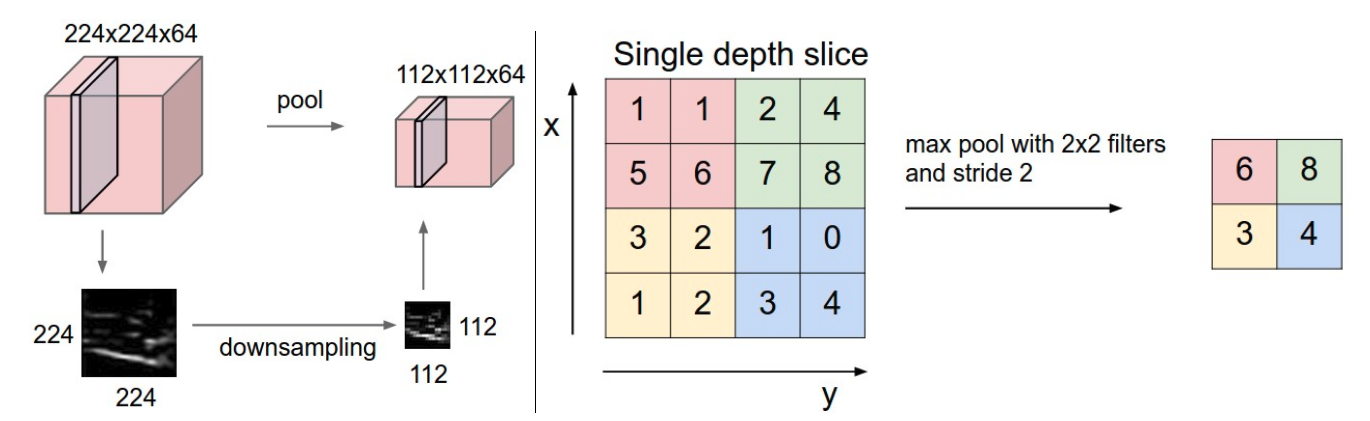
\includegraphics{./img/maxpooling.png}

}

\caption{\label{fig-maxpooling}Max-pooling layer. Source: Stanford's
CS231n course \url{http://cs231n.github.io/convolutional-networks}}

\end{figure}

A convolutional neural network is simply a sequence of convolutional
layers and max-pooling layers (sometime two convolutional layers are
applied in a row before max-pooling, as in VGG (Simonyan and Zisserman,
2015)), followed by a couple of fully-connected layers and a softmax
output layer. Figure~\ref{fig-alexnet} shows the architecture of
AlexNet, the winning architecture of the ImageNet challenge in 2012
(Krizhevsky et al., 2012).

\begin{figure}

{\centering 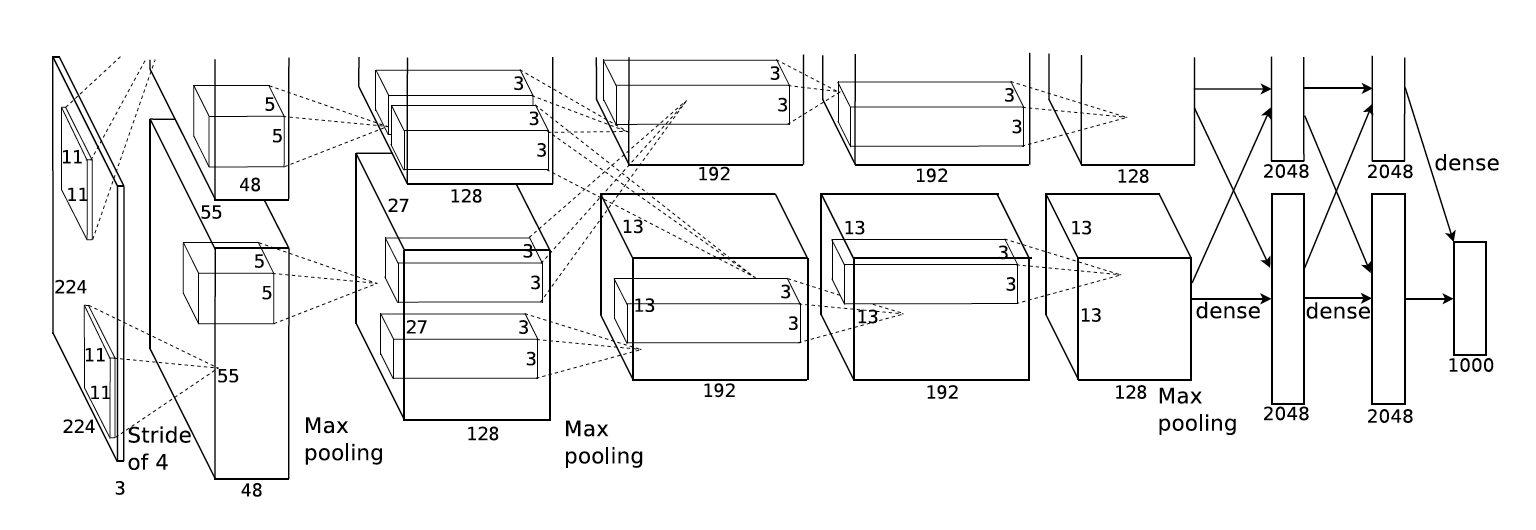
\includegraphics{./img/alexnet.png}

}

\caption{\label{fig-alexnet}Architecture of the AlexNet CNN. Taken from
Krizhevsky et al. (2012).}

\end{figure}

Many improvements have been proposed since 2012 (e.g.~ResNets (He et
al., 2015)) but the idea stays similar. Generally, convolutional and
max-pooling layers are alternated until the spatial dimensions are so
reduced (around 10x10) that they can be put into a single vector and fed
into a fully-connected layer. This is \textbf{NOT} the case in deep RL!
Contrary to object classification, spatial information is crucial in
deep RL: position of the ball, position of the body, etc. It matters
whether the ball is to the right or to the left of your paddle when you
decide how to move it. Max-pooling layers are therefore omitted and the
CNNs only consist of convolutional and fully-connected layers. This
greatly increases the number of weights in the networks, hence the
number of training examples needed to train the network. This is still
the main limitation of using CNNs in deep RL.

\hypertarget{recurrent-neural-networks}{%
\subsection{Recurrent neural networks}\label{recurrent-neural-networks}}

Feedforward neural networks learn to efficiently map static inputs
\(\mathbf{x}\) to outputs \(\mathbf{y}\) but have no memory or context:
the output at time \(t\) does not depend on the inputs at time \(t-1\)
or \(t-2\), only the one at time \(t\). This is problematic when dealing
with video sequences for example: if the task is to classify videos into
happy/sad, a frame by frame analysis is going to be inefficient (most
frames a neutral). Concatenating all frames in a giant input vector
would increase dramatically the complexity of the classifier and no
generalization can be expected.

Recurrent Neural Networks (RNN) are designed to deal with time-varying
inputs, where the relevant information to take a decision at time \(t\)
may have happened at different times in the past. The general structure
of a RNN is depicted on Figure~\ref{fig-rnn}:

\begin{figure}

{\centering 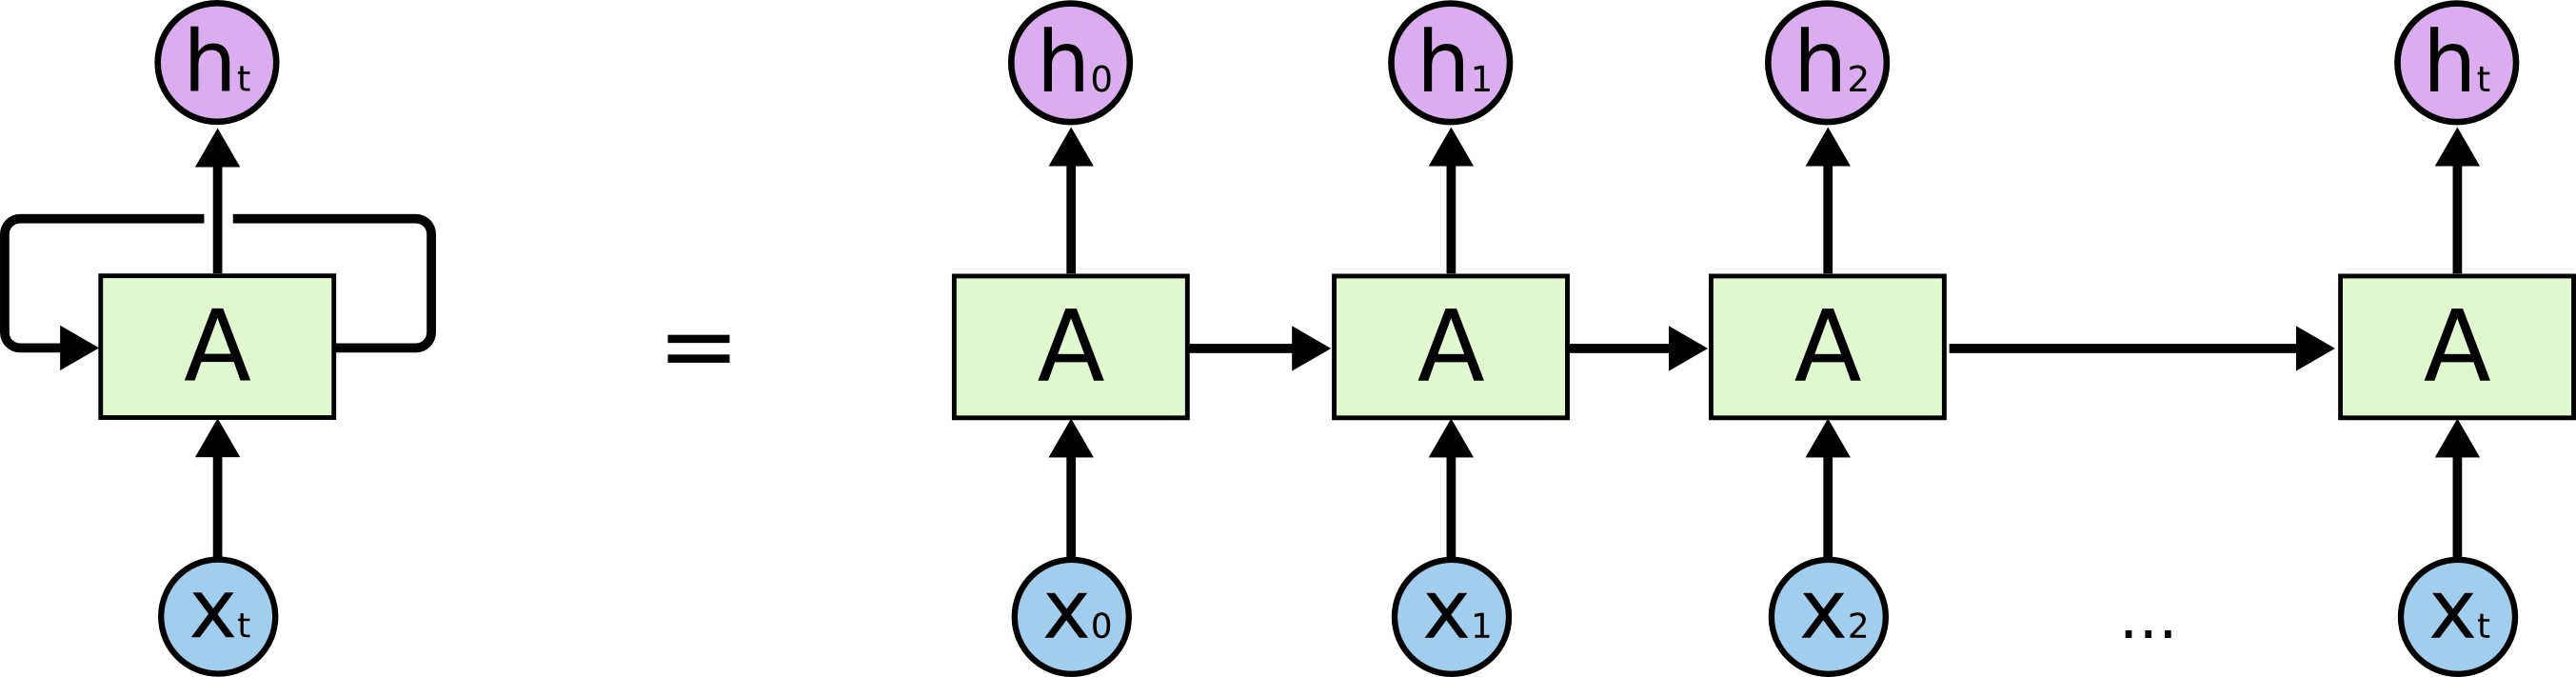
\includegraphics[width=0.9\textwidth,height=\textheight]{./img/RNN-unrolled.png}

}

\caption{\label{fig-rnn}Architecture of a RNN. Left: recurrent
architecture. Right: unrolled network, showing that a RNN is equivalent
to a deep network. Taken from
\url{http://colah.github.io/posts/2015-08-Understanding-LSTMs}.}

\end{figure}

The output \(\mathbf{h}_t\) of the RNN at time \(t\) depends on its
current input \(\mathbf{x}_t\), but also on its previous output
\(\mathbf{h}_{t-1}\), which, by recursion, depends on the whole history
of inputs \((x_0, x_1, \ldots, x_t)\).

\[
    \mathbf{h}_t = f(W_x \, \mathbf{x}_{t} + W_h \, \mathbf{h}_{t-1} + \mathbf{b})
\]

Once unrolled, a RNN is equivalent to a deep network, with \(t\) layers
of weights between the first input \(\mathbf{x}_0\) and the current
output \(\mathbf{h}_t\). The only difference with a feedforward network
is that weights are reused between two time steps / layers.
\textbf{Backpropagation though time} (BPTT) can be used to propagate the
gradient of the loss function backwards in time and learn the weights
\(W_x\) and \(W_h\) using the usual optimizer (SGD, Adam\ldots).

However, this kind of RNN can only learn short-term dependencies because
of the \textbf{vanishing gradient problem} (Hochreiter, 1991). When the
gradient of the loss function travels backwards from \(\mathbf{h}_t\) to
\(\mathbf{x}_0\), it will be multiplied \(t\) times by the recurrent
weights \(W_h\). If \(|W_h| > 1\), the gradient will explode with
increasing \(t\), while if \(|W_h| < 1\), the gradient will vanish to 0.

The solution to this problem is provided by \textbf{long short-term
memory networks} {[}LSTM;Hochreiter and Schmidhuber (1997){]}. LSTM
layers maintain additionally a state \(\mathbf{C}_t\) (also called
context or memory) which is manipulated by three learnable gates (input,
forget and output gates). As in regular RNNs, a \emph{candidate state}
\(\tilde{\mathbf{C}_t}\) is computed based on the current input and the
previous output:

\[
    \tilde{\mathbf{C}_t} = f(W_x \, \mathbf{x}_{t} + W_h \, \mathbf{h}_{t-1} + \mathbf{b})
\]

\begin{figure}

{\centering 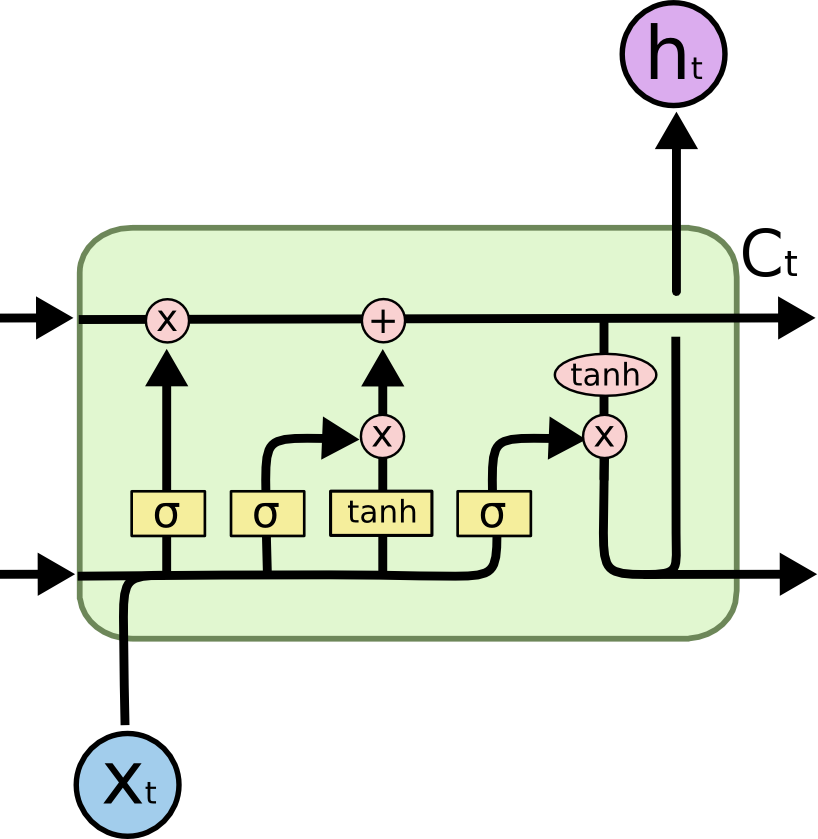
\includegraphics[width=0.4\textwidth,height=\textheight]{./img/LSTM.png}

}

\caption{\label{fig-lstm}Architecture of a LSTM layer. Taken from
\url{http://colah.github.io/posts/2015-08-Understanding-LSTMs}.}

\end{figure}

The activation function \(f\) is usually a tanh function. The input and
forget learn to decide how the candidate state should be used to update
the current state:

\begin{itemize}
\tightlist
\item
  The input gate decides which part of the candidate state
  \(\tilde{\mathbf{C}_t}\) will be used to update the current state
  \(\mathbf{C}_t\):
\end{itemize}

\[
    \mathbf{i}_t = \sigma(W^i_x \, \mathbf{x}_{t} + W^i_h \, \mathbf{h}_{t-1} + \mathbf{b}^i)
\]

The sigmoid activation function \(\sigma\) is used to output a number
between 0 and 1 for each neuron: 0 means the candidate state will not be
used at all, 1 means completely.

\begin{itemize}
\tightlist
\item
  The forget gate decides which part of the current state should be kept
  or forgotten:
\end{itemize}

\[
    \mathbf{f}_t = \sigma(W^f_x \, \mathbf{x}_{t} + W^f_h \, \mathbf{h}_{t-1} + \mathbf{b}^f)
\]

Similarly, 0 means that the corresponding element of the current state
will be erased, 1 that it will be kept.

Once the input and forget gates are computed, the current state can be
updated based on its previous value and the candidate state:

\[
   \mathbf{C}_t =  \mathbf{i}_t \odot \tilde{\mathbf{C}_t} + \mathbf{f}_t \odot \mathbf{C}_{t-1}
\]

where \(\odot\) is the element-wise multiplication.

\begin{itemize}
\tightlist
\item
  The output gate finally learns to select which part of the current
  state \(\mathbf{C}_t\) should be used to produce the current output
  \(\mathbf{h}_t\):
\end{itemize}

\[
    \mathbf{o}_t = \sigma(W^o_x \, \mathbf{x}_{t} + W^o_h \, \mathbf{h}_{t-1} + \mathbf{b}^o)
\]

\[
    \mathbf{h}_t = \mathbf{o}_t \odot \tanh \mathbf{C}_t
\]

The architecture may seem complex, but everything is differentiable:
backpropagation though time can be used to learn not only the input and
recurrent weights for the candidate state, but also the weights and and
biases of the gates. The main advantage of LSTMs is that they solve the
vanishing gradient problem: if the input at time \(t=0\) is important to
produce a response at time \(t\), the input gate will learn to put it
into the memory and the forget gate will learn to maintain in the
current state until it is not needed anymore. During this ``working
memory'' phase, the gradient is multiplied by exactly one as nothing
changes: the dependency can be learned with arbitrary time delays!

There are alternatives to the classical LSTM layer such as the gated
recurrent unit {[}GRU; Cho et al. (2014){]} or peephole connections
(Gers, 2001). See
\url{http://colah.github.io/posts/2015-08-Understanding-LSTMs},
\url{https://medium.com/mlreview/understanding-lstm-and-its-diagrams-37e2f46f1714}
or \url{http://blog.echen.me/2017/05/30/exploring-lstms/} for more
visual explanations of LSTMs and their variants.

RNNs are particularly useful for deep RL when considering POMDPs,
i.e.~partially observable problems. If an observation does not contain
enough information about the underlying state (e.g.~a single image does
not contain speed information), LSTM can integrate these observations
over time and learn to implicitly represent speed in its context vector,
allowing efficient policies to be learned.

\bookmarksetup{startatroot}

\hypertarget{value-based-methods}{%
\chapter{Value-based methods}\label{value-based-methods}}

\hypertarget{limitations-of-deep-neural-networks-for-function-approximation}{%
\section{Limitations of deep neural networks for function
approximation}\label{limitations-of-deep-neural-networks-for-function-approximation}}

The goal of value-based deep RL is to approximate the Q-value of each
possible state-action pair using a deep (convolutional) neural network.
As shown on Figure~\ref{fig-functionapprox2}, the network can either
take a state-action pair as input and return a single output value, or
take only the state as input and return the Q-value of all possible
actions (only possible if the action space is discrete), In both cases,
the goal is to learn estimates \(Q_\theta(s, a)\) with a NN with
parameters \(\theta\).

\begin{figure}

{\centering 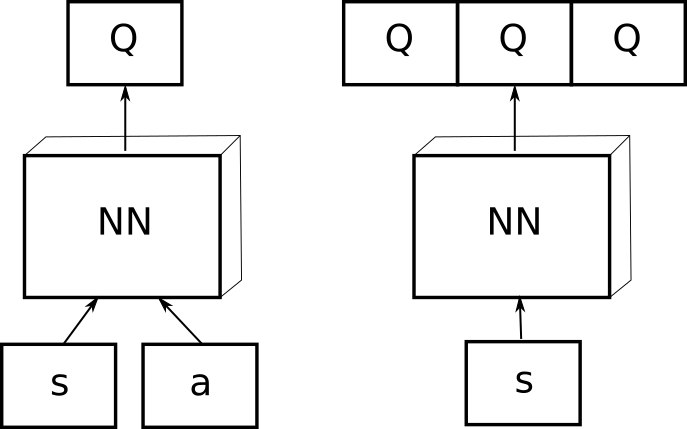
\includegraphics[width=0.6\textwidth,height=\textheight]{./img/functionapprox.png}

}

\caption{\label{fig-functionapprox2}Function approximators can either
associate a state-action pair \((s, a)\) to its Q-value (left), or
associate a state \(s\) to the Q-values of all actions possible in that
state (right).}

\end{figure}

When using Q-learning, we have already seen that the problem is a
regression problem, where the following mse loss function has to be
minimized:

\[
    \mathcal{L}(\theta) = \mathbb{E}_\pi[(r_t + \gamma \, \max_{a'} Q_\theta(s', a') - Q_\theta(s, a))^2]
\]

In short, we want to reduce the prediction error, i.e.~the mismatch
between the estimate of the value of an action \(Q_\theta(s, a)\) and
the real return, here approximated with
\(r(s, a, s') + \gamma \, \text{max}_{a'} Q_\theta(s', a')\).

We can compute this loss by gathering enough samples \((s, a, r, s')\)
(i.e.~single transitions), concatenating them randomly in minibatches,
and let the DNN learn to minimize the prediction error using
backpropagation and SGD, indirectly improving the policy. The following
pseudocode would describe the training procedure when gathering
transitions \textbf{online}, i.e.~when directly interacting with the
environment:

\begin{center}\rule{0.5\linewidth}{0.5pt}\end{center}

\begin{itemize}
\tightlist
\item
  Initialize value network \(Q_{\theta}\) with random weights.
\item
  Initialize empty minibatch \(\mathcal{D}\) of maximal size \(n\).
\item
  Observe the initial state \(s_0\).
\item
  for \(t \in [0, T_\text{total}]\):

  \begin{itemize}
  \tightlist
  \item
    Select the action \(a_t\) based on the behavior policy derived from
    \(Q_\theta(s_t, a)\) (e.g.~softmax).
  \item
    Perform the action \(a_t\) and observe the next state \(s_{t+1}\)
    and the reward \(r_{t+1}\).
  \item
    Predict the Q-value of the greedy action in the next state
    \(\max_{a'} Q_\theta(s_{t+1}, a')\)
  \item
    Store
    \((s_t, a_t, r_{t+1} + \gamma \, \max_{a'} Q_\theta(s_{t+1}, a'))\)
    in the minibatch.
  \item
    If minibatch \(\mathcal{D}\) is full:

    \begin{itemize}
    \tightlist
    \item
      Train the value network \(Q_{\theta}\) on \(\mathcal{D}\) to
      minimize
      \(\mathcal{L}(\theta) = \mathbb{E}_\mathcal{D}[(r(s, a, s') + \gamma \, \text{max}_{a'} Q_\theta(s', a') - Q_\theta(s, a))^2]\)
    \item
      Empty the minibatch \(\mathcal{D}\).
    \end{itemize}
  \end{itemize}
\end{itemize}

\begin{center}\rule{0.5\linewidth}{0.5pt}\end{center}

However, the definition of the loss function uses the mathematical
expectation operator \(E\) over all transitions, which can only be
approximated by \textbf{randomly} sampling the distribution (the MDP).
This implies that the samples concatenated in a minibatch should be
independent from each other (i.i.d). When gathering transitions online,
the samples are correlated: \((s_t, a_t, r_{t+1}, s_{t+1})\) will be
followed by \((s_{t+1}, a_{t+1}, r_{t+2}, s_{t+2})\), etc. When playing
video games, two successive frames will be very similar (a few pixels
will change, or even none if the sampling rate is too high) and the
optimal action will likely not change either (to catch the ball in pong,
you will need to perform the same action - going left - many times in a
row).

\textbf{Correlated inputs/outputs} are very bad for deep neural
networks: the DNN will overfit and fall into a very bad local minimum.
That is why stochastic gradient descent works so well: it randomly
samples values from the training set to form minibatches and minimize
the loss function on these uncorrelated samples (hopefully). If all
samples of a minibatch were of the same class (e.g.~zeros in MNIST), the
network would converge poorly. This is the first problem preventing an
easy use of deep neural networks as function approximators in RL.

The second major problem is the \textbf{non-stationarity} of the targets
in the loss function. In classification or regression, the desired
values \(\mathbf{t}\) are fixed throughout learning: the class of an
object does not change in the middle of the training phase.

\[
    \mathcal{L}(\theta) = - \mathbb{E}_{\mathbf{x}, \mathbf{t} \in \mathcal{D}}[ ||\mathbf{t} - \mathbf{y}||^2]
\]

In Q-learning, the target
\(r(s, a, s') + \gamma \, \max_{a'} Q_\theta(s', a')\) will change
during learning, as \(Q_\theta(s', a')\) depends on the weights
\(\theta\) and will hopefully increase as the performance improves. This
is the second problem of deep RL: deep NN are particularly bad on
non-stationary problems, especially feedforward networks. They
iteratively converge towards the desired value, but have troubles when
the target also moves (like a dog chasing its tail).

\hypertarget{deep-q-network-dqn}{%
\section{Deep Q-Network (DQN)}\label{deep-q-network-dqn}}

Mnih et al. (2015) (originally arXived in Mnih et al. (2013)) proposed
an elegant solution to the problems of correlated inputs/outputs and
non-stationarity inherent to RL. This article is a milestone of deep RL
and it is fair to say that it started or at least strongly renewed the
interest for deep RL.

The first idea proposed by Mnih et al. (2015) solves the problem of
correlated input/outputs and is actually quite simple: instead of
feeding successive transitions into a minibatch and immediately training
the NN on it, transitions are stored in a huge buffer called
\textbf{experience replay memory} (ERM) or \textbf{replay buffer} able
to store 100000 transitions. When the buffer is full, new transitions
replace the old ones. SGD can now randomly sample the ERM to form
minibatches and train the NN.

\begin{figure}

{\centering 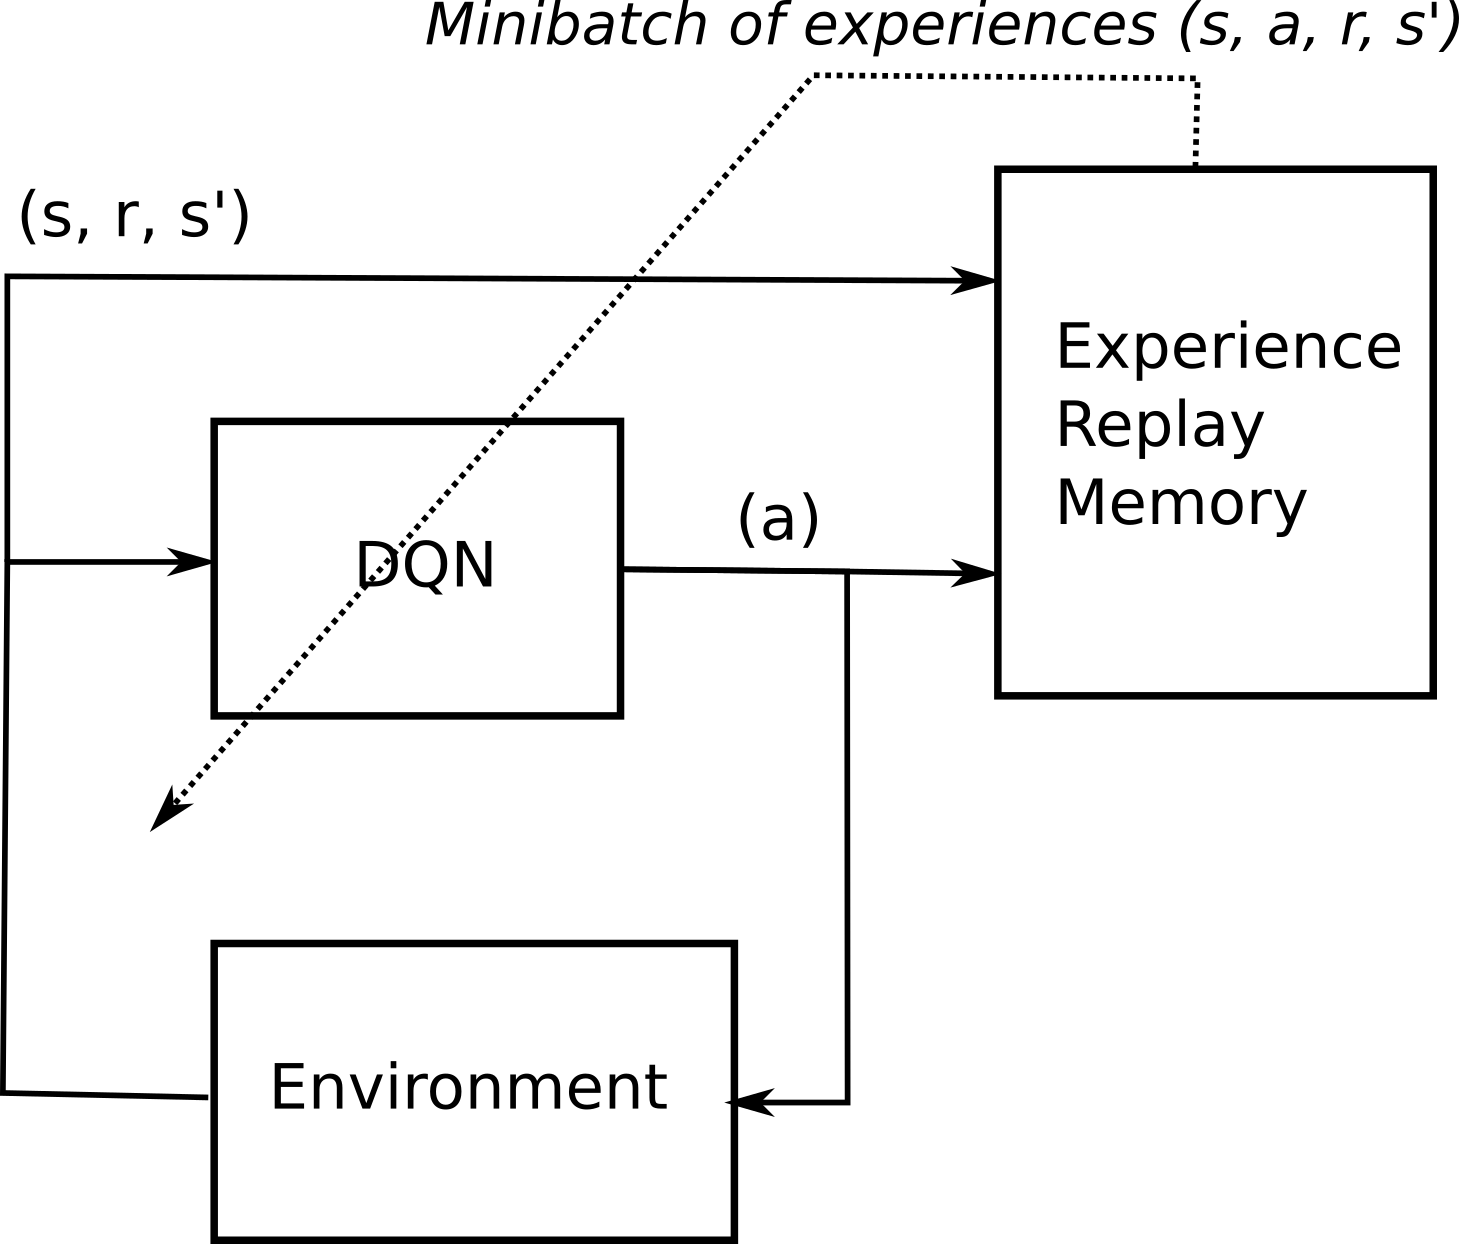
\includegraphics[width=0.4\textwidth,height=\textheight]{./img/ERM.png}

}

\caption{\label{fig-erm}Experience replay memory. Interactions with the
environment are stored in the ERM. Random minibatches are sampled from
it to train the DQN value network.}

\end{figure}

The second idea solves the non-stationarity of the targets
\(r(s, a, s') + \gamma \, \max_{a'} Q_\theta(s', a')\). Instead of
computing it with the current parameters \(\theta\) of the NN, they are
computed with an old version of the NN called the \textbf{target
network} with parameters \(\theta'\). The target network is updated only
infrequently (every thousands of iterations or so) with the learned
weights \(\theta\). As this target network does not change very often,
the targets stay constant for a long period of time, and the problem
becomes more stationary.

The resulting algorithm is called \textbf{Deep Q-Network (DQN)}. It is
summarized by the following pseudocode:

\begin{center}\rule{0.5\linewidth}{0.5pt}\end{center}

\begin{itemize}
\tightlist
\item
  Initialize value network \(Q_{\theta}\) with random weights.
\item
  Copy \(Q_{\theta}\) to create the target network \(Q_{\theta'}\).
\item
  Initialize experience replay memory \(\mathcal{D}\) of maximal size
  \(N\).
\item
  Observe the initial state \(s_0\).
\item
  for \(t \in [0, T_\text{total}]\):

  \begin{itemize}
  \tightlist
  \item
    Select the action \(a_t\) based on the behavior policy derived from
    \(Q_\theta(s_t, a)\) (e.g.~softmax).
  \item
    Perform the action \(a_t\) and observe the next state \(s_{t+1}\)
    and the reward \(r_{t+1}\).
  \item
    Store \((s_t, a_t, r_{t+1}, s_{t+1})\) in the experience replay
    memory.
  \item
    Every \(T_\text{train}\) steps:

    \begin{itemize}
    \tightlist
    \item
      Sample a minibatch \(\mathcal{D}_s\) randomly from
      \(\mathcal{D}\).
    \item
      For each transition \((s, a, r, s')\) in the minibatch:

      \begin{itemize}
      \tightlist
      \item
        Predict the Q-value of the greedy action in the next state
        \(\max_{a'} Q_{\theta'}(s', a')\) using the target network.
      \item
        Compute the target value
        \(y = r + \gamma \, \max_{a'} Q_{\theta'}(s', a')\).
      \end{itemize}
    \item
      Train the value network \(Q_{\theta}\) on \(\mathcal{D}_s\) to
      minimize
      \(\mathcal{L}(\theta) = \mathbb{E}_{\mathcal{D}_s}[(y - Q_\theta(s, a))^2]\)
    \end{itemize}
  \item
    Every \(T_\text{target}\) steps:

    \begin{itemize}
    \tightlist
    \item
      Update the target network with the trained value network:
      \(\theta' \leftarrow \theta\)
    \end{itemize}
  \end{itemize}
\end{itemize}

\begin{center}\rule{0.5\linewidth}{0.5pt}\end{center}

In this document, pseudocode will omit many details to simplify the
explanations (for example here, the case where a state is terminal - the
game ends - and the next state has to be chosen from the distribution of
possible starting states). Refer to the original publication for more
exact algorithms.

The first thing to notice is that experienced transitions are not
immediately used for learning, but simply stored in the ERM to be
sampled later. Due to the huge size of the ERM, it is even likely that
the recently experienced transition will only be used for learning
hundreds or thousands of steps later. Meanwhile, very old transitions,
generated using an initially bad policy, can be used to train the
network for a very long time.

The second thing is that the target network is not updated very often
(\(T_\text{target}=10000\)), so the target values are going to be wrong
a long time. More recent algorithms such as DDPG use a smoothed version
of the current weights, as proposed in Lillicrap et al. (2015):

\[
    \theta' = \tau \, \theta + (1-\tau) \, \theta'
\]

If this rule is applied after each step with a very small rate \(\tau\),
the target network will slowly track the learned network, but never be
the same.

These two facts make DQN extremely slow to learn: millions of
transitions are needed to obtain a satisfying policy. This is called the
\textbf{sample complexity}, i.e.~the number of transitions needed to
obtain a satisfying performance. DQN finds very good policies, but at
the cost of a very long training time.

DQN was initially applied to solve various Atari 2600 games. Video
frames were used as observations and the set of possible discrete
actions was limited (left/right/up/down, shoot, etc). The CNN used is
depicted on Figure~\ref{fig-dqn}. It has two convolutional layers, no
max-pooling, 2 fully-connected layer and one output layer representing
the Q-value of all possible actions in the games.

\begin{figure}

{\centering 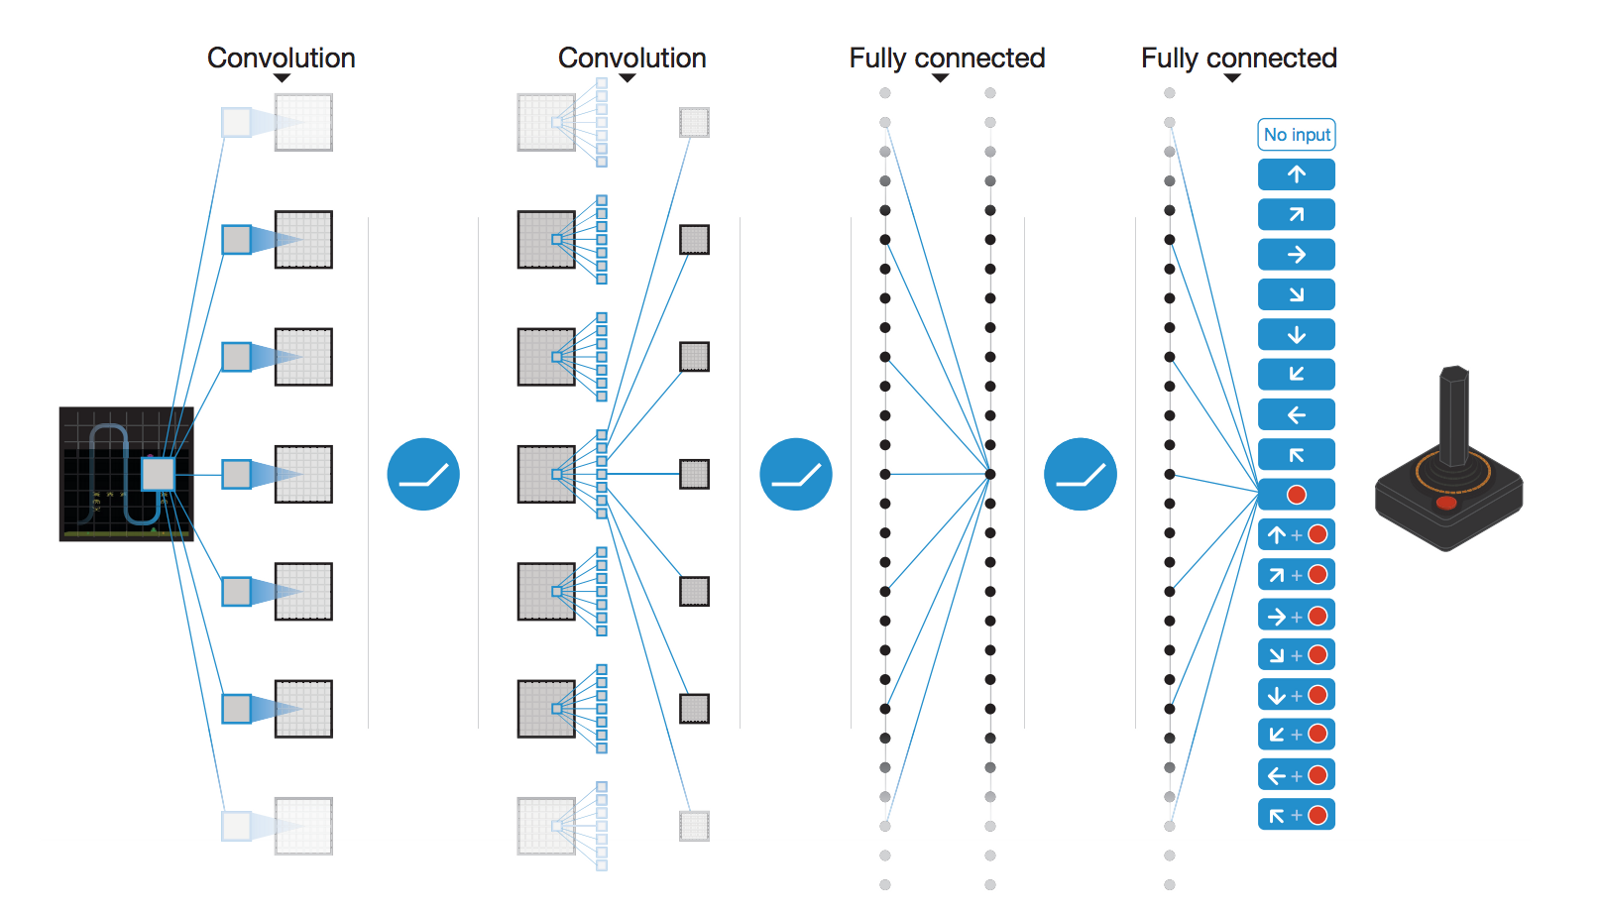
\includegraphics{./img/dqn.png}

}

\caption{\label{fig-dqn}Architecture of the CNN used in the original DQN
paper. Taken from Mnih et al. (2015).}

\end{figure}

The problem of partial observability is solved by concatenating the four
last video frames into a single tensor used as input to the CNN. The
convolutional layers become able through learning to extract the speed
information from it. Some of the Atari games (Pinball, Breakout) were
solved with a performance well above human level, especially when they
are mostly reactive. Games necessitating more long-term planning
(Montezuma' Revenge) were still poorly learned, though.

Beside being able to learn using delayed and sparse rewards in highly
dimensional input spaces, the true \emph{tour de force} of DQN is that
it was able to learn the 49 Atari games using the same architecture and
hyperparameters, showing the generality of the approach.

\hypertarget{double-dqn}{%
\section{Double DQN}\label{double-dqn}}

In DQN, the experience replay memory and the target network were
decisive in allowing the CNN to learn the tasks through RL. Their
drawback is that they drastically slow down learning and increase the
sample complexity. Additionally, DQN has stability issues: the same
network may not converge the same way in different runs. One first
improvement on DQN was proposed by van Hasselt et al. (2015) and called
\textbf{double DQN}.

The idea is that the target value
\(y = r(s, a, s') + \gamma \, \max_{a'} Q_{\theta'}(s', a')\) is
frequently over-estimating the true return because of the max operator.
Especially at the beginning of learning when Q-values are far from being
correct, if an action is over-estimated (\(Q_{\theta'}(s', a)\) is
higher that its true value) and selected by the target network as the
next greedy action, the learned Q-value \(Q_{\theta}(s, a)\) will also
become over-estimated, what will propagate to all previous actions on
the long-term. van Hasselt (2010) showed that this over-estimation is
inevitable in regular Q-learning and proposed \textbf{double learning}.

The idea is to train independently two value networks: one will be used
to find the greedy action (the action with the maximal Q-value), the
other to estimate the Q-value itself. Even if the first network choose
an over-estimated action as the greedy action, the other might provide a
less over-estimated value for it, solving the problem.

Applying double learning to DQN is particularly straightforward: there
are already two value networks, the trained network and the target
network. Instead of using the target network to both select the greedy
action in the next state and estimate its Q-value, here the trained
network \(\theta\) is used to select the greedy action
\(a^* = \text{argmax}_{a'} Q_\theta (s', a')\) while the target network
only estimates its Q-value. The target value becomes:

\[
    y = r(s, a, s') + \gamma \, Q_{\theta'}(s', \text{argmax}_{a'} Q_\theta (s', a'))
\]

This induces only a small modification of the DQN algorithm and
significantly improves its performance and stability:

\begin{center}\rule{0.5\linewidth}{0.5pt}\end{center}

\begin{itemize}
\tightlist
\item
  Every \(T_\text{train}\) steps:

  \begin{itemize}
  \tightlist
  \item
    Sample a minibatch \(\mathcal{D}_s\) randomly from \(\mathcal{D}\).
  \item
    For each transition \((s, a, r, s')\) in the minibatch:

    \begin{itemize}
    \tightlist
    \item
      Select the greedy action in the next state
      \(a^* = \text{argmax}_{a'} Q_\theta (s', a')\) using the trained
      network.
    \item
      Predict its Q-value \(Q_{\theta'}(s', a^*)\) using the target
      network.
    \item
      Compute the target value
      \(y = r + \gamma \, Q_{\theta'}(s', a*)\).
    \end{itemize}
  \end{itemize}
\end{itemize}

\begin{center}\rule{0.5\linewidth}{0.5pt}\end{center}

\hypertarget{prioritized-experience-replay}{%
\section{Prioritized experience
replay}\label{prioritized-experience-replay}}

Another drawback of the original DQN is that the experience replay
memory is sampled uniformly. Novel and interesting transitions are
selected with the same probability as old well-predicted transitions,
what slows down learning. The main idea of \textbf{prioritized
experience replay} (Schaul et al., 2015) is to order the transitions in
the experience replay memory in decreasing order of their TD error:

\[
    \delta = r(s, a, s') + \gamma \, Q_{\theta'}(s', \text{argmax}_{a'} Q_\theta (s', a')) - Q_\theta(s, a)
\]

and sample with a higher probability those surprising transitions to
form a minibatch. However, non-surprising transitions might become
relevant again after enough training, as the \(Q_\theta(s, a)\) change,
so prioritized replay has a softmax function over the TD error to ensure
``exploration'' of memorized transitions. This data structure has of
course a non-negligible computational cost, but accelerates learning so
much that it is worth it. See
\url{https://jaromiru.com/2016/11/07/lets-make-a-dqn-double-learning-and-prioritized-experience-replay/}
for a presentation of double DQN with prioritized replay.

\hypertarget{duelling-network}{%
\section{Duelling network}\label{duelling-network}}

The classical DQN architecture uses a single NN to predict directly the
value of all possible actions \(Q_\theta(s, a)\). The value of an action
depends on two factors:

\begin{itemize}
\tightlist
\item
  the value of the underlying state \(s\): in some states, all actions
  are bad, you lose whatever you do.
\item
  the interest of that action: some actions are better than others for a
  given state.
\end{itemize}

This leads to the definition of the \textbf{advantage} \(A^\pi(s,a)\) of
an action:

\begin{equation}\protect\hypertarget{eq-advantagefunction}{}{
    A^\pi(s, a) = Q^\pi(s, a) - V^\pi(s)
}\label{eq-advantagefunction}\end{equation}

The advantage of the optimal action in \(s\) is equal to zero: the
expected return in \(s\) is the same as the expected return when being
in \(s\) and taking \(a\), as the optimal policy will choose \(a\) in
\(s\) anyway. The advantage of all other actions is negative: they bring
less reward than the optimal action (by definition), so they are less
advantageous. Note that this is only true if your estimate of
\(V^\pi(s)\) is correct.

Baird (1993) has shown that it is advantageous to decompose the Q-value
of an action into the value of the state and the advantage of the action
(\emph{advantage updating}):

\[
    Q^\pi(s, a) = V^\pi(s) + A^\pi(s, a)
\]

If you already know that the value of a state is very low, you do not
need to bother exploring and learning the value of all actions in that
state, they will not bring much. Moreover, the advantage function has
\textbf{less variance} than the Q-values, which is a very good property
when using neural networks for function approximation. The variance of
the Q-values comes from the fact that they are estimated based on other
estimates, which themselves evolve during learning (non-stationarity of
the targets) and can drastically change during exploration (stochastic
policies). The advantages only track the \emph{relative} change of the
value of an action compared to its state, what is going to be much more
stable over time.

The range of values taken by the advantages is also much smaller than
the Q-values. Let's suppose we have two states with values -10 and 10,
and two actions with advantages 0 and -1 (it does not matter which one).
The Q-values will vary between -11 (the worst action in the worst state)
and 10 (the best action in the best state), while the advantage only
varies between -1 and 0. It is therefore going to be much easier for a
neural network to learn the advantages than the Q-values, as they are
theoretically not bounded.

\begin{figure}

{\centering 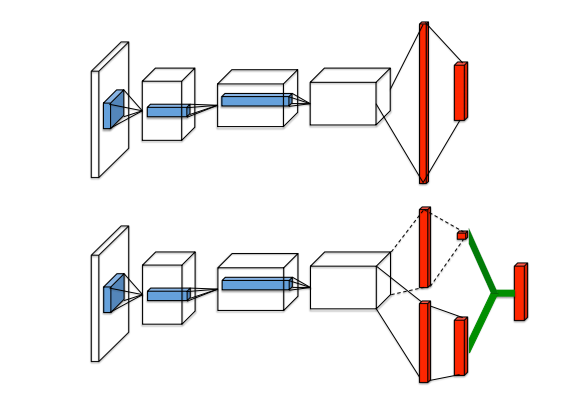
\includegraphics[width=0.6\textwidth,height=\textheight]{./img/duelling.png}

}

\caption{\label{fig-duelling}Duelling network architecture. Top:
classical feedforward architecture to predict Q-values. Bottom: Duelling
networks predicting state values and advantage functions to form the
Q-values. Taken from Wang et al. (2016).}

\end{figure}

Wang et al. (2016) incorporated the idea of \emph{advantage updating} in
a double DQN architecture with prioritized replay
(Figure~\ref{fig-duelling}). As in DQN, the last layer represents the
Q-values of the possible actions and has to minimize the mse loss:

\[
    \mathcal{L}(\theta) = \mathbb{E}_\pi([r(s, a, s') + \gamma \, Q_{\theta', \alpha', \beta'}(s', \text{argmax}_{a'} Q_{\theta, \alpha, \beta} (s', a')) - Q_{\theta, \alpha, \beta}(s, a)]^2)
\]

The difference is that the previous fully-connected layer is forced to
represent the value of the input state \(V_{\theta, \beta}(s)\) and the
advantage of each action \(A_{\theta, \alpha}(s, a)\) separately. There
are two separate sets of weights in the network, \(\alpha\) and
\(\beta\), to predict these two values, sharing representations from the
early convolutional layers through weights \(\theta\). The output layer
performs simply a parameter-less summation of both sub-networks:

\[
    Q_{\theta, \alpha, \beta}(s, a) = V_{\theta, \beta}(s) + A_{\theta, \alpha}(s, a)
\]

The issue with this formulation is that one could add a constant to
\(V_{\theta, \beta}(s)\) and substract it from
\(A_{\theta, \alpha}(s, a)\) while obtaining the same result. An easy
way to constrain the summation is to normalize the advantages, so that
the greedy action has an advantage of zero as expected:

\[
    Q_{\theta, \alpha, \beta}(s, a) = V_{\theta, \beta}(s) + (A_{\theta, \alpha}(s, a) - \max_a A_{\theta, \alpha}(s, a))
\]

By doing this, the advantages are still free, but the state value will
have to take the correct value. Wang et al. (2016) found that it is
actually better to replace the \(\max\) operator by the mean of the
advantages. In this case, the advantages only need to change as fast as
their mean, instead of having to compensate quickly for any change in
the greedy action as the policy improves:

\[
    Q_{\theta, \alpha, \beta}(s, a) = V_{\theta, \beta}(s) + (A_{\theta, \alpha}(s, a) - \frac{1}{|\mathcal{A}|} \sum_a A_{\theta, \alpha}(s, a))
\]

Apart from this specific output layer, everything works as usual,
especially the gradient of the mse loss function can travel backwards
using backpropagation to update the weights \(\theta\), \(\alpha\) and
\(\beta\). The resulting architecture outperforms double DQN with
prioritized replay on most Atari games, particularly games with
repetitive actions.

\hypertarget{rainbow-dqn}{%
\section{Rainbow DQN}\label{rainbow-dqn}}

As we have seen. the original formulation of DQN (Mnih et al., 2015) has
seen many improvements over the years.

\begin{itemize}
\tightlist
\item
  \textbf{Double DQN} (van Hasselt et al., 2015) separates the selection
  of the greedy action in the next state from its evaluation in order to
  prevent over-estimation of Q-values:
\end{itemize}

\[\mathcal{L}(\theta) = \mathbb{E}_\mathcal{D} [(r + \gamma \, Q_{\theta'}(s´, \text{argmax}_{a'} Q_{\theta}(s', a')) - Q_\theta(s, a))^2]\]

\begin{itemize}
\tightlist
\item
  \textbf{Prioritized Experience Replay} (Schaul et al., 2015) selects
  transitions from the ERM proportionally to their current TD error:
\end{itemize}

\[P(k) = \frac{(|\delta_k| + \epsilon)^\alpha}{\sum_k (|\delta_k| + \epsilon)^\alpha}\]

\begin{itemize}
\tightlist
\item
  \textbf{Dueling DQN} (Wang et al., 2016) splits learning of Q-values
  into learning of advantages and state values:
\end{itemize}

\[Q_\theta(s, a) = V_\alpha(s) + A_\beta(s, a)\]

\begin{itemize}
\tightlist
\item
  \textbf{Categorical DQN} (Bellemare et al., 2017) learns the
  distribution of returns instead of their expectation:
\end{itemize}

\[\mathcal{L}(\theta) = \mathbb{E}_{\mathcal{D}_s}[ - \mathbf{t}_k \, \log Z_\theta(s_k, a_k)]\]

\begin{itemize}
\tightlist
\item
  \textbf{n-step returns} (Sutton and Barto, 2017) reduce the bias of
  the estimation by taking the next \(n\) rewards into account, at the
  cost of a slightly higher variance.
\end{itemize}

\[\mathcal{L}(\theta) = \mathbb{E}_\mathcal{D} [(\sum_{k=1}^n r_{t+k} + \gamma \max_a Q_\theta(s_{t+n+1}, a) - Q_\theta(s_t, a_t))^2\]

\begin{itemize}
\tightlist
\item
  \textbf{Noisy DQN} (Fortunato et al., 2017) ensures exploration by
  adding noise to the parameters of the network instead of a softmax /
  \(\epsilon\)-greedy action selection over the Q-values.
\end{itemize}

All these improvements exceed the performance of vanilla DQN on most if
not all Atari game. But which ones are the most important?

Hessel et al. (2017) designed a \textbf{Rainbow DQN} integrating all
these improvements. Not only does the combined network outperform all
the DQN variants, but each of its components is important for its
performance as shown by ablation studies (apart from double learning and
duelling networks), see Figure~\ref{fig-rainbow}.

\begin{figure}

{\centering 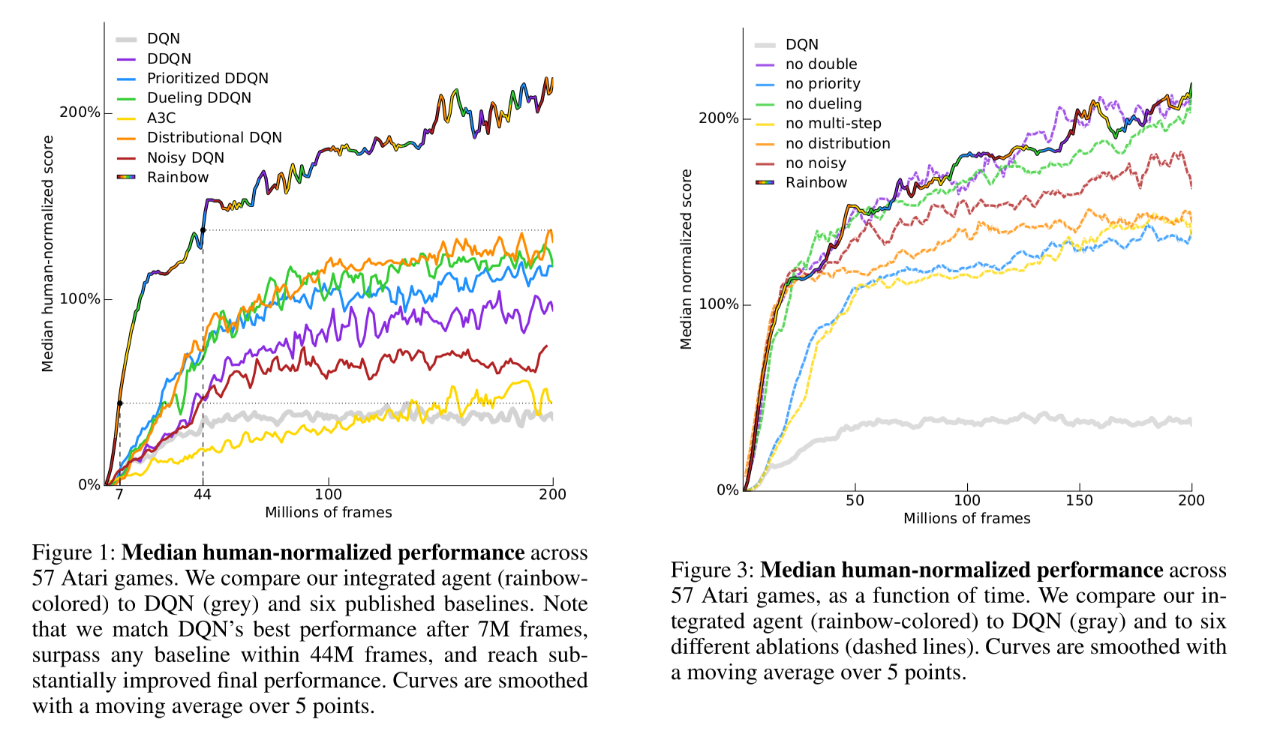
\includegraphics[width=0.9\textwidth,height=\textheight]{./img/rainbow.png}

}

\caption{\label{fig-rainbow}Performance of the Rainbow DQN compared to
other DQN variants (left) and ablation studies. Figures taken from
Hessel et al. (2017).}

\end{figure}

\hypertarget{distributed-dqn-gorila}{%
\section{Distributed DQN (GORILA)}\label{distributed-dqn-gorila}}

The main limitation of deep RL is the slowness of learning, which is
mainly influenced by two factors:

\begin{itemize}
\tightlist
\item
  the \textbf{sample complexity}, i.e.~the number of transitions needed
  to learn a satisfying policy.
\item
  the \textbf{online interaction} with the environment (states are
  visited one after the other).
\end{itemize}

The second factor is particularly critical in real-world applications
like robotics: physical robots evolve in real time, so the acquisition
speed of transitions will be limited. Even in simulation (video games,
robot emulators), the simulator might turn out to be much slower than
training the underlying neural network. Google Deepmind proposed the
GORILA (General Reinforcement Learning Architecture) framework to speed
up the training of DQN networks using distributed actors and learners
(Nair et al., 2015). The framework is quite general and the distribution
granularity can change depending on the task.

\begin{figure}

{\centering 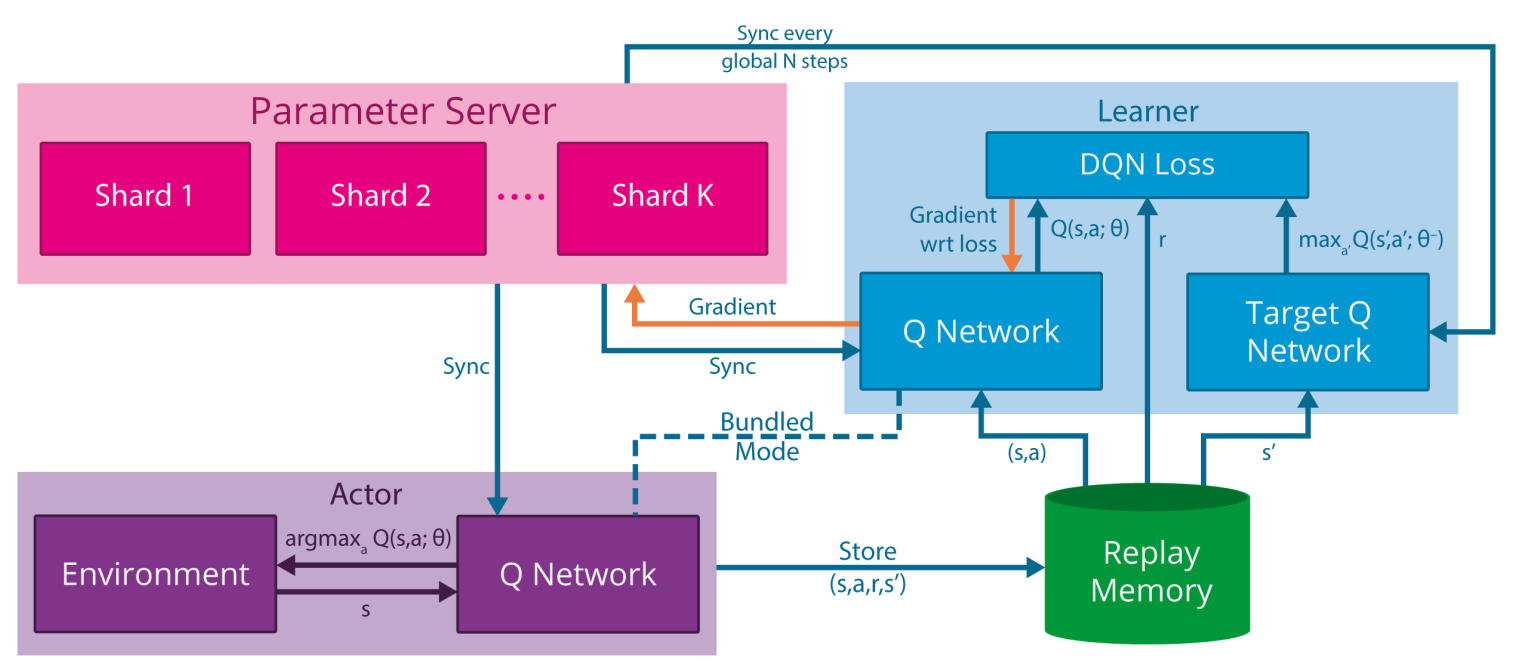
\includegraphics[width=0.9\textwidth,height=\textheight]{./img/gorila-global.png}

}

\caption{\label{fig-gorila}GORILA architecture. Multiple actors interact
with multiple copies of the environment and store their experiences in a
(distributed) experience replay memory. Multiple DQN learners sample
from the ERM and compute the gradient of the loss function w.r.t the
parameters \(\theta\). A master network (parameter server, possibly
distributed) gathers the gradients, apply weight updates and
synchronizes regularly both the actors and the learners with new
parameters. Taken from Nair et al. (2015).}

\end{figure}

In GORILA, multiple actors interact with the environment to gather
transitions. Each actor has an independent copy of the environment, so
they can gather \(N\) times more samples per second if there are \(N\)
actors. This is possible in simulation (starting \(N\) instances of the
same game in parallel) but much more complicated for real-world systems
(but see Gu et al. (2017) for an example where multiple identical robots
are used to gather experiences in parallel).

The experienced transitions are sent as in DQN to an experience replay
memory, which may be distributed or centralized. Multiple DQN learners
will then sample a minibatch from the ERM and compute the DQN loss on
this minibatch (also using a target network). All learners start with
the same parameters \(\theta\) and simply compute the gradient of the
loss function \(\frac{\partial \mathcal{L}(\theta)}{\partial \theta}\)
on the minibatch. The gradients are sent to a parameter server (a master
network) which uses the gradients to apply the optimizer (e.g.~SGD) and
find new values for the parameters \(\theta\). Weight updates can also
be applied in a distributed manner. This distributed method to train a
network using multiple learners is now quite standard in deep learning:
on multiple GPU systems, each GPU has a copy of the network and computes
gradients on a different minibatch, while a master network integrates
these gradients and updates the slaves.

The parameter server regularly updates the actors (to gather samples
with the new policy) and the learners (to compute gradients w.r.t the
new parameter values). Such a distributed system can greatly accelerate
learning, but it can be quite tricky to find the optimum number of
actors and learners (too many learners might degrade the stability) or
their update rate (if the learners are not updated frequently enough,
the gradients might not be correct).

Further variants of distributed DQN learning include Ape-X (Horgan et
al., 2018) and IMPALA (Espeholt et al., 2018). A similar idea is at the
core of the A3C algorithm, which is a policy gradient method.

\hypertarget{deep-recurrent-q-learning-drqn}{%
\section{Deep Recurrent Q-learning
(DRQN)}\label{deep-recurrent-q-learning-drqn}}

The Atari games used as a benchmark for value-based methods are
\textbf{partially observable MDPs} (POMDP), i.e.~a single frame does not
contain enough information to predict what is going to happen next
(e.g.~the speed and direction of the ball on the screen is not known).
In DQN, partial observability is solved by stacking four consecutive
frames and using the resulting tensor as an input to the CNN. if this
approach worked well for most Atari games, it has several limitations
(as explained in
\url{https://medium.com/emergent-future/simple-reinforcement-learning-with-tensorflow-part-6-partial-observability-and-deep-recurrent-q-68463e9aeefc}):

\begin{enumerate}
\def\labelenumi{\arabic{enumi}.}
\tightlist
\item
  It increases the size of the experience replay memory, as four video
  frames have to be stored for each transition.
\item
  It solves only short-term dependencies (instantaneous speeds). If the
  partial observability has long-term dependencies (an object has been
  hidden a long time ago but now becomes useful), the input to the
  neural network will not have that information. This is the main
  explanation why the original DQN performed so poorly on games
  necessitating long-term planning like Montezuma's revenge.
\end{enumerate}

Building on previous ideas from the Schmidhuber's group (Bakker, 2001;
Wierstra et al., 2007), Hausknecht and Stone (2015) replaced one of the
fully-connected layers of the DQN network by a LSTM layer while using
single frames as inputs. The resulting \textbf{deep recurrent
q-learning} (DRQN) network became able to solve POMDPs thanks to the
astonishing learning abilities of LSTMs: the LSTM layer learn to
remember which part of the sensory information will be useful to take
decisions later.

However, LSTMs are not a magical solution either. They are trained using
\emph{truncated BPTT}, i.e.~on a limited history of states. Long-term
dependencies exceeding the truncation horizon cannot be learned.
Additionally, all states in that horizon (i.e.~all frames) have to be
stored in the ERM to train the network, increasing drastically its size.
Despite these limitations, DRQN is a much more elegant solution to the
partial observability problem, letting the network decide which horizon
it needs to solve long-term dependencies.

\hypertarget{recurrent-replay-distributed-dqn-r2d2}{%
\section{Recurrent Replay Distributed DQN
(R2D2)}\label{recurrent-replay-distributed-dqn-r2d2}}

Kapturowski et al. (2019)

\hypertarget{other-variants-of-dqn}{%
\section{Other variants of DQN}\label{other-variants-of-dqn}}

\textbf{Average-DQN} (Anschel et al., 2016) proposes to increase the
stability and performance of DQN by replacing the single target network
(a copy of the trained network) by an average of the last parameter
values, in other words an average of many past target networks.

He et al. (2016) proposed \textbf{fast reward propagation} through
optimality tightening to speedup learning: when rewards are sparse, they
require a lot of episodes to propagate these rare rewards to all actions
leading to it. Their method combines immediate rewards (single steps)
with actual returns (as in Monte-Carlo) via a constrained optimization
approach.

\bookmarksetup{startatroot}

\hypertarget{policy-gradient-methods}{%
\chapter{Policy Gradient methods}\label{policy-gradient-methods}}

\textbf{Policy search} methods directly learn to estimate the policy
\(\pi_\theta\) with a parameterized function estimator. The goal of the
neural network is to maximize an objective function representing the
\emph{return} (sum of rewards, noted \(R(\tau)\) for simplicity) of the
trajectories \(\tau = (s_0, a_0, s_1, a_1, \ldots, s_T, a_T)\) selected
by the policy \(\pi_\theta\):

\[
    J(\theta) = \mathbb{E}_{\tau \sim \rho_\theta}[R(\tau)] = \mathbb{E}_{\tau \sim \rho_\theta}[\sum_{t=0}^T \gamma^t \, r(s_t, a_t, s_{t+1}) ]
\]

To maximize this objective function, the policy \(\pi_\theta\) should
only generate trajectories \(\tau\) associated with high returns
\(R(\tau)\) and avoid those with low return, which is exactly what we
want.

The objective function uses the mathematical expectation of the return
over all possible trajectories. The likelihood that a trajectory is
generated by the policy \(\pi_\theta\) is noted \(\rho_\theta(\tau)\)
and given by:

\begin{equation}\protect\hypertarget{eq-likelihood_trajectory}{}{
    \rho_\theta(\tau) = p_\theta(s_0, a_0, \ldots, s_T, a_T) = p_0 (s_0) \, \prod_{t=0}^T \pi_\theta(s_t, a_t) p(s_{t+1} | s_t, a_t)
}\label{eq-likelihood_trajectory}\end{equation}

\(p_0 (s_0)\) is the initial probability of starting in \(s_0\)
(independent from the policy) and \(p(s_{t+1} | s_t, a_t)\) is the
transition probability defining the MDP. Having the probability
distribution of the trajectories, we can expand the mathematical
expectation in the objective function:

\[
    J(\theta) = \int_\tau \rho_\theta (\tau) \, R(\tau) \, d\tau
\]

Monte-Carlo sampling could be used to estimate the objective function.
One basically would have to sample multiple trajectories \(\{\tau_i\}\)
and average the obtained returns:

\[
    J(\theta) \approx \frac{1}{N} \, \sum_{i=1}^N  R(\tau_i)
\]

However, this approach would suffer from several problems:

\begin{enumerate}
\def\labelenumi{\arabic{enumi}.}
\tightlist
\item
  The trajectory space is extremely huge, so one would need a lot of
  sampled trajectories to have a correct estimate of the objective
  function (\textbf{high variance}).
\item
  For stability reasons, only small changes can be made to the policy at
  each iteration, so it would necessitate a lot of episodes
  (\textbf{sample complexity}).
\item
  For continuing tasks (\(T = \infty\)), the return can not be estimated
  as the episode never ends.
\end{enumerate}

The policy search methods presented in this section are called
\textbf{policy gradient methods}. As we are going to apply gradient
ascent on the weights \(\theta\) in order to maximize \(J(\theta)\), all
we actually need is the gradient \(\nabla_\theta J(\theta)\) of the
objective function w.r.t the weights:

\[
    \nabla_\theta J(\theta) = \frac{\partial J(\theta)}{\partial \theta}
\]

Once a suitable estimation of this \textbf{policy gradient} is obtained,
gradient ascent is straightforward:

\[
    \theta \leftarrow \theta + \eta \, \nabla_\theta J(\theta)
\]

The rest of this section basically presents methods allowing to estimate
the policy gradient (REINFORCE, DPG) and to improve the sample
complexity. See
\url{http://www.scholarpedia.org/article/Policy_gradient_methods} for an
more detailed overview of policy gradient methods,
\url{https://lilianweng.github.io/lil-log/2018/04/08/policy-gradient-algorithms.html}
and \url{http://karpathy.github.io/2016/05/31/rl/} for excellent
tutorials from Lilian Weng and Andrej Karpathy. The article by Peters
and Schaal (2008) is also a good overview of policy gradient methods.

\hypertarget{reinforce}{%
\section{REINFORCE}\label{reinforce}}

\hypertarget{estimating-the-policy-gradient}{%
\subsection{Estimating the policy
gradient}\label{estimating-the-policy-gradient}}

Williams (1992) proposed a useful estimate of the policy gradient.
Considering that the return \(R(\tau)\) of a trajectory does not depend
on the parameters \(\theta\), one can simplify the policy gradient in
the following way:

\[
    \nabla_\theta J(\theta) = \nabla_\theta \int_\tau \rho_\theta (\tau) \, R(\tau) \, d\tau =  \int_\tau (\nabla_\theta \rho_\theta (\tau)) \, R(\tau) \, d\tau
\]

We now use the \textbf{log-trick}, a simple identity based on the fact
that:

\[
    \frac{d \log f(x)}{dx} = \frac{f'(x)}{f(x)}
\]

to rewrite the policy gradient of a single trajectory:

\[
    \nabla_\theta \rho_\theta (\tau) = \rho_\theta (\tau) \, \nabla_\theta \log \rho_\theta (\tau)
\]

The policy gradient becomes:

\[
    \nabla_\theta J(\theta) =  \int_\tau \rho_\theta (\tau) \, \nabla_\theta \log \rho_\theta (\tau) \, R(\tau) \, d\tau
\]

which now has the form of a mathematical expectation:

\[
    \nabla_\theta J(\theta) =  \mathbb{E}_{\tau \sim \rho_\theta}[ \nabla_\theta \log \rho_\theta (\tau) \, R(\tau) ]
\]

This means that we can obtain an estimate of the policy gradient by
simply sampling different trajectories \(\{\tau_i\}\) and averaging
\(\nabla_\theta \log \rho_\theta (\tau_i) \, R(\tau_i)\) (Monte-Carlo
sampling).

Let's now look further at how the gradient of the log-likelihood of a
trajectory \(\log \pi_\theta (\tau)\) look like. Through its definition
(Equation~\ref{eq-likelihood_trajectory}), the log-likelihood of a
trajectory is:

\begin{equation}\protect\hypertarget{eq-loglikelihood_trajectory}{}{
    \log \rho_\theta(\tau) = \log p_0 (s_0) + \sum_{t=0}^T \log \pi_\theta(s_t, a_t) + \sum_{t=0}^T \log p(s_{t+1} | s_t, a_t)
}\label{eq-loglikelihood_trajectory}\end{equation}

\(\log p_0 (s_0)\) and \(\log p(s_{t+1} | s_t, a_t)\) do not depend on
the parameters \(\theta\) (they are defined by the MDP), so the gradient
of the log-likelihood is simply:

\begin{equation}\protect\hypertarget{eq-gradloglikelihood_trajectory}{}{
    \nabla_\theta \log \rho_\theta(\tau) = \sum_{t=0}^T \nabla_\theta \log \pi_\theta(s_t, a_t)
}\label{eq-gradloglikelihood_trajectory}\end{equation}

\(\nabla_\theta \log \pi_\theta(s_t, a_t)\) is called the \textbf{score
function}.

This is the main reason why policy gradient algorithms are used: the
gradient is independent from the MDP dynamics, allowing
\textbf{model-free} learning. The policy gradient is then given by:

\[
    \nabla_\theta J(\theta) =  \mathbb{E}_{\tau \sim \rho_\theta}[\sum_{t=0}^T \nabla_\theta \log \pi_\theta(s_t, a_t) \, R(\tau) ] =  \mathbb{E}_{\tau \sim \rho_\theta}[ \sum_{t=0}^T \nabla_\theta \log \pi_\theta(s_t, a_t) \, (\sum_{t=0}^T \gamma^t r_{t+1})]
\]

Estimating the policy gradient now becomes straightforward using
Monte-Carlo sampling. The resulting algorithm is called the
\textbf{REINFORCE} algorithm (Williams, 1992):

\begin{center}\rule{0.5\linewidth}{0.5pt}\end{center}

\begin{itemize}
\item
  while not converged:

  \begin{itemize}
  \item
    Sample \(N\) trajectories \(\{\tau_i\}\) using the current policy
    \(\pi_\theta\) and observe the returns \(\{R(\tau_i)\}\).
  \item
    Estimate the policy gradient as an average over the trajectories:
  \end{itemize}

  \[
       \nabla_\theta J(\theta) \approx \frac{1}{N} \sum_{i=1}^N \sum_{t=0}^T \nabla_\theta \log \pi_\theta(s_t, a_t) \, R(\tau_i)
    \]

  \begin{itemize}
  \tightlist
  \item
    Update the policy using gradient ascent:
  \end{itemize}

  \[
        \theta \leftarrow \theta + \eta \, \nabla_\theta J(\theta)
    \]
\end{itemize}

\begin{center}\rule{0.5\linewidth}{0.5pt}\end{center}

While very simple, the REINFORCE algorithm does not work very well in
practice:

\begin{enumerate}
\def\labelenumi{\arabic{enumi}.}
\tightlist
\item
  The returns \(\{R(\tau_i)\}\) have a very high variance (as the
  Q-values in value-based methods), which is problematic for NNs.
\item
  It requires a lot of episodes to converge (sample inefficient).
\item
  It only works with \textbf{online} learning: trajectories must be
  frequently sampled and immediately used to update the policy.
\item
  The problem must be episodic (\(T\) finite).
\end{enumerate}

However, it has two main advantages:

\begin{enumerate}
\def\labelenumi{\arabic{enumi}.}
\tightlist
\item
  It is a \textbf{model-free} method, i.e.~one does not need to know
  anything about the MDP.
\item
  It also works on \textbf{partially observable} problems (POMDP): as
  the return is computed over complete trajectories, it does not matter
  if the states are not Markovian.
\end{enumerate}

The methods presented in this section basically try to solve the
limitations of REINFORCE (high variance, sample efficiency, online
learning) to produce efficient policy gradient algorithms.

\hypertarget{reducing-the-variance}{%
\subsection{Reducing the variance}\label{reducing-the-variance}}

The main problem with the REINFORCE algorithm is the \textbf{high
variance} of the policy gradient. This variance comes from the fact that
we learn stochastic policies (it is often unlikely to generate twice the
exact same trajectory) in stochastic environments (rewards are
stochastic, the same action in the same state may receive). Two
trajectories which are identical at the beginning will be associated
with different returns depending on the stochasticity of the policy, the
transition probabilities and the probabilistic rewards.

Consider playing a game like chess with always the same opening, and
then following a random policy. You may end up winning (\(R=1\)) or
losing (\(R=-1\)) with some probability. The initial actions of the
opening will receive a policy gradient which is sometimes positive,
sometimes negative: were these actions good or bad? Should they be
reinforced? In supervised learning, this would mean that the same image
of a cat will be randomly associated to the labels ``cat'' or ``dog''
during training: the NN will not like it.

In supervised learning, there is no problem of variance in the outputs,
as training sets are fixed. This is in contrary very hard to ensure in
deep RL and constitutes one of its main limitations. The only direct
solution is to sample enough trajectories and hope that the average will
be able to smooth the variance. The problem is even worse in the
following conditions:

\begin{itemize}
\tightlist
\item
  High-dimensional action spaces: it becomes difficult to sample the
  environment densely enough if many actions are possible.
\item
  Long horizons: the longer the trajectory, the more likely it will be
  unique.
\item
  Finite samples: if we cannot sample enough trajectories, the high
  variance can introduce a bias in the gradient, leading to poor
  convergence.
\end{itemize}

See
\url{https://medium.com/mlreview/making-sense-of-the-bias-variance-trade-off-in-deep-reinforcement-learning-79cf1e83d565}
for a nice explanation of the bias/variance trade-off in deep RL.

Another related problem is that the REINFORCE gradient is sensitive to
\textbf{reward scaling}. Let's consider a simple MDP where only two
trajectories \(\tau_1\) and \(\tau_2\) are possible. Depending on the
choice of the reward function, the returns may be different:

\begin{enumerate}
\def\labelenumi{\arabic{enumi}.}
\tightlist
\item
  \(R(\tau_1) = 1\) and \(R(\tau_2) = -1\)
\item
  \(R(\tau_1) = 3\) and \(R(\tau_2) = 1\)
\end{enumerate}

In both cases, the policy should select the trajectory \(\tau_1\).
However, the policy gradient for \(\tau_2\) will change its sign between
the two cases, although the problem is the same! What we want to do is
to maximize the returns, regardless the absolute value of the rewards,
but the returns are unbounded. Because of the non-stationarity of the
problem (the agent becomes better with training, so the returns of the
sampled trajectories will increase), the policy gradients will increase
over time, what is linked to the variance problem. Value-based methods
addressed this problem by using \textbf{target networks}, but it is not
a perfect solution (the gradients become biased).

A first simple but effective idea to solve both problems would be to
subtract the mean of the sampled returns from the returns:

\begin{center}\rule{0.5\linewidth}{0.5pt}\end{center}

\begin{itemize}
\item
  while not converged:

  \begin{itemize}
  \tightlist
  \item
    Sample \(N\) trajectories \(\{\tau_i\}\) using the current policy
    \(\pi_\theta\) and observe the returns \(\{R(\tau_i)\}\).
  \item
    Compute the mean return: \[
      \hat{R} = \frac{1}{N} \sum_{i=1}^N R(\tau_i)
      \]
  \item
    Estimate the policy gradient as an average over the trajectories: \[
     \nabla_\theta J(\theta) \approx \frac{1}{N} \sum_{i=1}^N \sum_{t=0}^T \nabla_\theta \log \pi_\theta(s_t, a_t) \, ( R(\tau_i) - \hat{R})
      \]
  \item
    Update the policy using gradient ascent: \[
      \theta \leftarrow \theta + \eta \, \nabla_\theta J(\theta)
      \]
  \end{itemize}
\end{itemize}

\begin{center}\rule{0.5\linewidth}{0.5pt}\end{center}

This obviously solves the reward scaling problem, and reduces the
variance of the gradients. But are we allowed to do this (i.e.~does it
introduce a bias to the gradient)? Williams (1992) showed that
subtracting a constant \(b\) from the returns still leads to an unbiased
estimate of the gradient:

\[
    \nabla_\theta J(\theta) =  \mathbb{E}_{\tau \sim \rho_\theta}[\nabla_\theta \log \rho_\theta (\tau) \, (R(\tau) -b) ]
\]

The proof is actually quite simple:

\[
    \mathbb{E}_{\tau \sim \rho_\theta}[\nabla_\theta \log \rho_\theta (\tau) \, b ] = \int_\tau \rho_\theta (\tau) \nabla_\theta \log \rho_\theta (\tau) \, b \, d\tau = \int_\tau \nabla_\theta  \rho_\theta (\tau) \, b \, d\tau = b \, \nabla_\theta \int_\tau \rho_\theta (\tau) \, d\tau =  b \, \nabla_\theta 1 = 0
\]

As long as the constant \(b\) does not depend on \(\theta\), the
estimator is unbiased. The resulting algorithm is called
\textbf{REINFORCE with baseline}. Williams (1992) has actually showed
that the best baseline (the one which also reduces the variance) is the
mean return weighted by the square of the gradient of the
log-likelihood:

\[
    b = \frac{\mathbb{E}_{\tau \sim \rho_\theta}[(\nabla_\theta \log \rho_\theta (\tau))^2 \, R(\tau)]}{\mathbb{E}_{\tau \sim \rho_\theta}[(\nabla_\theta \log \rho_\theta (\tau))^2]}
\]

but the mean reward actually work quite well. Advantage actor-critic
methods replace the constant \(b\) with an estimate of the value of each
state \(\hat{V}(s_t)\).

\hypertarget{policy-gradient-theorem}{%
\subsection{Policy Gradient theorem}\label{policy-gradient-theorem}}

Let's have another look at the REINFORCE estimate of the policy gradient
after sampling:

\[
   \nabla_\theta J(\theta) \approx \frac{1}{N} \sum_{i=1}^N \sum_{t=0}^T \nabla_\theta \log \pi_\theta(s_t, a_t) \, R(\tau_i) = \frac{1}{N} \sum_{i=1}^N (\sum_{t=0}^T \nabla_\theta \log \pi_\theta(s_t, a_t) ) \, (\sum_{t'=0}^T \gamma^{t'} \, r(s_{t'}, a_{t'}, s_{t'+1}) )
\]

For each transition \((s_t, a_t)\), the gradient of its log-likelihood
(\emph{score function}) \(\nabla_\theta \log \pi_\theta(s_t, a_t) )\) is
multiplied by the return of the whole episode
\(R(\tau) = \sum_{t'=0}^T \gamma^{t'} \, r(s_{t'}, a_{t'}, s_{t'+1})\).
However, the \textbf{causality principle} dictates that the reward
received at \(t=0\) does not depend on actions taken in the future, so
we can simplify the return for each transition:

\[
 \nabla_\theta J(\theta) \approx \frac{1}{N} \sum_{i=1}^N (\sum_{t=0}^T \nabla_\theta \log \pi_\theta(s_t, a_t)  \, \sum_{t'=t}^T \gamma^{t'-t} \, r(s_{t'}, a_{t'}, s_{t'+1}) )
\]

The quantity
\(\hat{Q}(s_t, a_t) = \sum_{t'=t}^T \gamma^{t'-t} \, r(s_{t'}, a_{t'}, s_{t'+1})\)
is called the \textbf{reward to-go} from the transition \((s_t, a_t)\),
i.e.~the discounted sum of future rewards after that transition. Quite
obviously, the Q-value of that action is the mathematical expectation of
this reward to-go.

\begin{figure}

{\centering 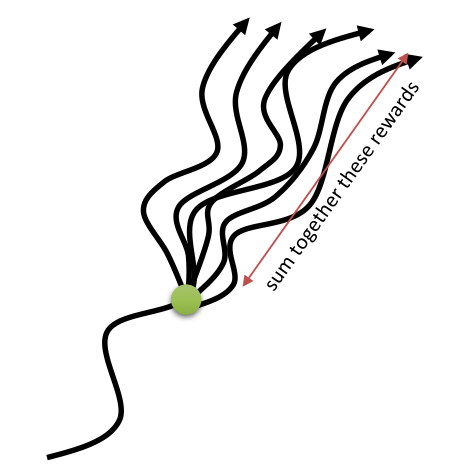
\includegraphics[width=0.3\textwidth,height=\textheight]{./img/rewardtogo.png}

}

\caption{\label{fig-rewardtogo}The reward to-go is the sum of rewards
gathered during a single trajectory after a transition \((s, a)\). The
Q-value of the action \((s, a)\) is the expectation of the reward to-go.
Taken from S. Levine's lecture
\url{http://rll.berkeley.edu/deeprlcourse/}.}

\end{figure}

\[
 \nabla_\theta J(\theta) \approx \frac{1}{N} \sum_{i=1}^N \sum_{t=0}^T \nabla_\theta \log \pi_\theta(s_t, a_t) \, \hat{Q}(s_t, a_t)
\]

Sutton et al. (1999) showed that the policy gradient can be estimated by
replacing the return of the sampled trajectory with the Q-value of each
action, what leads to the \textbf{policy gradient theorem}
(Equation~\ref{eq-policygradienttheorem}):

\begin{equation}\protect\hypertarget{eq-policygradienttheorem}{}{
    \nabla_\theta J(\theta) =  \mathbb{E}_{s \sim \rho_\theta, a \sim \pi_\theta}[\nabla_\theta \log \pi_\theta(s, a) \, Q^{\pi_\theta}(s, a)]
}\label{eq-policygradienttheorem}\end{equation}

where \(\rho_\theta\) is the distribution of states reachable under the
policy \(\pi_\theta\). Because the actual return \(R(\tau)\) is replaced
by its expectation \(Q^{\pi_\theta}(s, a)\), the policy gradient is now
a mathematical expectation over \textbf{single transitions} instead of
complete trajectories, allowing \textbf{bootstrapping} as in temporal
difference methods.

One clearly sees that REINFORCE is actually a special case of the policy
gradient theorem, where the Q-value of an action replaces the return
obtained during the corresponding trajectory.

The problem is of course that the true Q-value of the actions is as
unknown as the policy. However, Sutton et al. (1999) showed that it is
possible to estimate the Q-values with a function approximator
\(Q_\varphi(s, a)\) with parameters \(\varphi\) and obtain an unbiased
estimation:

\begin{equation}\protect\hypertarget{eq-policygradienttheoremapprox}{}{
    \nabla_\theta J(\theta) =  \mathbb{E}_{s \sim \rho_\theta, a \sim \pi_\theta}[\nabla_\theta \log \pi_\theta(s, a) \, Q_\varphi(s, a))]
}\label{eq-policygradienttheoremapprox}\end{equation}

Formally, the Q-value approximator must respect the Compatible Function
Approximation Theorem, which states that the value approximator must be
compatible with the policy
(\(\nabla_\varphi Q_\varphi(s, a) = \nabla_\theta \log \pi_\theta(s, a)\))
and minimize the mean-square error with the true Q-values
\(\mathbb{E}_{s \sim \rho^\pi, a \sim \pi_\theta} [(Q^{\pi_\theta}(s, a) - Q_\varphi(s, a))^2]\).
In the algorithms presented in this section, these conditions are either
met or neglected.

The resulting algorithm belongs to the \textbf{actor-critic} class, in
the sense that:

\begin{itemize}
\tightlist
\item
  The \textbf{actor} \(\pi_\theta(s, a)\) learns to approximate the
  policy by maximizing Equation~\ref{eq-policygradienttheoremapprox}.
\item
  The \textbf{critic} \(Q_\varphi(s, a)\) learns to estimate the policy
  by minimizing the mse with the true Q-values.
\end{itemize}

Figure~\ref{fig-actorcriticpolicy} shows the architecture of the
algorithm. The only problem left is to provide the critic with the true
Q-values.

\begin{figure}

{\centering 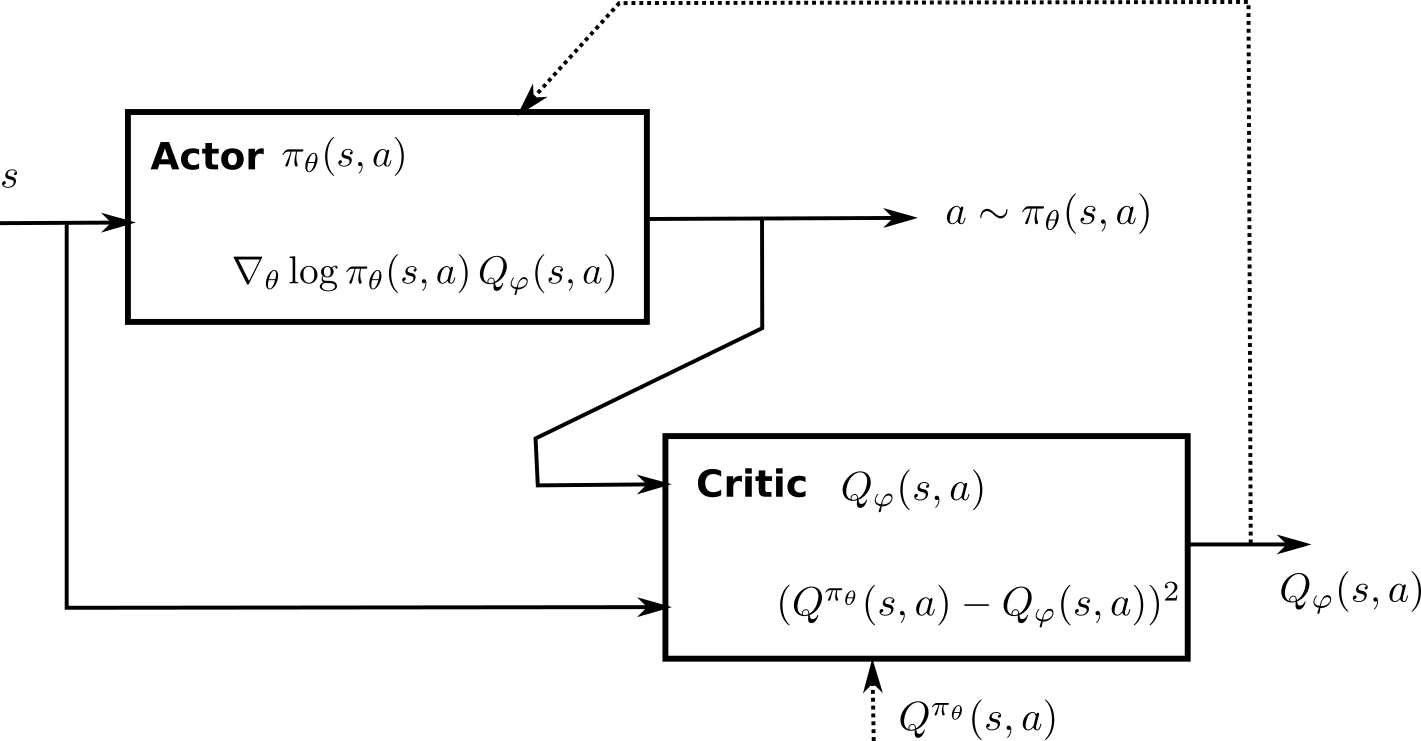
\includegraphics[width=0.8\textwidth,height=\textheight]{./img/policygradient.png}

}

\caption{\label{fig-actorcriticpolicy}Architecture of the policy
gradient (PG) method.}

\end{figure}

Most policy-gradient algorithms (A3C, DPPG, TRPO) are actor-critic
architectures. Some remarks already:

\begin{itemize}
\tightlist
\item
  Trajectories now appear only implicitly in the policy gradient, one
  can even sample single transitions. It should therefore be possible
  (with modifications) to do \textbf{off-policy learning}, for example
  with using importance sampling or a replay buffer of stored
  transitions as in DQN (see ACER). REINFORCE works strictly on-policy.
\item
  The policy gradient theorem suffers from the same \textbf{high
  variance} problem as REINFORCE. The different algorithms presented
  later are principally attempts to solve this problem and reduce the
  sample complexity: advantages, deterministic policies, natural
  gradients\ldots{}
\item
  The actor and the critic can be completely separated, or share some
  parameters.
\end{itemize}

\bookmarksetup{startatroot}

\hypertarget{advantage-actor-critic-methods}{%
\chapter{Advantage Actor-Critic
methods}\label{advantage-actor-critic-methods}}

The \emph{policy gradient theorem} provides an actor-critic architecture
able to learn parameterized policies. In comparison to REINFORCE, the
policy gradient depends on the Q-values of the actions taken during the
trajectory rather than on the obtained returns \(R(\tau)\). Quite
obviously, it will also suffer from the high variance of the gradient,
requiring the use of baselines. In this section, the baseline is
state-dependent and chosen equal to the value of the state \(V^\pi(s)\),
so the factor multiplying the log-likelihood of the policy is:

\[
    A^{\pi}(s, a) = Q^{\pi}(s, a) - V^\pi(s)
\]

which is the \textbf{advantage} of the action \(a\) in \(s\), as already
seen in \emph{duelling networks}.

Now the problem is that the critic would have to approximate two
functions: \(Q^{\pi}(s, a)\) and \(V^{\pi}(s)\). \textbf{Advantage
actor-critic} methods presented in this section (A2C, A3C, GAE)
approximate the advantage of an action:

\[
    \nabla_\theta J(\theta) =  \mathbb{E}_{s \sim \rho^\pi, a \sim \pi_\theta}[\nabla_\theta \log \pi_\theta(s, a) \, A_\varphi(s, a)]
\]

\(A_\varphi(s, a)\) is called the \textbf{advantage estimate} and should
be equal to the real advantage \emph{in expectation}.

Different methods could be used to compute the advantage estimate:

\begin{itemize}
\item
  \(A_\varphi(s, a) = R(s, a) - V_\varphi(s)\) is the \textbf{MC
  advantage estimate}, the Q-value of the action being replaced by the
  actual return.
\item
  \(A_\varphi(s, a) = r(s, a, s') + \gamma \, V_\varphi(s') - V_\varphi(s)\)
  is the \textbf{TD advantage estimate} or TD error.
\item
  \(A_\varphi(s, a) = \sum_{k=0}^{n-1} \gamma^{k} \, r_{t+k+1} + \gamma^n \, V_\varphi(s_{t+n+1}) - V_\varphi(s_t)\)
  is the \textbf{n-step advantage estimate}.
\end{itemize}

The most popular approach is the n-step advantage, which is at the core
of the methods A2C and A3C, and can be understood as a trade-off between
MC and TD. MC and TD advantages could be used as well, but come with the
respective disadvantages of MC (need for finite episodes, slow updates)
and TD (unstable). Generalized Advantage Estimation (GAE) takes another
interesting approach to estimate the advantage.

\emph{Note:} A2C is actually derived from the A3C algorithm presented
later, but it is simpler to explain it first. See
\url{https://blog.openai.com/baselines-acktr-a2c/} for an explanation of
the reasons. A good explanation of A2C and A3C with Python code is
available at
\url{https://cgnicholls.github.io/reinforcement-learning/2017/03/27/a3c.html}.

\hypertarget{advantage-actor-critic-a2c}{%
\subsection{Advantage Actor-Critic
(A2C)}\label{advantage-actor-critic-a2c}}

The first aspect of A2C is that it relies on n-step updating, which is a
trade-off between MC and TD:

\begin{itemize}
\tightlist
\item
  MC waits until the end of an episode to update the value of an action
  using the reward to-go (sum of obtained rewards) \(R(s, a)\).
\item
  TD updates immediately the action using the immediate reward
  \(r(s, a, s')\) and approximates the rest with the value of the next
  state \(V^\pi(s)\).
\item
  n-step uses the \(n\) next immediate rewards and approximates the rest
  with the value of the state visited \(n\) steps later.
\end{itemize}

\begin{equation}\protect\hypertarget{eq-a2c}{}{
    \nabla_\theta J(\theta) =  \mathbb{E}_{s_t \sim \rho^\pi, a_t \sim \pi_\theta}[\nabla_\theta \log \pi_\theta(s_t, a_t) \, ( \sum_{k=0}^{n-1} \gamma^{k} \, r_{t+k+1} + \gamma^n \, V_\varphi(s_{t+n+1}) - V_\varphi(s_t))]
}\label{eq-a2c}\end{equation}

TD can be therefore be seen as a 1-step algorithm. For sparse rewards
(mostly zero, +1 or -1 at the end of a game for example), this allows to
update the \(n\) last actions which lead to a win/loss, instead of only
the last one in TD, speeding up learning. However, there is no need for
finite episodes as in MC. In other words, n-step estimation ensures a
trade-off between bias (wrong updates based on estimated values as in
TD) and variance (variability of the obtained returns as in MC). An
alternative to n-step updating is the use of \emph{eligibility traces}
(see Sutton and Barto (1998)).

A2C has an actor-critic architecture (Figure~\ref{fig-a3c}):

\begin{itemize}
\tightlist
\item
  The actor outputs the policy \(\pi_\theta\) for a state \(s\), i.e.~a
  vector of probabilities for each action.
\item
  The critic outputs the value \(V_\varphi(s)\) of a state \(s\).
\end{itemize}

\begin{figure}

{\centering 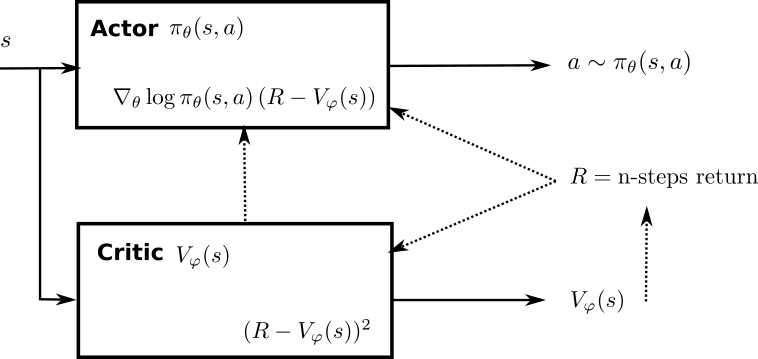
\includegraphics[width=0.7\textwidth,height=\textheight]{./img/a3c.png}

}

\caption{\label{fig-a3c}Advantage actor-critic architecture.}

\end{figure}

Having a computable formula for the policy gradient, the algorithm is
rather simple:

\begin{enumerate}
\def\labelenumi{\arabic{enumi}.}
\item
  Acquire a batch of transitions \((s, a, r, s')\) using the current
  policy \(\pi_\theta\) (either a finite episode or a truncated one).
\item
  For each state encountered, compute the discounted sum of the next
  \(n\) rewards \(\sum_{k=0}^{n} \gamma^{k} \, r_{t+k+1}\) and use the
  critic to estimate the value of the state encountered \(n\) steps
  later \(V_\varphi(s_{t+n+1})\).
\end{enumerate}

\[
    R_t = \sum_{k=0}^{n-1} \gamma^{k} \, r_{t+k+1} + \gamma^n \, V_\varphi(s_{t+n+1})
\]

\begin{enumerate}
\def\labelenumi{\arabic{enumi}.}
\setcounter{enumi}{2}
\tightlist
\item
  Update the actor using Equation~\ref{eq-a2c}.
\end{enumerate}

\[
    \nabla_\theta J(\theta) =  \sum_t \nabla_\theta \log \pi_\theta(s_t, a_t) \, (R_t - V_\varphi(s_t))
\]

\begin{enumerate}
\def\labelenumi{\arabic{enumi}.}
\setcounter{enumi}{3}
\tightlist
\item
  Update the critic to minimize the TD error between the estimated value
  of a state and its true value.
\end{enumerate}

\[
    \mathcal{L}(\varphi) = \sum_t (R_t - V_\varphi(s_t))^2
\]

\begin{enumerate}
\def\labelenumi{\arabic{enumi}.}
\setcounter{enumi}{4}
\tightlist
\item
  Repeat.
\end{enumerate}

This is not very different in essence from REINFORCE (sample
transitions, compute the return, update the policy), apart from the
facts that episodes do not need to be finite and that a critic has to be
learned in parallel. A more detailed pseudo-algorithm for a single A2C
learner is the following:

\begin{center}\rule{0.5\linewidth}{0.5pt}\end{center}

\begin{itemize}
\tightlist
\item
  Initialize the actor \(\pi_\theta\) and the critic \(V_\varphi\) with
  random weights.
\item
  Observe the initial state \(s_0\).
\item
  for \(t \in [0, T_\text{total}]\):

  \begin{itemize}
  \item
    Initialize empty episode minibatch.
  \item
    for \(k \in [0, n]\): \# Sample episode

    \begin{itemize}
    \tightlist
    \item
      Select a action \(a_k\) using the actor \(\pi_\theta\).
    \item
      Perform the action \(a_k\) and observe the next state \(s_{k+1}\)
      and the reward \(r_{k+1}\).
    \item
      Store \((s_k, a_k, r_{k+1})\) in the episode minibatch.
    \end{itemize}
  \item
    if \(s_n\) is not terminal: set \(R = V_\varphi(s_n)\) with the
    critic, else \(R=0\).
  \item
    Reset gradient \(d\theta\) and \(d\varphi\) to 0.
  \item
    for \(k \in [n-1, 0]\): \# Backwards iteration over the episode

    \begin{itemize}
    \tightlist
    \item
      Update the discounted sum of rewards \(R = r_k + \gamma \, R\)
    \item
      Accumulate the policy gradient using the critic: \[
        d\theta \leftarrow d\theta + \nabla_\theta \log \pi_\theta(s_k, a_k) \, (R - V_\varphi(s_k))
        \]
    \item
      Accumulate the critic gradient: \[
        d\varphi \leftarrow d\varphi + \nabla_\varphi (R - V_\varphi(s_k))^2
        \]
    \end{itemize}
  \item
    Update the actor and the critic with the accumulated gradients using
    gradient descent or similar: \[
      \theta \leftarrow \theta + \eta \, d\theta \qquad \varphi \leftarrow \varphi + \eta \, d\varphi
      \]
  \end{itemize}
\end{itemize}

\begin{center}\rule{0.5\linewidth}{0.5pt}\end{center}

Note that not all states are updated with the same horizon \(n\): the
last action encountered in the sampled episode will only use the last
reward and the value of the final state (TD learning), while the very
first action will use the \(n\) accumulated rewards. In practice it does
not really matter, but the choice of the discount rate \(\gamma\) will
have a significant influence on the results.

As many actor-critic methods, A2C performs online learning: a couple of
transitions are explored using the current policy, which is immediately
updated. As for value-based networks (e.g.~DQN), the underlying NN will
be affected by the correlated inputs and outputs: a single batch
contains similar states and action (e.g.~consecutive frames of a video
game). The solution retained in A2C and A3C does not depend on an
\emph{experience replay memory} as DQN, but rather on the use of
\textbf{multiple parallel actors and learners}.

The idea is depicted on Figure~\ref{fig-a3carchi} (actually for A3C, but
works with A2C). The actor and critic are stored in a global network.
Multiple instances of the environment are created in different parallel
threads (the \textbf{workers} or \textbf{actor-learners}). At the
beginning of an episode, each worker receives a copy of the actor and
critic weights from the global network. Each worker samples an episode
(starting from different initial states, so the episodes are
uncorrelated), computes the accumulated gradients and sends them back to
the global network. The global networks merges the gradients and uses
them to update the parameters of the policy and critic networks. The new
parameters are send to each worker again, until it converges.

\begin{center}\rule{0.5\linewidth}{0.5pt}\end{center}

\begin{itemize}
\tightlist
\item
  Initialize the actor \(\pi_\theta\) and the critic \(V_\varphi\) in
  the global network.
\item
  repeat:

  \begin{itemize}
  \tightlist
  \item
    for each worker \(i\) in \textbf{parallel}:

    \begin{itemize}
    \tightlist
    \item
      Get a copy of the global actor \(\pi_\theta\) and critic
      \(V_\varphi\).
    \item
      Sample an episode of \(n\) steps.
    \item
      Return the accumulated gradients \(d\theta_i\) and \(d\varphi_i\).
    \end{itemize}
  \item
    Wait for all workers to terminate.
  \item
    Merge all accumulated gradients into \(d\theta\) and \(d\varphi\).
  \item
    Update the global actor and critic networks.
  \end{itemize}
\end{itemize}

\begin{center}\rule{0.5\linewidth}{0.5pt}\end{center}

This solves the problem of correlated inputs and outputs, as each worker
explores different regions of the environment (one can set different
initial states in each worker, vary the exploration rate, etc), so the
final batch of transitions used for training the global networks is much
less correlated. The only drawback of this approach is that it has to be
possible to explore multiple environments in parallel. This is easy to
achieve in simulated environments (e.g.~video games) but much harder in
real-world systems like robots. A brute-force solution for robotics is
simply to buy enough robots and let them learn in parallel (Gu et al.,
2017).

\hypertarget{asynchronous-advantage-actor-critic-a3c}{%
\subsection{Asynchronous Advantage Actor-Critic
(A3C)}\label{asynchronous-advantage-actor-critic-a3c}}

\begin{figure}

{\centering 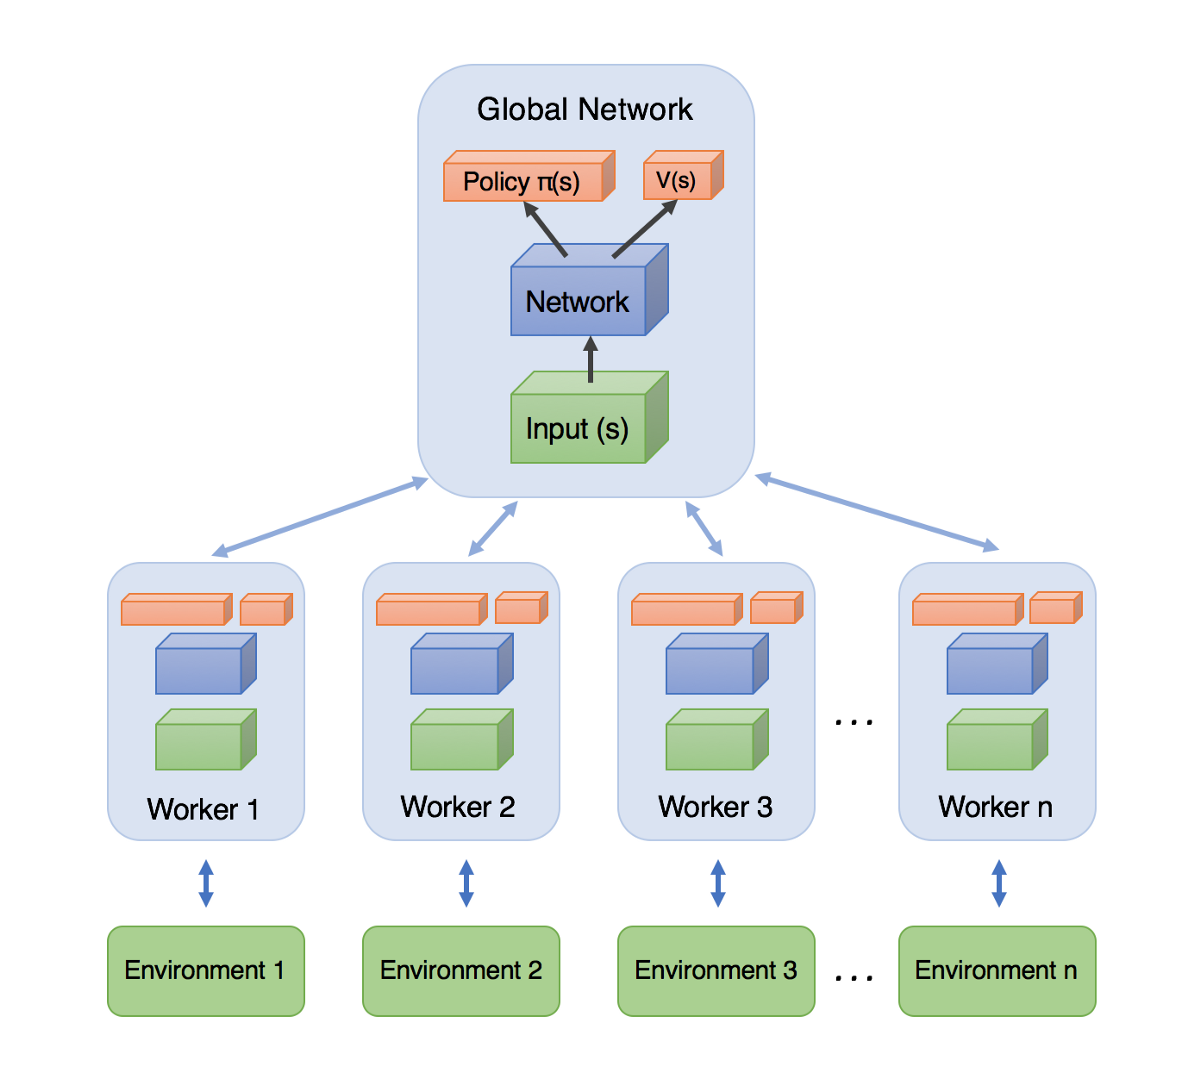
\includegraphics[width=0.7\textwidth,height=\textheight]{./img/A3C_architecture.png}

}

\caption{\label{fig-a3carchi}Architecture of A3C. A master network
interacts asynchronously with several workers, each having a copy of the
network and interacting with a separate environment. At the end of an
episode, the accumulated gradients are sent back to the master network,
and a new value of the parameters is sent to the workers. Taken from
\url{https://medium.com/emergent-future/simple-reinforcement-learning-with-tensorflow-part-8-asynchronous-actor-critic-agents-a3c-c88f72a5e9f2}.}

\end{figure}

Asynchronous Advantage Actor-Critic (A3C, Mnih et al., 2016) extends the
approach of A2C by removing the need of synchronization between the
workers at the end of each episode before applying the gradients. The
rationale behind this is that each worker may need different times to
complete its task, so they need to be synchronized. Some workers might
then be idle most of the time, what is a waste of resources. Gradient
merging and parameter updates are sequential operations, so no
significant speedup is to be expected even if one increases the number
of workers.

The solution retained in A3C is to simply skip the synchronization step:
each worker reads and writes the network parameters whenever it wants.
Without synchronization barriers, there is of course a risk that one
worker tries to read the network parameters while another writes them:
the obtained parameters would be a mix of two different networks.
Surprisingly, it does not matter: if the learning rate is small enough,
there is anyway not a big difference between two successive versions of
the network parameters. This kind of ``dirty'' parameter sharing is
called \emph{HogWild!} updating (Niu et al., 2011) and has been proven
to work under certain conditions which are met here.

The resulting A3C pseudocode is summarized here:

\begin{center}\rule{0.5\linewidth}{0.5pt}\end{center}

\begin{itemize}
\item
  Initialize the actor \(\pi_\theta\) and the critic \(V_\varphi\) in
  the global network.
\item
  for each worker \(i\) in \textbf{parallel}:

  \begin{itemize}
  \tightlist
  \item
    repeat:

    \begin{itemize}
    \tightlist
    \item
      Get a copy of the global actor \(\pi_\theta\) and critic
      \(V_\varphi\).
    \item
      Sample an episode of \(n\) steps.
    \item
      Compute the accumulated gradients \(d\theta_i\) and
      \(d\varphi_i\).
    \item
      Update the global actor and critic networks asynchronously
      (HogWild!).
    \end{itemize}
  \end{itemize}
\end{itemize}

\begin{center}\rule{0.5\linewidth}{0.5pt}\end{center}

The workers are fully independent: their only communication is through
the \textbf{asynchronous} updating of the global networks. This can lead
to very efficient parallel implementations: in the original A3C paper
(Mnih et al., 2016), they solved the same Atari games than DQN using 16
CPU cores instead of a powerful GPU, while achieving a better
performance in less training time (1 day instead of 8). The speedup is
almost linear: the more workers, the faster the computations, the better
the performance (as the policy updates are less correlated).

\hypertarget{entropy-regularization}{%
\subsubsection*{Entropy regularization}\label{entropy-regularization}}
\addcontentsline{toc}{subsubsection}{Entropy regularization}

An interesting addition in A3C is the way they enforce exploration
during learning. In actor-critic methods, exploration classically relies
on the fact that the learned policies are stochastic
(\textbf{on-policy}): \(\pi(s, a)\) describes the probability of taking
the action \(a\) in the state \(s\). In discrete action spaces, the
output of the actor is usually a softmax layer, ensuring that all
actions get a non-zero probability of being selected during training. In
continuous action spaces, the executed action is sampled from the output
probability distribution. However, this is often not sufficient and hard
to control.

In A3C, the authors added an \textbf{entropy regularization} term
(Williams and Peng, 1991) to the policy gradient update:

\begin{equation}\protect\hypertarget{eq-a3c_entropy}{}{
    \nabla_\theta J(\theta) =  \mathbb{E}_{s_t \sim \rho^\pi, a_t \sim \pi_\theta}[\nabla_\theta \log \pi_\theta(s_t, a_t) \, ( R_t - V_\varphi(s_t)) + \beta \, \nabla_\theta H(\pi_\theta(s_t))]
}\label{eq-a3c_entropy}\end{equation}

For discrete actions, the entropy of the policy for a state \(s_t\) is
simple to compute:
\(H(\pi_\theta(s_t)) = - \sum_a \pi_\theta(s_t, a) \, \log \pi_\theta(s_t, a)\).
For continuous actions, replace the sum with an integral. It measures
the ``randomness'' of the policy: if the policy is fully deterministic
(the same action is systematically selected), the entropy is zero as it
carries no information. If the policy is completely random, the entropy
is maximal. Maximizing the entropy at the same time as the returns
improves exploration by forcing the policy to be as non-deterministic as
possible.

The parameter \(\beta\) controls the level of regularization: we do not
want the entropy to dominate either, as a purely random policy does not
bring much reward. If \(\beta\) is chosen too low, the entropy won't
play a significant role in the optimization and we may obtain a
suboptimal deterministic policy early during training as there was not
enough exploration. If \(\beta\) is too high, the policy will be random.
Entropy regularization adds yet another hyperparameter to the problem,
but can be really useful for convergence when adequately chosen.

\hypertarget{comparison-between-a3c-and-dqn}{%
\subsubsection*{Comparison between A3C and
DQN}\label{comparison-between-a3c-and-dqn}}
\addcontentsline{toc}{subsubsection}{Comparison between A3C and DQN}

\begin{enumerate}
\def\labelenumi{\arabic{enumi}.}
\tightlist
\item
  DQN uses an experience replay memory to solve the correlation of
  inputs/outputs problem, while A3C uses parallel actor-learners. If
  multiple copies of the environment are available, A3C should be
  preferred because the ERM slows down learning (very old transitions
  are still used for learning) and requires a lot of memory.
\item
  A3C is on-policy: the learned policy must be used to explore the
  environment. DQN is off-policy: a behavior policy can be used for
  exploration, allowing to guide externally which regions of the
  state-action space should be explored. Off-policy are often preferred
  when expert knowledge is available.
\item
  DQN has to use target networks to fight the non-stationarity of the
  Q-values. A3C uses state-values and advantages, which are much more
  stable over time than Q-values, so there is no need for target
  networks.
\item
  A3C can deal with continuous action spaces easily, as it uses a
  parameterized policy. DQN has to be strongly modified to deal with
  this problem.
\item
  Both can deal with POMDP by using LSTMs in the actor network: A3C
  (Mirowski et al., 2016; Mnih et al., 2016), DQN (Hausknecht and Stone,
  2015).
\end{enumerate}

\hypertarget{generalized-advantage-estimation-gae}{%
\subsection{Generalized Advantage Estimation
(GAE)}\label{generalized-advantage-estimation-gae}}

The different versions of the policy gradient seen so far take the form:

\[
    \nabla_\theta J(\theta) =  \mathbb{E}_{s_t \sim \rho^\pi, a_t \sim \pi_\theta}[\nabla_\theta \log \pi_\theta (s_t, a_t) \, \psi_t ]
\]

where:

\begin{itemize}
\item
  \(\psi_t = R_t\) is the \emph{REINFORCE} algorithm (MC sampling).
\item
  \(\psi_t = R_t - b\) is the \emph{REINFORCE with baseline} algorithm.
\item
  \(\psi_t = Q^\pi(s_t, a_t)\) is the \emph{policy gradient theorem}.
\item
  \(\psi_t = A^\pi(s_t, a_t)\) is the \emph{advantage actor critic}.
\item
  \(\psi_t = r_{t+1} + \gamma \, V^\pi(s_{t+1}) - V^\pi(s_t)\) is the
  \emph{TD actor critic}.
\item
  \(\psi_t = \sum_{k=0}^{n-1} \gamma^{k} \, r_{t+k+1} + \gamma^n \, V^\pi(s_{t+n+1}) - V^\pi(s_t)\)
  is the \emph{n-step algorithm} (A2C).
\end{itemize}

Generally speaking:

\begin{itemize}
\tightlist
\item
  the more \(\psi_t\) relies on real rewards (e.g.~\(R_t\)), the more
  the gradient will be correct on average (small bias), but the more it
  will vary (high variance). This increases the sample complexity: we
  need to average more samples to correctly estimate the gradient.
\item
  the more \(\psi_t\) relies on estimations (e.g.~the TD error), the
  more stable the gradient (small variance), but the more incorrect it
  is (high bias). This can lead to suboptimal policies, i.e.~local
  optima of the objective function.
\end{itemize}

This is the classical bias/variance trade-off in machine learning. The
n-step algorithm used in A2C is an attempt to mitigate between these
extrema. Schulman et al. (2015a) proposed the \textbf{Generalized
Advantage Estimate} (GAE) to further control the bias/variance
trade-off.

Let's define the n-step advantage:

\[
    A^{n}_t = \sum_{k=0}^{n-1} \gamma^{k} \, r_{t+k+1} + \gamma^n \, V^\pi(s_{t+n+1}) - V^\pi(s_t)
\]

It is easy to show recursively that it depends on the TD error
\(\delta_t = r_{t+1} + \gamma \, V^\pi(s_{t+1}) - V^\pi(s_t)\) of the
\(n\) next steps:

\[
    A^{n}_t = \sum_{l=0}^{n-1} \gamma^l \, \delta_{t+l}
\]

In other words, the prediction error over \(n\) steps is the
(discounted) sum of the prediction errors between two successive steps.
Now, what is the optimal value of \(n\)? GAE decides not to choose and
to simply average all n-step advantages and to weight them with a
discount parameter \(\lambda\). This defines the \textbf{Generalized
Advantage Estimator} \(A^{\text{GAE}(\gamma, \lambda)}_t\):

\[
    A^{\text{GAE}(\gamma, \lambda)}_t = (1-\lambda) \, \sum_{l=0}^\infty \lambda^l A^l_t = \sum_{l=0}^\infty (\gamma \lambda)^l \delta_{t+l}
\]

The GAE is the discounted sum of all n-step advantages. When
\(\lambda=0\), we have
\(A^{\text{GAE}(\gamma, 0)}_t = A^{0}_t = \delta_t\), i.e.~the TD
advantage (high bias, low variance). When \(\lambda=1\), we have (at the
limit) \(A^{\text{GAE}(\gamma, 1)}_t = R_t\), i.e.~the MC advantage (low
bias, high variance). Choosing the right value of \(\lambda\) between 0
and 1 allows to control the bias/variance trade-off.

\(\gamma\) and \(\lambda\) play different roles in GAE: \(\gamma\)
determines the scale or horizon of the value functions: how much future
rewards rewards are to be taken into account. The higher \(\gamma <1\),
the smaller the bias, but the higher the variance. Empirically, Schulman
et al. (2015a) found that small \(\lambda\) values introduce less bias
than \(\gamma\), so \(\lambda\) can be chosen smaller than \(\gamma\)
(which is typically 0.99).

The policy gradient for Generalized Advantage Estimation is therefore:

\[
    \nabla_\theta J(\theta) =  \mathbb{E}_{s_t \sim \rho^\pi, a_t \sim \pi_\theta}[\nabla_\theta \log \pi_\theta (s_t, a_t) \, \sum_{l=0}^\infty (\gamma \lambda)^l \delta_{t+l} ]
\]

Note that Schulman et al. (2015a) additionally use \emph{trust region
optimization} to stabilize learning and further reduce the bias, for now
just consider it is a better optimization method than gradient descent.
The GAE algorithm is summarized here:

\begin{center}\rule{0.5\linewidth}{0.5pt}\end{center}

\begin{itemize}
\tightlist
\item
  Initialize the actor \(\pi_\theta\) and the critic \(V_\varphi\) with
  random weights.
\item
  for \(t \in [0, T_\text{total}]\):

  \begin{itemize}
  \item
    Initialize empty minibatch.
  \item
    for \(k \in [0, n]\):

    \begin{itemize}
    \tightlist
    \item
      Select a action \(a_k\) using the actor \(\pi_\theta\).
    \item
      Perform the action \(a_k\) and observe the next state \(s_{k+1}\)
      and the reward \(r_{k+1}\).
    \item
      Store \((s_k, a_k, r_{k+1})\) in the minibatch.
    \end{itemize}
  \item
    for \(k \in [0, n]\):

    \begin{itemize}
    \tightlist
    \item
      Compute the TD error
      \(\delta_k = r_{k+1} + \gamma \, V_\varphi(s_{k+1}) - V_\varphi(s_k)\)
    \end{itemize}
  \item
    for \(k \in [0, n]\):

    \begin{itemize}
    \tightlist
    \item
      Compute the GAE advantage
      \(A^{\text{GAE}(\gamma, \lambda)}_k = \sum_{l=0}^\infty (\gamma \lambda)^l \delta_{k+l}\)
    \end{itemize}
  \item
    Update the actor using the GAE advantage and natural gradients
    (TRPO).
  \item
    Update the critic using natural gradients (TRPO)
  \end{itemize}
\end{itemize}

\begin{center}\rule{0.5\linewidth}{0.5pt}\end{center}

\hypertarget{stochastic-actor-critic-for-continuous-action-spaces}{%
\subsection{Stochastic actor-critic for continuous action
spaces}\label{stochastic-actor-critic-for-continuous-action-spaces}}

The actor-critic method presented above use \textbf{stochastic policies}
\(\pi_\theta(s, a)\) assigning parameterized probabilities of being
selecting to each \((s, a)\) pair.

\begin{itemize}
\item
  When the action space is discrete, the output layer of the actor is
  simply a \emph{softmax} layer with as many neurons as possible actions
  in each state, making sure the probabilities sum to one. It is then
  straightforward to sample an action from this layer.
\item
  When the action space is continuous (e.g.~the different joints of a
  robotic arm), one has to make an assumption on the underlying
  distribution. The actor learns the parameters of the distribution (for
  example the mean and variance of a Gaussian distribution) and the
  executed action is simply sampled from the parameterized distribution.
\end{itemize}

The most used distribution is the Gaussian distribution, leading to
\textbf{Gaussian policies}. In this case, the output of the actor is a
mean vector \(\mu_\theta(s)\) and possibly a variance vector
\(\sigma_\theta(s)\). The policy is then simply defined as:

\[
    \pi_\theta(s, a) = \frac{1}{\sqrt{2\pi\sigma^2_\theta(s)}} \, \exp -\frac{(a - \mu_\theta(s))^2}{2\sigma_\theta(s)^2}
\]

In order to use backpropagation on the policy gradient (i.e.~getting an
analytical form of the score function
\(\nabla_\theta \log \pi_\theta (s, a)\)), one can use the
\emph{re-parameterization trick} (Heess et al., 2015) by rewriting the
policy as:

\[
    a = \mu_\theta(s) + \sigma_\theta(s) \times \xi \qquad \text{where} \qquad \xi \sim \mathcal{N}(0,1)
\]

To select an action, we only need to sample \(\xi\) from the unit normal
distribution, multiply it by the standard deviation and add the mean. To
compute the score function, we use the following partial derivatives:

\[
    \nabla_\mu \log \pi_\theta (s, a) = \frac{a - \mu_\theta(s)}{\sigma_\theta(s)^2} \qquad \nabla_\sigma \log \pi_\theta (s, a) = \frac{(a - \mu_\theta(s))^2}{\sigma_\theta(s)^3} - \frac{1}{\sigma_\theta(s)}
\]

and use the chain rule to obtain the score function. The
\emph{re-parameterization trick} is a cool trick to apply
backpropagation on stochastic problems: it is for example used in the
variational auto-encoders {[}VAE;Kingma and Welling (2013){]}.

Depending on the problem, one could use: 1) a fixed \(\sigma\) for the
whole action space, 2) a fixed \(\sigma\) per DoF, 3) a learnable
\(\sigma\) per DoF (assuming all action dimensions to be mutually
independent) or even 4) a covariance matrix \(\Sigma\) when the action
dimensions are dependent.

One limitation of Gaussian policies is that their support is infinite:
even with a small variance, samples actions can deviate a lot (albeit
rarely) from the mean. This is particularly a problem when action must
have a limited range: the torque of an effector, the linear or angular
speed of a car, etc. Clipping the sampled action to minimal and maximal
values introduces a bias which can impair learning. Chou et al. (2017)
proposed to use \textbf{beta-distributions} instead of Gaussian ones in
the actor. Sampled values have a \([0,1]\) support, which can rescaled
to \([v_\text{min},v_\text{max}]\) easily. They show that beta policies
have less bias than Gaussian policies in most continuous problems.

\bookmarksetup{startatroot}

\hypertarget{off-policy-actor-critic}{%
\chapter{Off-policy Actor-Critic}\label{off-policy-actor-critic}}

Actor-critic architectures are generally \textbf{on-policy} algorithms:
the actions used to explore the environment must have been generated by
the actor, otherwise the feedback provided by the critic (the advantage)
will introduce a huge bias (i.e.~an error) in the policy gradient. This
comes from the definition of the policy gradient theorem:

\[
    \nabla_\theta J(\theta) =  \mathbb{E}_{s \sim \rho^\pi, a \sim \pi_\theta}[\nabla_\theta \log \pi_\theta(s, a) \, Q^{\pi_\theta}(s, a)]
\]

The state distribution \(\rho^\pi\) defines the ensemble of states that
can be visited using the actor policy \(\pi_\theta\). If, during
Monte-Carlo sampling of the policy gradient, the states \(s\) do not
come from this state distribution, the approximated policy gradient will
be wrong (high bias) and the resulting policy will be suboptimal.

The major drawback of on-policy methods is their sample complexity: it
is difficult to ensure that the \emph{``interesting''} regions of the
policy are actually discovered by the actor (see
Figure~\ref{fig-onlinepolicyexploration}). If the actor is initialized
in a flat region of the reward space (where there is not a lot of
rewards), policy gradient updates will only change slightly the policy
and it may take a lot of iterations until interesting policies are
discovered and fine-tuned.

\begin{figure}

{\centering 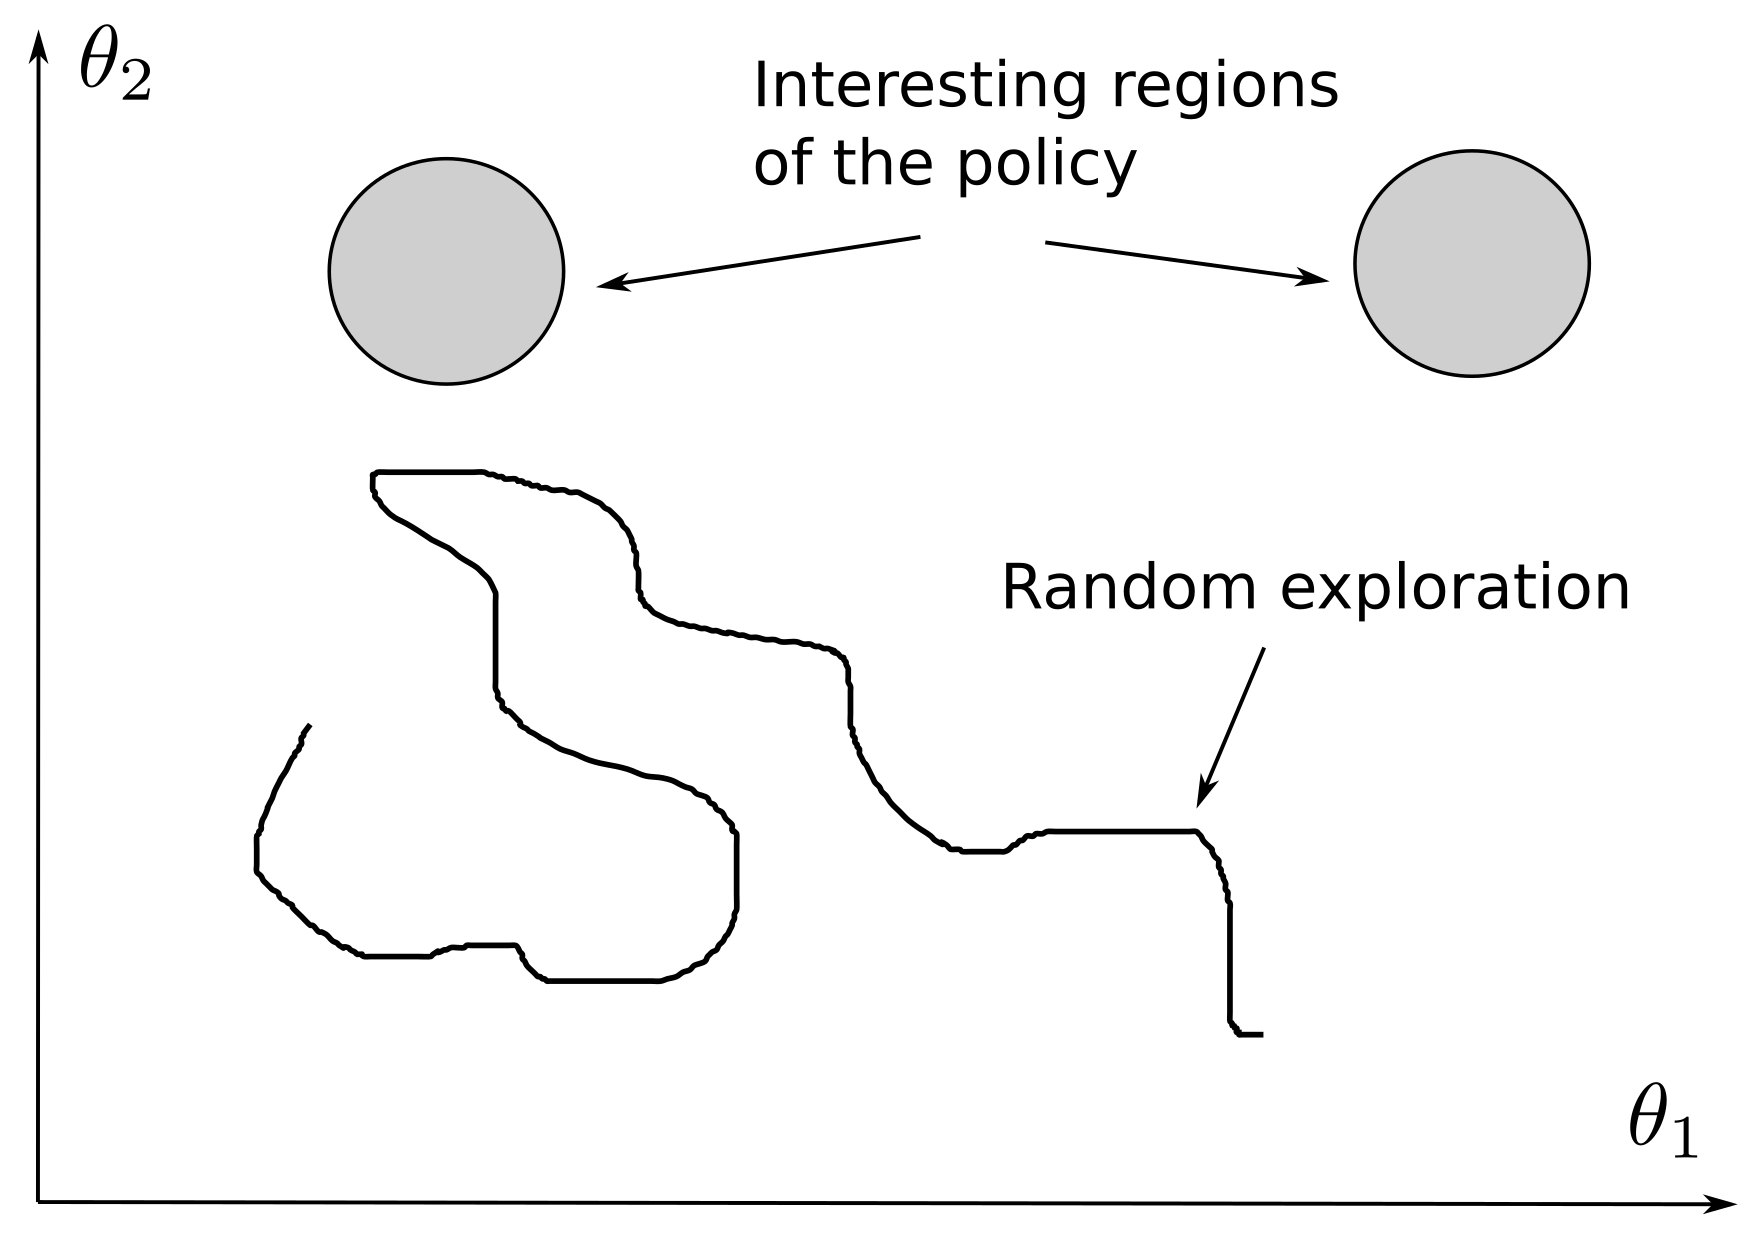
\includegraphics[width=0.5\textwidth,height=\textheight]{./img/onpolicyexploration.png}

}

\caption{\label{fig-onlinepolicyexploration}Illustration of the sample
complexity inherent to on-policy methods, where the actor has only two
parameters \(\theta_1\) and \(\theta_2\). If only very small regions of
the actor parameters are associated with high rewards, the policy might
wander randomly for a very long time before ``hitting''the interesting
regions.}

\end{figure}

The problem becomes even worse when the state or action spaces are
highly dimensional, or when rewards are sparse. Imagine the scenario
where you are searching for your lost keys at home (a sparse reward is
delivered only once you find them): you could spend hours trying
randomly each action at your disposal (looking in your jackets, on your
counter, but also jumping around, cooking something, watching TV\ldots)
until finally you explore the action ``look behind the curtains'' and
find them. (Note: with deep RL, you would even have to do that one
million times in order to allow gradient descent to train your
brain\ldots). If you had somebody telling you ``if I were you, I would
first search in your jackets, then on your counter and finally behind
the curtains, but forget about watching TV, you will never find anything
by doing that'', this would certainly reduce your exploration time.

This is somehow the idea behind \textbf{off-policy} algorithms: they use
a \textbf{behavior policy} \(b(s, a)\) to explore the environment and
train the \textbf{target policy} \(\pi(s, a)\) to reproduce the best
ones by estimating how good they are. This does not come without
caveats: if the behavior policy does not explore the optimal actions,
the target policy will likely not be able to find it by itself, except
by chance. But if the behavior policy is good enough, this can
drastically reduce the amount of exploration needed to obtain a
satisfying policy. Sutton and Barto (2017) noted that:

\emph{``On-policy methods are generally simpler and are considered
first. Off-policy methods require additional concepts and notation, and
because the data is due to a different policy, off-policy methods are
often of greater variance and are slower to converge.''}

The most famous off-policy method is Q-learning. The reason why it is
off-policy is that it does not use the next executed action
(\(a_{t+1}\)) to update the value of an action, but the greedy action in
the next state, which is independent from exploration:

\[
    \delta = r(s, a, s') + \gamma \, \max_{a'} Q^\pi(s', a') - Q^\pi(s, a)
\]

The only condition for Q-learning to work (in the tabular case) is that
the behavior policy \(b(s,a)\) must be able to explore actions which are
selected by the target policy:

\begin{equation}\protect\hypertarget{eq-qlearningcondition}{}{
    \pi(s, a) > 0 \rightarrow b(s, a) > 0
}\label{eq-qlearningcondition}\end{equation}

Actions which would be selected by the target policy should be selected
at least from time to time by the behavior policy in order to allow
their update: if the target policy thinks this action should be
executed, the behavior policy should try it to confirm or infirm this
assumption. In mathematical terms, there is an assumption of
\emph{coverage} of \(\pi\) by \(b\) (the support of \(b\) includes the
one of \(\pi\)).

There are mostly two ways to create the behavior policy:

\begin{enumerate}
\def\labelenumi{\arabic{enumi}.}
\item
  \emph{Use expert knowledge / human demonstrations}. Not all available
  actions should be explored: the programmer already knows they do not
  belong to the optimal policy. When an agent learns to play chess, for
  example, the behavior policy could consist of the moves typically
  played by human experts: if chess masters play this move, it is likely
  to be a good action, so it should be tried out, valued and possibly
  incorporated into the target policy (if it is indeed a good action,
  experts might be wrong). A similar idea was used to bootstrap early
  versions of AlphaGo (Silver et al., 2016a). In robotics, one could for
  example use ``classical'' engineering methods to control the
  exploration of the robot, while learning (hopefully) a better policy.
  It is also possible to perform \emph{imitation learning}, where the
  agent learns from human demonstrations (e.g. Levine and Koltun
  (2013)).
\item
  \emph{Derive it from the target policy}. In Q-learning, the target
  policy can be \textbf{deterministic}, i.e.~always select the greedy
  action (with the maximum Q-value). The behavior policy can be derived
  from the target policy by making it \emph{\(\epsilon\)-soft}, for
  example using a \(\epsilon\)-greedy or softmax action selection scheme
  on the Q-values learned by the target policy.
\end{enumerate}

The second option allows to control the level of exploration during
learning (by controlling \(\epsilon\) or the softmax temperature) while
making sure that the target policy (the one used in production) is
deterministic and optimal. It furthermore makes sure that
Equation~\ref{eq-qlearningcondition} is respected: the greedy action of
the target policy always has a non-zero probability of being selected by
an \(\epsilon\)-greedy or softmax action selection. This is harder to
ensure using expert knowledge.

Q-learning methods such as DQN use this second option. The target policy
in DQN is actually a greedy policy with respect to the Q-values
(i.e.~the action with the maximum Q-value will be deterministically
chosen), but an \(\epsilon\)-soft behavior policy is derived from it to
ensure exploration. This explains now the following comment in the
description of the DQN algorithm:

\begin{itemize}
\tightlist
\item
  Select the action \(a_t\) based on the behavior policy derived from
  \(Q_\theta(s_t, a)\) (e.g.~softmax).
\end{itemize}

Off-policy learning furthermore allows the use of an \textbf{experience
replay memory}: in this case, the transitions used for training the
target policy were generated by an older version of it (sometimes much
older). Only off-policy methods can work with replay buffers. A3C is for
example on-policy: it relies on multiple parallel learners to fight
against the correlation of inputs and outputs.

\hypertarget{importance-sampling}{%
\subsection{Importance sampling}\label{importance-sampling}}

Off-policy methods learn a target policy \(\pi(s,a)\) while exploring
with a behavior policy \(b(s,a)\). The environment is sampled using the
behavior policy to form estimates of the state or action values (for
value-based methods) or of the policy gradient (for policy gradient
methods). But is it mathematically correct?

In policy gradient methods, we want to maximize the expected return of
trajectories:

\[
    J(\theta) = \mathbb{E}_{\tau \sim \rho_\theta}[R(\tau)] = \int_\tau \rho_\theta(\tau) \, R(\tau) \, d\tau \approx \frac{1}{N} \sum_{i=1}^N R(\tau_i)
\]

where \(\rho_\theta\) is the distribution of trajectories \(\tau\)
generated by the \textbf{target} policy \(\pi_\theta\). Mathematical
expectations can be approximating by an average of enough samples of the
estimator (Monte-Carlo). In policy gradient, we estimate the gradient,
but let's consider we sample the objective function for now. If we use a
behavior policy to generate the trajectories, what we are actually
estimating is:

\[
    \hat{J}(\theta) = \mathbb{E}_{\tau \sim \rho_b}[R(\tau)] = \int_\tau \rho_b(\tau) \, R(\tau) \, d\tau
\]

where \(\rho_b\) is the distribution of trajectories generated by the
\textbf{behavior} policy. In the general case, there is no reason why
\(\hat{J}(\theta)\) should be close from \(J(\theta)\), even when taking
their gradient.

\textbf{Importance sampling} is a classical statistical method used to
estimate properties of a distribution (here the expected return of the
trajectories of the target policy) while only having samples generated
from a different distribution (here the trajectories of the behavior
policy). See for example
\url{https://statweb.stanford.edu/~owen/mc/Ch-var-is.pdf} and
\url{http://timvieira.github.io/blog/post/2014/12/21/importance-sampling}
for more generic explanations.

The trick is simply to rewrite the objective function as:

\[
\begin{aligned}
    J(\theta) & = \mathbb{E}_{\tau \sim \rho_\theta}[R(\tau)]  \\
              & = \int_\tau \rho_\theta(\tau) \, R(\tau) \, d\tau \\
              & = \int_\tau \frac{\rho_b(\tau)}{\rho_b(\tau)} \, \rho_\theta(\tau) \, R(\tau) \, d\tau \\
              & = \int_\tau \rho_b(\tau) \frac{\rho_\theta(\tau)}{\rho_b(\tau)} \, R(\tau) \, d\tau \\
              & = \mathbb{E}_{\tau \sim \rho_b}[\frac{\rho_\theta(\tau)}{\rho_b(\tau)} \, R(\tau)]  \\
\end{aligned}
\]

The ratio \(\frac{\rho_\theta(\tau)}{\rho_b(\tau)}\) is called the
\textbf{importance sampling weight} for the trajectory. If a trajectory
generated by \(b\) is associated with a lot of rewards \(R(\tau)\) (with
\(\rho_b(\tau)\) significantly high), the actor should learn to
reproduce that trajectory with a high probability \(\rho_\theta(\tau)\),
as its goal is to maximize \(J(\theta)\). Conversely, if the associated
reward is low (\(R(\tau)\approx 0\)), the target policy can forget about
it (by setting \(\rho_\theta(\tau) = 0\)), even though the behavior
policy still generates it!

The problem is now to estimate the importance sampling weight. Using the
definition of the likelihood of a trajectory, the importance sampling
weight only depends on the policies, not the dynamics of the environment
(they cancel out):

\[
    \frac{\rho_\theta(\tau)}{\rho_b(\tau)} = \frac{p_0 (s_0) \, \prod_{t=0}^T \pi_\theta(s_t, a_t) p(s_{t+1} | s_t, a_t)}{p_0 (s_0) \, \prod_{t=0}^T b(s_t, a_t) p(s_{t+1} | s_t, a_t)} = \frac{\prod_{t=0}^T \pi_\theta(s_t, a_t)}{\prod_{t=0}^T b(s_t, a_t)} = \prod_{t=0}^T \frac{\pi_\theta(s_t, a_t)}{b(s_t, a_t)}
\]

This allows to estimate the objective function \(J(\theta)\) using Monte
Carlo sampling (Meuleau et al., 2000; Peshkin and Shelton, 2002):

\[
  J(\theta) \approx \frac{1}{m} \, \sum_{i=1}^m \frac{\rho_\theta(\tau_i)}{\rho_b(\tau_i)} \, R(\tau_i)
\]

All one needs to do is to repeatedly apply the following algorithm:

\begin{center}\rule{0.5\linewidth}{0.5pt}\end{center}

\begin{enumerate}
\def\labelenumi{\arabic{enumi}.}
\item
  Generate \(m\) trajectories \(\tau_i\) using the behavior policy:

  \begin{itemize}
  \item
    For each transition \((s_t, a_t, s_{t+1})\) of each trajectory,
    store:

    \begin{enumerate}
    \def\labelenumii{\arabic{enumii}.}
    \item
      The received reward \(r_{t+1}\).
    \item
      The probability \(b(s_t, a_t)\) that the behavior policy generates
      this transition.
    \item
      The probability \(\pi_\theta(s_t, a_t)\) that the target policy
      generates this transition.
    \end{enumerate}
  \end{itemize}
\item
  Estimate the objective function with:
\end{enumerate}

\[
  \hat{J}(\theta) = \frac{1}{m} \, \sum_{i=1}^m \left(\prod_{t=0}^T \frac{\pi_\theta(s_t, a_t)}{b(s_t, a_t)} \right) \, \left(\sum_{t=0}^T \gamma^t \, r_{t+1} \right)
\]

\begin{enumerate}
\def\labelenumi{\arabic{enumi}.}
\setcounter{enumi}{2}
\tightlist
\item
  Update the target policy to maximize \(\hat{J}(\theta)\).
\end{enumerate}

\begin{center}\rule{0.5\linewidth}{0.5pt}\end{center}

Tang and Abbeel (2010) showed that the same idea can be applied to the
policy gradient, under assumptions often met in practice:

\[
    \nabla_\theta J(\theta) =  \mathbb{E}_{\tau \sim \rho_b}[ \nabla_\theta \log \rho_\theta(\tau) \, \frac{\rho_\theta(\tau)}{\rho_b(\tau)} \, R(\tau)]
\]

When decomposing the policy gradient for each state encountered, one can
also use the \textbf{causality} principle to simplify the terms:

\begin{enumerate}
\def\labelenumi{\arabic{enumi}.}
\item
  The return after being in a state \(s_t\) only depends on future
  states.
\item
  The importance sampling weight (relative probability of arriving in
  \(s_t\) using the behavior and target policies) only depends on the
  past weights.
\end{enumerate}

This gives the following approximation of the policy gradient, used for
example in Guided policy search (Levine and Koltun, 2013):

\[
    \nabla_\theta J(\theta) =  \mathbb{E}_{\tau \sim \rho_b}[ \sum_{t=0}^T \nabla_\theta \log \pi_\theta(s_t, a_t) \, \left(\prod_{t'=0}^t \frac{\pi_\theta(s_{t'}, a_{t'})}{b(s_{t'}, a_{t'})} \right) \, \left(\sum_{t'=t}^T \gamma^{t'-t} \, r(s_{t'}, a_{t'}) \right)]
\]

\hypertarget{linear-off-policy-actor-critic-off-pac}{%
\subsection{Linear Off-Policy Actor-Critic
(Off-PAC)}\label{linear-off-policy-actor-critic-off-pac}}

The first off-policy actor-critic method was proposed by Degris et al.
(2012) for linear approximators. Another way to express the objective
function in policy search is by using the Bellman equation (here in the
off-policy setting):

\[
    J(\theta) = \mathbb{E}_{s \sim \rho_b} [V^{\pi_\theta}(s)] = \mathbb{E}_{s \sim \rho_b} [\sum_{a\in\mathcal{A}} \pi(s, a) \, Q^{\pi_\theta}(s, a)]
\]

Maximizing the value of all states reachable by the policy is the same
as finding the optimal policy: the encoutered states bring the maximum
return. The policy gradient becomes:

\[
    \nabla_\theta J(\theta) = \mathbb{E}_{s \sim \rho_b} [\sum_{a\in\mathcal{A}} \nabla_\theta  (\pi_\theta(s, a) \, Q^{\pi_\theta}(s, a))]
\]

Because both \(\pi(s, a)\) and \(Q^\pi(s, a)\) depend on the target
policy \(\pi_\theta\) (hence its parameters \(\theta\)), one should
normally write:

\[
    \nabla_\theta  (\pi_\theta(s, a) \, Q^{\pi_\theta}(s, a)) = Q^{\pi_\theta}(s, a) \, \nabla_\theta  \pi_\theta(s, a) + \pi_\theta(s, a) \, \nabla_\theta Q^{\pi_\theta}(s, a)
\]

The second term depends on \(\nabla_\theta Q^{\pi_\theta}(s, a)\), which
is very difficult to estimate. Degris et al. (2012) showed that when the
Q-values are estimated by an unbiased \textbf{critic}
\(Q_\varphi(s, a)\), this second term can be omitted. Using the
log-trick and importance sampling, the policy gradient can be expressed
as:

\[
\begin{aligned}
    \nabla_\theta J(\theta) & = \mathbb{E}_{s \sim \rho_b} [\sum_{a\in\mathcal{A}} Q_\varphi(s, a) \, \nabla_\theta \pi_\theta(s, a)] \\
                            & = \mathbb{E}_{s \sim \rho_b} [\sum_{a\in\mathcal{A}} b(s, a) \, \frac{\pi_\theta(s, a)}{b(s, a)} \, Q_\varphi(s, a) \, \frac{\nabla_\theta \pi_\theta(s, a)}{\pi_\theta(s, a)}] \\
                            & = \mathbb{E}_{s,a \sim \rho_b} [\frac{\pi_\theta(s, a)}{b(s, a)} \, Q_\varphi(s, a) \, \nabla_\theta \log \pi_\theta(s, a)] \\
\end{aligned}
\]

We now have an \textbf{actor-critic} architecture (actor
\(\pi_\theta(s, a)\), critic \(Q_\varphi(s, a)\)) able to learn from
single transitions \((s,a)\) (\textbf{online update} instead of complete
trajectories) generated \textbf{off-policy} (behavior policy \(b(s,a)\)
and importance sampling weight \(\frac{\pi_\theta(s, a)}{b(s, a)}\)).
The off-policy actor-critic (Off-PAC) algorithm of Degris et al. (2012)
furthermore uses \textbf{eligibility traces} to stabilize learning.
However, it was limited to linear function approximators because its
variance is too high to train deep neural networks.

\hypertarget{retrace}{%
\subsection{Retrace}\label{retrace}}

For a good deep RL algorithm, we need the two following properties:

\begin{enumerate}
\def\labelenumi{\arabic{enumi}.}
\item
  \textbf{Off-policy} learning: it allows to learn from transitions
  stored in a replay buffer (i.e.~generated with an older policy). As NN
  need many iterations to converge, it is important to be able to re-use
  old transitions for its training, instead of constantly sampling new
  ones (sample complexity). Multiple parallel actors as in A3C allow to
  mitigate this problem, but it is still too complex.
\item
  \textbf{Multi-step returns}: the two extremes of RL are TD (using a
  single ``real'' reward for the update, the rest is estimated) and
  Monte-Carlo (use only ``real'' rewards, no estimation). TD has a
  smaller variance, but a high bias (errors in estimates propagate to
  all other values), while MC has a small bias but a high variance
  (learns from many real rewards, but the returns may vary a lot between
  two almost identical episodes). Eligibility traces and n-step returns
  (used in A3C) are the most common trade-off between TD and MC.
\end{enumerate}

The \textbf{Retrace} algorithm (Munos et al., 2016) is designed to
exhibit both properties when learning Q-values. It can therefore be used
to train the critic (instead of classical Q-learning) and provide the
actor with safe, efficient and low-variance values.

In the generic form, Q-learning updates the Q-value of a transition
\((s_t, a_t)\) using the TD error:

\[
    \Delta Q^\pi(s_t, a_t) = \alpha \, \delta_t = \alpha \, (r_{t+1} + \gamma \, \max_a Q^\pi(s_{t+1}, a_{t+1}) - Q^\pi(s_t, a_t))
\]

When using eligibility traces in the forward view, the change in Q-value
depends also on the TD error of future transitions at times \(t' > t\).
A parameter \(\lambda\) ensures the stability of the update:

\[
    \Delta Q^\pi(s_t, a_t) = \alpha \, \sum_{t'=t}^T (\gamma \lambda)^{t'-t} \delta_{t'}
\]

The Retrace algorithm proposes to generalize this formula using a
parameter \(c_s\) for each time step between \(t\) and \(t'\):

\[
    \Delta Q^\pi(s_t, a_t) = \alpha \, \sum_{t'=t}^T (\gamma)^{t'-t} \left(\prod_{s=t+1}^{t'} c_s \right) \, \delta_{t'}
\]

Depending on the choice of \(c_s\), the formula covers different
existing methods:

\begin{enumerate}
\def\labelenumi{\arabic{enumi}.}
\tightlist
\item
  \(c_s = \lambda\) is the classical \textbf{eligibility trace}
  mechanism (\(Q(\lambda)\)) in its forward view, which is not safe: the
  behavior policy \(b\) must be very close from the target policy
  \(\tau\):
\end{enumerate}

\[
    || \pi - b ||_1 \leq \frac{1 - \gamma}{\lambda \gamma}
\]

As \(\gamma\) is typically chosen very close from 1 (e.g.~0.99), this
does not leave much room for the target policy to differ from the
behavior policy (see Harutyunyan et al., 2016 for the proof).

\begin{enumerate}
\def\labelenumi{\arabic{enumi}.}
\setcounter{enumi}{1}
\item
  \(c_s = \frac{\pi(s_s, a_s)}{b(s_s, a_s)}\) is the importance sampling
  weight. Importance sampling is unbiased in off-policy settings, but
  can have a very large variance: the product of ratios
  \(\prod_{s=t+1}^{t'} \frac{\pi(s_s, a_s)}{b(s_s, a_s)}\) can quickly
  vary between two episodes.
\item
  \(c_s = \pi(s_s, a_s)\) corresponds to the tree-backup algorithm
  \(TB(\lambda)\) (Precup et al., 2000). It has the advantage to work
  for arbitrary policies \(\pi\) and \(b\), but the product of such
  probabilities decays very fast to zero when the time difference
  \(t' - t\) increases: TD errors will be efficiently shared over a
  couple of steps only.
\end{enumerate}

For Retrace, Munos et al. (2016) showed that a much better value for
\(c_s\) is:

\[
    c_s = \lambda \min (1, \frac{\pi(s_s, a_s)}{b(s_s, a_s)})
\]

The importance sampling weight is clipped to 1, and decays exponentially
with the parameter \(\lambda\). It can be seen as a trade-off between
importance sampling and eligibility traces. The authors showed that
Retrace(\(\lambda\)) has a low variance (as it uses multiple returns),
is safe (works for all \(\pi\) and \(b\)) and efficient (it can
propagate rewards over many time steps). They used retrace to learn
Atari games and compared it positively with DQN, both in terms of
optimality and speed of learning. These properties make Retrace
particularly suited for deep RL and actor-critic architectures: it is
for example used in ACER and the Reactor.

Rémi Munos uploaded some slides explaining Retrace in a simpler manner
than in the original paper:
\url{https://ewrl.files.wordpress.com/2016/12/munos.pdf}.

\hypertarget{self-imitation-learning-sil}{%
\subsection{Self-Imitation Learning
(SIL)}\label{self-imitation-learning-sil}}

We have discussed or now only strictly on-policy or off-policy methods.
Off-policy methods are much more stable and efficient, but they learn
generally a deterministic policy, what can be problematic in stochastic
environments (e.g.~two players games: being predictable is clearly an
issue). Hybrid methods combining on- and off-policy mechanisms have
clearly a great potential.

Oh et al. (2018) proposed a \textbf{Self-Imitation Learning} (SIL)
method that can extend on-policy actor-critic algorithms (e.g.~A2C) with
a replay buffer able to feed past \emph{good} experiences to the NN to
speed up learning.

The main idea is to use \textbf{prioritized experience replay} (Schaul
et al. (2015)) to select only transitions whose actual return is higher
than their current expected value. This defines two additional losses
for the actor and the critic:

\[
    \mathcal{L}^\text{SIL}_\text{actor}(\theta) = \mathbb{E}_{s, a \in \mathcal{D}}[\log \pi_\theta(s, a) \, (R(s, a) - V_\varphi(s))^+]
\] \[
    \mathcal{L}^\text{SIL}_\text{critic}(\varphi) = \mathbb{E}_{s, a \in \mathcal{D}}[((R(s, a) - V_\varphi(s))^+)^2]
\]

where \((x)^+ = \max(0, x)\) is the positive function. Transitions
sampled from the replay buffer will participate to the off-policy
learning only if their return is higher that the current value of the
state, i.e.~if they are good experiences compared to what is currently
known (\(V_\varphi(s)\)). The pseudo-algorithm is actually quite simple
and simply extends the A2C procedure:

\begin{center}\rule{0.5\linewidth}{0.5pt}\end{center}

\begin{itemize}
\item
  Initialize the actor \(\pi_\theta\) and the critic \(V_\varphi\) with
  random weights.
\item
  Initialize the prioritized experience replay buffer \(\mathcal{D}\).
\item
  Observe the initial state \(s_0\).
\item
  for \(t \in [0, T_\text{total}]\):

  \begin{itemize}
  \item
    Initialize empty episode minibatch.
  \item
    for \(k \in [0, n]\): \# Sample episode

    \begin{itemize}
    \item
      Select a action \(a_k\) using the actor \(\pi_\theta\).
    \item
      Perform the action \(a_k\) and observe the next state \(s_{k+1}\)
      and the reward \(r_{k+1}\).
    \item
      Store \((s_k, a_k, r_{k+1})\) in the episode minibatch.
    \end{itemize}
  \item
    if \(s_n\) is not terminal: set \(R_n = V_\varphi(s_n)\) with the
    critic, else \(R_n=0\).
  \item
    for \(k \in [n-1, 0]\): \# Backwards iteration over the episode

    \begin{itemize}
    \tightlist
    \item
      Update the discounted sum of rewards
      \(R_k = r_k + \gamma \, R_{k+1}\) \textbf{and store it in the
      replay buffer \(\mathcal{D}\)}.
    \end{itemize}
  \item
    Update the actor and the critic \textbf{on-policy} with the episode:
  \end{itemize}

  \[
        \theta \leftarrow \theta + \eta \, \sum_k \nabla_\theta \log \pi_\theta(s_k, a_k) \, (R_k - V_\varphi(s_k))
    \]

  \[
        \varphi \leftarrow \varphi + \eta \, \sum_k \nabla_\varphi (R - V_\varphi(s_k))^2
    \]

  \begin{itemize}
  \item
    for \(m \in [0, M]\):

    \begin{itemize}
    \item
      Sample a minibatch of K transitions \((s_k, a_k, R_k)\) from the
      replay buffer \(\mathcal{D}\) prioritized with high
      \((R_k - V_\varphi(s_k))\).
    \item
      Update the actor and the critic \textbf{off-policy} with
      self-imitation.
    \end{itemize}

    \[
          \theta \leftarrow \theta + \eta \, \sum_k \nabla_\theta \log \pi_\theta(s_k, a_k) \, (R_k - V_\varphi(s_k))^+
      \]

    \[
          \varphi \leftarrow \varphi + \eta \, \sum_k \nabla_\varphi ((R_k - V_\varphi(s_k))^+)^2
      \]
  \end{itemize}
\end{itemize}

\begin{center}\rule{0.5\linewidth}{0.5pt}\end{center}

In the paper, they furthermore used entropy regularization as in A3C.
They showed that A2C+SIL has a better performance both on Atari games
and continuous control problems (Mujoco) than state-of-the art methods
(A3C, TRPO, Reactor, PPO). It shows that self-imitation learning can be
very useful in problems where exploration is hard: a proper level of
exploitation of past experiences actually fosters a deeper exploration
of environment.

\bookmarksetup{startatroot}

\hypertarget{deterministic-policy-gradient-dpg}{%
\chapter{Deterministic Policy Gradient
(DPG)}\label{deterministic-policy-gradient-dpg}}

So far, the actor produces a stochastic policy \(\pi_\theta(s)\)
assigning probabilities to each discrete action or necessitating
sampling in some distribution for continuous actions. The main advantage
is that stochastic policies ensure \textbf{exploration} of the
state-action space: as most actions have a non-zero probability of being
selected, we should not miss any important reward which should be
ignored if the greedy action is always selected
(exploration/exploitation dilemma).

There are however two drawbacks:

\begin{enumerate}
\def\labelenumi{\arabic{enumi}.}
\tightlist
\item
  The policy gradient theorem only works \textbf{on-policy}: the value
  of an action estimated by the critic must have been produced recently
  by the actor, otherwise the bias would increase dramatically (but see
  importance sampling). This prevents the use of an experience replay
  memory as in DQN to stabilize learning. Importance sampling can help,
  but is unstable for long trajectories.
\item
  Because of the stochasticity of the policy, the returns may vary
  considerably between two episodes generated by the same optimal
  policy. This induces a lot of \textbf{variance} in the policy
  gradient, which explains why policy gradient methods have a worse
  \textbf{sample complexity} than value-based methods: they need more
  samples to get rid of this variance.
\end{enumerate}

Successful value-based methods such as DQN produce a
\textbf{deterministic policy}, where the action to be executed after
learning is simply the greedy action
\(a^*_t = \text{argmax}_a Q_\theta(s_t, a)\). Exploration is enforced by
forcing the behavior policy (the one used to generate the sample) to be
stochastic (\(\epsilon\)-greedy), but the learned policy is itself
deterministic. This is \textbf{off-policy} learning, allowing to use a
different policy than the learned one to explore. When using an
experience replay memory, the behavior policy is simply an older version
of the learning policy (as samples stored in the ERM were generated by
an older version of the actor).

In this section, we will see the now state-of-the-art method DDPG (Deep
Deterministic Policy Gradient), which tries to combine the advantages of
policy gradient methods (actor-critic, continuous or highly dimensional
outputs, stability) with those of value-based methods (sample
efficiency, off-policy).

\hypertarget{deterministic-policy-gradient-theorem}{%
\subsection{Deterministic policy gradient
theorem}\label{deterministic-policy-gradient-theorem}}

We now assume that we want to learn a parameterized
\textbf{deterministic policy} \(\mu_\theta(s)\). As for the stochastic
policy gradient theorem, the goal is to maximize the expectation over
all states reachable by the policy of the reward to-go (return) after
each action:

\[
    J(\theta) =  \mathbb{E}_{s \sim \rho_\mu}[R(s, \mu_\theta(s))]
\]

As in the stochastic case, the distribution of states reachable by the
policy \(\rho_\mu\) is impossible to estimate, so we will have to
perform approximations. Building on Hafner and Riedmiller (2011), Silver
et al. (2014) showed how to obtain a usable gradient for the objective
function when the policy is deterministic.

Considering that the Q-value of an action is the expectation of the
reward to-go after that action
\(Q^\pi(s, a) = \mathbb{E}_\pi[R(s, a)]\), maximizing the returns or
maximizing the true Q-value of all actions leads to the same optimal
policy. This is the basic idea behind dynamic programming, where
\emph{policy evaluation} first finds the true Q-value of all
state-action pairs and \emph{policy improvement} changes the policy by
selecting the action with the maximal Q-value
\(a^*_t = \text{argmax}_a Q_\theta(s_t, a)\).

In the continuous case, we will simply state that the gradient of the
objective function is the same as the gradient of the Q-value. Supposing
we have an unbiased estimate \(Q^\mu(s, a)\) of the value of any action
in \(s\), changing the policy \(\mu_\theta(s)\) in the direction of
\(\nabla_\theta Q^\mu(s, a)\) leads to an action with a higher Q-value,
therefore with a higher associated return:

\[
    \nabla_\theta J(\theta) = \mathbb{E}_{s \sim \rho_\mu}[\nabla_\theta Q^\mu(s, a) |_{a = \mu_\theta(s)}]
\]

This notation means that the gradient w.r.t \(a\) of the Q-value is
taken at \(a = \mu_\theta(s)\). We now use the chain rule to expand the
gradient of the Q-value:

\[
    \nabla_\theta J(\theta) = \mathbb{E}_{s \sim \rho_\mu}[\nabla_\theta \mu_\theta(s) \times \nabla_a Q^\mu(s, a) |_{a = \mu_\theta(s)}]
\]

It is perhaps clearer using partial derivatives and simplifying the
notations:

\[
    \frac{\partial Q(s,a)}{\partial \theta} = \frac{\partial Q(s,a)}{\partial a} \times \frac{\partial a}{\partial \theta}
\]

The first term defines of the Q-value of an action changes when one
varies slightly the action (if I move my joint a bit more to the right,
do I get a higher Q-value, hence more reward?), the second term defines
how the action changes when the parameters \(\theta\) of the actor
change (which weights should be changed in order to produce that action
with a slightly higher Q-value?).

We already see an \textbf{actor-critic} architecture emerging from this
equation: \(\nabla_\theta \mu_\theta(s)\) only depends on the
parameterized actor, while \(\nabla_a Q^\mu(s, a)\) is a sort of critic,
telling the actor in which direction to change its policy: towards
actions associated with more reward.

As in the stochastic policy gradient theorem, the question is now how to
obtain an unbiased estimate of the Q-value of any action and compute its
gradient. Silver et al. (2014) showed that it is possible to use a
function approximator \(Q_\varphi(s, a)\) as long as it is compatible
and minimize the quadratic error with the true Q-values:

\[
    \nabla_\theta J(\theta) = \mathbb{E}_{s \sim \rho_\mu}[\nabla_\theta \mu_\theta(s) \times \nabla_a Q_\varphi(s, a) |_{a = \mu_\theta(s)}]
\] \[
    J(\varphi) = \mathbb{E}_{s \sim \rho_\mu}[(Q^\mu(s, \mu_\theta(s)) - Q_\varphi(s, \mu_\theta(s)))^2]
\]

Figure~\ref{fig-dpg} outlines the actor-critic architecture of the DPG
(deterministic policy gradient) method, to compare with the actor-critic
architecture of the stochastic policy gradient
(Figure~\ref{fig-actorcriticpolicy}).

\begin{figure}

{\centering 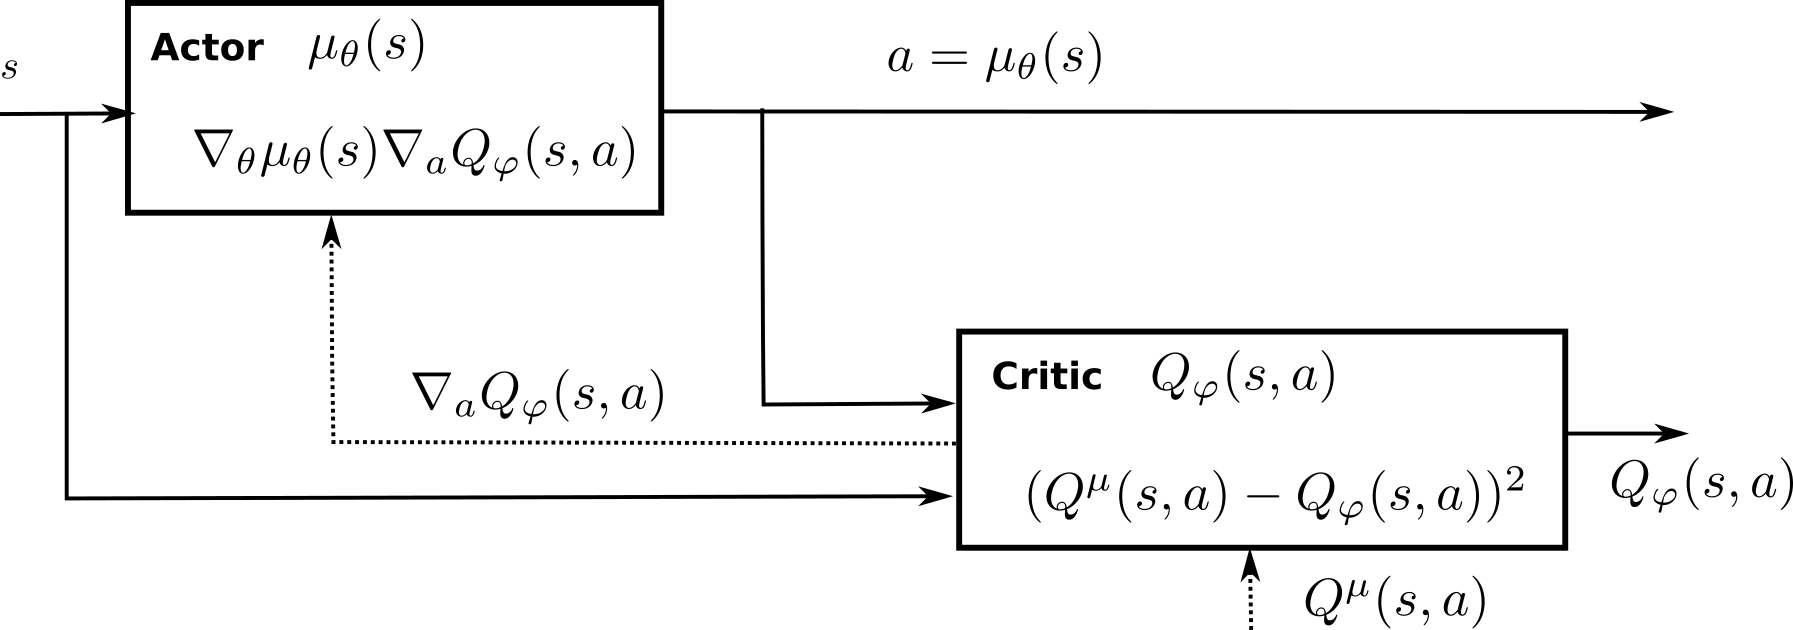
\includegraphics[width=0.95\textwidth,height=\textheight]{./img/dpg.png}

}

\caption{\label{fig-dpg}Architecture of the DPG (deterministic policy
gradient) method.}

\end{figure}

Silver et al. (2014) investigated the performance of DPG using linear
function approximators and showed that it compared positively to
stochastic algorithms in high-dimensional or continuous action spaces.
However, non-linear function approximators such as deep NN would not
work yet.

\hypertarget{deep-deterministic-policy-gradient-ddpg}{%
\subsection{Deep Deterministic Policy Gradient
(DDPG)}\label{deep-deterministic-policy-gradient-ddpg}}

Lillicrap et al. (2015) extended the DPG approach to work with
non-linear function approximators. In fact, they combined ideas from DQN
and DPG to create a very successful algorithm able to solve continuous
problems off-policy, the \textbf{deep deterministic policy gradient}
(DDPG) algorithm..

The key ideas borrowed from DQN are:

\begin{itemize}
\tightlist
\item
  Using an \textbf{experience replay memory} to store past transitions
  and learn off-policy.
\item
  Using \textbf{target networks} to stabilize learning.
\end{itemize}

They modified the update frequency of the target networks originally
used in DQN. In DQN, the target networks are updated with the parameters
of the trained networks every couple of thousands of steps. The target
networks therefore change a lot between two updates, but not very often.
Lillicrap et al. (2015) found that it is actually better to make the
target networks slowly track the trained networks, by updating their
parameters after each update of the trained network using a sliding
average for both the actor and the critic:

\[
    \theta' = \tau \, \theta + (1-\tau) \, \theta'
\]

with \(\tau <<1\). Using this update rule, the target networks are
always ``late'' with respect to the trained networks, providing more
stability to the learning of Q-values.

The key idea borrowed from DPG is the policy gradient for the actor. The
critic is learned using regular Q-learning and target networks:

\[
    J(\varphi) = \mathbb{E}_{s \sim \rho_\mu}[(r(s, a, s') + \gamma \, Q_{\varphi'}(s', \mu_{\theta'}(s')) - Q_\varphi(s, a))^2]
\]

One remaining issue is \textbf{exploration}: as the policy is
deterministic, it can very quickly produce always the same actions,
missing perhaps more rewarding options. Some environments are naturally
noisy, enforcing exploration by itself, but this cannot be assumed in
the general case. The solution retained in DDPG is an \textbf{additive
noise} added to the deterministic action to explore the environment:

\[
    a_t = \mu_\theta(s_t) + \xi
\]

This additive noise could be anything, but the most practical choice is
to use an \textbf{Ornstein-Uhlenbeck} process (Uhlenbeck and Ornstein,
1930) to generate temporally correlated noise with zero mean.
Ornstein-Uhlenbeck processes are used in physics to model the velocity
of Brownian particles with friction. It updates a variable \(x_t\) using
a stochastic differential equation (SDE):

\[ dx_t = \theta (\mu - x_t) dt + \sigma dW_t \qquad \text{with} \qquad dW_t = \mathcal{N}(0, dt)\]

\(\mu\) is the mean of the process (usually 0), \(\theta\) is the
friction (how fast it varies with noise) and \(\sigma\) controls the
amount of noise. Figure~\ref{fig-OU} shows three independent runs of a
Ornstein-Uhlenbeck process: successive values of the variable \(x_t\)
vary randomly but coherently over time.

\begin{figure}

{\centering 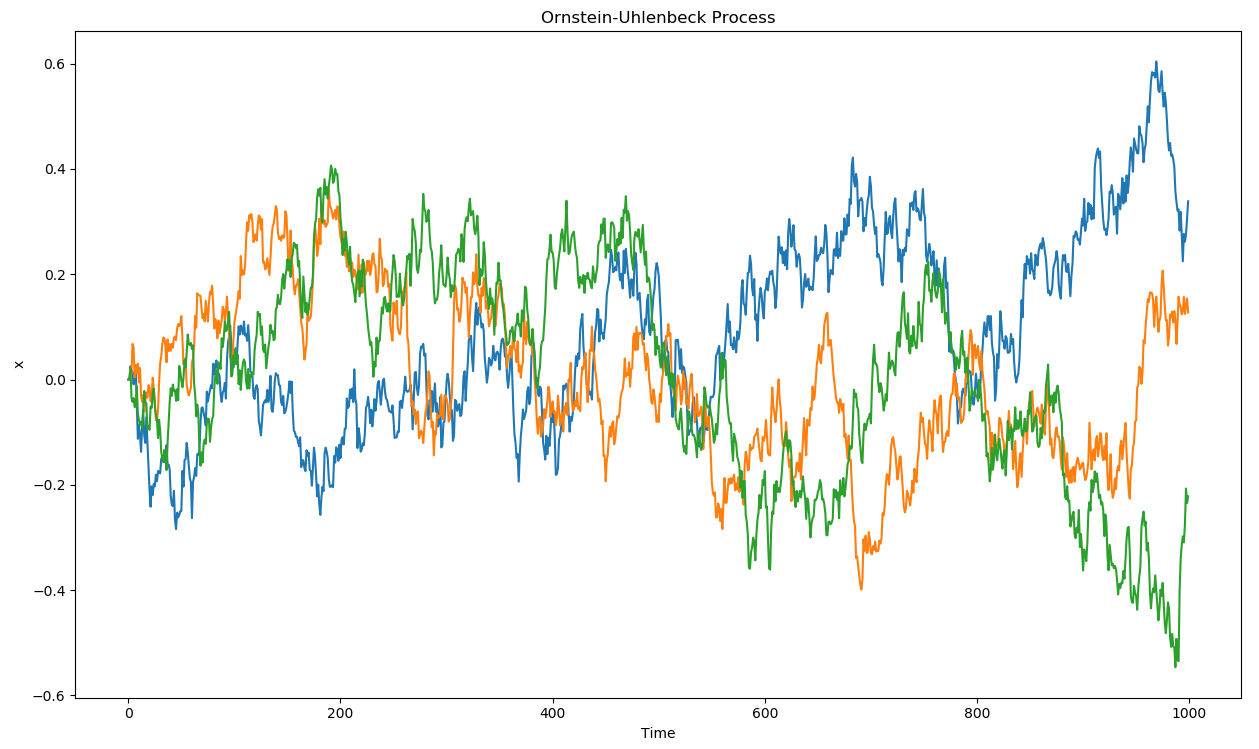
\includegraphics[width=0.8\textwidth,height=\textheight]{./img/OU.png}

}

\caption{\label{fig-OU}Three independent runs of an Ornstein-Uhlenbeck
process with \(\mu=0\), \(\sigma=0.3\), \(\theta=0.15\) and \(dt=0.1\).
The code is adapted from
\url{https://gist.github.com/jimfleming/9a62b2f7ed047ff78e95b5398e955b9e}}

\end{figure}

The architecture of the DDPG algorithm is depicted on
Figure~\ref{fig-ddpg}.

\begin{figure}

{\centering 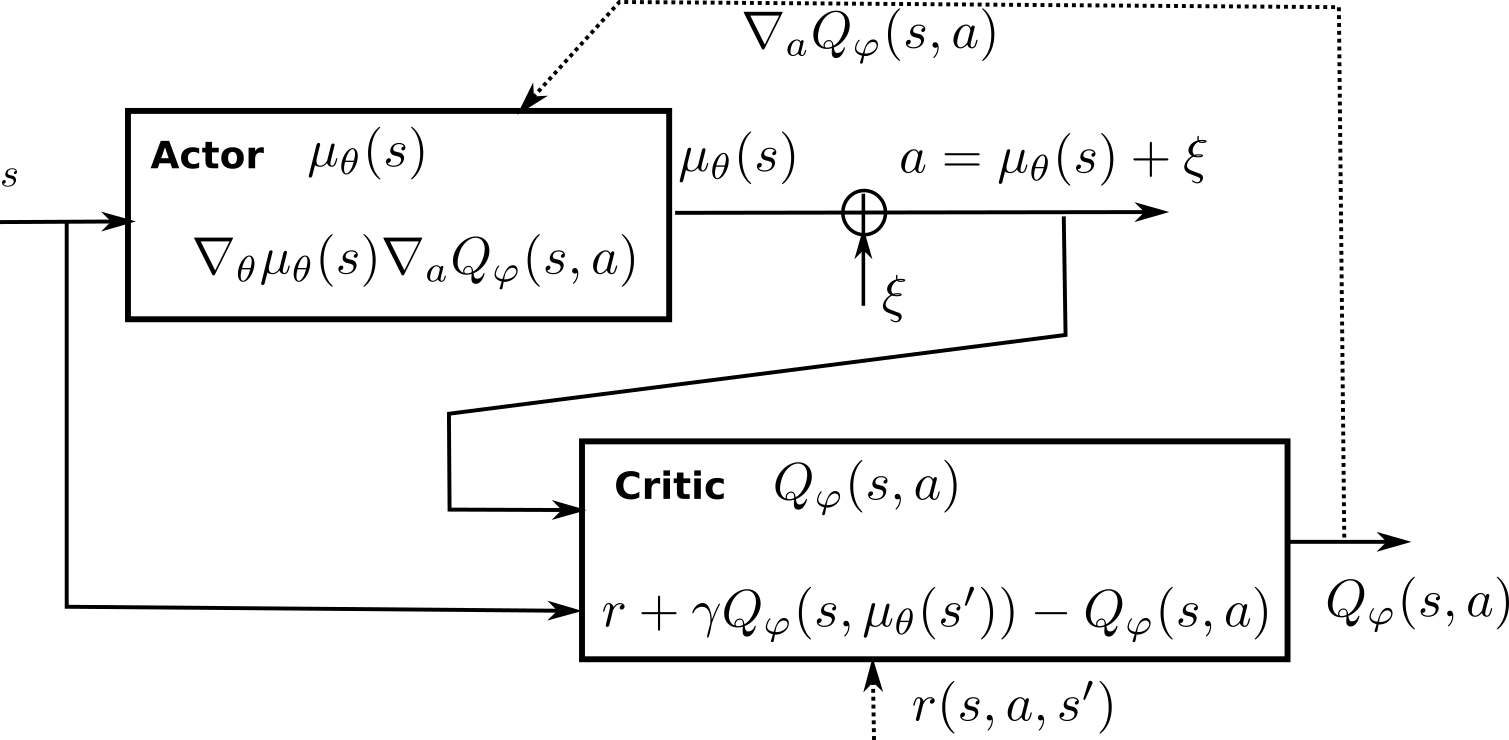
\includegraphics[width=0.7\textwidth,height=\textheight]{./img/ddpg.png}

}

\caption{\label{fig-ddpg}Architecture of the DDPG (deep deterministic
policy gradient) algorithm.}

\end{figure}

The pseudo-algorithm is as follows:

\begin{center}\rule{0.5\linewidth}{0.5pt}\end{center}

\begin{itemize}
\item
  Initialize actor network \(\mu_{\theta}\) and critic \(Q_\varphi\)
  with random weights.
\item
  Create the target networks \(\mu_{\theta'}\) and \(Q_{\varphi'}\).
\item
  Initialize experience replay memory \(\mathcal{D}\) of maximal size
  \(N\).
\item
  for episode \(\in [1, M]\):

  \begin{itemize}
  \tightlist
  \item
    Initialize random process \(\xi\).
  \item
    Observe the initial state \(s_0\).
  \item
    for \(t \in [0, T_\text{max}]\):

    \begin{itemize}
    \item
      Select the action \(a_t = \mu_\theta(s_t) + \xi\) according to the
      current policy and the noise.
    \item
      Perform the action \(a_t\) and observe the next state \(s_{t+1}\)
      and the reward \(r_{t+1}\).
    \item
      Store \((s_t, a_t, r_{t+1}, s_{t+1})\) in the experience replay
      memory.
    \item
      Sample a minibatch of \(N\) transitions randomly from
      \(\mathcal{D}\).
    \item
      For each transition \((s_k, a_k, r_k, s'_k)\) in the minibatch:

      \begin{itemize}
      \tightlist
      \item
        Compute the target value using target networks
        \(y_k = r_k + \gamma \, Q_{\varphi'}(s'_k, \mu_{\theta'}(s'_k))\).
      \end{itemize}
    \item
      Update the critic by minimizing: \[
        \mathcal{L}(\varphi) = \frac{1}{N} \sum_k (y_k - Q_\varphi(s_k, a_k))^2
        \]
    \item
      Update the actor using the sampled policy gradient: \[
        \nabla_\theta J(\theta) = \frac{1}{N} \sum_k \nabla_\theta \mu_\theta(s_k) \times \nabla_a Q_\varphi(s_k, a) |_{a = \mu_\theta(s_k)}
        \]
    \item
      Update the target networks:
      \[\theta' \leftarrow \tau \theta + (1-\tau) \, \theta'\]
      \[\varphi' \leftarrow \tau \varphi + (1-\tau) \, \varphi'\]
    \end{itemize}
  \end{itemize}
\end{itemize}

\begin{center}\rule{0.5\linewidth}{0.5pt}\end{center}

The question that arises is how to obtain the gradient of the Q-value
w.r.t the action \(\nabla_a Q_\varphi(s, a)\), when the critic only
outputs the Q-value \(Q_\varphi(s, a)\). Fortunately, deep neural
networks are simulated using automatic differentiation libraries such as
tensorflow, theano, pytorch and co, which can automatically output this
gradient. If not available, one could simply use the finite difference
method (Euler) to approximate this gradient. One has to evaluate the
Q-value in \(a +da\), where \(da\) is a very small change of the
executed action, and estimate the gradient using:

\[
    \nabla_a Q_\varphi(s, a) \approx \frac{Q_\varphi(s, a + da) - Q_\varphi(s, a)}{da}
\]

Note that the DDPG algorithm is \textbf{off-policy}: the samples used to
train the actor come from the replay buffer, i.e.~were generated by an
older version of the target policy. DDPG does not rely on importance
sampling: as the policy is deterministic (we maximize
\(\mathbb{E}_{s}[Q(s, \mu_\theta(s))]\)), there is no need to balance
the probabilities of the behavior and target policies (with stochastic
policies, one should maximize
\(\mathbb{E}_{s}[\sum_{a\in\mathcal{A}} \pi(s, a) Q(s, a)]\)). In other
words, the importance sampling weight can safely be set to 1 for
deterministic policies.

DDPG has rapidly become the state-of-the-art model-free method for
continuous action spaces (although now PPO is preferred). It is able to
learn efficent policies on most contiuous problems, either pixel-based
or using individual state variables. In the original DDPG paper, they
showed that \emph{batch normalization} (Ioffe and Szegedy, 2015) is
crucial in stabilizing the training of deep networks on such problems.
Its main limitation is its high sample complexity. Distributed versions
of DDPG have been proposed to speed up learning, similarly to the
parallel actor learners of A3C (Barth-Maron et al., 2018; Lötzsch et
al., 2017; Popov et al., 2017).

\textbf{Additional references:} see
\url{http://pemami4911.github.io/blog/2016/08/21/ddpg-rl.html} for
additional explanations and step-by-step tensorflow code and
\url{https://lilianweng.github.io/lil-log/2018/04/08/policy-gradient-algorithms.html}
for contextual explanations.

\hypertarget{distributed-distributional-ddpg-d4pg}{%
\subsection{Distributed Distributional DDPG
(D4PG)}\label{distributed-distributional-ddpg-d4pg}}

Similarly to the Rainbow DQN for DQN. Distributed Distributional DDPG
(D4PG, Barth-Maron et al., 2018) proposed several improvements on DDPG
to make it more efficient:

\begin{enumerate}
\def\labelenumi{\arabic{enumi}.}
\item
  The critic is trained using \textbf{distributional learning}
  (Bellemare et al. (2017)) instead of classical Q-learning to improve
  the stability of learning in the actor (less variance).
\item
  The critic uses \textbf{n-step} returns instead of simple one-step TD
  returns as in A3C (Mnih et al. (2016)).
\item
  \textbf{Multiple Distributed Parallel Actors} gather \((s, a, r, s')\)
  transitions in parallel and write them to the same replay buffer (as
  in distributed DQN).
\item
  The replay buffer uses \textbf{Prioritized Experience Replay} (Schaul
  et al., 2015) to sample transitions based the information gain.
\end{enumerate}

\bookmarksetup{startatroot}

\hypertarget{natural-gradients}{%
\chapter{Natural Gradients}\label{natural-gradients}}

The deep networks used as function approximators in the methods
presented until now were all optimized (trained) using
\textbf{stochastic gradient descent} (SGD) or any of its variants
(RMSProp, Adam, etc). The basic idea is to change the parameters
\(\theta\) in the opposite direction of the gradient of the loss
function (or the same direction as the policy gradient, in which case it
is called gradient ascent), proportionally to a small learning rate
\(\eta\):

\[
    \Delta \theta = - \eta \, \nabla_\theta \mathcal{L}(\theta)
\]

SGD is also called a \textbf{steepest descent method}: one searches for
the smallest parameter change \(\Delta \theta\) inducing the biggest
negative change of the loss function. In classical supervised learning,
this is what we want: we want to minimize the loss function as fast as
possible, while keeping weight changes as small as possible, otherwise
learning might become unstable (weight changes computed for a single
minibatch might erase the changes made on previous minibatches). The
main difficulty of supervised learning is to choose the right value for
the learning rate: too high and learning is unstable; too low and
learning takes forever.

In deep RL, we have an additional problem: the problem is not
stationary. In Q-learning, the target
\(r(s, a, s') + \gamma \, \max_{a'} Q_\theta(S', a')\) is changing with
\(\theta\). If the Q-values change a lot between two minibatches, the
network will not get any stable target signal to learn from, and the
policy will end up suboptimal. The trick is to use \textbf{target
networks} to compute the target, which can be either an old copy of the
current network (vanilla DQN), or a smoothed version of it (DDPG).
Obviously, this introduces a bias (the targets are always wrong during
training), but this bias converges to zero (after sufficient training,
the targets will be almost correct), at the cost of a huge sample
complexity.

Target networks cannot be used in \textbf{on-policy} methods, especially
actor-critic architectures.The critic must learn from transitions
recently generated by the actor (although importance sampling and the
Retrace algorithm might help). The problem with on-policy methods is
that they waste a lot of data: they always need fresh samples to learn
from and never reuse past experiences. The policy gradient theorem shows
why:

\[
\begin{aligned}
    \nabla_\theta J(\theta) & =  \mathbb{E}_{s \sim \rho_\theta, a \sim \pi_\theta}[\nabla_\theta \log \pi_\theta(s, a) \, Q^{\pi_\theta}(s, a)] \\
    & \approx  \mathbb{E}_{s \sim \rho_\theta, a \sim \pi_\theta}[\nabla_\theta \log \pi_\theta(s, a) \, Q_\varphi(s, a)]
\end{aligned}
\]

If the policy \(\pi_\theta\) changes a lot between two updates, the
estimated Q-value \(Q_\varphi(s, a)\) will represent the value of the
action for a totally different policy, not the true Q-value
\(Q^{\pi_\theta}(s, a)\). The estimated policy gradient will then be
strongly biased and learning will be suboptimal. In other words, the
actor should not change much faster than the critic, and vice versa. A
naive solution would be to use a very small learning rate for the actor,
but this just slows down learning (adding to the sample complexity)
without solving the problem.

To solve the problem, we should actually do the opposite of the steepest
descent: \emph{search for the biggest parameter change \(\Delta \theta\)
inducing the smallest change in the policy, but in the right direction}.
If the parameter change is high, the actor will learn a lot internally
from each experience. But if the policy change is small between two
updates (although the parameters have changed a lot), we might be able
to reuse past experiences, as the targets will not be that wrong.

This is where \textbf{natural gradients} come into play, which are
originally a statistical method to optimize over spaces of probability
distributions, for example for variational inference. The idea to use
natural gradients to train neural networks comes from Amari (1998).
Kakade (2001) applied natural gradients to policy gradient methods,
while Peters and Schaal (2008) proposed a natural actor-critic algorithm
for linear function approximators. The idea was adapted to deep RL by
Schulman and colleagues, with Trust Region Policy Optimization (TRPO,
Schulman et al., 2015b) and Proximal Policy Optimization (PPO, Schulman
et al., 2017a), the latter gaining momentum over DDPG as the go-to
method for continuous RL problems, particularly because of its smaller
sample complexity and its robustness to hyperparameters.

\hypertarget{principle-of-natural-gradients}{%
\subsection{Principle of natural
gradients}\label{principle-of-natural-gradients}}

\begin{figure}

{\centering 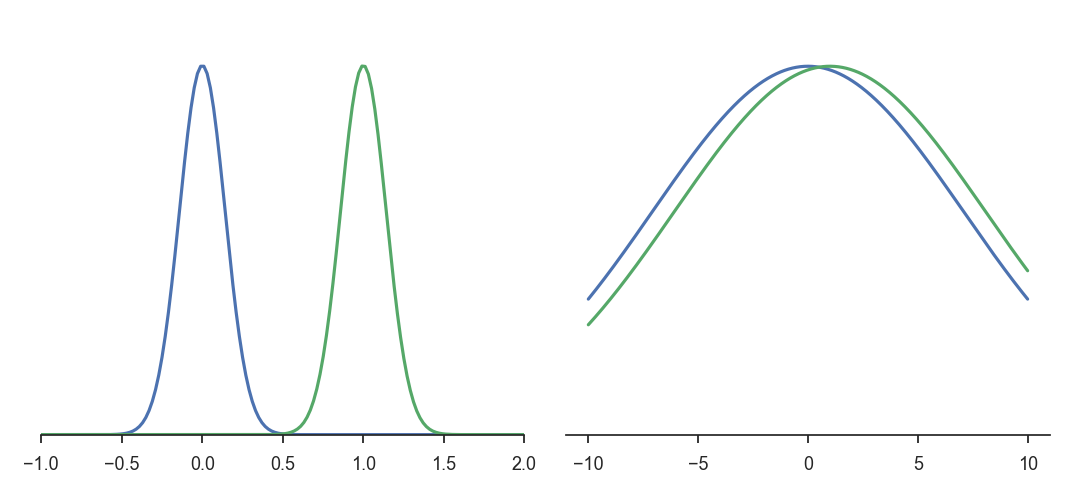
\includegraphics[width=0.8\textwidth,height=\textheight]{./img/naturalgradient.png}

}

\caption{\label{fig-naturalgradient}Euclidian distances in the parameter
space do not represent well the statistical distance between probability
distributions. The two Gaussians on the left (\(\mathcal{N}(0, 0.2)\)
and \(\mathcal{N}(1, 0.2)\)) have the same Euclidian distance in the
parameter space
(\(d = \sqrt{(\mu_0 - \mu_1)^2+(\sigma_0 - \sigma_1)^2}\)) than the two
Gaussians on the right (\(\mathcal{N}(0, 10)\) and
\(\mathcal{N}(1, 10)\)). However, the Gaussians on the right are much
more similar than the two on the left: if you have a single sample, you
could not say from which distribution it comes for the Gaussians on the
right, while it is obvious for the Gaussians on the left.}

\end{figure}

Consider the two Gaussian distributions in the left part of
Figure~\ref{fig-naturalgradient} (\(\mathcal{N}(0, 0.2)\) and
\(\mathcal{N}(1, 0.2)\)) and the two on the right
(\(\mathcal{N}(0, 10)\) and \(\mathcal{N}(1, 10)\)). In both cases, the
distance in the Euclidian space of parameters
\(d = \sqrt{(\mu_0 - \mu_1)^2+(\sigma_0 - \sigma_1)^2}\) is the same
between the two Gaussians. Obviously, the two distributions on the left
are however further away from each other than the two on the the right.
This indicates that the Euclidian distance in the parameter space (which
is what \emph{regular} gradients act on) is not a correct measurement of
the statistical distance between two distributions (which what we want
to minimize between two iterations of PG).

In statistics, a common measurement of the statistical distance between
two distributions \(p\) and \(q\) is the \textbf{Kullback-Leibler (KL)
divergence} \(D_{KL}(p||q)\), also called relative entropy or
information gain. It is defined as:

\[
    D_{KL}(p || q) = \mathbb{E}_{x \sim p} [\log \frac{p(x)}{q(x)}]  = \int p(x) \, \log \frac{p(x)}{q(x)} \, dx
\]

Its minimum is 0 when \(p=q\) (as \(\log \frac{p(x)}{q(x)}\) is then 0)
and is positive otherwise. Minimizing the KL divergence is equivalent to
``matching'' two distributions. Note that supervised methods in machine
learning can all be interpreted as a minimization of the KL divergence:
if \(p(x)\) represents the distribution of the data (the label of a
sample \(x\)) and \(q(x)\) the one of the model (the prediction of a
neural network for the same sample \(x\)), supervised methods want the
output distribution of the model to match the distribution of the data,
i.e.~make predictions that are the same as the labels. For generative
models, this is for example at the core of \emph{generative adversarial
networks} (Arjovsky et al., 2017; Goodfellow et al., 2014) or
\emph{variational autoencoders} (Kingma and Welling, 2013).

The KL divergence is however not symmetrical
(\(D_{KL}(p || q) \neq D_{KL}(q || p)\)), so a more useful divergence is
the symmetric KL divergence, also known as Jensen-Shannon (JS)
divergence:

\[
    D_{JS}(p || q) = \frac{D_{KL}(p || q) + D_{KL}(q || p)}{2}
\]

Other forms of divergence measurements exist, such as the Wasserstein
distance which improves generative adversarial networks (Arjovsky et
al., 2017), but they are not relevant here. See
\url{https://www.alexirpan.com/2017/02/22/wasserstein-gan.html} for more
explanations.

We now have a global measurement of the similarity between two
distributions on the whole input space, but which is hard to compute.
How can we use it anyway in our optimization problem? As mentioned
above, we search for the biggest parameter change \(\Delta \theta\)
inducing the smallest change in the policy. We need a metric linking
changes in the parameters of the distribution (the weights of the
network) to changes in the distribution itself. In other terms, we will
apply gradient descent on the statistical manifold defined by the
parameters rather than on the parameters themselves.

\begin{figure}

{\centering 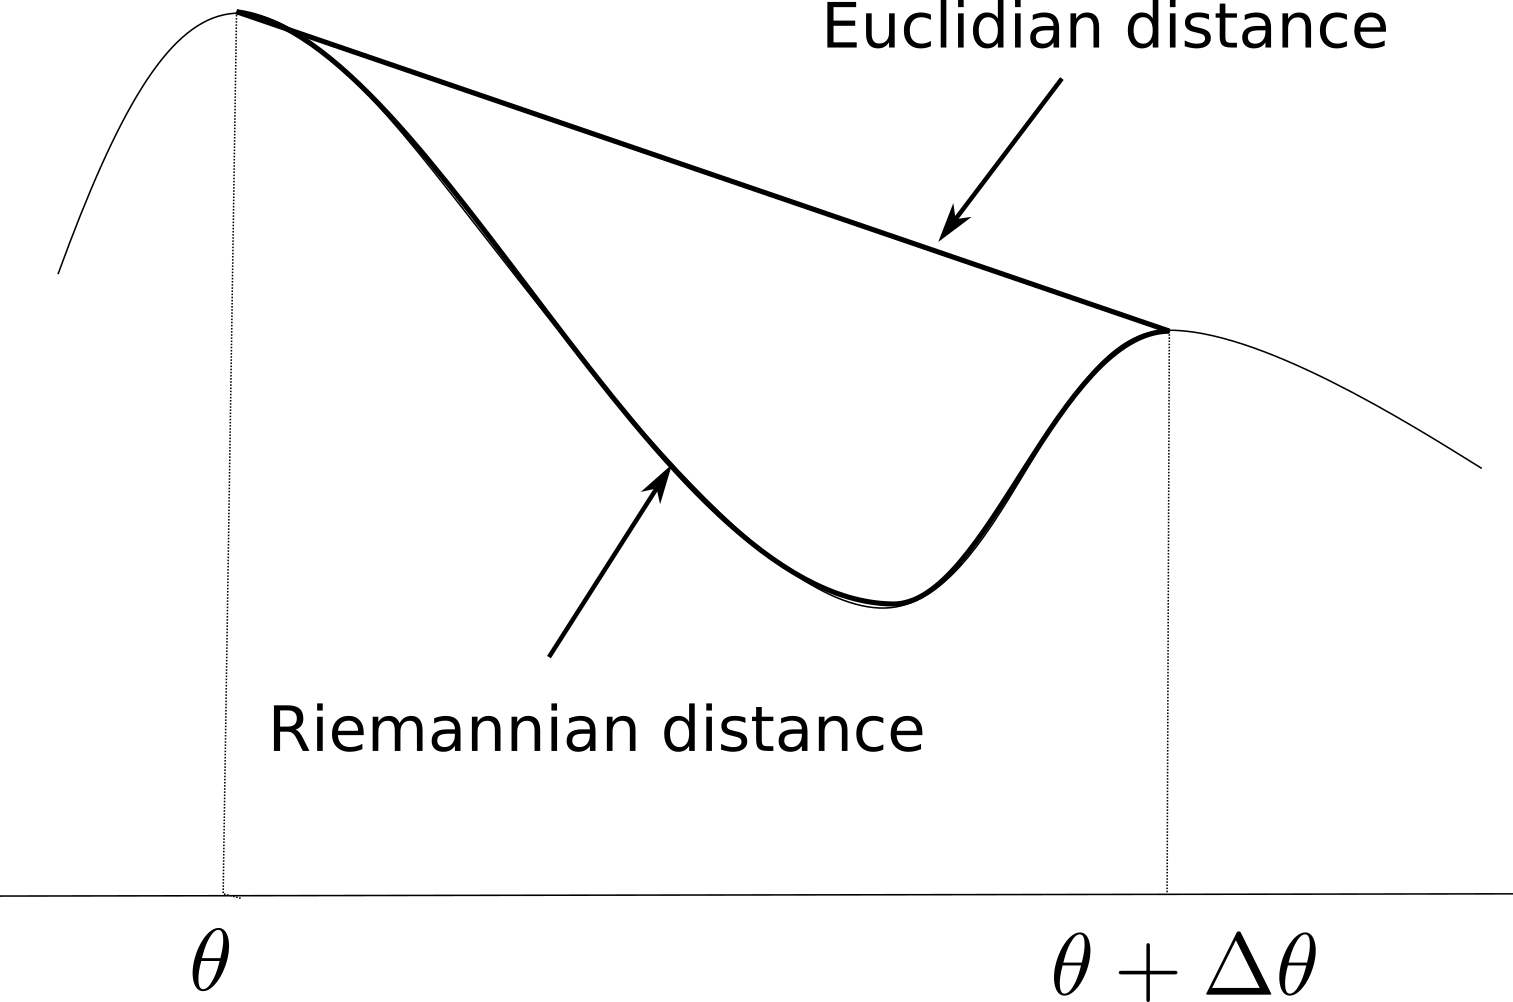
\includegraphics[width=0.5\textwidth,height=\textheight]{./img/riemannian.png}

}

\caption{\label{fig-riemannian}Naive illustration of the Riemannian
metric. The Euclidian distance between \(p(x; \theta)\) and
\(p(x; \theta + \Delta \theta)\) depends on the Euclidian distance
between \(\theta\) and \(\theta + \Delta\theta\),
i.e.~\(\Delta \theta\). Riemannian metrics follow the geometry of the
manifold to compute that distance, depending on its curvature. This
figure is only for illustration: Riemannian metrics are purely local,
\(\Delta \theta\) should be much smaller.}

\end{figure}

Let's consider a parameterized distribution \(p(x; \theta)\) and its new
value \(p(x; \theta + \Delta \theta)\) after applying a small parameter
change \(\Delta \theta\). As depicted on Figure~\ref{fig-riemannian},
the Euclidian metric in the parameter space
(\(||\theta + \Delta \theta - \theta||^2\)) does not take the structure
of the statistical manifold into account. We need to define a
\textbf{Riemannian metric} which accounts locally for the curvature of
the manifold between \(\theta\) and \(\theta + \Delta \theta\). The
Riemannian distance is defined by the dot product:

\[
    ||\Delta \theta||^2 = < \Delta \theta , F(\theta) \, \Delta \theta >
\]

where \(F(\theta)\) is called the Riemannian metric tensor and is an
inner product on the tangent space of the manifold at the point
\(\theta\).

When using the symmetric KL divergence to measure the distance between
two distributions, the corresponding Riemannian metric is the
\textbf{Fisher Information Matrix} (FIM), defined as the Hessian matrix
of the KL divergence around \(\theta\), i.e.~the matrix of second order
derivatives w.r.t the elements of \(\theta\). See
\url{https://stats.stackexchange.com/questions/51185/connection-between-fisher-metric-and-the-relative-entropy}
and
\url{https://wiseodd.github.io/techblog/2018/03/14/natural-gradient/}
for an explanation of the link between the Fisher matrix and KL
divergence.

The Fisher information matrix is defined as the Hessian of the KL
divergence around \(\theta\), i.e.~how the manifold locally changes
around \(\theta\):

\[
    F(\theta) = \nabla^2 D_{JS}(p(x; \theta) || p(x; \theta + \Delta \theta))|_{\Delta \theta = 0}
\]

which necessitates to compute second order derivatives which are very
complex and slow to obtain, especially when there are many parameters
\(\theta\) (the weights of the NN). Fortunately, it also has a simpler
form which only depends on the outer product between the gradients of
the log-likelihoods:

\[
    F(\theta) = \mathbb{E}_{x \sim p(x, \theta)}[ \nabla \log p(x; \theta)  (\nabla \log p(x; \theta))^T]
\]

which is something we can easily sample and compute.

Why is it useful? The Fisher Information matrix allows to
\textbf{locally} approximate (for small \(\Delta \theta\)) the KL
divergence between the two close distributions (using a second-order
Taylor series expansion):

\[
    D_{JS}(p(x; \theta) || p(x; \theta + \Delta \theta)) \approx \Delta \theta^T \, F(\theta) \, \Delta \theta
\]

The KL divergence is then locally quadratic, which means that the update
rules obtained when minimizing the KL divergence with gradient descent
will be linear. Suppose we want to minimize a loss function \(L\)
parameterized by \(\theta\) and depending on the distribution \(p\).
\textbf{Natural gradient descent} (Amari, 1998) attempts to move along
the statistical manifold defined by \(p\) by correcting the gradient of
\(L(\theta)\) using the local curvature of the KL-divergence surface,
i.e.~moving some given distance in the direction
\(\tilde{\nabla_\theta} L(\theta)\):

\[
    \tilde{\nabla_\theta} L(\theta) = F(\theta)^{-1} \, \nabla_\theta L(\theta)
\]

\(\tilde{\nabla_\theta} L(\theta)\) is the \textbf{natural gradient} of
\(L(\theta)\). Natural gradient descent simply takes steps in this
direction:

\[
    \Delta \theta = - \eta \, \tilde{\nabla_\theta} L(\theta)
\]

When the manifold is not curved (\(F(\theta)\) is the identity matrix),
natural gradient descent is the regular gradient descent.

But what is the advantage of natural gradients? The problem with regular
gradient descent is that it relies on a fixed learning rate. In regions
where the loss function is flat (a plateau), the gradient will be almost
zero, leading to very slow improvements. Because the natural gradient
depends on the inverse of the curvature (Fisher), the magnitude of the
gradient will be higher in flat regions, leading to bigger steps, and
smaller in very steep regions (around minima). Natural GD therefore
converges faster and better than regular GD.

Natural gradient descent is a generic optimization method, it can for
example be used to train more efficiently deep networks in supervised
learning. Its main drawback is the necessity to inverse the Fisher
information matrix, whose size depends on the number of free parameters
(if you have N weights in the NN, you need to inverse a NxN matrix).
Several approximations allows to remediate to this problem, for example
Conjugate Gradients or Kronecker-Factored Approximate Curvature (K-FAC).

\textbf{Additional resources} to understand natural gradients:

\begin{itemize}
\tightlist
\item
  \url{http://andymiller.github.io/2016/10/02/natural_gradient_bbvi.html}
\item
  \url{https://hips.seas.harvard.edu/blog/2013/01/25/the-natural-gradient/}
\item
  \url{http://kvfrans.com/what-is-the-natural-gradient-and-where-does-it-appear-in-trust-region-policy-optimization}
\item
  \url{https://wiseodd.github.io/techblog/2018/03/14/natural-gradient/}
\item
  A tutorial by John Schulman (OpenAI)
  \url{https://www.youtube.com/watch?v=xvRrgxcpaHY}
\item
  A blog post on the related Hessian-free optimization and conjuguate
  gradients
  \url{http://andrew.gibiansky.com/blog/machine-learning/hessian-free-optimization/}
\item
  K-FAC:
  \url{https://syncedreview.com/2017/03/25/optimizing-neural-networks-using-structured-probabilistic-models/}
\item
  Conjugate gradients:
  \url{https://www.cs.cmu.edu/~quake-papers/painless-conjugate-gradient.pdf}
\end{itemize}

\textbf{Note:} Natural gradients can also be used to train DQN
architectures, resulting in more efficient and stable learning behaviors
(Knight and Lerner, 2018).

\hypertarget{natural-policy-gradient-and-natural-actor-critic-nac}{%
\subsection{Natural policy gradient and Natural Actor Critic
(NAC)}\label{natural-policy-gradient-and-natural-actor-critic-nac}}

Kakade (2001) applied the principle of natural gradients proposed by
Amari (1998) to the policy gradient theorem:

\[
    \nabla_\theta J(\theta) =  \mathbb{E}_{s \sim \rho_\theta, a \sim \pi_\theta}[\nabla_\theta \log \pi_\theta(s, a) \, Q^{\pi_\theta}(s, a)]
\]

This \emph{regular} gradient does not take into account the underlying
structure of the policy distribution \(\pi(s, a)\). The Fisher
information matrix for the policy is defined by:

\[
    F(\theta) = \mathbb{E}_{s \sim \rho_\theta, a \sim \pi_\theta}[ \nabla \log \pi_\theta(s, a)  (\nabla \log \pi_\theta(s, a))^T]
\]

The natural policy gradient is simply:

\[
    \tilde{\nabla}_\theta J(\theta) = F(\theta)^{-1} \, \nabla_\theta J(\theta)  = \mathbb{E}_{s \sim \rho_\theta, a \sim \pi_\theta}[ F(\theta)^{-1} \,  \nabla_\theta \log \pi_\theta(s, a) \, Q^{\pi_\theta}(s, a)]
\]

Kakade (2001) also shows that you can replace the true Q-value
\(Q^{\pi_\theta}(s, a)\) with a compatible approximation
\(Q_\varphi(s, a)\) (as long as it minimizes the quadratic error) and
still obtained an unbiased natural gradient. An important theoretical
result is that policy improvement is guaranteed with natural gradients:
the new policy after an update is always better (more expected returns)
than before. He experimented this new rule on various simple MDPs and
observed drastic improvements over vanilla PG.

Peters and Schaal (2008) extended on the work of Kakade (2001) to
propose the natural actor-critic (NAC). The exact derivations would be
too complex to summarize here, but the article is an interesting read.
He particularly reviews the progress at that time on policy gradient for
its use in robotics. He showed that the \(F(\theta)\)) is a true Fisher
information matrix even when using sampled episodes, and derived a
baseline \(b\) to reduce the variance of the natural policy gradient. He
demonstrated the power of this algorithm by letting a robot learning
motor primitives for baseball.

\hypertarget{trust-region-policy-optimization-trpo}{%
\subsection{Trust Region Policy Optimization
(TRPO)}\label{trust-region-policy-optimization-trpo}}

\hypertarget{principle}{%
\subsubsection*{Principle}\label{principle}}
\addcontentsline{toc}{subsubsection}{Principle}

Schulman et al. (2015b) extended the idea of natural gradients to allow
their use for non-linear function approximators (e.g.~deep networks), as
the previous algorithms only worked efficiently for linear
approximators. The proposed algorithm, Trust Region Policy Optimization
(TRPO), has now been replaced in practice by Proximal Policy
Optimization (PPO, see next section) but its novel ideas are important
to understand already.

Let's note the expected return of a policy \(\pi\) as:

\[
    \eta(\pi) = \mathbb{E}_{s \sim \rho_\pi, a \sim \pi}[\sum_{t=0}^\infty \gamma^t \, r(s_t, a_t, s_{t+1})]
\]

where \(\rho_\pi\) is the discounted visitation frequency distribution
(the probability that a state \(s\) will be visited at some point in
time by the policy \(\pi\)):

\[
    \rho_\pi(s) = P(s_0=s) + \gamma \, P(s_1=s) + \gamma^2 \, P(s_2=s) + \ldots
\]

Kakade and Langford (2002) had shown that it is possible to relate the
expected return of two policies \(\pi_\theta\) and
\(\pi_{\theta_\text{old}}\) using advantages (omitting \(\pi\) in the
notations):

\[
    \eta(\theta) = \eta(\theta_\text{old}) + \mathbb{E}_{s \sim \rho_{\pi_\theta}, a \sim \pi_\theta} [A_{\pi_{\theta_\text{old}}}(s, a)]
\]

The advantage \(A_{\pi_{\theta_\text{old}}}(s, a)\) denotes the change
in the expected return obtained after \((s, a)\) when using the new
policy \(\pi_\theta\), in comparison to the one obtained with the old
policy \(\pi_{\theta_\text{old}}\). While this formula seems interesting
(it measures how good the new policy is with regard to the average
performance of the old policy, so we could optimize directly), it is
difficult to estimate as the mathematical expectation depends on
state-action pairs generated by the new policy :
\(s \sim \rho_{\pi_\theta}, a \sim \pi_\theta\).

Schulman et al. (2015b) propose an approximation to this formula, by
considering that if the two policies \(\pi_\theta\) and
\(\pi_{\theta_\text{old}}\) are not very different from another, one can
sample the states from the old distribution:

\[
    \eta(\theta) \approx \eta(\theta_\text{old}) + \mathbb{E}_{s \sim \rho_{\pi_{\theta_\text{old}}}, a \sim \pi_\theta} [A_{\pi_{\theta_\text{old}}}(s, a)]
\]

One can already recognize the main motivation behind natural gradients:
finding a weight update that moves the policy in the right direction
(getting more rewards) while keeping the change in the policy
distribution as small as possible (to keep the assumption correct).

Let's now define the following objective function:

\[
    J_{\theta_\text{old}}(\theta) = \eta(\theta_\text{old}) + \mathbb{E}_{s \sim \rho_{\pi_{\theta_\text{old}}}, a \sim \pi_\theta} [A_{\pi_{\theta_\text{old}}}(s, a)]
\]

It is easy to see that
\(J_{\theta_\text{old}}(\theta_\text{old}) = \eta(\theta_\text{old})\)
by definition of the advantage, and that its gradient w.r.t to
\(\theta\) taken in \(\theta_\text{old}\) is the same as the one of
\(\eta(\theta_\text{old})\):

\[
    \nabla_\theta J_{\theta_\text{old}}(\theta)|_{\theta = \theta_\text{old}} = \nabla_\theta \eta(\theta)|_{\theta = \theta_\text{old}}
\]

This means that, at least locally, one maximization step of
\(J_{\theta_\text{old}}(\theta)\) goes in the same direction as
maximizing \(\eta(\theta)\) if we do not go too far. \(J\) is called a
\textbf{surrogate objective function}: it is not what we want to
optimize, but it leads to the same result. TRPO belongs to the class of
\textbf{minorization-majorization} algorithms (MM, we first find a local
lower bound and then maximize it, iteratively).

Let's now suppose that we can find its maximum, i.e.~a policy \(\pi'\)
that maximizes the advantage of each state-action pair over
\(\pi_{\theta_\text{old}}\). There would be no guarantee that \(\pi'\)
and \(\pi_{\theta_\text{old}}\) are close enough so that the assumption
stands. We could therefore make only a small step in its direction and
hope for the best:

\begin{equation}\protect\hypertarget{eq-linesearch}{}{
    \pi_\theta(s, a) = (1-\alpha) \, \pi_{\theta_\text{old}}(s, a) + \alpha \, \pi'(s,a)
}\label{eq-linesearch}\end{equation}

This is the conservative policy iteration method of Kakade and Langford
(2002), where a bound on the difference between
\(\eta(\pi_{\theta_\text{old}})\) and \(J_{\theta_\text{old}}(\theta)\)
can be derived.

Schulman et al. (2015b) propose to penalize instead the objective
function by the KL divergence between the new and old policies. There
are basically two ways to penalize an optimization problem:

\begin{enumerate}
\def\labelenumi{\arabic{enumi}.}
\tightlist
\item
  Adding a hard constraint on the KL divergence, leading to a
  constrained optimization problem (where Lagrange methods can be
  applied):
\end{enumerate}

\[
    \text{maximize}_\theta \qquad J_{\theta_\text{old}}(\theta) \\
    \qquad \text{subject to} \qquad D_{KL}(\pi_{\theta_\text{old}} || \pi_\theta) \leq \delta
\]

\begin{enumerate}
\def\labelenumi{\arabic{enumi}.}
\setcounter{enumi}{1}
\tightlist
\item
  Regularizing the objective function with the KL divergence:
\end{enumerate}

\[
    \text{maximize}_\theta \qquad L(\theta) = J_{\theta_\text{old}}(\pi_\theta) - C \,  D_{KL}(\pi_{\theta_\text{old}} || \pi_\theta)
\]

In the first case, we force the KL divergence to stay below a certain
threshold. In the second case, we penalize solutions that would maximize
\(J_{\theta_\text{old}}(\theta)\) but would be too different from the
previous policy. In both cases, we want to find a policy \(\pi_\theta\)
maximizing the expected return (the objective), but which is still close
(in terms of KL divergence) from the current one. Both methods are
however sensible to the choice of the parameters \(\delta\) and \(C\).

Formally, the KL divergence
\(D_{KL}(\pi_{\theta_\text{old}} || \pi_\theta)\) should be the maximum
KL divergence over the state space:

\[
    D^\text{max}_{KL}(\pi_{\theta_\text{old}} || \pi_\theta) = \max_s D_{KL}(\pi_{\theta_\text{old}}(s, .) || \pi_\theta(s, .))
\]

This maximum KL divergence over the state space would be very hard to
compute. Empirical evaluations showed however that it is safe to use the
mean KL divergence, or even to sample it:

\[
    \bar{D}_{KL}(\pi_{\theta_\text{old}} || \pi_\theta) = \mathbb{E}_s [D_{KL}(\pi_{\theta_\text{old}}(s, .) || \pi_\theta(s, .))] \approx \frac{1}{N} \sum_{i=1}^N D_{KL}(\pi_{\theta_\text{old}}(s_i, .) || \pi_\theta(s_i, .))
\]

\hypertarget{trust-regions}{%
\subsubsection*{Trust regions}\label{trust-regions}}
\addcontentsline{toc}{subsubsection}{Trust regions}

\begin{figure}

{\centering 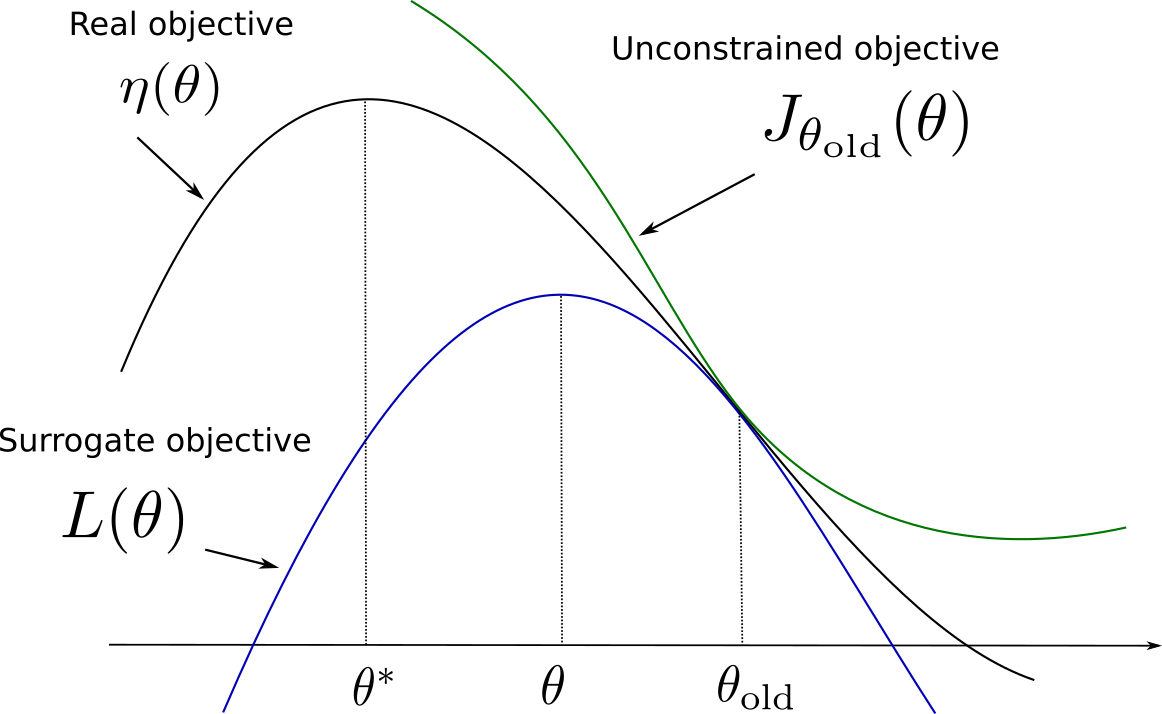
\includegraphics[width=0.7\textwidth,height=\textheight]{./img/trustregion.png}

}

\caption{\label{fig-trustregion}Graphical illustration of trust regions.
From the current parameters \(\theta_\text{old}\), we search for the
maximum \(\theta^*\) of the real objective \(\eta(\theta)\). The
unconstrained objective \(J_{\theta_\text{old}}(\theta)\) is locally
similar to \(\eta(\theta)\) but quickly diverge as \(\pi_\theta\) and
\(\pi_{\theta_\text{old}}\) become very different. The surrogate
objective
\(L(\theta) = J_{\theta_\text{old}} (\theta) - C \, D_{KL}(\pi_{\theta_\text{old}} || \pi_\theta)\)
is always smaller than \(\eta(\theta)\) and has a maximum close to
\(\theta^*\) which keeps \(\pi_\theta\) and \(\pi_{\theta_\text{old}}\)
close from each other in terms of KL divergence. The region around
\(\theta_\text{old}\) where big optimization steps can be taken without
changing the policy too much is called the trust region.}

\end{figure}

Before diving further into how these optimization problems can be
solved, let's wonder why the algorithm is called \textbf{trust region
policy optimization} using the regularized objective.
Figure~\ref{fig-trustregion} illustrates the idea. The ``real''
objective function \(\eta(\theta)\) should be maximized (with gradient
descent or similar) starting from the parameters \(\theta_\text{old}\).
We cannot estimate the objective function directly, so we build a
surrogate objective function
\(L(\theta) = J_{\theta_\text{old}} (\theta) - C \, D_{KL}(\pi_{\theta_\text{old}} || \pi_\theta)\).
We know that:

\begin{enumerate}
\def\labelenumi{\arabic{enumi}.}
\tightlist
\item
  The two objectives have the same value in \(\theta_\text{old}\):
  \[L(\theta_\text{old}) = J_{\theta_\text{old}}(\theta_\text{old}) - C \,  D_{KL}(\pi_{\theta_\text{old}} || \pi_{\theta_\text{old}}) = \eta(\theta_\text{old})\]
\item
  Their gradient w.r.t \(\theta\) are the same in \(\theta_\text{old}\):
  \[\nabla_\theta L(\theta)|_{\theta = \theta_\text{old}} = \nabla_\theta \eta(\theta)|_{\theta = \theta_\text{old}}\]
\item
  The surrogate objective is always smaller than the real objective, as
  the KL divergence is positive:
  \[\eta(\theta) \geq J_{\theta_\text{old}}(\theta) - C \,  D_{KL}(\pi_{\theta_\text{old}} || \pi_\theta)\].
\end{enumerate}

Under these conditions, the surrogate objective is also called a
\textbf{lower bound} of the primary objective. The interesting fact is
that the value of \(\theta\) that maximizes \(L(\theta)\) is at the same
time:

\begin{itemize}
\tightlist
\item
  A big step in the parameter space towards the maximum of
  \(\eta(\theta)\), as \(\theta\) and \(\theta_\text{old}\) can be very
  different.
\item
  A small step in the policy distribution space, as the KL divergence
  between the previous and the new policies is kept small.
\end{itemize}

Exactly what we needed! The parameter region around
\(\theta_\text{old}\) where the KL divergence is kept small is called
the \textbf{trust region}. This means that we can safely take big
optimization steps (e.g.~with a high learning rate or even analytically)
without risking to violate the initial assumptions.

\hypertarget{sample-based-formulation}{%
\subsubsection*{Sample-based
formulation}\label{sample-based-formulation}}
\addcontentsline{toc}{subsubsection}{Sample-based formulation}

Although the theoretical proofs in Schulman et al. (2015b) used the
regularized optimization method, the practical implementation uses the
constrained optimization problem:

\[
    \text{maximize}_\theta \qquad J_{\theta_\text{old}}(\theta) = \eta(\theta_\text{old}) + \mathbb{E}_{s \sim \rho_{\pi_{\theta_\text{old}}}, a \sim \pi_\theta} [A_{\pi_{\theta_\text{old}}}(s, a)] \\
    \qquad \text{subject to} \qquad D_{KL}(\pi_{\theta_\text{old}} || \pi_\theta) \leq \delta
\]

The first thing to notice is that \(\eta(\theta_\text{old})\) does not
depend on \(\theta\), so it is constant in the optimization problem. We
only need to maximize the advantage of the actions taken by
\(\pi_\theta\) in each state visited by \(\pi_{\theta_\text{old}}\). The
problem is that \(\pi_\theta\) is what we search, so we can not sample
actions from it. The solution is to use \textbf{importance sampling} to
allow sampling actions from \(\pi_{\theta_\text{old}}\). This is
possible as long as we correct the objective with the importance
sampling weight:

\[
    \text{maximize}_\theta \qquad \mathbb{E}_{s \sim \rho_{\pi_{\theta_\text{old}}}, a \sim \pi_{\theta_\text{old}}} [\frac{\pi_\theta(s, a)}{\pi_{\theta_\text{old}}(s, a)} \, A_{\pi_{\theta_\text{old}}}(s, a)] \\
    \qquad \text{subject to} \qquad D_{KL}(\pi_{\theta_\text{old}} || \pi_\theta) \leq \delta
\]

Now that states and actions are generated by the old policy, we can
safely sample many trajectories using \(\pi_{\theta_\text{old}}\)
(Schulman et al. (2015b) proposes two methods called single path and
Vine, but we ignore it here), compute the advantages of all state-action
pairs (using real rewards along the trajectories), form the surrogate
objective function and optimize it using second-order optimization
methods.

One last thing to notice is that the advantages
\(A_{\pi_{\theta_\text{old}}}(s, a) = Q_{\pi_{\theta_\text{old}}}(s, a) - V_{\pi_{\theta_\text{old}}}(s)\)
depend on the value of the states encountered by
\(\pi_{\theta_\text{old}}\). The state values do not depend on the
policies, they are constant for each optimization step, so they can also
be safely removed:

\[
    \text{maximize}_\theta \qquad \mathbb{E}_{s \sim \rho_{\pi_{\theta_\text{old}}}, a \sim \pi_{\theta_\text{old}}} [\frac{\pi_\theta(s, a)}{\pi_{\theta_\text{old}}(s, a)} \, Q_{\pi_{\theta_\text{old}}}(s, a)] \\
    \qquad \text{subject to} \qquad D_{KL}(\pi_{\theta_\text{old}} || \pi_\theta) \leq \delta
\]

Here we go, that's TRPO. It could seem a bit disappointing to come up
with such a simple formulation (find a policy which maximizes the
Q-value of sampled actions while being not too different from the
previous one) after so many mathematical steps, but that is also the
beauty of it: not only it works, but it is guaranteed to work. With
TRPO, each optimization step brings the policy closer from an optimum,
what is called \textbf{monotonic improvement}.

\hypertarget{practical-implementation}{%
\subsubsection*{Practical
implementation}\label{practical-implementation}}
\addcontentsline{toc}{subsubsection}{Practical implementation}

Now, how do we solve the constrained optimization problem? And what is
the link with natural gradients?

To solve constrained optimization problems, we can form a Lagrange
function with an additional parameter \(\lambda\) and search for its
maximum:

\[
    \mathcal{L}(\theta, \lambda) = J_{\theta_\text{old}}(\theta)  - \lambda \, (D_{KL}(\pi_{\theta_\text{old}} || \pi_\theta) - \delta)
\]

Notice how close the Lagrange function is from the regularized problem
used in the theory. We can form a first-order approximation of
\(J_{\theta_\text{old}}(\theta)\):

\[
    J_{\theta_\text{old}}(\theta) = \nabla_\theta J_{\theta_\text{old}}(\theta) \, (\theta- \theta_\text{old})
\]

as \(J_{\theta_\text{old}}(\theta_\text{old}) = 0\).
\(g = \nabla_\theta J_{\theta_\text{old}}(\theta)\) is the now familiar
\textbf{policy gradient} with importance sampling. Higher-order terms do
not matter, as they are going to be dominated by the KL divergence term.

We will use a second-order approximation of the KL divergence term using
the Fisher Information Matrix:

\[
    D_{KL}(\pi_{\theta_\text{old}} || \pi_\theta) = (\theta- \theta_\text{old})^T \, F(\theta_\text{old}) \,  (\theta- \theta_\text{old})
\]

We get the following Lagrangian function:

\[
    \mathcal{L}(\theta, \lambda) = \nabla_\theta J_{\theta_\text{old}}(\theta) \, (\theta- \theta_\text{old})  - \lambda \, (\theta- \theta_\text{old})^T \, F(\theta_\text{old}) \,  (\theta- \theta_\text{old})
\]

which is quadratic in \(\Delta \theta = \theta- \theta_\text{old}\). It
has therefore a unique maximum, characterized by a first-order
derivative equal to 0:

\[
    \nabla_\theta J_{\theta_\text{old}}(\theta) = \lambda \, F(\theta_\text{old}) \,  \Delta \theta
\]

or:

\[
    \Delta \theta  = \frac{1}{\lambda} \, F(\theta_\text{old})^{-1} \,  \nabla_\theta J_{\theta_\text{old}}(\theta)
\]

which is the \textbf{natural gradient descent}! The size of the step
\(\frac{1}{\lambda}\) still has to be determined, but it can also be
replaced by a fixed hyperparameter.

The main problem is now to compute and inverse the Fisher information
matrix, which is quadratic with the number of parameters \(\theta\),
i.e.~with the number of weights in the NN. Schulman et al. (2015b)
proposes to used \textbf{conjugate gradients} to iteratively approximate
the Fisher, a second-order method which will not be presented here (see
\url{https://www.cs.cmu.edu/~quake-papers/painless-conjugate-gradient.pdf}
for a detailed introduction). After the conjugate gradient optimization
step, the constraint
\(D_{KL}(\pi_{\theta_\text{old}} || \pi_\theta) \leq \delta\) is however
not ensured anymore, so a line search is made as in
Equation~\ref{eq-linesearch} until that criteria is met.

\hypertarget{summary}{%
\subsubsection*{Summary}\label{summary}}
\addcontentsline{toc}{subsubsection}{Summary}

TRPO is a policy gradient method using natural gradients to
monotonically improve the expected return associated to the policy. As a
minorization-maximization (MM) method, it uses a surrogate objective
function (a lower bound on the expected return) to iteratively change
the parameters of the policy using large steps, but without changing the
policy too much (as measured by the KL divergence). Its main advantage
over DDPG is that it is much less sensible to the choice of the learning
rate.

However, it has several limitations:

\begin{itemize}
\tightlist
\item
  It is hard to use with neural networks having multiple outputs
  (e.g.~the policy and the value function, as in actor-critic methods)
  as natural gradients are dependent on the policy distribution and its
  relationship with the parameters.
\item
  It works well when the NN has only fully-connected layers, but
  empirically performs poorly on tasks requiring convolutional layers or
  recurrent layers.
\item
  The use of conjugate gradients makes the implementation much more
  complicated and less flexible than regular SGD.
\end{itemize}

\textbf{Additional resources}

\begin{itemize}
\tightlist
\item
  \url{http://178.79.149.207/posts/trpo.html}
\item
  \url{https://towardsdatascience.com/introduction-to-various-reinforcement-learning-algorithms-part-ii-trpo-ppo-87f2c5919bb9}
\item
  \url{https://medium.com/@sanketgujar95/trust-region-policy-optimization-trpo-and-proximal-policy-optimization-ppo-e6e7075f39ed}
\item
  \url{https://www.depthfirstlearning.com/2018/TRPO}
\item
  \url{http://rll.berkeley.edu/deeprlcoursesp17/docs/lec5.pdf}
\end{itemize}

\hypertarget{proximal-policy-optimization-ppo}{%
\subsection{Proximal Policy Optimization
(PPO)}\label{proximal-policy-optimization-ppo}}

Proximal Policy Optimization (PPO) was proposed by Schulman et al.
(2017a) to overcome the problems of TRPO (complexity, inability to share
parameters or to use complex NN architectures) while increasing the
range of tasks learnable by the system (compared to DQN) and improving
the sample complexity (compared to online PG methods, which perform only
one update per step).

For that, they investigated various surrogate objectives (lower bounds)
that could be solved using first-order optimization techniques (gradient
descent). Let's rewrite the surrogate loss of TRPO in the following
manner:

\[
    L^\text{CPI}(\theta) = \mathbb{E}_{t} [\frac{\pi_\theta(s_t, a_t)}{\pi_{\theta_\text{old}}(s_t, a_t)} \, A_{\pi_{\theta_\text{old}}}(s_t, a_t)] = \mathbb{E}_{t} [\rho_t(\theta) \, A_{\pi_{\theta_\text{old}}}(s_t, a_t)]
\]

by making the dependency over time explicit and noting the importance
sampling weight \(\rho_t(\theta)\). The superscript CPI refers to
conservative policy iteration (Kakade and Langford, 2002). Without a
constraint, the maximization of \(L^\text{CPI}\) would lead to an
excessively large policy updates. The authors searched how to modify the
objective, in order to penalize changes to the policy that make
\(\rho_t(\theta)\) very different from 1, i.e.~where the KL divergence
between the new and old policies would become high. They ended up with
the following surrogate loss:

\[
    L^\text{CLIP}(\theta) = \mathbb{E}_{t} [ \min (\rho_t(\theta) \, A_{\pi_{\theta_\text{old}}}(s_t, a_t), \text{clip}(\rho_t(\theta) , 1- \epsilon, 1+\epsilon) \,  A_{\pi_{\theta_\text{old}}}(s_t, a_t)]
\]

The left part of the min operator is the surrogate objective of TRPO
\(L^\text{CPI}(\theta)\). The right part restricts the importance
sampling weight between \(1-\epsilon\) and \(1 +\epsilon\). Let's
consider two cases (depicted on Figure~\ref{fig-ppo}):

\begin{figure}

{\centering 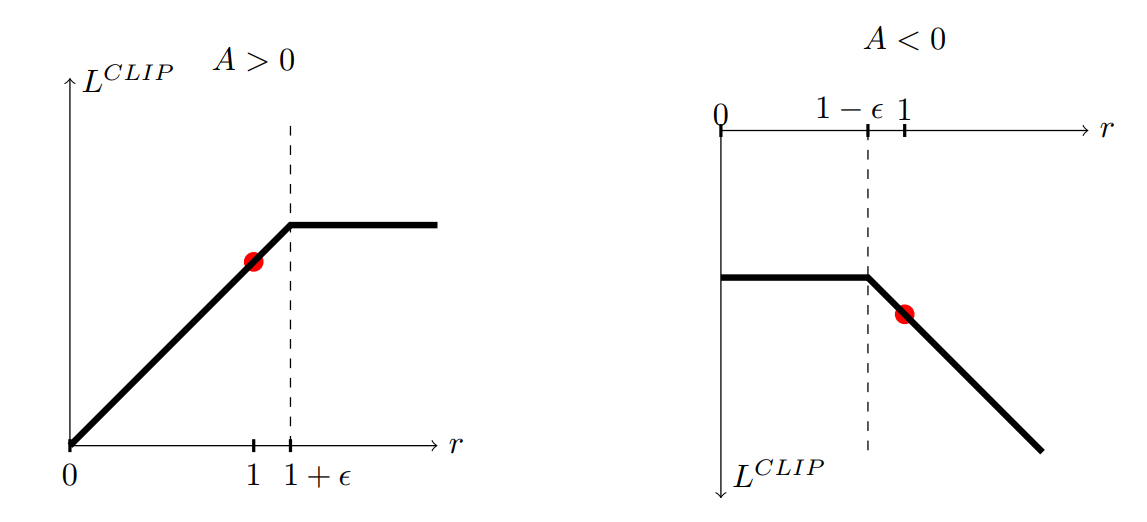
\includegraphics[width=0.8\textwidth,height=\textheight]{./img/ppo.png}

}

\caption{\label{fig-ppo}Illustration of the effect of clipping the
importance sampling weight. Taken from Schulman et al. (2017a).}

\end{figure}

\begin{enumerate}
\def\labelenumi{\arabic{enumi}.}
\item
  the transition \(s_t, a_t\) has a positive advantage, i.e.~it is a
  better action than expected. The probability of selecting that action
  again should be increased,
  i.e.~\(\pi_\theta(s_t, a_t) > \pi_{\theta_\text{old}}(s_t, a_t)\).
  However, the importance sampling weight could become very high (a
  change from 0.01 to 0.05 is a ration of \(\rho_t(\theta) = 5\)). In
  that case, \(\rho_t(\theta)\) will be clipped to \(1+\epsilon\), for
  example 1.2. As a consequence, the parameters \(\theta\) will move in
  the right direction, but the distance between the new and the old
  policies will stay small.
\item
  the transition \(s_t, a_t\) has a negative advantage, i.e.~it is a
  worse action than expected. Its probability will be decreased and the
  importance sampling weight might become much smaller than 1. Clipping
  it to \(1-\epsilon\) avoids drastic changes to the policy, while still
  going in the right direction.
\end{enumerate}

Finally, they take the minimum of the clipped and unclipped objective,
so that the final objective is a lower bound of the unclipped objective.
In the original paper, they use \textbf{generalized advantage
estimation} (GAE) to estimate \(A_{\pi_{\theta_\text{old}}}(s_t, a_t)\),
but anything could be used (n-steps, etc). Transitions are sampled by
multiple actors in parallel, as in A2C.

The pseudo-algorithm of PPO is as follows:

\begin{center}\rule{0.5\linewidth}{0.5pt}\end{center}

\begin{itemize}
\item
  Initialize an actor \(\pi_\theta\) and a critic \(V_\varphi\) with
  random weights.
\item
  while not converged :

  \begin{itemize}
  \item
    for \(N\) actors in parallel:

    \begin{itemize}
    \item
      Collect \(T\) transitions using \(\pi_\text{old}\).
    \item
      Compute the generalized advantage of each transition using the
      critic.
    \end{itemize}
  \item
    for \(K\) epochs:

    \begin{itemize}
    \item
      Sample \(M\) transitions from the ones previously collected.
    \item
      Train the actor to maximize the clipped surrogate objective.
    \item
      Train the critic to minimize the mse using TD learning.
    \end{itemize}
  \item
    \(\theta_\text{old} \leftarrow \theta\)
  \end{itemize}
\end{itemize}

\begin{center}\rule{0.5\linewidth}{0.5pt}\end{center}

The main advantage of PPO with respect to TRPO is its simplicity: the
clipped objective can be directly maximized using first-order methods
like stochastic gradient descent or Adam. It does not depend on
assumptions about the parameter space: CNNs and RNNs can be used for the
policy. It is sample-efficient, as several epochs of parameter updates
are performed between two transition samplings: the policy network
therefore needs less fresh samples that strictly on-policy algorithms to
converge.

The only drawbacks of PPO is that there no convergence guarantee
(although in practice it converges more often than other
state-of-the-art methods) and that the right value for \(\epsilon\) has
to be determined. PPO has improved the state-of-the-art on Atari games
and Mujoco robotic tasks. It has become the go-to method for continuous
control problems.

\textbf{Additional resources}

\begin{itemize}
\tightlist
\item
  More explanations and demos from OpenAI:
  \url{https://blog.openai.com/openai-baselines-ppo}
\end{itemize}

\hypertarget{actor-critic-with-experience-replay-acer}{%
\subsection{Actor-Critic with Experience Replay
(ACER)}\label{actor-critic-with-experience-replay-acer}}

The natural gradient methods presented above are stochastic actor-critic
methods, therefore strictly on-policy. Off-policy methods such as DQN or
DDPG allow to reuse past transitions through the usage of an
\textbf{experience replay memory}, potentially reducing the sample
complexity at the cost of a higher variance and worse stability. Wang et
al. (2017) proposed an off-policy actor-critic architecture using
variance reduction techniques, the off-policy Retrace algorithm (Munos
et al., 2016), parallel training of multiple actor-learners (Mnih et
al., 2016), truncated importance sampling with bias correction,
stochastic duelling network architectures (Wang et al., 2016), and
efficient trust region policy optimization. It can be seen as the
off-policy counterpart to A3C.

The first aspect of ACER is that it interleaves on-policy learning with
off-policy: the agent samples a trajectory \(\tau\), learns from it
on-policy, stores it in the replay buffer, samples \(n\) trajectories
from the replay buffer and learns off-policy from each of them:

\begin{center}\rule{0.5\linewidth}{0.5pt}\end{center}

\begin{itemize}
\item
  Sample a trajectory \(\tau\) using the current policy.
\item
  Apply ACER on-policy on \(\tau\).
\item
  Store \(\tau\) in the replay buffer.
\item
  Sample \(n\) trajectories from the replay buffer.
\item
  for each sampled trajectory \(\tau_k\):

  \begin{itemize}
  \tightlist
  \item
    Apply ACER off-policy on \(\tau_k\).
  \end{itemize}
\end{itemize}

\begin{center}\rule{0.5\linewidth}{0.5pt}\end{center}

Mixing on-policy learning with off-policy is quite similar to the
Self-Imitation Learning approach of (Oh et al., 2018).

\hypertarget{retrace-evaluation}{%
\subsubsection*{Retrace evaluation}\label{retrace-evaluation}}
\addcontentsline{toc}{subsubsection}{Retrace evaluation}

ACER comes in two flavors: one for discrete action spaces, one for
continuous spaces. The discrete version is simpler, so let's focus on
this one. As any policy-gradient method, ACER tries to estimate the
policy gradient for each transition of a trajectory, but using
importance sampling (Degris et al., 2012):

\[
    \nabla_\theta J(\theta)  = \mathbb{E}_{s_t, a_t \sim \rho_b} [\frac{\pi_\theta(s_t, a_t)}{b(s_t, a_t)} \, Q_\varphi(s_t, a_t) \, \nabla_\theta \log \pi_\theta(s_t, a_t)]
\]

The problem is now to train the critic \(Q_\varphi(s_t, a_t)\) by
computing the correct target. ACER learning builds on the Retrace
algorithm (Munos et al., 2016):

\[
    \Delta Q_\varphi(s_t, a_t) = \alpha \, \sum_{t'=t}^T (\gamma)^{t'-t} \left(\prod_{s=t+1}^{t'} c_s \right) \, \delta_{t'}
\]

with
\(c_s = \lambda \min (1, \frac{\pi_\theta(s_s, a_s)}{b(s_s, a_s)})\)
being the clipped importance sampling weight and \(\delta_{t'}\) is the
TD error at time \(t'>t\):

\[
    \delta_{t'} = r_{t'+1} + \gamma \, V(s_{t'+1}) - V(s_{t'})
\]

By noting \(Q^\text{ret}\) the target value for the update of the critic
(neglecting the learning rate \(\alpha\)):

\[
    Q^\text{ret}(s_t, a_t) = Q_\varphi(s_t, a_t) +  \sum_{t'=t}^T (\gamma)^{t'-t} \left(\prod_{s=t+1}^{t'} c_s \right) \, \delta_{t'}
\]

we can transform the Retrace formula into a recurrent one:

\[
\begin{aligned}
    Q^\text{ret}(s_t, a_t) & = Q_\varphi(s_t, a_t) + \delta_t + \sum_{t'=t+1}^T (\gamma)^{t'-t} \left(\prod_{s=t+1}^{t'} c_s \right) \, \delta_{t'} \\
    & = Q_\varphi(s_t, a_t) + \delta_t + \gamma \, c_{t+1} \, (Q^\text{ret}(s_{t+1}, a_{t+1}) - Q_\varphi(s_{t+1}, a_{t+1})) \\
\end{aligned}
\]

\(Q_\varphi(s_t, a_t) + \delta_t = Q_\varphi(s_t, a_t) + r_{t+1} + \gamma \, V(s_{t+1}) - V(s_t)\)
can furthermore be reduced to \(r_{t+1} + \gamma \, V(s_{t+1})\) by
considering that \(Q_\varphi(s_t, a_t) \approx V(s_t)\) (the paper does
not justify this assumption, but it should be true in expectation).

This gives us the following target value for the Q-values:

\[
    Q^\text{ret}(s_t, a_t) = r_{t+1} + \gamma \, c_{t+1} \, (Q^\text{ret}(s_{t+1}, a_{t+1}) - Q_\varphi(s_{t+1}, a_{t+1})) + \gamma \, V(s_{t+1})
\]

One remaining issue is that the critic would also need to output the
value of each state \(V(s_{t+1})\), in addition to the Q-values
\(Q_\varphi(s_t, a_t)\). In the discrete case, this is not necessary, as
the value of a state is the expectation of the value of the available
actions under the current policy:

\[
    V(s_{t+1}) = \mathbb{E}_{a_{t+1} \sim \pi_\theta} [Q_\varphi(s_{t+1}, a_{t+1})] = \sum_a \pi_\theta(s_{t+1}, a) \, Q_\varphi(s_{t+1}, a))
\]

The value of the next state can be easily computed when we have the
policy \(\pi_\theta(s, a)\) (actor) and the Q-value \(Q_\varphi(s, a)\)
(critic) of each action \(a\) in a state \(s\).

The actor-critic architecture needed for ACER is therefore the
following:

\begin{itemize}
\item
  The \textbf{actor} \(\pi_\theta\) takes a state \(s\) as input and
  outputs a vector of probabilities \(\pi_\theta\) for each available
  action.
\item
  The \textbf{critic} \(Q_\varphi\) takes a state \(s\) as input and
  outputs a vector of Q-values.
\end{itemize}

This is different from the architecture of A3C, where the critic
``only'' had to output the value of a state \(V_\varphi(s)\): it is now
a vector of Q-values. Note that the actor and the critic can share most
of their parameters: the network only needs to output two different
vectors \(\pi_\theta(s)\) and \(Q_\varphi(s)\) for each input state
\(s\) (Figure~\ref{fig-acer}). This makes a ``two heads'' NN, similar to
the \textbf{duelling architecture} of (Wang et al., 2016).

\begin{figure}

{\centering 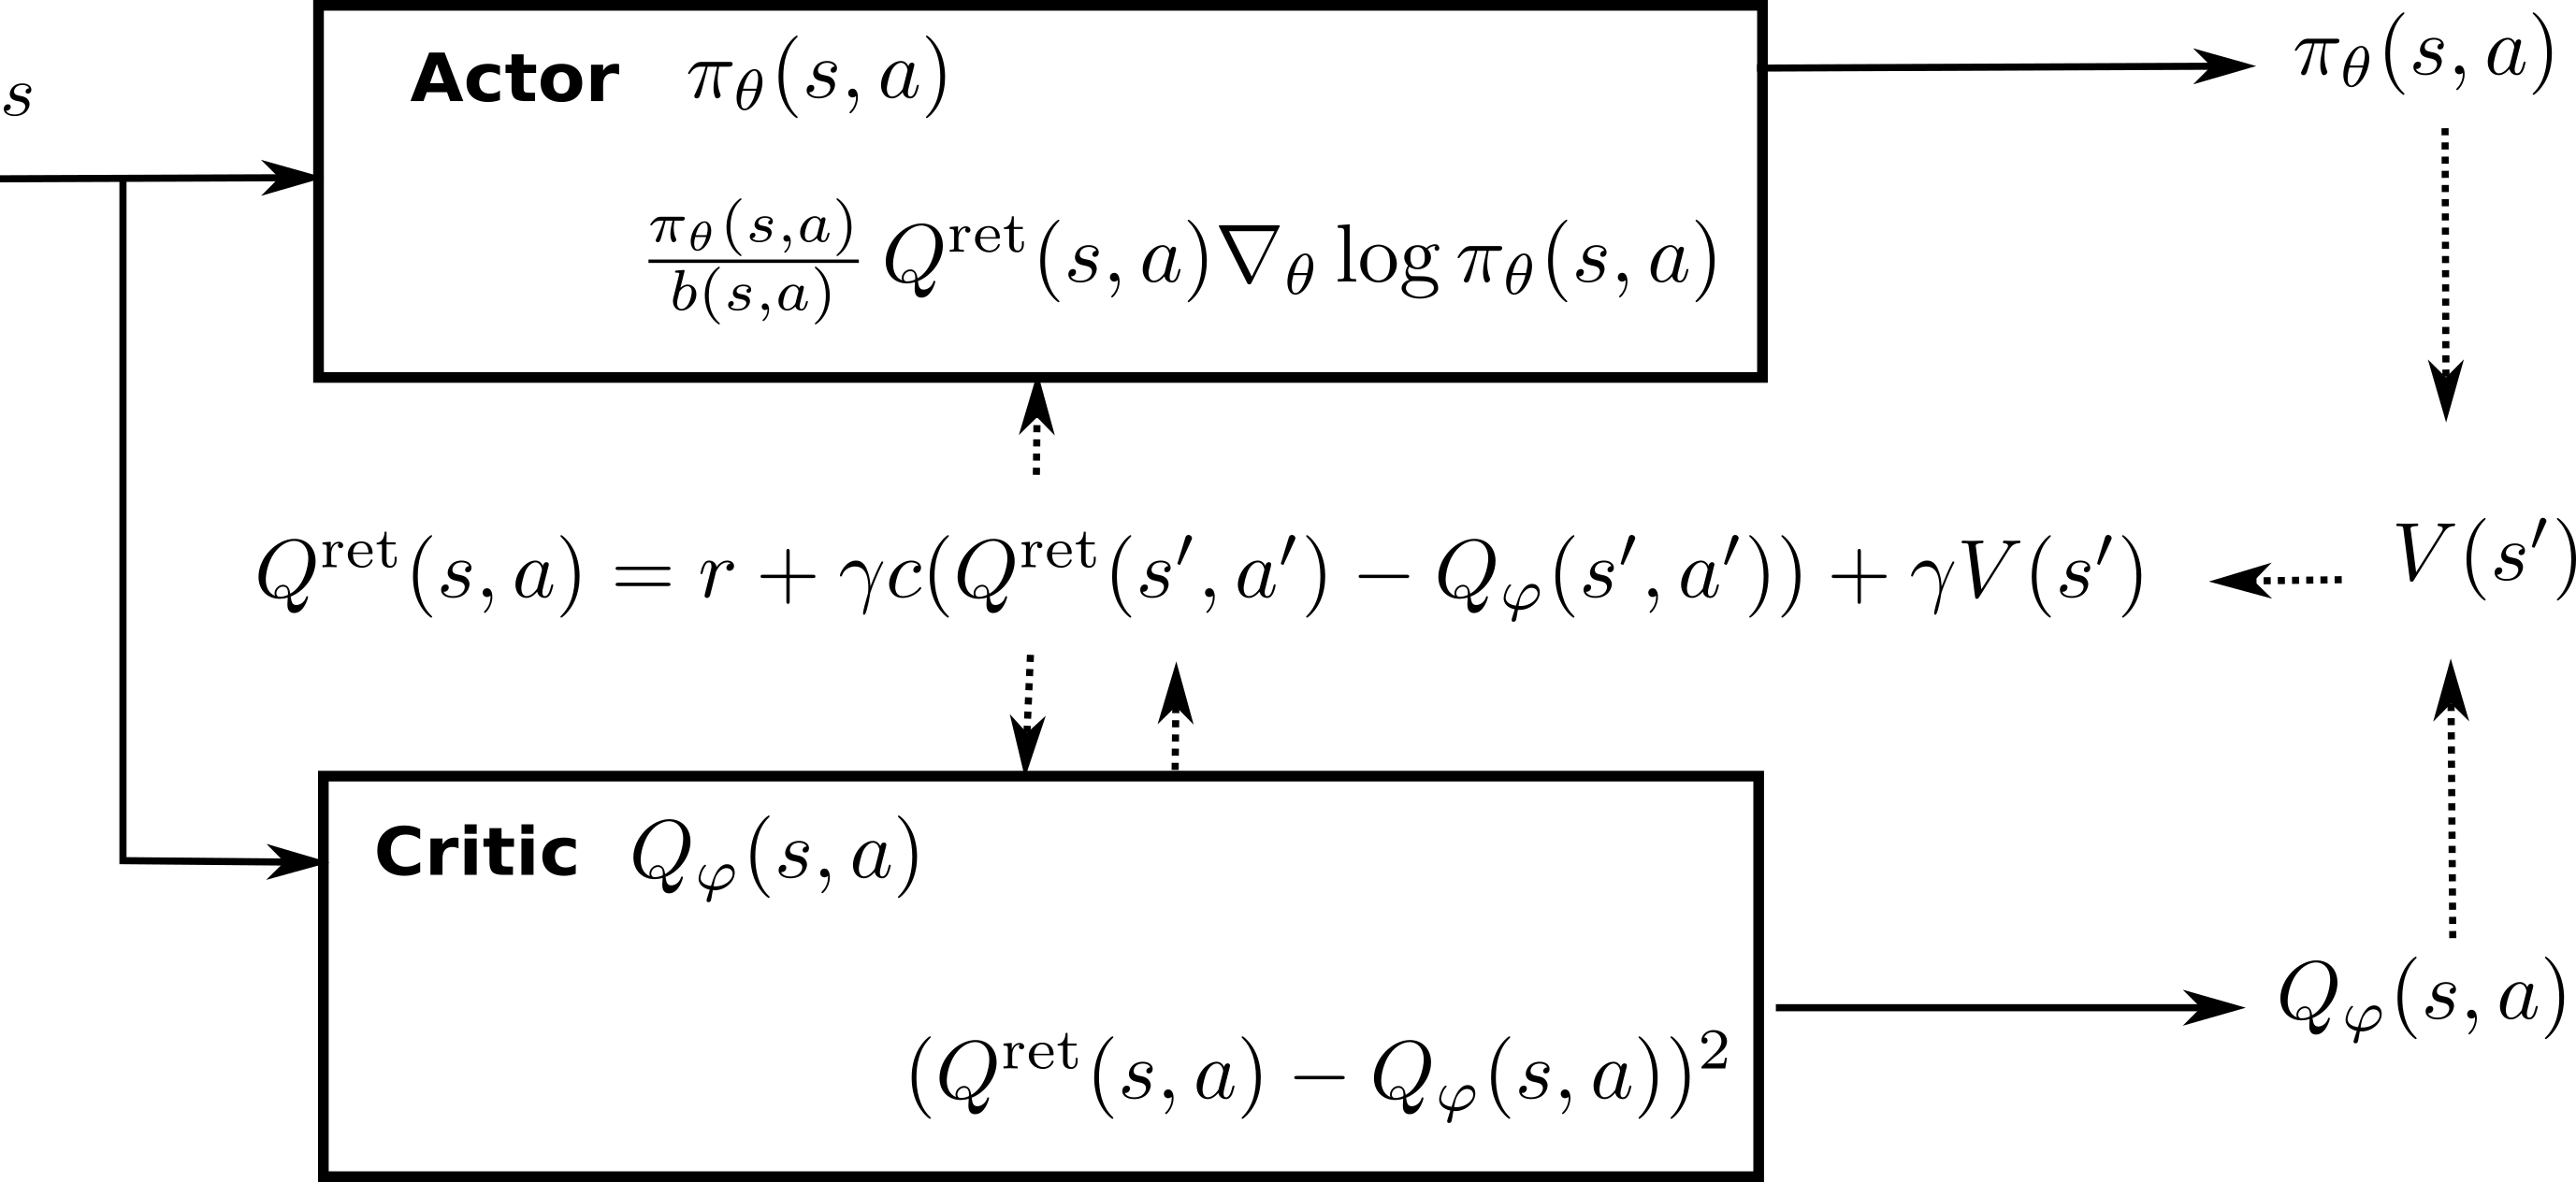
\includegraphics[width=0.9\textwidth,height=\textheight]{./img/acer.png}

}

\caption{\label{fig-acer}Architecture of the ACER actor-critic.}

\end{figure}

The target Q-value \(Q^\text{ret}(s, a)\) can be found recursively by
iterating backwards over the episode:

\begin{center}\rule{0.5\linewidth}{0.5pt}\end{center}

\begin{itemize}
\item
  Initialize \(Q^\text{ret}(s_T, a_T)\), \(Q_\varphi(s_T, a_T)\) and
  \(V(s_T)\) to 0, as the terminal state has no value.
\item
  for \(t \in [T-1, \ldots, 0]\):

  \begin{itemize}
  \tightlist
  \item
    Update the target Q-value using the received reward, the critic and
    the previous target value:
  \end{itemize}

  \[
        Q^\text{ret}(s_t, a_t) = r_{t+1} + \gamma \, c_{t+1} \, (Q^\text{ret}(s_{t+1}, a_{t+1}) - Q_\varphi(s_{t+1}, a_{t+1})) + \gamma \, V(s_{t+1})
    \]

  \begin{itemize}
  \tightlist
  \item
    Apply the critic on the current action:
  \end{itemize}

  \[
        Q_\varphi(s_t, a_t)
    \]

  \begin{itemize}
  \tightlist
  \item
    Estimate the value of the state using the critic:
  \end{itemize}

  \[
        V(s_t) = \sum_a \pi_\theta(s_t) \, Q_\varphi(s_t, a)
    \]
\end{itemize}

\begin{center}\rule{0.5\linewidth}{0.5pt}\end{center}

As the target value \(Q^\text{ret}(s, a)\) use multiple ``real'' rewards
\(r_{t+1}\), it is actually less biased than the critic
\(Q_\varphi(s, a)\). It is then better to use it to update the actor:

\[
    \nabla_\theta J(\theta)  = \mathbb{E}_{s_t, a_t \sim \rho_b} [\frac{\pi_\theta(s_t, a_t)}{b(s_t, a_t)} \, Q^\text{ret}(s_t, a_t) \, \nabla_\theta \log \pi_\theta(s_t, a_t)]
\]

The critic just has to minimize the mse with the target value:

\[
    \mathcal{L}(\varphi) = \mathbb{E}_{s_t, a_t \sim \rho_b} [(Q^\text{ret}(s, a) - Q_\varphi(s, a))^2]
\]

\hypertarget{importance-weight-truncation-with-bias-correction}{%
\subsubsection*{Importance weight truncation with bias
correction}\label{importance-weight-truncation-with-bias-correction}}
\addcontentsline{toc}{subsubsection}{Importance weight truncation with
bias correction}

When updating the actor, we rely on the importance sampling weight
\(\rho_t = \frac{\pi_\theta(s_t, a_t)}{b(s_t, a_t)}\) which can vary a
lot and destabilize learning.

\[
    \nabla_\theta J(\theta)  = \mathbb{E}_{s_t, a_t \sim \rho_b} [\rho_t \, Q^\text{ret}(s_t, a_t) \, \nabla_\theta \log \pi_\theta(s_t, a_t)]
\]

PPO solved this problem by clipping the importance sampling weight
between \(1- \epsilon\) and \(1+\epsilon\). ACER uses a similar
strategy, but only using an upper bound \(c = 10\) on the weight:

\[
    \bar{\rho}_t = \min(c, \rho_t)
\]

Using \(\bar{\rho}_t\) in the policy gradient directly would introduce a
bias: actions whose importance sampling weight \(\rho_t\) is higher than
\(c\) would contribute to the policy gradient with a smaller value than
they should, introducing a bias.

The solution in ACER is to add a \textbf{bias correcting term}, that
corrects the policy gradient when an action has a weight higher than
\(c\):

\[
\begin{aligned}
    \nabla_\theta J(\theta)  = & \mathbb{E}_{s_t \sim \rho_b} [\mathbb{E}_{a_t \sim b} [\bar{\rho}_t \, Q^\text{ret}(s_t, a_t) \, \nabla_\theta \log \pi_\theta(s_t, a_t)] \\
    & + \mathbb{E}_{a \sim \pi_\theta}[(\frac{\rho_t(a) - c}{\rho_t(a)})^+ \, Q_\varphi(s_t, a) \, \nabla_\theta \log \pi_\theta(s_t, a)]] \\
\end{aligned}
\]

The left part of that equation is the same policy gradient as before,
but using a clipped importance sampling weight.

The right part requires to integrate over all possible actions in the
state \(s_t\) according to the learned policy \(\pi_\theta\), although
only the action \(a_t\) was selected by the behavior policy \(b\). The
term \((\frac{\rho_t(a) - c}{\rho_t(a)})^+\) is zero for all actions
having an importance sampling weight smaller than c, and has a maximum
of 1. In practice, this correction term can be computed using the
vectors \(\pi_\theta(s, a)\) and \(Q_\varphi(s, a)\), which are the
outputs of the actor and the critic, respectively.

Finally, the Q-values \(Q^\text{ret}(s_t, a_t)\) and
\(Q_\varphi(s_t, a)\) are transformed into advantages
\(Q^\text{ret}(s_t, a_t) - V_\varphi(s_t)\) and
\(Q_\varphi(s_t, a) - V_\varphi(s_t)\) by substracting the value of the
state in order to reduce the variance of the policy gradient.

In short, we now have an estimator of the policy gradient which is
\textbf{unbiased} and of smaller variance.

\hypertarget{efficient-trust-region-policy-optimization}{%
\subsubsection*{Efficient trust region policy
optimization}\label{efficient-trust-region-policy-optimization}}
\addcontentsline{toc}{subsubsection}{Efficient trust region policy
optimization}

However, the variance is still too high. The last important step of ACER
is an efficient TRPO update for the parameters of the actor.

A first component of their TRPO update is they use a \textbf{target
actor network} \(\theta'\) (called averaged policy network in the paper)
slowly tracking the actor \(\theta\) after each update:

\[
    \theta' \leftarrow \alpha \, \theta' + (1 - \alpha) \, \theta
\]

A second component is that the actor is decomposed into two components:

\begin{enumerate}
\def\labelenumi{\arabic{enumi}.}
\tightlist
\item
  a distribution \(f\).
\item
  the statistics \(\Phi_\theta(x)\) of this distribution.
\end{enumerate}

This is what you do when you apply the softmax action selection on
Q-values: the distribution is the Gibbs (or Boltzmann) distribution and
the Q-values are its statistics. In the discrete case, they take a
categorical (or multinouilli) distribution: \(\Phi_\theta(s)\) is the
probability for each action to be taken and the distribution selects one
of them. Think of a dice with one side per action and probabilities
governed by the policy. In the continuous case, it could be anything,
for example a normal distribution.

Let's rewrite the policy gradient with that formulation (we omit here
the bias correction, but ACER uses it), but only w.r.t the output of the
actor \(\Phi_\theta(s_t)\) for a state \(s_t\):

\[
    \hat{g_t}^\text{ACER} = \nabla_{\Phi_\theta(s_t)} J(\theta)  = \bar{\rho}_t \, (Q^\text{ret}(s_t, a_t) - V_\phi(s_t) ) \, \nabla_{\Phi_\theta(s_t)} \log f(a_t | \Phi_\theta(s_t))
\]

To compute the policy gradient, we would only need to apply the chain
rule:

\[
    \nabla_\theta J(\theta) = \mathbb{E}_{s_t, a_t \sim \rho_b} [ \hat{g_t}^\text{ACER} \, \nabla_\theta \Phi_\theta(s_t) ]
\]

The variance of \(\hat{g_t}^\text{ACER}\) is too high. ACER defines the
following TRPO problem: we search for a gradient \(z\) solution of:

\[
    \min_z ||\hat{g_t}^\text{ACER} - z ||^2 \\
    \text{s.t.} \quad \nabla_{\Phi_\theta(s_t)} D_{KL}( f(\cdot | \Phi_{\theta'}(s_t) ) || f(\cdot | \Phi_{\theta'}(s_t)) )^T \times z < \delta
\]

The exact meaning of the constraint is hard to grasp, but here some
intuition: the change of policy \(z\) (remember that
\(\hat{g_t}^\text{ACER}\) is defined w.r.t the output of the actor)
should be as orthogonal as possible (within a margin \(\delta\)) to the
change of the \textbf{Kullback-Leibler} divergence between the policy
defined by the actor (\(\theta\)) and the one defined by the
\textbf{target actor} (\(\theta'\)). In other words, we want to update
the actor, but without making the new policy too different from its past
values (the target actor).

The advantage of this formulation is that the objective function is
quadratic in \(z\) and the constraint is linear. We can therefore very
easily find its solution using KKT optimization:

\[
    z^* = \hat{g_t}^\text{ACER} - \max(0, \frac{k^T \, \hat{g_t}^\text{ACER} - \delta}{||k||^2}) \, k
\]

where
\(k = \nabla_{\Phi_\theta(s_t)} D_{KL}( f(\cdot | \Phi_{\theta'}(s_t) ) || f(\cdot | \Phi_{\theta'}(s_t)) )\).

Having obtained \(z^*\), we can safely update the parameters of the
actor in the direction of:

\[
    \nabla_\theta J(\theta) = \mathbb{E}_{s_t, a_t \sim \rho_b} [ z^* \, \nabla_\theta \Phi_\theta(s_t) ]
\]

As noted in the paper: \emph{``The trust region step is carried out in
the space of the statistics of the distribution \(f\) , and not in the
space of the policy parameters. This is done deliberately so as to avoid
an additional back-propagation step through the policy network''}. We
indeed need only one network update per transition. If the KL divergence
was computed with respect to \(\pi_\theta\) directly, one would need to
apply backpropagation on the target network too.

The target network \(\theta'\) is furthermore used as the behavior
policy \(b(s, a)\). here is also a \textbf{target critic network}
\(\varphi'\), which is primarily used to compute the value of the states
\(V_{\varphi'}(s)\) for variance reduction.

For a complete description of the algorithm, refer to the paper\ldots{}
To summarize, ACER is an actor-critic architecture using Retrace
estimated values, importance weight truncation with bias correction and
efficient TRPO. Its variant for continuous action spaces furthermore
uses a \textbf{Stochastic Dueling Network} (SDN) in order estimate both
\(Q_\varphi(s, a)\) and \(V_\varphi(s)\). It is straightforward in the
discrete case (multiply the policy with the Q-values and take the
average) but hard in the continuous case.

ACER improved the performance and/or the sample efficiency of the
state-of-the-art (A3C, DDPG, etc) on a variety of tasks (Atari, Mujoco).
Apart from truncation with bias correction, all aspects of the algorithm
are essential to obtain this improvement, as shown by ablation studies.

\bookmarksetup{startatroot}

\hypertarget{maximum-entropy-rl}{%
\chapter{Maximum Entropy RL}\label{maximum-entropy-rl}}

All the methods seen sofar focus on finding a policy (or value
functions) that maximizes the obtained return. This corresponds to the
\textbf{exploitation} part of RL: we care only about the optimal policy.
The \textbf{exploration} is ensured by external mechanisms, such as
\(\epsilon\)-greedy or softmax policies in value based methods, or
adding exploratory noise to the actions as in DDPG. Exploration
mechanisms typically add yet another free parameter (\(\epsilon\),
softmax temperature, etc) that additionally need to be scheduled (more
exploration at the beginning of learning than at the end).

The idea behind \textbf{maximum entropy RL} is to let the algorithm
learn by itself how much exploration it needs to learn appropriately.
There are several approaches to this problem (see for example (Machado
et al., 2018) for an approach using successor representations), we focus
first on methods using \textbf{entropy regularization}, a concept
already seen briefly in A3C, before looking at soft methods such as Soft
Q-learning and SAC.

\hypertarget{entropy-regularization-1}{%
\subsection{Entropy regularization}\label{entropy-regularization-1}}

\textbf{Entropy regularization} (Williams and Peng, 1991) adds a
regularization term to the objective function:

\begin{equation}\protect\hypertarget{eq-entropy_reg}{}{
    J(\theta) =  \mathbb{E}_{s_t \sim \rho^\pi, a_t \sim \pi_\theta}[ R(s_t, a_t) + \beta \,  H(\pi_\theta(s_t))]
}\label{eq-entropy_reg}\end{equation}

We will neglect here how the objective function is sampled (policy
gradient, etc.) and focus on the second part.

The entropy of a discrete policy \(\pi_\theta\) in a state \(s_t\) is
given by:

\[
    H(\pi_\theta(s_t)) = - \sum_a \pi_\theta(s_t, a) \, \log \pi_\theta(s_t, a)
\]

For continuous actions, one can replace the sum with an integral. The
entropy of the policy measures its ``randomness'':

\begin{itemize}
\tightlist
\item
  if the policy is fully deterministic (the same action is
  systematically selected), the entropy is zero as it carries no
  information.
\item
  if the policy is completely random (all actions are equally
  surprising), the entropy is maximal.
\end{itemize}

By adding the entropy as a regularization term directly to the objective
function, we force the policy to be as non-deterministic as possible,
i.e.~to explore as much as possible, while still getting as many rewards
as possible. The parameter \(\beta\) controls the level of
regularization: we do not want the entropy to dominate either, as a
purely random policy does not bring much reward. If \(\beta\) is chosen
too low, the entropy won't play a significant role in the optimization
and we may obtain a suboptimal deterministic policy early during
training as there was not enough exploration. If \(\beta\) is too high,
the policy will be random and suboptimal.

Besides exploration, why would we want to learn a stochastic policy,
while the solution to the Bellman equations is deterministic by
definition? A first answer is that we rarely have a MDP: most
interesting problems are POMDP, where the states are indirectly inferred
through observations, which can be probabilistic. Todorov (2008) showed
that a stochastic policy emerges as the optimal answer when we consider
the connection between optimal control and probabilistic inference (see
also Toussaint, 2009).

Consider a two-opponents game like chess: if you have a deterministic
policy, you will always play the same moves in the same configuration.
In particular, you will always play the same opening moves. Your game
strategy becomes predictable for your opponent, who can adapt
accordingly. Having a variety of opening moves (as long as they are not
too stupid) is obviously a better strategy on the long term. This is due
to the fact that chess is actually a POMDP: the opponent's strategy and
beliefs are not accessible.

Another way to view the interest of entropy regularization is to realize
that learning a deterministic policy only leads to a single optimal
solution to the problem. Learning a stochastic policy forces the agent
to learn \textbf{many} optimal solutions to the same problem: the agent
is somehow forced to learn as much information as possible for the
experienced transitions, potentially reducing the sample complexity.

Entropy regularization is nowadays used very commonly used in deep RL
networks (e.g. O'Donoghue et al., 2016), as it is ``only'' an additional
term to set in the objective function passed to the NN, adding a single
hyperparameter \(\beta\).

\hypertarget{soft-q-learning}{%
\subsection{Soft Q-learning}\label{soft-q-learning}}

Entropy regularization greedily maximizes the entropy of the policy in
each state (the objective is the return plus the entropy in the current
state). Building on the maximum entropy RL framework (Nachum et al.,
2017; Schulman et al., 2017b; Ziebart et al., 2008), Haarnoja et al.
(2017) proposed a version of \textbf{soft-Q-learning} by extending the
definition of the objective:

\begin{equation}\protect\hypertarget{eq-softQ}{}{
    J(\theta) =  \sum_t \mathbb{E}_{s_t \sim \rho^\pi, a_t \sim \pi_\theta}[ r(s_t, a_t) + \beta \,  H(\pi_\theta(s_t))]
}\label{eq-softQ}\end{equation}

In this formulation based on trajectories, the agent seeks a policy that
maximizes the entropy of the complete trajectories rather than the
entropy of the policy in each state. This is a very important
distinction: the agent does not only search a policy with a high
entropy, but a policy that brings into states with a high entropy,
i.e.~where the agent is the most uncertain. This allows for very
efficient exploration strategies, where the agent will try to reduce its
uncertainty about the world and gather a lot more information than when
simply searching for a good policy.

Note that it is always possible to fall back to classical Q-learning by
setting \(\beta=0\) and that it is possible to omit this hyperparameter
by scaling the rewards with \(\frac{1}{\beta}\). The discount rate
\(\gamma\) is omitted here for simplicity, but it should be added back
when the task has an infinite horizon.

In soft Q-learning, the policy can be defined by a softmax over the soft
Q-values \(Q_\text{soft}(s, a)\), where \(\beta\) plays the role of the
temperature parameter:

\[
    \pi(s, a) \propto \exp(Q_\text{soft}(s_t, a_t) / \beta)
\]

Note that \(-Q_\text{soft}(s_t, a_t) / \beta\) plays the role of the
energy of the policy (as in Boltzmann machines), hence the name of the
paper (\emph{Reinforcement Learning with Deep Energy-Based Policies}).
We will ignore this analogy here. The normalization term of the softmax
(the log-partition function in energy-based models) is also omitted as
it later disappears from the equations anyway.

The soft Q-values are defined by the following Bellman equation:

\begin{equation}\protect\hypertarget{eq-softQ_update}{}{
    Q_\text{soft}(s_t, a_t) = r(s_t, a_t) + \gamma \, \mathbb{E}_{s_{t+1} \in \rho} [V_\text{soft}(s_{t+1})]
}\label{eq-softQ_update}\end{equation}

This is the regular Bellman equation that can be turned into an update
rule for the soft Q-values (minimizing the mse between the l.h.s and the
r.h.s). The soft value of a state is given by:

\begin{equation}\protect\hypertarget{eq-softV_update}{}{
    V_\text{soft}(s_t) = \mathbb{E}_{a_{t} \in \pi} [Q_\text{soft}(s_{t}, a_{t}) - \log \, \pi(s_t, a_t)]
}\label{eq-softV_update}\end{equation}

The notation in Haarnoja et al. (2017) is much more complex than that
(the paper includes the theoretical proofs), but it boils down to this
in Haarnoja et al. (2018b). When Equation~\ref{eq-softQ_update} is
applied repeatedly with the definition of
Equation~\ref{eq-softV_update}, it converges to the optimal solution of
Equation~\ref{eq-softQ}, at least in the tabular case.

The soft V-value of a state is the expectation of the Q-values in that
state (as in regular RL) minus the log probability of each action. This
last term measures the entropy of the policy in each state (when
expanding the expectation over the policy, we obtain \(- \pi \log \pi\),
which is the entropy).

In a nutshell, the soft Q-learning algorithm is:

\begin{itemize}
\tightlist
\item
  Sample transitions \((s, a, r, s')\) and store them in a replay
  memory.
\item
  For each transition \((s, a, r, s')\) in a minibatch of the replay
  memory:

  \begin{itemize}
  \tightlist
  \item
    Estimate \(V_\text{soft}(s')\) with Equation~\ref{eq-softV_update}
    by sampling several actions.
  \item
    Update the soft Q-value of \((s,a)\) with
    Equation~\ref{eq-softQ_update}.
  \item
    Update the policy (if not using the softmax over soft Q-values
    directly).
  \end{itemize}
\end{itemize}

The main drawback of this approach is that several actions have to be
sampled in the next state in order to estimate its current soft V-value,
what makes it hard to implement in practice. The policy also has to be
sampled from the Q-values, what is not practical for continuous action
spaces.

But the real interesting thing is the policies that are learned in
multi-goal settings, as in Figure~\ref{fig-softql}. The agent starts in
the middle of the environment and can obtain one of the four rewards
(north, south, west, east). A regular RL agent would very quickly select
only one of the rewards and stick to it. With soft Q-learning, the
policy stays stochastic and the four rewards can be obtained even after
convergence. This indicates that the soft agent has learned much more
about its environment than its hard equivalent, thanks to its maximum
entropy formulation.

\begin{figure}

{\centering 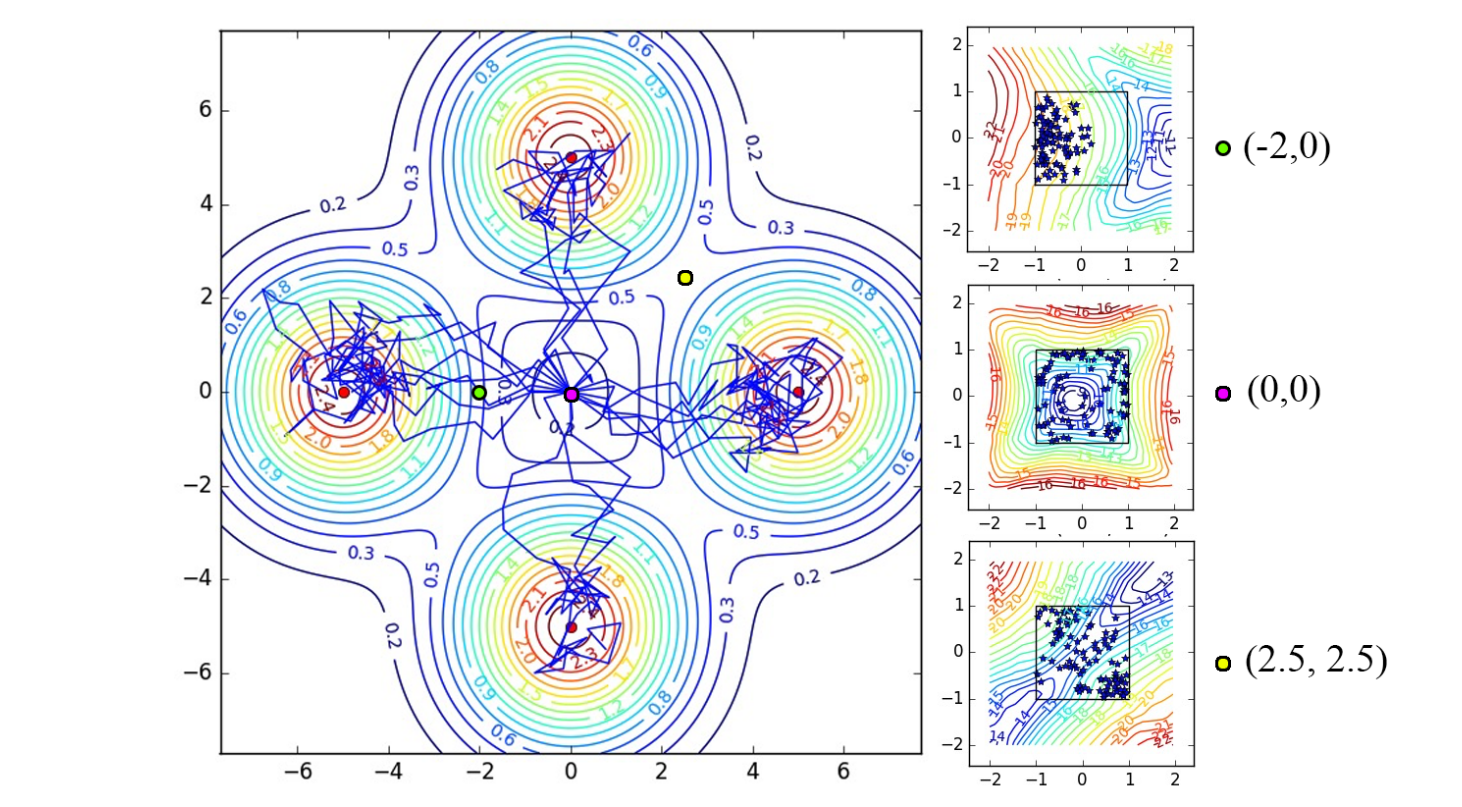
\includegraphics{./img/softQL.png}

}

\caption{\label{fig-softql}Policy learned by Soft Q-learning in a
multi-goal setting. Taken from Haarnoja et al. (2017).}

\end{figure}

\hypertarget{soft-actor-critic-sac}{%
\subsection{Soft Actor-Critic (SAC)}\label{soft-actor-critic-sac}}

Haarnoja et al. (2018b) proposed the \textbf{Soft Actor-Critic} (SAC),
an off-policy actor-critic which allows to have a stochastic actor
(contrary to DDPG) while being more optimal and sample efficient than
on-policy methods such as A3C or PPO. It is also less sensible to
hyperparameters than all these methods.

SAC builds on soft Q-learning to achieve these improvements. It relies
on three different function approximators:

\begin{itemize}
\tightlist
\item
  a soft state value function \(V_\varphi(s)\).
\item
  a soft Q-value function \(Q_\psi(s,a)\).
\item
  a stochastic policy \(\pi_\theta(s, a)\).
\end{itemize}

The paper uses a different notation for the parameters
\(\theta, \varphi, \psi\), but I choose to be consistent with the rest
of this document.

The soft state-value function \(V_\varphi(s)\) is learned using
Equation~\ref{eq-softV_update} which is turned into a loss function:

\[
    \mathcal{L}(\varphi) = \mathbb{E}_{s_t \in \mathcal{D}} [\mathbb{E}_{a_{t} \in \pi} [(Q_\psi(s_{t}, a_{t}) - \log \, \pi_\theta(s_t, a_t)] - V_\varphi(s_t) )^2]
\]

In practice, we only need the gradient of this loss function to train
the corresponding neural network. The expectation over the policy inside
the loss function can be replaced by a single sample action \(a\) using
the current policy \(\pi_\theta\) (but not \(a_{t+1}\) in the replay
memory \(\mathcal{D}\), which is only used for the states \(s_t\)).

\[
    \nabla_\varphi \mathcal{L}(\varphi) = \nabla_\varphi V_\varphi(s_t) \, (V_\varphi(s_t) - Q_\psi(s_{t}, a) + \log \, \pi_\theta(s_t, a) )
\]

The soft Q-values \(Q_\psi(s_{t}, a_{t})\) can be trained from the
replay memory \(\mathcal{D}\) on \((s_t, a_t, r_{t+1} , s_{t+1})\)
transitions by minimizing the mse:

\[
    \mathcal{L}(\psi) = \mathbb{E}_{s_t, a_t \in \mathcal{D}} [(r_{t+1} + \gamma \, V_\varphi(s_{t+1}) - Q_\psi(s_t, a_t))^2]
\]

Finally, the policy \(\pi_\theta\) can be trained to maximize the
obtained returns. There are many ways to do that, but Haarnoja et al.
(2018b) proposes to minimize the Kullback-Leibler (KL) divergence
between the current policy \(\pi_\theta\) and a softmax function over
the soft Q-values:

\[
    \mathcal{L}(\theta) = \mathbb{E}_{s_t \in \mathcal{D}} [D_\text{KL}(\pi_\theta(s, \cdot) | \frac{\exp Q_\psi(s_t, \cdot)}{Z(s_t)})]
\]

where \(Z\) is the partition function to normalize the softmax.
Fortunately, it disappears when using the reparameterization trick and
taking the gradient of this loss (see the paper for details).

There are additional tricks to make it more efficient and robust, such
as target networks or the use of two independent function approximators
for the soft Q-values in order to reduce the bias, but the gist of the
algorithm is the following:

\begin{center}\rule{0.5\linewidth}{0.5pt}\end{center}

\begin{itemize}
\tightlist
\item
  Sample a transition \((s_t, a_t, r_{t+1}, a_{t+1})\) using the current
  policy \(\pi_\theta\) and store it in the replay memory
  \(\mathcal{D}\).
\item
  For each transition \((s_t, a_t, r_{t+1}, a_{t+1})\) of a minibatch of
  \(\mathcal{D}\):

  \begin{itemize}
  \tightlist
  \item
    Sample an action \(a \in \pi_\theta(s_t, \cdot)\) from the current
    policy.
  \item
    Update the soft state-value function \(V_\varphi(s_t)\): \[
      \nabla_\varphi \mathcal{L}(\varphi) = \nabla_\varphi V_\varphi(s_t) \, (V_\varphi(s_t) - Q_\psi(s_{t}, a) + \log \, \pi_\theta(s_t, a) )
      \]
  \item
    Update the soft Q-value function \(Q_\psi(s_t, a_t)\): \[
      \nabla_\psi \mathcal{L}(\psi) = - \nabla_\psi Q_\psi(s_t, a_t) \, (r_{t+1} + \gamma \, V_\varphi(s_{t+1}) - Q_\psi(s_t, a_t))
      \]
  \item
    Update the policy \(\pi_\theta(s_t, \cdot)\): \[
      \nabla_\theta \mathcal{L}(\theta) = \nabla_\theta D_\text{KL}(\pi_\theta(s, \cdot) | \frac{\exp Q_\psi(s_t, \cdot)}{Z(s_t)})
      \]
  \end{itemize}
\end{itemize}

\begin{center}\rule{0.5\linewidth}{0.5pt}\end{center}

SAC was compared to DDPG, PPO, soft Q-learning and others on a set of
gym and humanoid robotics tasks (with 21 joints!). It outperforms all
these methods in both the final performance and the sample complexity,
the difference being even more obvious for the complex tasks. The
exploration bonus given by the maximum entropy allows the agent to
discover better policies than its counterparts. SAC is an actor-critic
architecture (the critic computing both V and Q) working off-policy
(using an experience replay memory, so re-using past experiences)
allowing to learn stochastic policies, even in high dimensional spaces.

\bookmarksetup{startatroot}

\hypertarget{distributional-learning}{%
\chapter{Distributional learning}\label{distributional-learning}}

All RL methods based on the Bellman equations use the expectation
operator to average returns and compute the values of states and
actions:

\[
    Q^\pi(s, a) = \mathbb{E}_{s, a \sim \pi}[R(s, a)]
\]

The variance of the returns is not considered in the action selection
scheme, and most methods actually try to reduce this variance as it
impairs the convergence of neural networks. Decision theory states that
only the mean should matter on the long-term, but one can imagine tasks
where the variance is an important factor for the decision. Imagine you
are in a game where you have two actions available: the first one brings
returns of 10 and 20, with a probability of 0.5 each (to simplify),
while the second one brings returns of -10 and +40 with probability 0.5
too. Both actions have the same Q-value of 15 (a return which is
actually never experienced), so one can theoretically pick whatever
action, both are optimal in the Bellman's sense.

However, this is only true when playing \textbf{long enough}. If, after
learning, one is only allowed one try on that game, it is obviously
safer (but less fun) to choose the first action, as one wins at worse
10, while it is -10 with the second action. Knowing the distribution of
the returns can allow to distinguish risky choices from safe ones more
easily and adapt the behavior. Another advantage would be that by
learning the distribution of the returns instead of just their mean, one
actually gathers more information about the environment dynamics: it can
only help the convergence of the algorithm towards the optimal policy.

\hypertarget{categorical-dqn}{%
\subsection{Categorical DQN}\label{categorical-dqn}}

Bellemare et al. (2017) proposed to learn the \textbf{value
distribution} (the probability distribution of the returns) through a
modification of the Bellman equation. They show that learning the
complete distribution of rewards instead of their mean leads to
performance improvements on Atari games over modern variants of DQN.

Their proposed \textbf{categorical DQN} (also called C51) has an
architecture based on DQN, but where the output layer predicts the
distribution of the returns for each action \(a\) in state \(s\),
instead of its mean \(Q^\pi(s, a)\). In practice, each action \(a\) is
represented by \(N\) output neurons, who encode the support of the
distribution of returns. If the returns take values between
\(V_\text{min}\) and \(V_\text{max}\), one can represent their
distribution \(\mathcal{Z}\) by taking \(N\) discrete ``bins'' (called
\emph{atoms} in the paper) in that range.
Figure~\ref{fig-distributionallearning} shows how the distribution of
returns between -10 and 10 can be represented using 21 atoms.

\begin{figure}

{\centering 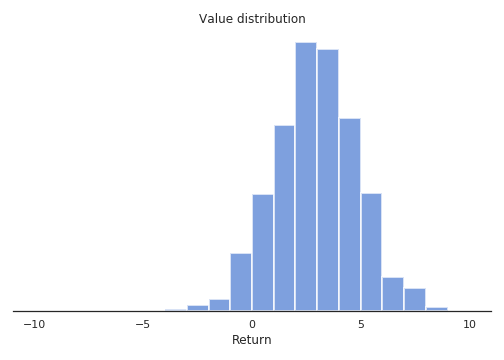
\includegraphics[width=0.8\textwidth,height=\textheight]{./img/distributionallearning.png}

}

\caption{\label{fig-distributionallearning}Example of a value
distribution using 21 atoms between -10 and 10. The average return is 3,
but its variance is explicitly represented.}

\end{figure}

Of course, the main problem is to know in advance the range of returns
\([V_\text{min}, V_\text{max}]\) (it depends largely on the choice of
the discount rate \(\gamma\)), but you can infer it from training
another algorithm such as DQN beforehand. Dabney et al. (2017) got rid
of this problem with quantile regression. In the paper, the authors
found out experimentally that 51 is the most efficient number of atoms
(hence the name C51).

Let's note \(z_i\) these atoms with \(1 \leq i < N\). The atom
probability that the return associated to a state-action pair \((s, a)\)
lies within the bin associated to the atom \(z_i\) is noted
\(p_i(s, a)\). These probabilities can be predicted by a neural network,
typically by using a softmax function over outputs
\(f_i(s, a; \theta)\):

\[
    p_i(s, a; \theta) = \frac{\exp f_i(s, a; \theta)}{\sum_{j=1}^{N} \exp f_j(s, a; \theta)}
\]

The distribution of the returns \(\mathcal{Z}\) is simply a sum over the
atoms (represented by the Dirac distribution \(\delta_{z_i}\)):

\[
    \mathcal{Z}_\theta(s, a) = \sum_{i=1}^{N} p_i(s, a; \theta) \, \delta_{z_i}
\]

If these probabilities are correctly estimated, the Q-value is easy to
compute as the mean of the distribution:

\[
    Q_\theta(s, a) = \mathbb{E} [\mathcal{Z}_\theta(s, a)] = \sum_{i=1}^{N} p_i(s, a; \theta) \, z_i
\]

These Q-values can then be used for action selection as in the regular
DQN. The problem is now to learn the value distribution
\(\mathcal{Z}_\theta\), i.e.~to find a learning rule / loss function for
the \(p_i(s, a; \theta)\). Let's consider a single transition
\((s, a, r, s')\) and select the greedy action \(a'\) in \(s'\) using
the current policy \(\pi_\theta\). The value distribution
\(\mathcal{Z}_\theta\) can be evaluated by applying recursively the
Bellman operator \(\mathcal{T}\):

\[
    \mathcal{T} \, \mathcal{Z}_\theta(s, a) = \mathcal{R}(s, a) + \gamma \, \mathcal{Z}_\theta(s', a')
\]

where \(\mathcal{R}(s, a)\) is the distribution of immediate rewards
after \((s, a)\). This use of the Bellman operator is the same as in
Q-learning:

\[
    \mathcal{T} \, \mathcal{Q}_\theta(s, a) = \mathbb{E}[r(s, a)] + \gamma \, \mathcal{Q}_\theta(s', a')
\]

In Q-learning, one minimizes the difference (mse) between
\(\mathcal{T} \, \mathcal{Q}_\theta(s, a)\) and
\(\mathcal{Q}_\theta(s, a)\), which are expectations (so we only
manipulate scalars). Here, we will minimize the statistical distance
between the distributions \(\mathcal{T} \, \mathcal{Z}_\theta(s, a)\)
and \(\mathcal{Z}_\theta(s, a)\) themselves, using for example the KL
divergence, Wasserstein metric, total variation or whatnot.

The problem is mostly that the distributions
\(\mathcal{T} \, \mathcal{Z}_\theta(s, a)\) and
\(\mathcal{Z}_\theta(s, a)\) do not have the same support: for a
particular atom \(z_i\), \(\mathcal{T} \, \mathcal{Z}_\theta(s, a)\) can
have a non-zero probability \(p_i(s, a)\), while
\(\mathcal{Z}_\theta(s, a)\) has a zero probability. Besides, the
probabilities must sum to 1, so one cannot update the \(z_i\)
independently from one another.

The proposed method consists of three steps:

\begin{enumerate}
\def\labelenumi{\arabic{enumi}.}
\tightlist
\item
  Computation of the Bellman update
  \(\mathcal{T} \, \mathcal{Z}_\theta(s, a)\). They simply compute
  translated values for each \(z_i\) according to:
\end{enumerate}

\[
    \mathcal{T} \, z_i = r + \gamma \, z_i
\]

and clip the obtained value to \([V_\text{min}, V_\text{max}]\). The
reward \(r\) translates the distribution of atoms, while the discount
rate \(\gamma\) scales it. Figure~\ref{fig-distributionallearning2}
shows the distribution of \(\mathcal{T} \, \mathcal{Z}_\theta(s, a)\)
compared to \(\mathcal{Z}_\theta(s, a)\). Note that the atoms of the two
distributions are not aligned.

\begin{figure}

{\centering 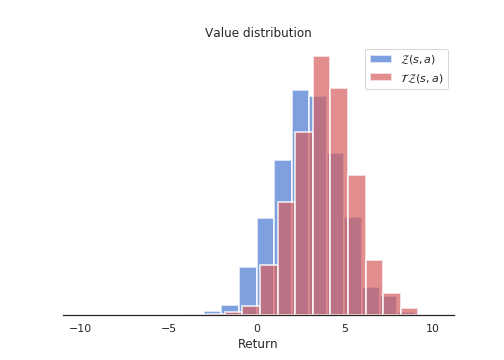
\includegraphics[width=0.8\textwidth,height=\textheight]{./img/distributionallearning2.png}

}

\caption{\label{fig-distributionallearning2}Computation of the Bellman
update \(\mathcal{T} \, \mathcal{Z}_\theta(s, a)\). The atoms of the two
distributions are not aligned.}

\end{figure}

\begin{enumerate}
\def\labelenumi{\arabic{enumi}.}
\setcounter{enumi}{1}
\tightlist
\item
  Distribution of the probabilities of
  \(\mathcal{T} \, \mathcal{Z}_\theta(s, a)\) on the support of
  \(\mathcal{Z}_\theta(s, a)\). The projected atom
  \(\mathcal{T} \, z_i\) lie between two ``real'' atoms \(z_l\) and
  \(z_u\), with a non-integer index \(b\) (for example \(b = 3.4\),
  \(l = 3\) and \(u=4\)). The corresponding probability
  \(p_{b}(s', a'; \theta)\) of the next greedy action \((s', a')\) is
  ``spread'' to its neighbors through a local interpolation depending on
  the distances between \(b\), \(l\) and \(u\):
\end{enumerate}

\[
    \Delta p_{l}(s', a'; \theta) = p_{b}(s', a'; \theta) \, (b - u)
\] \[
    \Delta p_{u}(s', a'; \theta) = p_{b}(s', a'; \theta) \, (l - b)
\]

Figure~\ref{fig-distributionallearning3} shows how the projected update
distribution \(\Phi \, \mathcal{T} \, \mathcal{Z}_\theta(s, a)\) now
matches the support of \(\mathcal{Z}_\theta(s, a)\)

\begin{figure}

{\centering 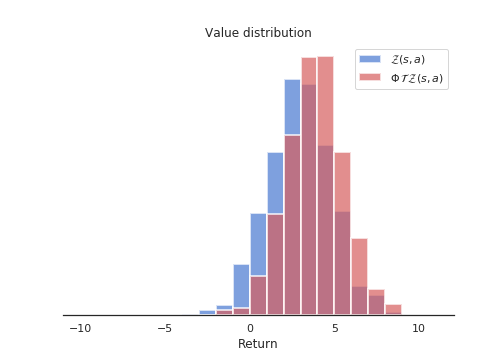
\includegraphics[width=0.8\textwidth,height=\textheight]{./img/distributionallearning3.png}

}

\caption{\label{fig-distributionallearning3}Projected update
\(\Phi \, \mathcal{T} \, \mathcal{Z}_\theta(s, a)\) on the support of
\(\mathcal{Z}_\theta(s, a)\). The atoms are now aligned, the statistical
distance between the two distributions can be minimized.}

\end{figure}

The projection of the Bellman update onto an atom \(z_i\) can be
summarized by the following equation:

\[
    (\Phi \, \mathcal{T} \, \mathcal{Z}_\theta(s, a))_i = \sum_{j=1}^N \big [1 - \frac{| [\mathcal{T}\, z_j]_{V_\text{min}}^{V_\text{max}} - z_i|}{\Delta z} \big ]_0^1 \, p_j (s', a'; \theta)
\]

where \([\cdot]_a^b\) bounds its argument in \([a, b]\) and \(\Delta z\)
is the step size between two atoms.

\begin{enumerate}
\def\labelenumi{\arabic{enumi}.}
\setcounter{enumi}{2}
\tightlist
\item
  Minimizing the statistical distance between
  \(\Phi \, \mathcal{T} \, \mathcal{Z}_\theta(s, a)\) and
  \(\mathcal{Z}_\theta(s, a)\). Now that the Bellman update has the same
  support as the value distribution, we can minimize the KL divergence
  between the two for a single transition:
\end{enumerate}

\[
    \mathcal{L}(\theta) = D_\text{KL} (\Phi \, \mathcal{T} \, \mathcal{Z}_{\theta'}(s, a) | \mathcal{Z}_\theta(s, a))
\]

using a target network \(\theta'\) for the target. It is to be noted
that minimizing the KL divergence is the same as minimizing the
cross-entropy between the two, as in classification tasks:

\[
    \mathcal{L}(\theta) =  - \sum_i (\Phi \, \mathcal{T} \, \mathcal{Z}_{\theta'}(s, a))_i \log p_i (s, a; \theta)
\]

The projected Bellman update plays the role of the one-hot encoded
target vector in classification (except that it is not one-hot encoded).
DQN performs a regression on the Q-values (mse loss), while categorical
DQN performs a classification (cross-entropy loss). Apart from the way
the target is computed, categorical DQN is very similar to DQN:
architecture, experience replay memory, target networks, etc.

Figure~\ref{fig-categoricaldqn} illustrates how the predicted value
distribution changes when playing Space invaders (also have a look at
the Youtube video at \url{https://www.youtube.com/watch?v=yFBwyPuO2Vg}).
C51 outperforms DQN on most Atari games, both in terms of the achieved
performance and the sample complexity.

\begin{figure}

{\centering \includegraphics[width=1\textwidth,height=\textheight]{./img/categoricaldqn.gif}

}

\caption{\label{fig-categoricaldqn}Evolution of the value distribution
for the categorical DQN playing Space Invaders. Animation taken from
\url{https://deepmind.com/blog/going-beyond-average-reinforcement-learning/}}

\end{figure}

\textbf{Additional resources:}

\begin{itemize}
\tightlist
\item
  \url{https://deepmind.com/blog/going-beyond-average-reinforcement-learning}
\item
  \url{https://physai.sciencesconf.org/data/pages/distributional_RL_Remi_Munos.pdf}
\item
  \url{https://flyyufelix.github.io/2017/10/24/distributional-bellman.html},
  with keras code for C51.
\end{itemize}

\hypertarget{the-reactor}{%
\subsection{The Reactor}\label{the-reactor}}

The \textbf{Reactor} (Retrace Actor) of Gruslys et al. (2017) combines
many architectural and algorithmic contributions seen until now in order
to provide an algorithm that is both sample efficient and with a good
run-time performance. A3C has for example a better run-time performance
(smaller wall-clock time for the training) than DQN or categorical DQN
thanks to the use of multiple actor-learners in parallel, but its sample
complexity is actually higher (as it is on-policy).

The Reactor combines and improves on:

\begin{itemize}
\tightlist
\item
  An actor-critic architecture using policy gradient with importance
  sampling,
\item
  Off-policy corrected returns computed by the Retrace algorithm,
\item
  Distributional learning of the Q-values in the critic,
\item
  Prioritized experience replay for sequences.
\end{itemize}

One could consider REACTOR as the distributional version of ACER. We
will not go into all the details here, but simply outline the main
novelties.

The Reactor is composed of an actor \(\pi_\theta(s, a)\) and a critic
\(Q_\varphi(s, a)\). The actor is trained using policy gradient with
importance sampling, as in Off-PAC. For a single state \(s\) and an
action \(\hat{a}\) sampled by the behavior policy \(b\), the gradient of
the objective is defined as:

\[
\begin{aligned}
    \nabla_\theta J(\theta) = \frac{\pi_\theta(s, \hat{a})}{b(s, \hat{a})} & \, (R(s, \hat{a}) - Q_\varphi(s, \hat{a})) \, \nabla_\theta \log \pi_\theta(s, \hat{a}) \\
    & + \sum_a Q_\varphi(s, a) \, \nabla_\theta \pi_\theta(s, a) \\
\end{aligned}
\]

The first term comes from Off-PAC and only concerns the chosen action
\(\hat{a}\) from the behavior policy. The actual return \(R(s, a)\) is
compared to its estimate \(Q_\varphi(s, \hat{a})\) in order to reduce
its variance. The second term
\(\sum_a Q_\varphi(s, a) \, \nabla_\theta \pi_\theta(s, a)\) depends on
all available actions in \(s\). Its role is to reduce the bias of the
first term, without adding any variance as it is only based on
estimates. As the value of the state is defined by
\(V^\pi(s) = \sum_a \pi(s, a) \, Q^\pi(s, a)\), maximizing this term
maximizes the value of the state, i.e.~the associated returns. This rule
is called \textbf{leave-one-out} (LOO), as one action is left out from
the sum and estimated from actual returns instead of other estimates.

For a better control on the variance, the behavior probability
\(b(s, a)\) is replaced by a parameter \(\beta\):

\[
    \nabla_\theta J(\theta) = \beta \, (R(s, \hat{a}) - Q_\varphi(s, \hat{a})) \, \nabla_\theta \pi_\theta(s, \hat{a}) + \sum_a Q_\varphi(s, a) \, \nabla_\theta \pi_\theta(s, a)
\]

\(\beta\) is defined as \(\min (c, \frac{1}{b(s, \hat{a})})\), where
\(c>1\) is a constant. This truncated term is similar to what was used
in ACER. The rule is now called \textbf{\(\beta\)-LOO} and is a novel
proposition of the Reactor.

The second importance contribution of the Reactor is how to combine the
Retrace algorithm (Munos et al. (2016)) for estimating the return
\(R(s, \hat{a})\) on multiple steps, with the distributional learning
method of Categorical DQN. As Retrace uses n-steps returns iteratively,
the n-step distributional Bellman target can updated using the \(n\)
future rewards:

\[
    z_i^n = \mathcal{T}^n \, z_i = \sum_{k=t}^{t+n} \gamma^{k-t} r_k + \gamma^n \, z_i
\]

We leave out the details on how Retrace is combined with these
distributional Bellman updates: the notation is complicated but the idea
is simple. The last importance contribution of the paper is the use of
\textbf{prioritized sequence replay}. Prioritized experience replay
allows to select in priority transitions from the replay buffer which
are the most surprising, i.e.~where the TD error is the highest. These
transitions are the ones carrying the most information. A similar
principle can be applied to sequences of transitions, which are needed
by the n-step updates. They devised a specific sampling algorithm in
order to achieve this and reduce the variance of the samples.

The last particularities of the Reactor is that it uses a LSTM layer to
make the problem Markovian (instead of stacking four frames as in DQN)
and train multiple actor-learners as in A3C. The algorithm is trained on
CPU, with 10 or 20 actor-learners. The Reactor outperforms DQN and its
variants, A3C and ACER on Atari games. Importantly, Reactor only needs
one day of training on CPU, compared to the 8 days of GPU training
needed by DQN.

\bookmarksetup{startatroot}

\hypertarget{miscellaneous-model-free-algorithm}{%
\chapter{Miscellaneous model-free
algorithm}\label{miscellaneous-model-free-algorithm}}

\hypertarget{stochastic-value-gradient-svg}{%
\subsection{Stochastic Value Gradient
(SVG)}\label{stochastic-value-gradient-svg}}

Heess et al. (2015)

\hypertarget{q-prop}{%
\subsection{Q-Prop}\label{q-prop}}

Gu et al. (2016b)

\hypertarget{normalized-advantage-function-naf}{%
\subsection{Normalized Advantage Function
(NAF)}\label{normalized-advantage-function-naf}}

Gu et al. (2016a)

\hypertarget{fictitious-self-play-fsp}{%
\subsection{Fictitious Self-Play (FSP)}\label{fictitious-self-play-fsp}}

Heinrich et al. (2015) Heinrich and Silver (2016)

\hypertarget{comparison-between-value-based-and-policy-gradient-methods}{%
\section{Comparison between value-based and policy gradient
methods}\label{comparison-between-value-based-and-policy-gradient-methods}}

Having now reviewed both value-based methods (DQN and its variants) and
policy gradient methods (A3C, DDPG, PPO), the question is which method
to choose? While not much happens right now for value-based methods,
policy gradient methods are attracting a lot of attention, as they are
able to learn policies in continuous action spaces, what is very
important in robotics.
\url{https://flyyufelix.github.io/2017/10/12/dqn-vs-pg.html} summarizes
the advantages and inconvenients of policy gradient methods.

Advantages of PG:

\begin{itemize}
\tightlist
\item
  Better convergence properties, more stable (Duan et al., 2016).
\item
  Effective in high-dimensional or continuous action spaces.
\item
  Can learn stochastic policies.
\end{itemize}

Disadvantages of PG:

\begin{itemize}
\tightlist
\item
  Typically converge to a local rather than global optimum.
\item
  Evaluating a policy is often inefficient and having a high variance.
\item
  Worse sample efficiency (but it is getting better).
\end{itemize}

\hypertarget{gradient-free-policy-search}{%
\section{Gradient-free policy
search}\label{gradient-free-policy-search}}

The policy gradient methods presented above rely on backpropagation and
gradient descent/ascent to update the parameters of the policy and
maximize the objective function. Gradient descent is generally slow,
sample inefficient and subject to local minima, but is nevertheless the
go-to method in neural networks. However, it is not the only
optimization that can be used in deep RL. This section presents quickly
some of the alternatives.

\hypertarget{cross-entropy-method-cem}{%
\subsection{Cross-entropy Method (CEM)}\label{cross-entropy-method-cem}}

Szita and Lörincz (2006)

\hypertarget{evolutionary-search-es}{%
\subsection{Evolutionary Search (ES)}\label{evolutionary-search-es}}

Salimans et al. (2017)

Explanations from OpenAI:
\url{https://blog.openai.com/evolution-strategies/}

Deep neuroevolution at Uber:
\url{https://eng.uber.com/deep-neuroevolution/}

\bookmarksetup{startatroot}

\hypertarget{recurrent-attention-models}{%
\chapter{Recurrent Attention Models}\label{recurrent-attention-models}}

\textbf{Work in progress}

Mnih et al. (2014), Ba et al. (2014). Stollenga et al. (2014)

\bookmarksetup{startatroot}

\hypertarget{model-based-rl}{%
\chapter{Model-based RL}\label{model-based-rl}}

\textbf{work in progress}

Model-free: The future is cached into values.

Two problems of model-free:

\begin{enumerate}
\def\labelenumi{\arabic{enumi}.}
\tightlist
\item
  Needs a lot of samples
\item
  Cannot adapt to novel tasks in the same environment.
\end{enumerate}

Model-based uses an internal model to reason about the future
(imagination).

Works only when the model is fixed (AlphaGo) or easy to learn (symbolic,
low-dimensional). Not robust yet against model imperfection.

\hypertarget{dyna-q}{%
\section{Dyna-Q}\label{dyna-q}}

(Sutton and Barto, 1990)

\url{https://medium.com/@ranko.mosic/online-planning-agent-dyna-q-algorithm-and-dyna-maze-example-sutton-and-barto-2016-7ad84a6dc52b}

\hypertarget{unsorted-references}{%
\section{Unsorted references}\label{unsorted-references}}

Embed to Control: A Locally Linear Latent Dynamics Model for Control
from Raw Images (Watter et al., 2015)

Efficient Model-Based Deep Reinforcement Learning with Variational State
Tabulation (Corneil et al., 2018)

Model-Based Value Estimation for Efficient Model-Free Reinforcement
Learning (Feinberg et al., 2018)

Imagination-Augmented Agents for Deep Reinforcement Learning (Weber et
al., 2017).

Temporal Difference Model TDM (Pong et al., 2018):
\url{http://bair.berkeley.edu/blog/2018/04/26/tdm/}

Learning to Adapt: Meta-Learning for Model-Based Control, (Clavera et
al., 2018)

The Predictron: End-To-End Learning and Planning (Silver et al., 2016b)

Model-Based Planning with Discrete and Continuous Actions (Henaff et
al., 2017)

Schema Networks: Zero-shot Transfer with a Generative Causal Model of
Intuitive Physics (Kansky et al., 2017)

Universal Planning Networks (Srinivas et al., 2018)

World models \url{https://worldmodels.github.io/} (Ha and Schmidhuber,
2018)

Recall Traces: Backtracking Models for Efficient Reinforcement Learning
(Goyal et al., 2018)

Deep Dyna-Q: Integrating Planning for Task-Completion Dialogue Policy
Learning (Peng et al., 2018)

Q-map: a Convolutional Approach for Goal-Oriented Reinforcement Learning
(Pardo et al., 2018)

\bookmarksetup{startatroot}

\hypertarget{hierarchical-reinforcement-learning}{%
\chapter{Hierarchical Reinforcement
Learning}\label{hierarchical-reinforcement-learning}}

\textbf{work in progress}

Very good link:
\url{https://thegradient.pub/the-promise-of-hierarchical-reinforcement-learning/}

Nachum et al. (2018)

Haarnoja et al. (2018a)

Co-Reyes et al. (2018)

\bookmarksetup{startatroot}

\hypertarget{inverse-reinforcement-learning}{%
\chapter{Inverse Reinforcement
Learning}\label{inverse-reinforcement-learning}}

\textbf{work in progress}

Hindsight experience replay: Andrychowicz et al. (2017)

Goal-conditioned inverse RL: Ding et al. (2019)

\bookmarksetup{startatroot}

\hypertarget{deep-rl-for-robotics}{%
\chapter{Deep RL for robotics}\label{deep-rl-for-robotics}}

\textbf{Work in progress}

Agrawal et al. (2016), Dosovitskiy and Koltun (2016), Gu et al. (2017),
Levine et al. (2016a), Levine et al. (2016b), Zhang et al. (2015)

Deep Reinforcement Learning for Industrial Insertion Tasks with Visual
Inputs and Natural Rewards (Schoettler et al., 2019)

State of the art: Amarjyoti (2017)

\bookmarksetup{startatroot}

\hypertarget{deep-rl-in-practice}{%
\chapter{Deep RL in practice}\label{deep-rl-in-practice}}

\hypertarget{limitations}{%
\section{Limitations}\label{limitations}}

Excellent blog post from Alex Irpan on the limitations of deep RL:
\url{https://www.alexirpan.com/2018/02/14/rl-hard.html}

Another documented critic on deep RL:
\url{https://thegradient.pub/why-rl-is-flawed/}

\hypertarget{simulation-environments}{%
\section{Simulation environments}\label{simulation-environments}}

Standard RL environments are needed to better compare the performance of
RL algorithms. Below is a list of the most popular ones, but refer to
\url{https://github.com/clvrai/awesome-rl-envs} for an up-to-date
curated list.

\begin{itemize}
\tightlist
\item
  OpenAI Gym \url{https://gym.openai.com}: a standard toolkit for
  comparing RL algorithms provided by the OpenAI foundation. It provides
  many environments, from the classical toy problems in RL (GridWorld,
  pole-balancing) to more advanced problems (Mujoco simulated robots,
  Atari games, Minecraft\ldots). The main advantage is the simplicity of
  the interface: the user only needs to select which task he wants to
  solve, and a simple for loop allows to perform actions and observe
  their consequences:
\end{itemize}

\begin{Shaded}
\begin{Highlighting}[]
\ImportTok{import}\NormalTok{ gym}
\NormalTok{env }\OperatorTok{=}\NormalTok{ gym.make(}\StringTok{"Taxi{-}v1"}\NormalTok{)}
\NormalTok{observation }\OperatorTok{=}\NormalTok{ env.reset()}
\ControlFlowTok{for}\NormalTok{ \_ }\KeywordTok{in} \BuiltInTok{range}\NormalTok{(}\DecValTok{1000}\NormalTok{):}
\NormalTok{    env.render()}
\NormalTok{    action }\OperatorTok{=}\NormalTok{ env.action\_space.sample()}
\NormalTok{    observation, reward, done, info }\OperatorTok{=}\NormalTok{ env.step(action)}
\end{Highlighting}
\end{Shaded}

\begin{itemize}
\item
  OpenAI Universe \url{https://universe.openai.com}: a similar framework
  from OpenAI, but to control realistic video games (GTA V, etc).
\item
  Darts environment \url{https://github.com/DartEnv/dart-env}: a fork of
  gym to use the Darts simulator instead of Mujoco.
\item
  Roboschool \url{https://github.com/openai/roboschool}: another
  alternative to Mujoco for continuous robotic control, this time from
  openAI.
\item
  NIPS 2017 musculo-skeletal challenge
  \url{https://github.com/stanfordnmbl/osim-rl}
\item
  Deepmind Lab \url{https://github.com/deepmind/lab}: a 3D learning
  environment based on id Software's Quake III Arena via ioquake3 and
  other open source software.
\item
  AnimalAI Olympics \url{https://github.com/beyretb/AnimalAI-Olympics},
  a gym-like environment aimed at confronting RL algorithms to typical
  tasks in the animal cognition literature.
\end{itemize}

\hypertarget{algorithm-implementations}{%
\section{Algorithm implementations}\label{algorithm-implementations}}

State-of-the-art algorithms in deep RL are already implemented and
freely available on the internet. Below is a preliminary list of the
most popular ones. Most of them rely on tensorflow or keras for training
the neural networks and interact directly with gym-like interfaces.

\begin{itemize}
\item
  \url{https://github.com/ShangtongZhang/reinforcement-learning-an-introduction}:
  all the exercises in Python of the (Sutton and Barto, 2017) book.
\item
  \texttt{rl-code}
  \url{https://github.com/rlcode/reinforcement-learning}: many code
  samples for simple RL problems (GridWorld, Cartpole, Atari Games). The
  code samples are mostly for educational purpose (Policy Iteration,
  Value Iteration, Monte-Carlo, SARSA, Q-learning, REINFORCE, DQN, A2C,
  A3C).
\item
  \texttt{keras-rl} \url{https://github.com/matthiasplappert/keras-rl}:
  many deep RL algorithms implemented directly in keras: DQN, DDQN,
  DDPG, Continuous DQN (CDQN or NAF), Cross-Entropy Method (CEM),
  Dueling DQN, Deep SARSA\ldots{}
\item
  \texttt{Coach} \url{https://github.com/NervanaSystems/coach} from
  Intel Nervana also provides many state-of-the-art algorithms: DQN,
  DDQN, Dueling DQN, Mixed Monte Carlo (MMC), Persistent Advantage
  Learning (PAL), Distributional Deep Q Network, Bootstrapped Deep Q
  Network, N-Step Q Learning, Neural Episodic Control (NEC), Normalized
  Advantage Functions (NAF), Policy Gradients (PG), A3C, DDPG, Proximal
  Policy Optimization (PPO), Clipped Proximal Policy Optimization,
  Direct Future Prediction (DFP)\ldots{}
\item
  \texttt{OpenAI\ Baselines} \url{https://github.com/openai/baselines}
  from OpenAI too: A2C, ACER, ACKTR, DDPG, DQN, PPO, TRPO\ldots{}
\item
  \texttt{rlkit} \url{https://github.com/vitchyr/rlkit} from Vitchyr
  Pong (PhD student at Berkeley) with in particular model-based
  algorithms (TDM, Pong et al. (2018)).
\item
  \texttt{chainer-rl} \url{https://github.com/chainer/chainerrl}
  implemented in Chainer (an alternative to tensorflow): A3C, ACER,
  Categorical DQN; DQN (including Double DQN, Persistent Advantage
  Learning (PAL), Double PAL, Dynamic Policy Programming (DPP)), DDPG, ,
  PGT (Policy Gradient Theorem), PCL (Path Consistency Learning), PPO,
  TRPO.
\end{itemize}

\bookmarksetup{startatroot}

\hypertarget{references}{%
\chapter*{References}\label{references}}
\addcontentsline{toc}{chapter}{References}

\markboth{References}{References}

\hypertarget{refs}{}
\begin{CSLReferences}{1}{0}
\leavevmode\vadjust pre{\hypertarget{ref-Agrawal2016}{}}%
Agrawal, P., Nair, A., Abbeel, P., Malik, J., and Levine, S. (2016).
Learning to {Poke} by {Poking}: {Experiential Learning} of {Intuitive
Physics}. Available at: \url{http://arxiv.org/abs/1606.07419}.

\leavevmode\vadjust pre{\hypertarget{ref-Amari1998}{}}%
Amari, S.-I. (1998). Natural gradient works efficiently in learning.
\emph{Neural Computation} 10, 251--276.

\leavevmode\vadjust pre{\hypertarget{ref-Amarjyoti2017}{}}%
Amarjyoti, S. (2017). Deep {Reinforcement Learning} for {Robotic
Manipulation-The} state of the art. Available at:
\url{http://arxiv.org/abs/1701.08878}.

\leavevmode\vadjust pre{\hypertarget{ref-Andrychowicz2017}{}}%
Andrychowicz, M., Wolski, F., Ray, A., Schneider, J., Fong, R.,
Welinder, P., et al. (2017). Hindsight {Experience Replay}. Available
at: \url{http://arxiv.org/abs/1707.01495}.

\leavevmode\vadjust pre{\hypertarget{ref-Anschel2016}{}}%
Anschel, O., Baram, N., and Shimkin, N. (2016). Averaged-{DQN}:
{Variance Reduction} and {Stabilization} for {Deep Reinforcement
Learning}. Available at: \url{http://arxiv.org/abs/1611.01929}.

\leavevmode\vadjust pre{\hypertarget{ref-Arjovsky2017}{}}%
Arjovsky, M., Chintala, S., and Bottou, L. (2017). Wasserstein {GAN}.
Available at: \url{http://arxiv.org/abs/1701.07875}.

\leavevmode\vadjust pre{\hypertarget{ref-Arulkumaran2017}{}}%
Arulkumaran, K., Deisenroth, M. P., Brundage, M., and Bharath, A. A.
(2017). A {Brief Survey} of {Deep Reinforcement Learning}. Available at:
\url{https://arxiv.org/pdf/1708.05866.pdf}.

\leavevmode\vadjust pre{\hypertarget{ref-Ba2014}{}}%
Ba, J., Mnih, V., and Kavukcuoglu, K. (2014). Multiple {Object
Recognition} with {Visual Attention}. Available at:
\url{http://arxiv.org/abs/1412.7755}.

\leavevmode\vadjust pre{\hypertarget{ref-Baird1993}{}}%
Baird, L. C. (1993). Advantage updating. {Wright-Patterson Air Force
Base} Available at: \url{http://leemon.com/papers/1993b.pdf}.

\leavevmode\vadjust pre{\hypertarget{ref-Bakker2001}{}}%
Bakker, B. (2001). Reinforcement {Learning} with {Long Short-Term
Memory}. in \emph{Advances in {Neural Information Processing Systems} 14
({NIPS} 2001)}, 1475--1482. Available at:
\url{https://papers.nips.cc/paper/1953-reinforcement-learning-with-long-short-term-memory}.

\leavevmode\vadjust pre{\hypertarget{ref-Barth-Maron2018}{}}%
Barth-Maron, G., Hoffman, M. W., Budden, D., Dabney, W., Horgan, D., TB,
D., et al. (2018). Distributed {Distributional Deterministic Policy
Gradients}. Available at: \url{http://arxiv.org/abs/1804.08617}.

\leavevmode\vadjust pre{\hypertarget{ref-Bellemare2017}{}}%
Bellemare, M. G., Dabney, W., and Munos, R. (2017). A {Distributional
Perspective} on {Reinforcement Learning}. Available at:
\url{http://arxiv.org/abs/1707.06887}.

\leavevmode\vadjust pre{\hypertarget{ref-Cho2014}{}}%
Cho, K., van Merrienboer, B., Gulcehre, C., Bahdanau, D., Bougares, F.,
Schwenk, H., et al. (2014). Learning {Phrase Representations} using {RNN
Encoder-Decoder} for {Statistical Machine Translation}. Available at:
\url{http://arxiv.org/abs/1406.1078}.

\leavevmode\vadjust pre{\hypertarget{ref-Chou2017}{}}%
Chou, P.-W., Maturana, D., and Scherer, S. (2017). Improving {Stochastic
Policy Gradients} in {Continuous Control} with {Deep Reinforcement
Learning} using the {Beta Distribution}. in \emph{International
{Conference} on {Machine Learning}} Available at:
\url{http://proceedings.mlr.press/v70/chou17a/chou17a.pdf}.

\leavevmode\vadjust pre{\hypertarget{ref-Clavera2018}{}}%
Clavera, I., Nagabandi, A., Fearing, R. S., Abbeel, P., Levine, S., and
Finn, C. (2018). Learning to {Adapt}: {Meta-Learning} for {Model-Based
Control}. Available at: \url{http://arxiv.org/abs/1803.11347}.

\leavevmode\vadjust pre{\hypertarget{ref-Co-Reyes2018}{}}%
Co-Reyes, J. D., Liu, Y., Gupta, A., Eysenbach, B., Abbeel, P., and
Levine, S. (2018). Self-{Consistent Trajectory Autoencoder}:
{Hierarchical Reinforcement Learning} with {Trajectory Embeddings}.

\leavevmode\vadjust pre{\hypertarget{ref-Corneil2018}{}}%
Corneil, D., Gerstner, W., and Brea, J. (2018). Efficient {Model-Based
Deep Reinforcement Learning} with {Variational State Tabulation}.
Available at: \url{http://arxiv.org/abs/1802.04325}.

\leavevmode\vadjust pre{\hypertarget{ref-Dabney2017}{}}%
Dabney, W., Rowland, M., Bellemare, M. G., and Munos, R. (2017).
Distributional {Reinforcement Learning} with {Quantile Regression}.
Available at: \url{http://arxiv.org/abs/1710.10044} {[}Accessed June 28,
2019{]}.

\leavevmode\vadjust pre{\hypertarget{ref-Degris2012}{}}%
Degris, T., White, M., and Sutton, R. S. (2012). Linear {Off-Policy
Actor-Critic}. in \emph{Proceedings of the 2012 {International
Conference} on {Machine Learning}} Available at:
\url{http://arxiv.org/abs/1205.4839}.

\leavevmode\vadjust pre{\hypertarget{ref-Ding2019}{}}%
Ding, Y., Florensa, C., Phielipp, M., and Abbeel, P. (2019).
Goal-conditioned {Imitation Learning}. in ({Long Beach, California}:
{PMLR}), 8. Available at:
\url{https://openreview.net/pdf?id=HkglHcSj2N}.

\leavevmode\vadjust pre{\hypertarget{ref-Dosovitskiy2016}{}}%
Dosovitskiy, A., and Koltun, V. (2016). Learning to {Act} by
{Predicting} the {Future}. Available at:
\url{http://arxiv.org/abs/1611.01779}.

\leavevmode\vadjust pre{\hypertarget{ref-Duan2016}{}}%
Duan, Y., Chen, X., Houthooft, R., Schulman, J., and Abbeel, P. (2016).
Benchmarking {Deep Reinforcement Learning} for {Continuous Control}.
Available at: \url{http://arxiv.org/abs/1604.06778}.

\leavevmode\vadjust pre{\hypertarget{ref-Espeholt2018}{}}%
Espeholt, L., Soyer, H., Munos, R., Simonyan, K., Mnih, V., Ward, T., et
al. (2018). {IMPALA}: {Scalable Distributed Deep-RL} with {Importance
Weighted Actor-Learner Architectures}.
doi:\href{https://doi.org/10.48550/arXiv.1802.01561}{10.48550/arXiv.1802.01561}.

\leavevmode\vadjust pre{\hypertarget{ref-Feinberg2018}{}}%
Feinberg, V., Wan, A., Stoica, I., Jordan, M. I., Gonzalez, J. E., and
Levine, S. (2018). Model-{Based Value Estimation} for {Efficient
Model-Free Reinforcement Learning}. Available at:
\url{http://arxiv.org/abs/1803.00101}.

\leavevmode\vadjust pre{\hypertarget{ref-Fortunato2017}{}}%
Fortunato, M., Azar, M. G., Piot, B., Menick, J., Osband, I., Graves,
A., et al. (2017). Noisy {Networks} for {Exploration}. Available at:
\url{http://arxiv.org/abs/1706.10295} {[}Accessed March 2, 2020{]}.

\leavevmode\vadjust pre{\hypertarget{ref-Gers2001}{}}%
Gers, F. (2001). Long {Short-Term Memory} in {Recurrent Neural
Networks}. Available at: \url{http://www.felixgers.de/papers/phd.pdf}.

\leavevmode\vadjust pre{\hypertarget{ref-Goodfellow2014}{}}%
Goodfellow, I. J., Pouget-Abadie, J., Mirza, M., Xu, B., Warde-Farley,
D., Ozair, S., et al. (2014). Generative {Adversarial Networks}.
Available at: \url{http://arxiv.org/abs/1406.2661}.

\leavevmode\vadjust pre{\hypertarget{ref-Goodfellow2016}{}}%
Goodfellow, I., Bengio, Y., and Courville, A. (2016). \emph{Deep
{Learning}}. {MIT Press} Available at:
\url{http://www.deeplearningbook.org}.

\leavevmode\vadjust pre{\hypertarget{ref-Goyal2018}{}}%
Goyal, A., Brakel, P., Fedus, W., Lillicrap, T., Levine, S., Larochelle,
H., et al. (2018). Recall {Traces}: {Backtracking Models} for {Efficient
Reinforcement Learning}. Available at:
\url{http://arxiv.org/abs/1804.00379}.

\leavevmode\vadjust pre{\hypertarget{ref-Gruslys2017}{}}%
Gruslys, A., Dabney, W., Azar, M. G., Piot, B., Bellemare, M., and
Munos, R. (2017). The {Reactor}: {A} fast and sample-efficient
{Actor-Critic} agent for {Reinforcement Learning}. Available at:
\url{http://arxiv.org/abs/1704.04651}.

\leavevmode\vadjust pre{\hypertarget{ref-Gu2017}{}}%
Gu, S., Holly, E., Lillicrap, T., and Levine, S. (2017). Deep
{Reinforcement Learning} for {Robotic Manipulation} with {Asynchronous
Off-Policy Updates}. in \emph{Proc. {ICRA}} Available at:
\url{http://arxiv.org/abs/1610.00633}.

\leavevmode\vadjust pre{\hypertarget{ref-Gu2016a}{}}%
Gu, S., Lillicrap, T., Ghahramani, Z., Turner, R. E., and Levine, S.
(2016a). Q-{Prop}: {Sample-Efficient Policy Gradient} with {An
Off-Policy Critic}. Available at: \url{http://arxiv.org/abs/1611.02247}.

\leavevmode\vadjust pre{\hypertarget{ref-Gu2016}{}}%
Gu, S., Lillicrap, T., Sutskever, I., and Levine, S. (2016b). Continuous
{Deep Q-Learning} with {Model-based Acceleration}. Available at:
\url{http://arxiv.org/abs/1603.00748}.

\leavevmode\vadjust pre{\hypertarget{ref-Ha2018}{}}%
Ha, D., and Schmidhuber, J. (2018). World {Models}.
doi:\href{https://doi.org/10.5281/zenodo.1207631}{10.5281/zenodo.1207631}.

\leavevmode\vadjust pre{\hypertarget{ref-Haarnoja2018}{}}%
Haarnoja, T., Hartikainen, K., Abbeel, P., and Levine, S. (2018a).
Latent {Space Policies} for {Hierarchical Reinforcement Learning}.
Available at: \url{http://arxiv.org/abs/1804.02808}.

\leavevmode\vadjust pre{\hypertarget{ref-Haarnoja2017}{}}%
Haarnoja, T., Tang, H., Abbeel, P., and Levine, S. (2017). Reinforcement
{Learning} with {Deep Energy-Based Policies}. Available at:
\url{http://arxiv.org/abs/1702.08165} {[}Accessed February 13, 2019{]}.

\leavevmode\vadjust pre{\hypertarget{ref-Haarnoja2018a}{}}%
Haarnoja, T., Zhou, A., Hartikainen, K., Tucker, G., Ha, S., Tan, J., et
al. (2018b). Soft {Actor-Critic Algorithms} and {Applications}.
Available at: \url{http://arxiv.org/abs/1812.05905} {[}Accessed February
5, 2019{]}.

\leavevmode\vadjust pre{\hypertarget{ref-Hafner2011}{}}%
Hafner, R., and Riedmiller, M. (2011). Reinforcement learning in
feedback control. \emph{Machine Learning} 84, 137--169.
doi:\href{https://doi.org/10.1007/s10994-011-5235-x}{10.1007/s10994-011-5235-x}.

\leavevmode\vadjust pre{\hypertarget{ref-Harutyunyan2016}{}}%
Harutyunyan, A., Bellemare, M. G., Stepleton, T., and Munos, R. (2016).
Q(λ) with off-policy corrections. Available at:
\url{http://arxiv.org/abs/1602.04951}.

\leavevmode\vadjust pre{\hypertarget{ref-Hausknecht2015}{}}%
Hausknecht, M., and Stone, P. (2015). Deep {Recurrent Q-Learning} for
{Partially Observable MDPs}. Available at:
\url{http://arxiv.org/abs/1507.06527}.

\leavevmode\vadjust pre{\hypertarget{ref-He2016}{}}%
He, F. S., Liu, Y., Schwing, A. G., and Peng, J. (2016). Learning to
{Play} in a {Day}: {Faster Deep Reinforcement Learning} by {Optimality
Tightening}. Available at: \url{http://arxiv.org/abs/1611.01606}.

\leavevmode\vadjust pre{\hypertarget{ref-He2015}{}}%
He, K., Zhang, X., Ren, S., and Sun, J. (2015). Deep {Residual Learning}
for {Image Recognition}. Available at:
\url{http://arxiv.org/abs/1512.03385}.

\leavevmode\vadjust pre{\hypertarget{ref-Heess2015}{}}%
Heess, N., Wayne, G., Silver, D., Lillicrap, T., Tassa, Y., and Erez, T.
(2015). Learning continuous control policies by stochastic value
gradients. \emph{Proc. International Conference on Neural Information
Processing Systems}, 2944--2952. Available at:
\url{http://dl.acm.org/citation.cfm?id=2969569}.

\leavevmode\vadjust pre{\hypertarget{ref-Heinrich2015}{}}%
Heinrich, J., Lanctot, M., and Silver, D. (2015). Fictitious {Self-Play}
in {Extensive-Form Games}. 805--813. Available at:
\url{http://proceedings.mlr.press/v37/heinrich15.html}.

\leavevmode\vadjust pre{\hypertarget{ref-Heinrich2016}{}}%
Heinrich, J., and Silver, D. (2016). Deep {Reinforcement Learning} from
{Self-Play} in {Imperfect-Information Games}. Available at:
\url{http://arxiv.org/abs/1603.01121}.

\leavevmode\vadjust pre{\hypertarget{ref-Henaff2017}{}}%
Henaff, M., Whitney, W. F., and LeCun, Y. (2017). Model-{Based Planning}
with {Discrete} and {Continuous Actions}. Available at:
\url{http://arxiv.org/abs/1705.07177}.

\leavevmode\vadjust pre{\hypertarget{ref-Hessel2017}{}}%
Hessel, M., Modayil, J., van Hasselt, H., Schaul, T., Ostrovski, G.,
Dabney, W., et al. (2017). Rainbow: {Combining Improvements} in {Deep
Reinforcement Learning}. Available at:
\url{http://arxiv.org/abs/1710.02298}.

\leavevmode\vadjust pre{\hypertarget{ref-Hochreiter1991}{}}%
Hochreiter, S. (1991). Untersuchungen zu dynamischen neuronalen
{Netzen}. Available at:
\url{http://people.idsia.ch/~juergen/SeppHochreiter1991ThesisAdvisorSchmidhuber.pdf}.

\leavevmode\vadjust pre{\hypertarget{ref-Hochreiter1997}{}}%
Hochreiter, S., and Schmidhuber, J. (1997). Long short-term memory.
\emph{Neural computation} 9, 1735--80. Available at:
\url{https://www.ncbi.nlm.nih.gov/pubmed/9377276}.

\leavevmode\vadjust pre{\hypertarget{ref-Horgan2018}{}}%
Horgan, D., Quan, J., Budden, D., Barth-Maron, G., Hessel, M., van
Hasselt, H., et al. (2018). Distributed {Prioritized Experience Replay}.
Available at: \url{http://arxiv.org/abs/1803.00933} {[}Accessed December
14, 2019{]}.

\leavevmode\vadjust pre{\hypertarget{ref-Ioffe2015}{}}%
Ioffe, S., and Szegedy, C. (2015). Batch {Normalization}: {Accelerating
Deep Network Training} by {Reducing Internal Covariate Shift}. Available
at: \url{http://arxiv.org/abs/1502.03167}.

\leavevmode\vadjust pre{\hypertarget{ref-Kakade2001}{}}%
Kakade, S. (2001). A {Natural Policy Gradient}. in \emph{Advances in
{Neural Information Processing Systems} 14} Available at:
\url{https://papers.nips.cc/paper/2073-a-natural-policy-gradient.pdf}.

\leavevmode\vadjust pre{\hypertarget{ref-Kakade2002}{}}%
Kakade, S., and Langford, J. (2002). Approximately {Optimal Approximate
Reinforcement Learning}. \emph{Proc. 19th International Conference on
Machine Learning}, 267--274. Available at:
\url{http://citeseerx.ist.psu.edu/viewdoc/summary?doi=10.1.1.7.7601}.

\leavevmode\vadjust pre{\hypertarget{ref-Kansky2017}{}}%
Kansky, K., Silver, T., Mély, D. A., Eldawy, M., Lázaro-Gredilla, M.,
Lou, X., et al. (2017). Schema {Networks}: {Zero-shot Transfer} with a
{Generative Causal Model} of {Intuitive Physics}. Available at:
\url{http://arxiv.org/abs/1706.04317} {[}Accessed January 10, 2019{]}.

\leavevmode\vadjust pre{\hypertarget{ref-Kapturowski2019}{}}%
Kapturowski, S., Ostrovski, G., Quan, J., Munos, R., and Dabney, W.
(2019). Recurrent experience replay in distributed reinforcement
learning. in, 19. Available at:
\url{https://openreview.net/pdf?id=r1lyTjAqYX}.

\leavevmode\vadjust pre{\hypertarget{ref-Kingma2013}{}}%
Kingma, D. P., and Welling, M. (2013). Auto-{Encoding Variational
Bayes}. Available at: \url{http://arxiv.org/abs/1312.6114}.

\leavevmode\vadjust pre{\hypertarget{ref-Knight2018}{}}%
Knight, E., and Lerner, O. (2018). Natural {Gradient Deep Q-learning}.
Available at: \url{http://arxiv.org/abs/1803.07482}.

\leavevmode\vadjust pre{\hypertarget{ref-Krizhevsky2012}{}}%
Krizhevsky, A., Sutskever, I., and Hinton, G. E. (2012). {ImageNet
Classification} with {Deep Convolutional Neural Networks}. in
\emph{Advances in {Neural Information Processing Systems} ({NIPS})}
Available at:
\url{https://papers.nips.cc/paper/4824-imagenet-classification-with-deep-convolutional-neural-networks.pdf}.

\leavevmode\vadjust pre{\hypertarget{ref-Levine2016}{}}%
Levine, S., Finn, C., Darrell, T., and Abbeel, P. (2016a). End-to-{End
Training} of {Deep Visuomotor Policies}. \emph{JMLR} 17. Available at:
\url{http://arxiv.org/abs/1504.00702}.

\leavevmode\vadjust pre{\hypertarget{ref-Levine2013}{}}%
Levine, S., and Koltun, V. (2013). Guided {Policy Search}. in
\emph{Proceedings of {Machine Learning Research}}, 1--9. Available at:
\url{http://proceedings.mlr.press/v28/levine13.html}.

\leavevmode\vadjust pre{\hypertarget{ref-Levine2016a}{}}%
Levine, S., Pastor, P., Krizhevsky, A., and Quillen, D. (2016b).
Learning {Hand-Eye Coordination} for {Robotic Grasping} with {Deep
Learning} and {Large-Scale Data Collection}. in \emph{Proc. {ISER}}
Available at: \url{http://arxiv.org/abs/1603.02199}.

\leavevmode\vadjust pre{\hypertarget{ref-Li2017}{}}%
Li, Y. (2017). Deep {Reinforcement Learning}: {An Overview}. Available
at: \url{http://arxiv.org/abs/1701.07274}.

\leavevmode\vadjust pre{\hypertarget{ref-Lillicrap2015}{}}%
Lillicrap, T. P., Hunt, J. J., Pritzel, A., Heess, N., Erez, T., Tassa,
Y., et al. (2015). Continuous control with deep reinforcement learning.
\emph{CoRR}. Available at: \url{http://arxiv.org/abs/1509.02971}.

\leavevmode\vadjust pre{\hypertarget{ref-Lotzsch2017}{}}%
Lötzsch, W., Vitay, J., and Hamker, F. H. (2017). Training a deep policy
gradient-based neural network with asynchronous learners on a simulated
robotic problem. in \emph{{INFORMATIK} 2017. {Gesellschaft} für
{Informatik}}, eds. M. Eibl and M. Gaedke ({Gesellschaft für Informatik,
Bonn}), 2143--2154. Available at:
\url{https://dl.gi.de/handle/20.500.12116/3986}.

\leavevmode\vadjust pre{\hypertarget{ref-Machado2018}{}}%
Machado, M. C., Bellemare, M. G., and Bowling, M. (2018). Count-{Based
Exploration} with the {Successor Representation}. Available at:
\url{http://arxiv.org/abs/1807.11622} {[}Accessed February 23, 2019{]}.

\leavevmode\vadjust pre{\hypertarget{ref-Meuleau2000}{}}%
Meuleau, N., Peshkin, L., Kaelbling, L. P., and Kim, K. (2000).
Off-{Policy Policy Search}. Available at:
\url{http://citeseerx.ist.psu.edu/viewdoc/summary?doi=10.1.1.28.894}.

\leavevmode\vadjust pre{\hypertarget{ref-Mirowski2016}{}}%
Mirowski, P., Pascanu, R., Viola, F., Soyer, H., Ballard, A. J., Banino,
A., et al. (2016). Learning to {Navigate} in {Complex Environments}.
Available at: \url{http://arxiv.org/abs/1611.03673}.

\leavevmode\vadjust pre{\hypertarget{ref-Mnih2016}{}}%
Mnih, V., Badia, A. P., Mirza, M., Graves, A., Lillicrap, T. P., Harley,
T., et al. (2016). Asynchronous {Methods} for {Deep Reinforcement
Learning}. in \emph{Proc. {ICML}} Available at:
\url{http://arxiv.org/abs/1602.01783}.

\leavevmode\vadjust pre{\hypertarget{ref-Mnih2014}{}}%
Mnih, V., Heess, N., Graves, A., and Kavukcuoglu, K. (2014). Recurrent
{Models} of {Visual Attention}. Available at:
\url{http://arxiv.org/abs/1406.6247}.

\leavevmode\vadjust pre{\hypertarget{ref-Mnih2013}{}}%
Mnih, V., Kavukcuoglu, K., Silver, D., Graves, A., Antonoglou, I.,
Wierstra, D., et al. (2013). Playing {Atari} with {Deep Reinforcement
Learning}. Available at: \url{http://arxiv.org/abs/1312.5602}.

\leavevmode\vadjust pre{\hypertarget{ref-Mnih2015}{}}%
Mnih, V., Kavukcuoglu, K., Silver, D., Rusu, A. A., Veness, J.,
Bellemare, M. G., et al. (2015). Human-level control through deep
reinforcement learning. \emph{Nature} 518, 529--533.
doi:\href{https://doi.org/10.1038/nature14236}{10.1038/nature14236}.

\leavevmode\vadjust pre{\hypertarget{ref-Mousavi2018}{}}%
Mousavi, S. S., Schukat, M., and Howley, E. (2018). {``Deep
{Reinforcement Learning}: {An Overview},''} in ({Springer, Cham}),
426--440.
doi:\href{https://doi.org/10.1007/978-3-319-56991-8_32}{10.1007/978-3-319-56991-8\_32}.

\leavevmode\vadjust pre{\hypertarget{ref-Munos2016}{}}%
Munos, R., Stepleton, T., Harutyunyan, A., and Bellemare, M. G. (2016).
Safe and {Efficient Off-Policy Reinforcement Learning}. Available at:
\url{http://arxiv.org/abs/1606.02647}.

\leavevmode\vadjust pre{\hypertarget{ref-Nachum2018}{}}%
Nachum, O., Gu, S., Lee, H., and Levine, S. (2018). Data-{Efficient
Hierarchical Reinforcement Learning}. Available at:
\url{http://arxiv.org/abs/1805.08296}.

\leavevmode\vadjust pre{\hypertarget{ref-Nachum2017}{}}%
Nachum, O., Norouzi, M., Xu, K., and Schuurmans, D. (2017). Bridging the
{Gap Between Value} and {Policy Based Reinforcement Learning}. Available
at: \url{http://arxiv.org/abs/1702.08892} {[}Accessed June 12, 2019{]}.

\leavevmode\vadjust pre{\hypertarget{ref-Nair2015}{}}%
Nair, A., Srinivasan, P., Blackwell, S., Alcicek, C., Fearon, R., De
Maria, A., et al. (2015). Massively {Parallel Methods} for {Deep
Reinforcement Learning}. Available at:
\url{https://arxiv.org/pdf/1507.04296.pdf}.

\leavevmode\vadjust pre{\hypertarget{ref-Nielsen2015}{}}%
Nielsen, M. A. (2015). \emph{Neural {Networks} and {Deep Learning}}.
{Determination Press} Available at:
\url{http://neuralnetworksanddeeplearning.com/}.

\leavevmode\vadjust pre{\hypertarget{ref-Niu2011}{}}%
Niu, F., Recht, B., Re, C., and Wright, S. J. (2011). {HOGWILD}!: {A
Lock-Free Approach} to {Parallelizing Stochastic Gradient Descent}. in
\emph{Proc. {Advances} in {Neural Information Processing Systems}},
21--21. Available at: \url{http://arxiv.org/abs/1106.5730}.

\leavevmode\vadjust pre{\hypertarget{ref-ODonoghue2016}{}}%
O'Donoghue, B., Munos, R., Kavukcuoglu, K., and Mnih, V. (2016).
Combining policy gradient and {Q-learning}. Available at:
\url{http://arxiv.org/abs/1611.01626} {[}Accessed February 13, 2019{]}.

\leavevmode\vadjust pre{\hypertarget{ref-Oh2018}{}}%
Oh, J., Guo, Y., Singh, S., and Lee, H. (2018). Self-{Imitation
Learning}. Available at: \url{http://arxiv.org/abs/1806.05635}.

\leavevmode\vadjust pre{\hypertarget{ref-Pardo2018}{}}%
Pardo, F., Levdik, V., and Kormushev, P. (2018). Q-map: A {Convolutional
Approach} for {Goal-Oriented Reinforcement Learning}. Available at:
\url{http://arxiv.org/abs/1810.02927}.

\leavevmode\vadjust pre{\hypertarget{ref-Peng2018}{}}%
Peng, B., Li, X., Gao, J., Liu, J., Wong, K.-F., and Su, S.-Y. (2018).
Deep {Dyna-Q}: {Integrating Planning} for {Task-Completion Dialogue
Policy Learning}. Available at: \url{http://arxiv.org/abs/1801.06176}.

\leavevmode\vadjust pre{\hypertarget{ref-Peshkin2002}{}}%
Peshkin, L., and Shelton, C. R. (2002). Learning from {Scarce
Experience}. Available at: \url{http://arxiv.org/abs/cs/0204043}.

\leavevmode\vadjust pre{\hypertarget{ref-Peters2008}{}}%
Peters, J., and Schaal, S. (2008). Reinforcement learning of motor
skills with policy gradients. \emph{Neural Networks} 21, 682--697.
doi:\href{https://doi.org/10.1016/j.neunet.2008.02.003}{10.1016/j.neunet.2008.02.003}.

\leavevmode\vadjust pre{\hypertarget{ref-Pong2018}{}}%
Pong, V., Gu, S., Dalal, M., and Levine, S. (2018). Temporal {Difference
Models}: {Model-Free Deep RL} for {Model-Based Control}. Available at:
\url{http://arxiv.org/abs/1802.09081}.

\leavevmode\vadjust pre{\hypertarget{ref-Popov2017}{}}%
Popov, I., Heess, N., Lillicrap, T., Hafner, R., Barth-Maron, G.,
Vecerik, M., et al. (2017). Data-efficient {Deep Reinforcement Learning}
for {Dexterous Manipulation}. Available at:
\url{http://arxiv.org/abs/1704.03073}.

\leavevmode\vadjust pre{\hypertarget{ref-Precup2000}{}}%
Precup, D., Sutton, R. S., and Singh, S. (2000). Eligibility traces for
off-policy policy evaluation. in \emph{Proceedings of the {Seventeenth
International Conference} on {Machine Learning}.}

\leavevmode\vadjust pre{\hypertarget{ref-Ruder2016}{}}%
Ruder, S. (2016). An overview of gradient descent optimization
algorithms. Available at: \url{http://arxiv.org/abs/1609.04747}.

\leavevmode\vadjust pre{\hypertarget{ref-Salimans2017}{}}%
Salimans, T., Ho, J., Chen, X., Sidor, S., and Sutskever, I. (2017).
Evolution {Strategies} as a {Scalable Alternative} to {Reinforcement
Learning}. Available at: \url{http://arxiv.org/abs/1703.03864}.

\leavevmode\vadjust pre{\hypertarget{ref-Schaul2015}{}}%
Schaul, T., Quan, J., Antonoglou, I., and Silver, D. (2015). Prioritized
{Experience Replay}. Available at:
\url{http://arxiv.org/abs/1511.05952}.

\leavevmode\vadjust pre{\hypertarget{ref-Schoettler2019}{}}%
Schoettler, G., Nair, A., Luo, J., Bahl, S., Ojea, J. A., Solowjow, E.,
et al. (2019). Deep {Reinforcement Learning} for {Industrial Insertion
Tasks} with {Visual Inputs} and {Natural Rewards}. Available at:
\url{http://arxiv.org/abs/1906.05841} {[}Accessed June 18, 2019{]}.

\leavevmode\vadjust pre{\hypertarget{ref-Schulman2017}{}}%
Schulman, J., Chen, X., and Abbeel, P. (2017a). Equivalence {Between
Policy Gradients} and {Soft Q-Learning}. Available at:
\url{http://arxiv.org/abs/1704.06440} {[}Accessed June 12, 2019{]}.

\leavevmode\vadjust pre{\hypertarget{ref-Schulman2015a}{}}%
Schulman, J., Levine, S., Abbeel, P., Jordan, M., and Moritz, P.
(2015a). Trust {Region Policy Optimization}. in \emph{Proceedings of the
31 st {International Conference} on {Machine Learning}}, 1889--1897.
Available at: \url{http://proceedings.mlr.press/v37/schulman15.html}.

\leavevmode\vadjust pre{\hypertarget{ref-Schulman2015}{}}%
Schulman, J., Moritz, P., Levine, S., Jordan, M., and Abbeel, P.
(2015b). High-{Dimensional Continuous Control Using Generalized
Advantage Estimation}. Available at:
\url{http://arxiv.org/abs/1506.02438}.

\leavevmode\vadjust pre{\hypertarget{ref-Schulman2017a}{}}%
Schulman, J., Wolski, F., Dhariwal, P., Radford, A., and Klimov, O.
(2017b). Proximal {Policy Optimization Algorithms}. Available at:
\url{http://arxiv.org/abs/1707.06347}.

\leavevmode\vadjust pre{\hypertarget{ref-Silver2016}{}}%
Silver, D., Huang, A., Maddison, C. J., Guez, A., Sifre, L., van den
Driessche, G., et al. (2016a). Mastering the game of {Go} with deep
neural networks and tree search. \emph{Nature} 529, 484--489.
doi:\href{https://doi.org/10.1038/nature16961}{10.1038/nature16961}.

\leavevmode\vadjust pre{\hypertarget{ref-Silver2014}{}}%
Silver, D., Lever, G., Heess, N., Degris, T., Wierstra, D., and
Riedmiller, M. (2014). Deterministic {Policy Gradient Algorithms}. in
\emph{Proc. {ICML}} Proceedings of {Machine Learning Research}., eds. E.
P. Xing and T. Jebara ({PMLR}), 387--395. Available at:
\url{http://proceedings.mlr.press/v32/silver14.html}.

\leavevmode\vadjust pre{\hypertarget{ref-Silver2016a}{}}%
Silver, D., van Hasselt, H., Hessel, M., Schaul, T., Guez, A., Harley,
T., et al. (2016b). The {Predictron}: {End-To-End Learning} and
{Planning}. Available at: \url{http://arxiv.org/abs/1612.08810}.

\leavevmode\vadjust pre{\hypertarget{ref-Simonyan2015}{}}%
Simonyan, K., and Zisserman, A. (2015). Very {Deep Convolutional
Networks} for {Large-Scale Image Recognition}. \emph{International
Conference on Learning Representations (ICRL)}, 1--14.
doi:\href{https://doi.org/10.1016/j.infsof.2008.09.005}{10.1016/j.infsof.2008.09.005}.

\leavevmode\vadjust pre{\hypertarget{ref-Srinivas2018}{}}%
Srinivas, A., Jabri, A., Abbeel, P., Levine, S., and Finn, C. (2018).
Universal {Planning Networks}. Available at:
\url{http://arxiv.org/abs/1804.00645}.

\leavevmode\vadjust pre{\hypertarget{ref-Stollenga2014}{}}%
Stollenga, M., Masci, J., Gomez, F., and Schmidhuber, J. (2014). Deep
{Networks} with {Internal Selective Attention} through {Feedback
Connections}. Available at: \url{http://arxiv.org/abs/1407.3068}.

\leavevmode\vadjust pre{\hypertarget{ref-Sutton1990a}{}}%
Sutton, R. S., and Barto, A. G. (1990). {``Time-derivative models of
{Pavlovian} reinforcement,''} in \emph{Learning and {Computational
Neuroscience}: {Foundations} of {Adaptive Networks}} ({MIT Press}),
497--537. Available at:
\url{http://citeseerx.ist.psu.edu/viewdoc/summary?doi=10.1.1.81.98}.

\leavevmode\vadjust pre{\hypertarget{ref-Sutton1998}{}}%
Sutton, R. S., and Barto, A. G. (1998). \emph{Reinforcement {Learning}:
{An} introduction}. {Cambridge, MA}: {MIT press}.

\leavevmode\vadjust pre{\hypertarget{ref-Sutton2017}{}}%
Sutton, R. S., and Barto, A. G. (2017). \emph{Reinforcement {Learning}:
{An Introduction}}. 2nd ed. {Cambridge, MA}: {MIT Press} Available at:
\url{http://incompleteideas.net/book/the-book-2nd.html}.

\leavevmode\vadjust pre{\hypertarget{ref-Sutton1999}{}}%
Sutton, R. S., McAllester, D., Singh, S., and Mansour, Y. (1999). Policy
gradient methods for reinforcement learning with function approximation.
in \emph{Proceedings of the 12th {International Conference} on {Neural
Information Processing Systems}} ({MIT Press}), 1057--1063. Available
at: \url{https://dl.acm.org/citation.cfm?id=3009806}.

\leavevmode\vadjust pre{\hypertarget{ref-Szita2006}{}}%
Szita, I., and Lörincz, A. (2006). Learning {Tetris Using} the {Noisy
Cross-Entropy Method}. \emph{Neural Computation} 18, 2936--2941.
doi:\href{https://doi.org/10.1162/neco.2006.18.12.2936}{10.1162/neco.2006.18.12.2936}.

\leavevmode\vadjust pre{\hypertarget{ref-Tang2010}{}}%
Tang, J., and Abbeel, P. (2010). On a {Connection} between {Importance
Sampling} and the {Likelihood Ratio Policy Gradient}. in \emph{Adv.
{Neural} inf. {Process}. {Syst}.} Available at:
\url{http://rll.berkeley.edu/~jietang/pubs/nips10_Tang.pdf}.

\leavevmode\vadjust pre{\hypertarget{ref-Todorov2008}{}}%
Todorov, E. (2008). General duality between optimal control and
estimation. in \emph{2008 47th {IEEE Conference} on {Decision} and
{Control}}, 4286--4292.
doi:\href{https://doi.org/10.1109/CDC.2008.4739438}{10.1109/CDC.2008.4739438}.

\leavevmode\vadjust pre{\hypertarget{ref-Toussaint2009}{}}%
Toussaint, M. (2009). Robot {Trajectory Optimization Using Approximate
Inference}. in \emph{Proceedings of the 26th {Annual International
Conference} on {Machine Learning}} {ICML} '09. ({New York, NY, USA}:
{ACM}), 1049--1056.
doi:\href{https://doi.org/10.1145/1553374.1553508}{10.1145/1553374.1553508}.

\leavevmode\vadjust pre{\hypertarget{ref-Uhlenbeck1930}{}}%
Uhlenbeck, G. E., and Ornstein, L. S. (1930). On the {Theory} of the
{Brownian Motion}. \emph{Physical Review} 36.
doi:\href{https://doi.org/10.1103/PhysRev.36.823}{10.1103/PhysRev.36.823}.

\leavevmode\vadjust pre{\hypertarget{ref-vanHasselt2010}{}}%
van Hasselt, H. (2010). Double {Q-learning}. in \emph{Proceedings of the
23rd {International Conference} on {Neural Information Processing
Systems} - {Volume} 2} ({Curran Associates Inc.}), 2613--2621. Available
at: \url{https://dl.acm.org/citation.cfm?id=2997187}.

\leavevmode\vadjust pre{\hypertarget{ref-vanHasselt2015}{}}%
van Hasselt, H., Guez, A., and Silver, D. (2015). Deep {Reinforcement
Learning} with {Double Q-learning}. Available at:
\url{http://arxiv.org/abs/1509.06461}.

\leavevmode\vadjust pre{\hypertarget{ref-Wang2017}{}}%
Wang, J. X., Kurth-Nelson, Z., Tirumala, D., Soyer, H., Leibo, J. Z.,
Munos, R., et al. (2017). Learning to reinforcement learn. Available at:
\url{http://arxiv.org/abs/1611.05763} {[}Accessed February 5, 2021{]}.

\leavevmode\vadjust pre{\hypertarget{ref-Wang2016}{}}%
Wang, Z., Schaul, T., Hessel, M., van Hasselt, H., Lanctot, M., and de
Freitas, N. (2016). Dueling {Network Architectures} for {Deep
Reinforcement Learning}. Available at:
\url{http://arxiv.org/abs/1511.06581} {[}Accessed November 21, 2019{]}.

\leavevmode\vadjust pre{\hypertarget{ref-Watkins1989}{}}%
Watkins, C. J. (1989). Learning from delayed rewards.

\leavevmode\vadjust pre{\hypertarget{ref-Watter2015}{}}%
Watter, M., Springenberg, J. T., Boedecker, J., and Riedmiller, M.
(2015). Embed to {Control}: {A Locally Linear Latent Dynamics Model} for
{Control} from {Raw Images}. Available at:
\url{https://arxiv.org/pdf/1506.07365.pdf}.

\leavevmode\vadjust pre{\hypertarget{ref-Weber2017}{}}%
Weber, T., Racanière, S., Reichert, D. P., Buesing, L., Guez, A.,
Rezende, D. J., et al. (2017). Imagination-{Augmented Agents} for {Deep
Reinforcement Learning}. Available at:
\url{http://arxiv.org/abs/1707.06203}.

\leavevmode\vadjust pre{\hypertarget{ref-Wierstra2007}{}}%
Wierstra, D., Foerster, A., Peters, J., and Schmidhuber, J. (2007).
{``Solving {Deep Memory POMDPs} with {Recurrent Policy Gradients},''} in
({Springer, Berlin, Heidelberg}), 697--706.
doi:\href{https://doi.org/10.1007/978-3-540-74690-4_71}{10.1007/978-3-540-74690-4\_71}.

\leavevmode\vadjust pre{\hypertarget{ref-Williams1992}{}}%
Williams, R. J. (1992). Simple statistical gradient-following algorithms
for connectionist reinforcement learning. \emph{Machine Learning} 8,
229--256.

\leavevmode\vadjust pre{\hypertarget{ref-Williams1991}{}}%
Williams, R. J., and Peng, J. (1991). Function optimization using
connectionist reinforcement learning algorithms. \emph{Connection
Science} 3, 241--268.

\leavevmode\vadjust pre{\hypertarget{ref-Zhang2015}{}}%
Zhang, F., Leitner, J., Milford, M., Upcroft, B., and Corke, P. (2015).
Towards {Vision-Based Deep Reinforcement Learning} for {Robotic Motion
Control}. in \emph{Proc. {Acra}} Available at:
\url{http://arxiv.org/abs/1511.03791}.

\leavevmode\vadjust pre{\hypertarget{ref-Ziebart2008}{}}%
Ziebart, B. D., Maas, A., Bagnell, J. A., and Dey, A. K. (2008). Maximum
{Entropy Inverse Reinforcement Learning}. in, 6.

\end{CSLReferences}



\end{document}
